\documentclass[12pt,letterpaper]{article}

\usepackage[left=1.0in,right=1.0in,top=1.0in,bottom=1.0in,
           includehead=true,headsep=1.0in,includefoot=true]{geometry}
\usepackage{setspace}
\usepackage{url}
\usepackage{tikz}
\usepackage{array}
\usepackage{rotating}
\usepackage{listings}
\usetikzlibrary{positioning,shapes,arrows}

%\usepackage{color}
\usepackage{ifthen}
\usepackage{ifpdf}
%\usepackage[headings]{fullpage}
\ifpdf \usepackage[pdftex, pdfpagemode={UseOutlines},bookmarks,colorlinks,linkcolor={black},plainpages=false,pdfpagelabels,citecolor={red},breaklinks=true]{hyperref}
  \pdfcompresslevel=9
  \DeclareGraphicsRule{*}{mps}{*}{}
\else
  \usepackage[dvips]{graphicx}
\fi

\newcommand{\entityintro}[3]{%
  \hbox to \hsize{%
    \vbox{%
      \hbox to .2in{}%
    }%
    {\bf  #1}%
    \dotfill\pageref{#2}%
  }
  \makebox[\hsize]{%
    \parbox{.4in}{}%
    \parbox[l]{5in}{%
      \vspace{1mm}%
      #3%
      \vspace{1mm}%
    }%
  }%
}
\newcommand{\refdefined}[1]{
\expandafter\ifx\csname r@#1\endcsname\relax
\relax\else
{$($in \ref{#1}, page \pageref{#1}$)$}\fi}
\date{null}
\chardef\textbackslash=`\\


\title{
  Clinical Decision Support for OpenMRS
}
\author{
        Bierman, Robert,  \emph{Group Lead}  \\ \texttt{bierman@mail.sfsu.edu} \and 
        Woeltjen, Victor, \emph{Group Lead}  \\ \texttt{woeltjen@mail.sfsu.edu} \and
        Choi, Kay       \and
        Gimeno, Steven  \and
        Lum, Jason      \and
        Ng, Ying Kit    \and
        Uy, Bianca      
} 
\date{\today}

\begin{document}
\setcounter{tocdepth}{2}

\newpage 

\maketitle
\begin{center}
\begin{Large}\emph{Group 1:} Final Project for CSC 668-868 Spring 2013\end{Large} \linebreak
\url{https://code.google.com/p/sp2013-csc668-868-group1/}
\end{center}
\thispagestyle{empty} % Suppress page number

\newpage \pagenumbering{roman}
\tableofcontents
\listoffigures
\listoftables

\newpage \pagenumbering{arabic}
\section{Contributions} 

\subsection{Contributions by Robert Bierman}
Implemented types to represent values in DSS1. Authored Section 
~\ref{sec:INTRODUCTION} of this document. Prepared diagrams, including 
Figures ~\ref{fig:USE_CASE_OVERVIEW} and ~\ref{fig:ARCHITECTURE}.

\subsection{Contributions by Kay Choi}
Added HTML form entry for viral load, CD4, hemoglobin, and 
patient data entry. Added patient summary. Implemented DSS intrinsic read 
functions.

\subsection{Contributions by Steven Gimeno}
Wrote test cases to demonstrate the correctness of the team's implementation 
of the DSS1 language, as seen in Appendix ~\ref{sec:TEST_CASES_LANGUAGE}.

\subsection{Contributions by Jason Lum}
Implemented DSS intrinsic miscellaneous functions (within, length). 
Authored documentation for intrinsic functions, Section ~\ref{sec:INTRINSIC_FUNCTIONS}. Authored use cases shown in Section ~\ref{sec:USE_CASES}.

\subsection{Contributions by Ying Kit Ng}
Studied the Spring web MVC (Model View Controller) framework to integrate 
the compiler. Implemented the DSSDate intrinsic functions. Prepared screen 
shots for user guide, Section ~\ref{sec:USER_GUIDE}.

\subsection{Contributions by Bianca Uy}
Helped integrate compiler onto OpenMRS.
Authored web pages for creating, modifying and uploading DSS rules.
Authored text of user guide, Section ~\ref{sec:USER_GUIDE}.
Wrote test cases to demonstrate the correctness of the team's implementation 
of the DSS1 intrinsics, as seen in Appendix ~\ref{sec:TEST_CASES_INTRINSICS}.

\subsection{Contributions by Victor Woeltjen}
Implemented DSS Rule Service, including rule storage and conversion to and from XML (Extensible Markup Language). Implemented flow control, execution 
context, and integrated value types into DSS Interpreter. Authored sections 
~\ref{sec:DESIGN_OVERVIEW} and
~\ref{sec:CLASS_DIAGRAMS} of this document, except for subsections otherwise noted.


\newpage 
\section{Introduction} \label{sec:INTRODUCTION}

\subsection{Problem statement}

It is one thing to have information readily available, it is another to understand and make the best use of that information.  The OpenMRS system provides a repository of data on patients but it is still up to the physician to decide the course of treatment, tests that need to be run, and medications to be administered.  The Decision Support System (DSS) is designed to assist the physician by providing alerts based on correlation of data and programmatic rules.  Because of the vast amounts of data on patients, the number of medications and tests available and the variability of patient behavior, the DSS is designed to provide rules to avoid mistakes, speed patient care and optimize resources.

DSS allows doctors to create rules to alert them if they prescribe a medication that may interact with other medications that the patient is taking or may be allergic to.   Or, it can suggest running tests that may be due or alert to the fact that prior tests need to be redone.  Decision support is about correlating the data is a manner useful to the physician.

To create a DSS, a method must exist to specify these rules, and should be of a nature to allow non-technical individuals to create them.  Once created a system to store and interpret those rules needs to be devised and finally the results of the rules need to be displayed back to the physician in an intuitive and meaningful way.

The task here is given the presented grammar for a simplified decision support language, DSS1 (described in Appendix ~\ref{sec:LANGUAGE}), create the interpreter that can store and process rules and display the results on the patient summary and dashboards in OpenMRS.

\subsection{Software and platform used}

This solution has been implemented as a module for OpenMRS. The DSS Interpreter has been written in Java. Client pages have been written 
in JavaScript, JSP, and HTML, with OpenMRS extension points indicated using 
XML. Interactions between the web-based client and server-side rules are 
supported by the Spring framework and DWR (Direct Web Remoting).

\begin{figure}\begin{center}
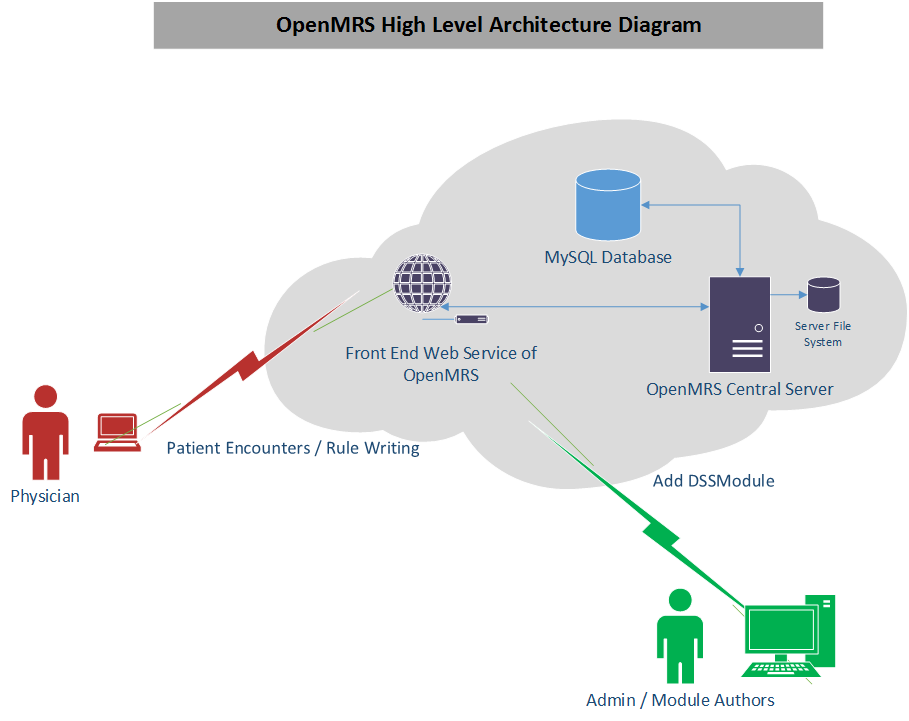
\includegraphics[width=6.5in]{OpenMRS_Architecture.png}
\end{center}
\caption{Architecture Diagram} \label{fig:ARCHITECTURE}
\end{figure}

\newpage 
\section{Decision support user guide} \label{sec:USER_GUIDE}

\subsection{Installation}
	In order to utilize the presented Decision Support System, 
and administrator must first install the module into OpenMRS. This can 
be done through the OpenMRS web interface by navigating to the "Administration" menu and following the link "Manage Modules." From there, 
click "Add or Upgrade Module"; under "Add Module", click browse. Then, 
locate and select the DSS Module file \texttt{dssmodule.omod}. Once 
this has been selected, click "Upload." OpenMRS should then install and 
start the module, and notify you of any issues with the installation 
process.

\subsection{First steps}
	Log onto OpenMRS with your corresponding username and password. Passwords are case-sensitive. Once logged in, you can search or create a patient using the tab 'Find/Create Patient'. Once you have selected the patient, their profile will appear.

\subsection{Patient profile}
	Patient profile has several tabs – Overview, Regimens, Visits, Demographics, Graphs, Form Entry, Example, Vitals, and Notes.  There is also a patient summary link and underneath are any alerts that a physician may need to be aware about the patient, as shown in Figure ~\ref{fig:PATIENT_PROFILE}.

\begin{figure}\begin{center}
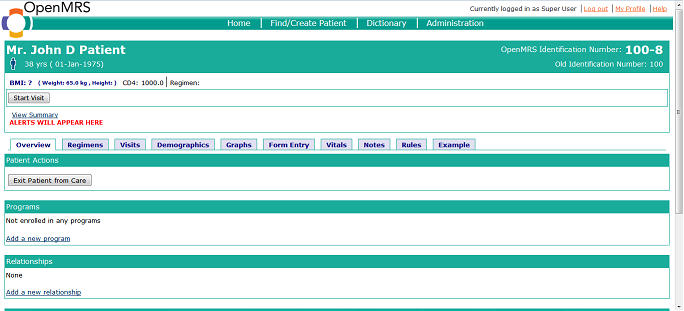
\includegraphics[width=6.5in]{user_guide/patient_profile.png}
\end{center}
\caption{Patient profile}
\label{fig:PATIENT_PROFILE}
\end{figure}

\subsubsection{Form entry}
	There are four different forms available – Vitals, Viral, Hemoglobin, and CD4 (shown in Figure ~\ref{fig:VITALS_FORM}, 
	~\ref{fig:VIRAL_FORM}, ~\ref{fig:HEMOGLOBIN_FORM}, 
	and ~\ref{fig:CD4_FORM}). Viral, Hemoglobin, and CD4 are for lab results. The encounter details must be filled along with the data entry. The Vitals form is an assessment of the current condition of the patient. Once the form is completed, press “Enter Form” and all information will be saved. 
	The forms from the last three encounters are available for viewing; for a more complete listing, check “Visits” tab.

\begin{figure}[htbp]
\begin{center}
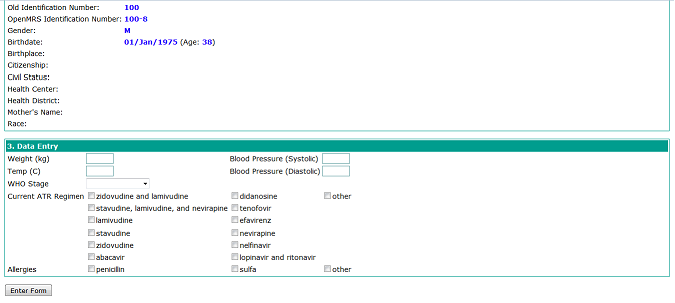
\includegraphics[width=6.5in]{user_guide/vitals_form.png}
\end{center}
\caption{Vitals form}
\label{fig:VITALS_FORM}
\end{figure}

\begin{figure}[htbp]
\begin{center}
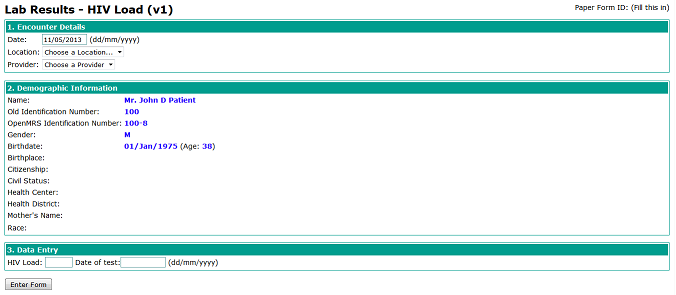
\includegraphics[width=6.5in]{user_guide/viral_form.png}
\end{center}
\caption{Viral form}
\label{fig:VIRAL_FORM}
\end{figure}

\begin{figure}[htbp]
\begin{center}
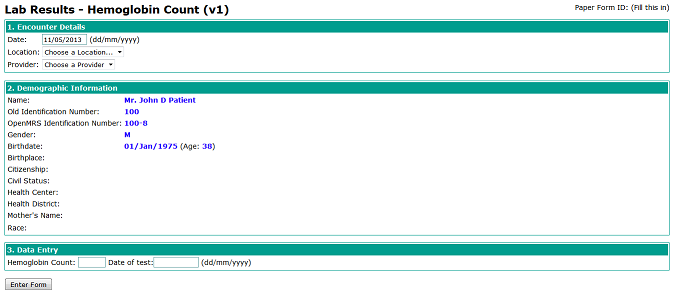
\includegraphics[width=6.5in]{user_guide/hemoglobin_form.png}
\end{center}
\caption{Hemoglobin form}
\label{fig:HEMOGLOBIN_FORM}
\end{figure}

\begin{figure}[htbp]
\begin{center}
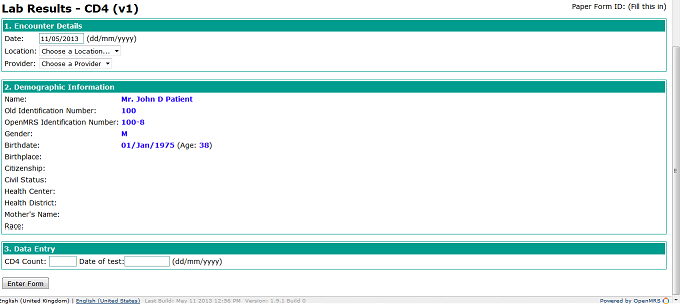
\includegraphics[width=6.5in]{user_guide/cd4_form.png}
\end{center}
\caption{CD4 form}
\label{fig:CD4_FORM}
\end{figure}

\newpage
\subsubsection{Vitals tab}
	Displays the weight, systolic blood pressure, diastolic blood pressure, and temperature of the patient based the latest encounter without having to pull out the form. This tab is 
shown in Figure ~\ref{fig:VITALS_TAB}.

\begin{figure}[htbp]
\begin{center}
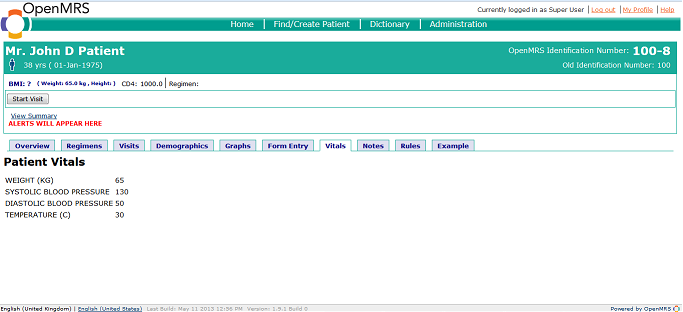
\includegraphics[width=6.5in]{user_guide/vitals_tab.png}
\end{center}
\caption{Vitals tab, displaying weight, blood pressure, and temperature 
based on latest encounter.}
\label{fig:VITALS_TAB}
\end{figure}

\subsubsection{Patient summary}
	Includes allergies, all ART regimen drugs, who stage, and TB status; it also includes the vitals of the patient from the first encounter and the last encounter; and all lab results – viral, hemoglobin, and cd4. Any alerts that a physician may need to be aware of are displayed in the bottom of the page in large bold letters, as shown in Figure ~\ref{fig:PATIENT_SUMMARY}. These information are all based on patient encounters.

\begin{figure}[htbp]
\begin{center}
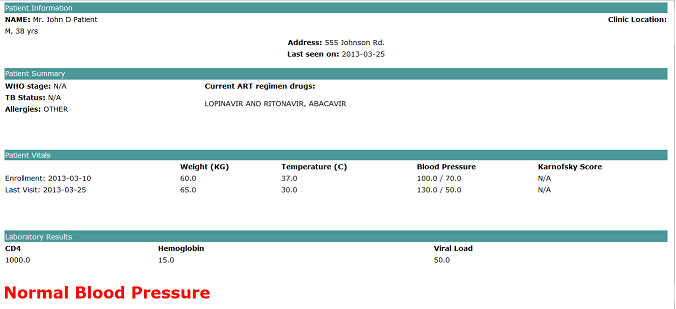
\includegraphics[width=6.5in]{user_guide/patient_summary.png}
\end{center}
\caption{Patient summary}
\label{fig:PATIENT_SUMMARY}
\end{figure}


\subsubsection{Alerts}
	Alerts are generated based on DSS rules on OpenMRS which utilizes information from patient encounters. They can be found in two locations – patient dashboard and patient summary. Figure ~\ref{fig:PATIENT_PROFILE} and ~\ref{fig:PATIENT_SUMMARY} show these rules as they appear, in bold red letters.

\subsection{Rule administration}
	Under “Administration” and under the heading “DSS Compiler” there are two links that provides you a way to create new rules onto OpenMRS, shown in Figure ~\ref{fig:ADMINISTRATION_PAGE}. Once rules are loaded onto the system, they cannot be deleted. A loading image may appear while the rules are rendering prohibiting you from using the page, it will disappear once it is done.

There are two options for managing rules: The link "Upload a DSS File" takes you to pages described in Section ~\ref{sec:UPLOAD_DSS}, and "Create DSS File" takes you to the 
page shown in Figure ~\ref{fig:CREATE_MODIFY} and described in 
Sections ~\ref{sec:LOAD_RULE}, ~\ref{sec:CREATE_RULE}, and 
~\ref{sec:SAVE_RULE}.

\begin{figure}[htbp]
\begin{center}
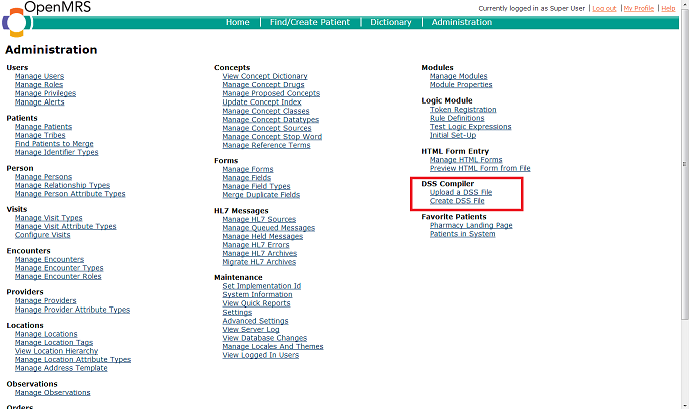
\includegraphics[width=6.5in]{user_guide/administration.png}
\end{center}
\caption{Administration page}
\label{fig:ADMINISTRATION_PAGE}
\end{figure}

\begin{figure}[htbp]
\begin{center}
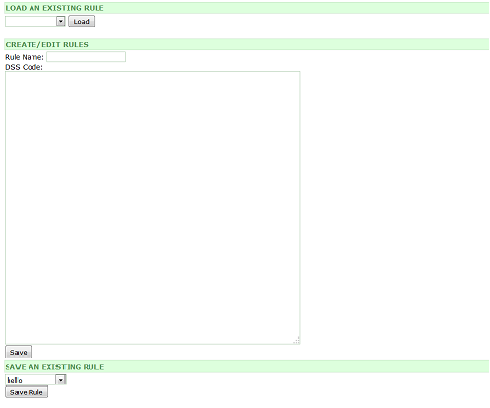
\includegraphics[width=6.5in]{user_guide/create_modify.png}
\end{center}
\caption{Create/Modify DSS Rule}
\label{fig:CREATE_MODIFY}
\end{figure}

\newpage
\subsubsection{Upload a DSS rule} \label{sec:UPLOAD_DSS}
	You can upload an existing .DSS file onto OpenMRS. Simply click Browse and locate the file you want to upload, select it, and click “upload”, as seen in Figure ~\ref{fig:UPLOAD_BROWSE}. 
	
	If there are any errors, it will be reported back and the file would not have been saved. Otherwise, the rule will be executing, as indicated in Figure ~\ref{fig:UPLOAD_SUCCESS}.

\begin{figure}[htbp]
\begin{center}
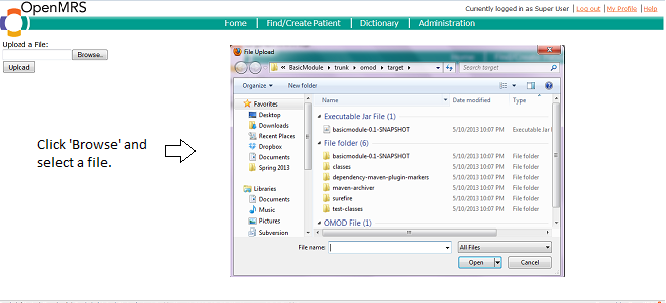
\includegraphics[width=6.5in]{user_guide/upload_browse.png}
\end{center}
\caption{DSS rule upload}
\label{fig:UPLOAD_BROWSE}
\end{figure}

\begin{figure}[htbp]
\begin{center}
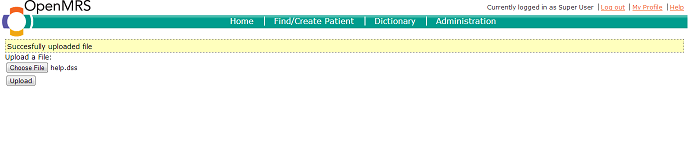
\includegraphics[width=6.5in]{user_guide/upload_success.png}
\end{center}
\caption{DSS rule upload confirmation}
\label{fig:UPLOAD_SUCCESS}
\end{figure}


\subsubsection{Load or modify an existing rule} \label{sec:LOAD_RULE}

Select an existing rule from the drop-down menu that you would like to modify then click 'Load', as seen 
in Figure ~\ref{fig:LOAD_RULE}.
It will populate the textboxes under the “Create/Edit Rule” section, as shown in Figure ~\ref{fig:LOAD_RULE_SHOWN}.

\begin{figure}[htbp]
\begin{center}
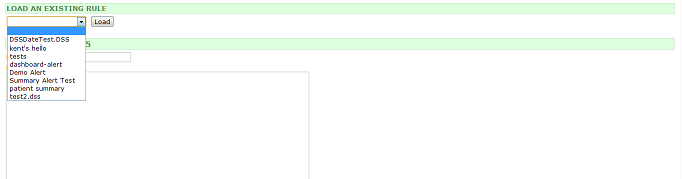
\includegraphics[width=6.5in]{user_guide/load_rule.png}
\end{center}
\caption{Loading an existing rule using the drop down menu}
\label{fig:LOAD_RULE}
\end{figure}

\begin{figure}[htbp]
\begin{center}
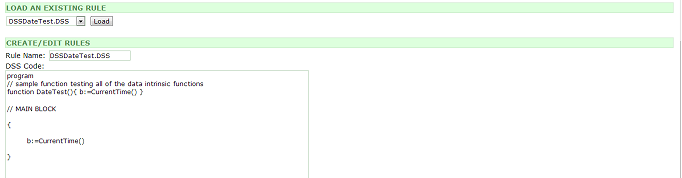
\includegraphics[width=6.5in]{user_guide/load_rule_shown.png}
\end{center}
\caption{Loaded rule displayed in text area}
\label{fig:LOAD_RULE_SHOWN}
\end{figure}

Edit the file. Once complete, click 'Save'. A confirmation message, shown in Figure ~\ref{fig:MODIFY_CONFIRMATION}, will appear to ensure that you would like to overwrite an existing rule. Click yes to save the changes.


\begin{figure}[htbp]
\begin{center}
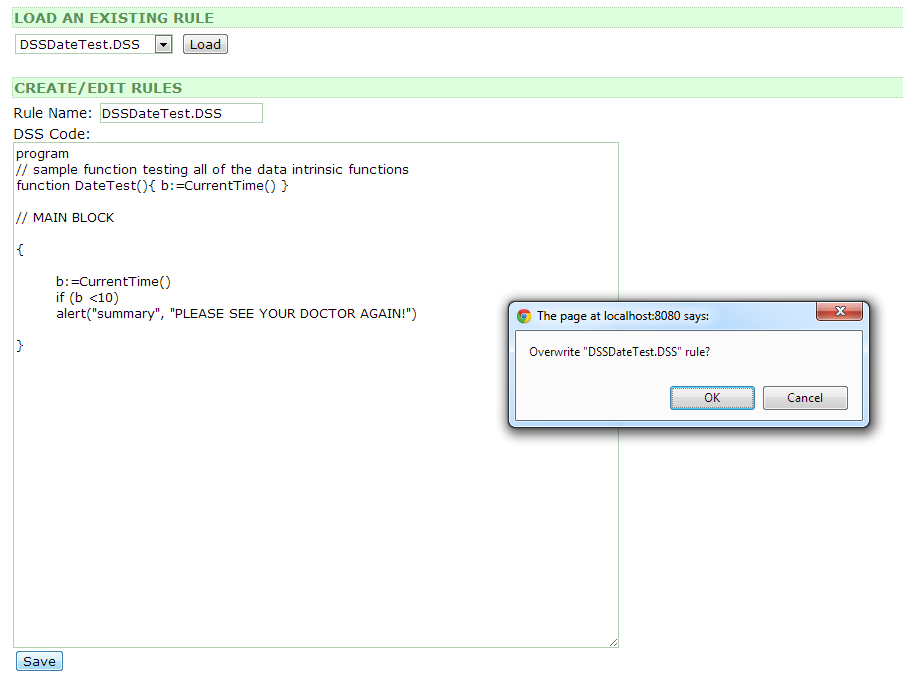
\includegraphics[width=6.5in]{user_guide/modify_confirmation.png}
\end{center}
\caption{Confirmation message, shown before over-writing an existing rule}
\label{fig:MODIFY_CONFIRMATION}
\end{figure}

A 'Successfully uploaded file' message, as shown in 
Figure ~\ref{fig:MODIFY_ERROR}, will appear if there were no errors in the program. 
If there are any errors, it will be reported back at the top of the page, as in Figure ~\ref{fig:MODIFY_SUCCESS}, and it would not have saved the changes. 
The code will still be available for you to work on it.


\begin{figure}[htbp]
\begin{center}
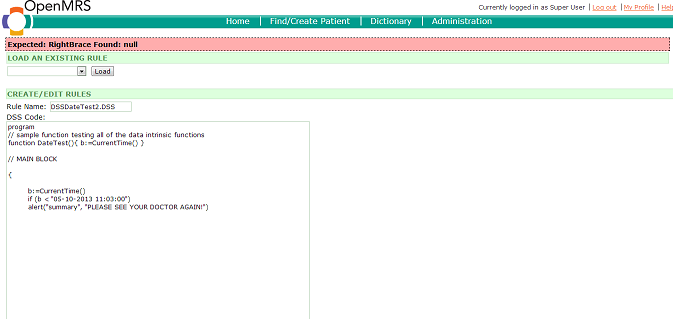
\includegraphics[width=6.5in]{user_guide/modify_error.png}
\end{center}
\caption{Error message shown when DSS code cannot be compiled}
\label{fig:MODIFY_ERROR}
\end{figure}

\begin{figure}[htbp]
\begin{center}
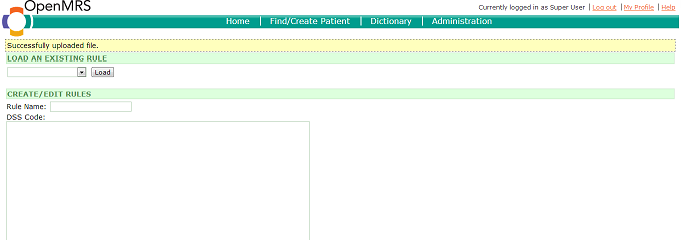
\includegraphics[width=6.5in]{user_guide/modify_success.png}
\end{center}
\caption{Confirmation message shown when DSS code has compiled successfully}
\label{fig:MODIFY_SUCCESS}
\end{figure}

\newpage
\subsubsection{Create a rule} \label{sec:CREATE_RULE}
You can create your own rule, it should not match an existing rule. Enter a rule name for the rule and enter the program under the textbox 'DSS Code' Once finished, click 'Save', as shown in Figure ~\ref{fig:NEW_RULE}.

A 'Successfully uploaded file' message will appear if there were no errors in the program and the rule name will become available in the drop down menu, as shown in Figure ~\ref{fig:NEW_RULE_SUCCESS}.
If there are any errors, it will be reported back at the top of the page and it would not have saved the changes. The code will still be available for you to work on it.

\begin{figure}[htbp]
\begin{center}
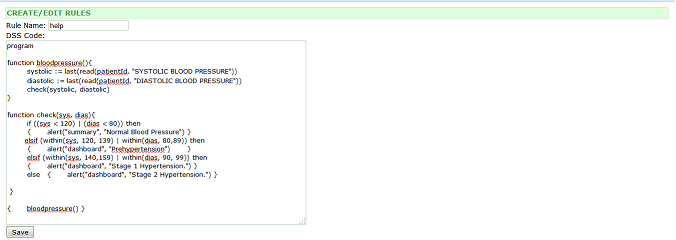
\includegraphics[width=6.5in]{user_guide/new_rule.png}
\end{center}
\caption{Creating a new rule}
\label{fig:NEW_RULE}
\end{figure}

\begin{figure}[htbp]
\begin{center}
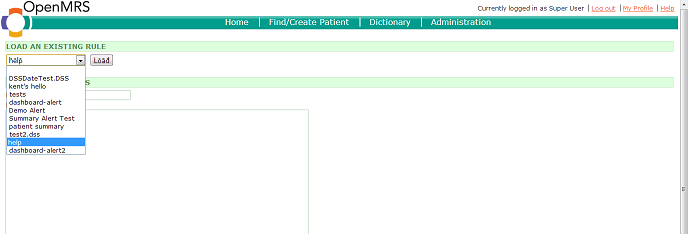
\includegraphics[width=6.5in]{user_guide/new_rule_success.png}
\end{center}
\caption{New rule after submission, shown in drop down menu}
\label{fig:NEW_RULE_SUCCESS}
\end{figure}

\newpage
\subsubsection{Save an existing rule} \label{sec:SAVE_RULE}
An existing rule can be saved on to your local file system. Choose the rule that you would like to save from the drop-down menu,  as shown in Figure ~\ref{fig:SAVE_RULE}.
Click 'Save Rule' and a download attachment window should appear, 
as shown in Figure ~\ref{fig:SAVE_RULE_DIALOG}. You can choose to either open the file or save the file. The file will be saved to your designated Downloads folder.


\begin{figure}[htbp]
\begin{center}
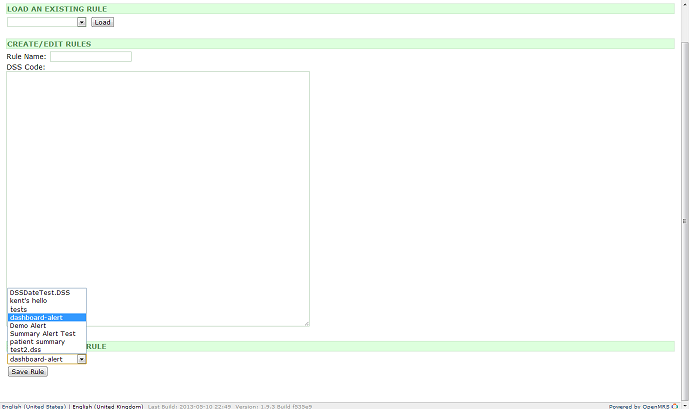
\includegraphics[width=6.5in]{user_guide/save_rule.png}
\end{center}
\caption{Choosing a rule to save locally}
\label{fig:SAVE_RULE}
\end{figure}

\begin{figure}[htbp]
\begin{center}
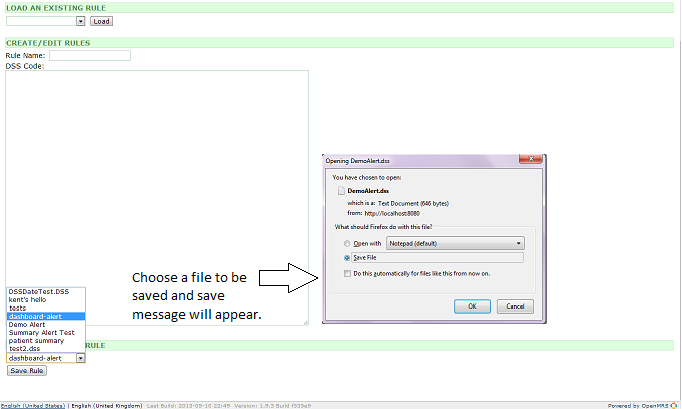
\includegraphics[width=6.5in]{user_guide/save_rule_dialog.png}
\end{center}
\caption{Browser dialog shown when attempting to save rule}
\label{fig:SAVE_RULE_DIALOG}
\end{figure}

\newpage 
\section{Use cases} \label{sec:USE_CASES}

Two main actors may interact directly with behaviors exposed in the 
DSS rule module: Administrators, who are responsible for maintaining 
the OpenMRS instance, and physicians, who utilize OpenMRS to 
support their interactions with patients. Either administrators 
or physicians may be responsible for authoring and maintaining 
rules, effectively creating a third category of actors. This 
distinction is relevant to understanding that physicians who see 
and respond to the alerts produced by rules may or may not be the 
same individuals who author those rules. Figure ~\ref{fig:USE_CASE_OVERVIEW} summarizes these interactions.

As a precondition to all use cases, an administrator is assumed to 
have installed the DSS rule module.

\begin{figure}\begin{center}
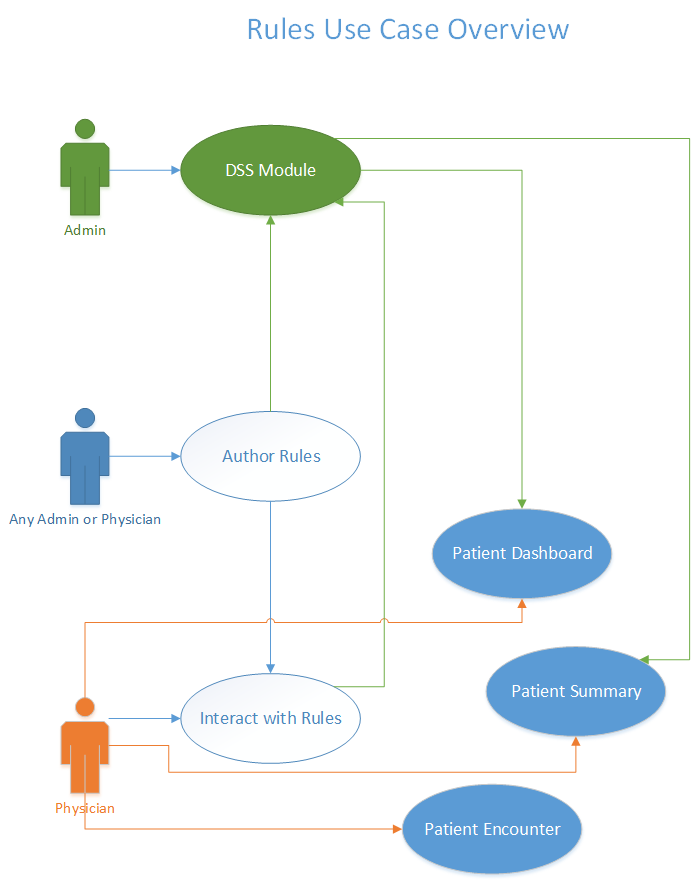
\includegraphics[height=6.5in]{use_case_overview.png}
\end{center}
\caption{Use case overview}
\label{fig:USE_CASE_OVERVIEW}
\end{figure}

\subsection{Authoring rules}

As discussed, a rule author may be either a physician or some 
form of administrator. Rule authorship and maintenance can be 
summarized by two tasks: Creating rules, described in 
Table ~\ref{tab:CREATE_RULE_USE_CASE} and 
Figure ~\ref{fig:CREATE_RULE_SEQUENCE},
and modifying existing rules, described in 
Table ~\ref{tab:MODIFY_RULE_USE_CASE} and 
Figure ~\ref{fig:MODIFY_RULE_SEQUENCE}.

\begin{table}
\begin{centering}
\begin{tabular}{ |  >{\bfseries}l | p{5in} |} \hline
Use case         &
1                \\ \hline
Use case name    &
Create Rule      \\ \hline
Summary          &
Administrator or physician can create, load, or edit rules. \\ \hline
Dependency       &
Knowledge of source code \\ \hline
Actor            &
Any administrator or physician \\ \hline
Precondition     &
Default settings \\ \hline
Description      &
Rule author navigates to Create/Modify DSS Rule page. \newline
Rule author enters a rule name and DSS Code. \newline
Rule is saved.    \newline
Rule author is able to edit or modify that rule. \\ \hline
Alternative      & 
If errors are present, rule author is notified. Rule entry form is 
not cleared, allowing error to be corrected.
\\ \hline
Postcondition    &
Rule is subsequently executed when navigating to patient 
summary or patient dashboard. \newline
Alerts produced by rule are shown where appropriate. \\ \hline
\end{tabular}
\end{centering}
\caption{Rule creation use case} \label{tab:CREATE_RULE_USE_CASE}
\end{table}

\begin{figure}\begin{center}
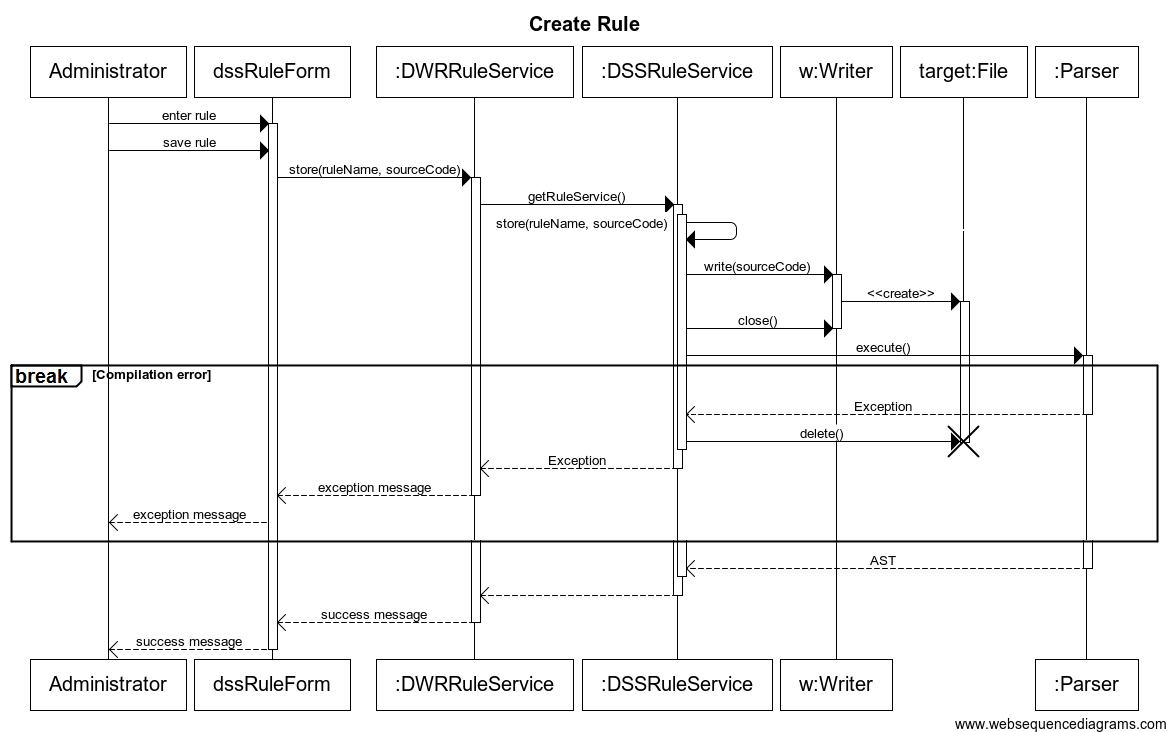
\includegraphics[width=6.5in]{sequence/create_rule.png}
\end{center}
\caption{Rule creation sequence diagram} 
\label{fig:CREATE_RULE_SEQUENCE}
\end{figure}


\begin{table}
\begin{centering}
\begin{tabular}{ |  >{\bfseries}l | p{5in} |} \hline
Use case &
2 \\ \hline
Use case name &
Modify Rule \\ \hline
Summary &
Administrator or physician can make changes to a rule. \\ \hline
Dependency &
Knowledge of source code \\ \hline
Actor &
Any adminstrator or physician \\ \hline
Precondition &
An existing rule previously saved \\ \hline
Description &
Rule author navigates to Create/Modify DSS Rule page. \newline
Rule author selects name of rule from drop down and hits "Load." \newline
Rule author makes necessary changes to a rule within the source code. \newline
Rule author hits save and confirms the modification when prompted.
\\ \hline
Alternative      & 
If errors are present, rule author is notified. Rule entry form is 
not cleared, allowing error to be corrected. \\ \hline
Postcondition &
Subsequent rule executions and alerts will exhibit the behavior specified in 
the modified rule.
 \\ \hline
\end{tabular}
\end{centering}
\caption{Rule modification use case} \label{tab:MODIFY_RULE_USE_CASE}
\end{table}

\begin{figure}\begin{center}
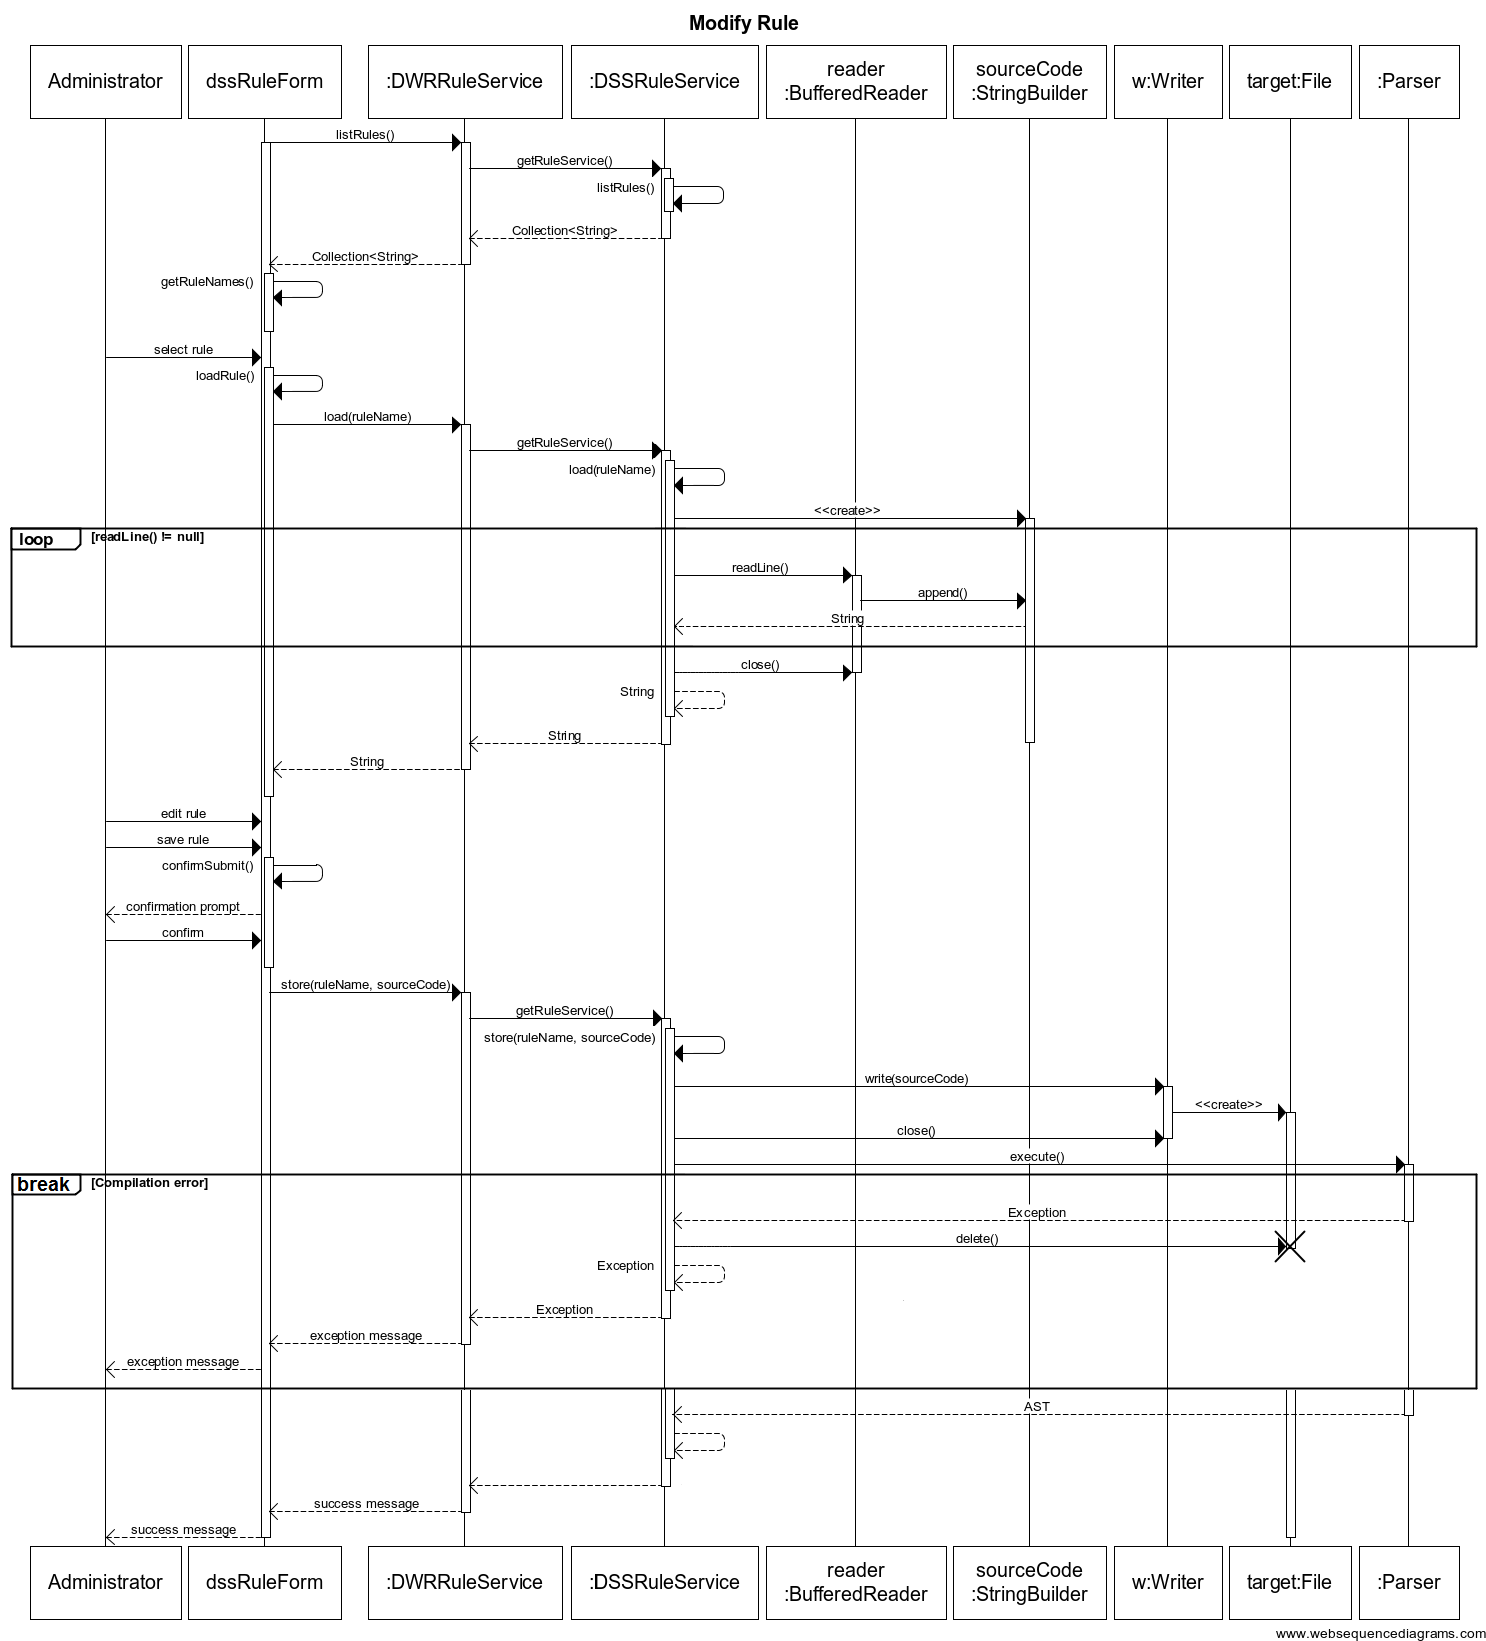
\includegraphics[width=6.5in]{sequence/modify_rule.png}
\end{center}
\caption{Rule modification sequence diagram} 
\label{fig:MODIFY_RULE_SEQUENCE}
\end{figure}

\subsection{Alerts}

The useful product of DSS rules is the alerts which they may generate, 
which can inform the actions a physician may subsequently take. Alerts 
are shown in two contexts: On the patient dashboard, as described in 
Table ~\ref{tab:PATIENT_DASHBOARD_USE_CASE} and 
Figure ~\ref{fig:PATIENT_DASHBOARD_SEQUENCE},
and within the patient summary, as described in 
Table ~\ref{tab:PATIENT_SUMMARY_USE_CASE} and 
Figure ~\ref{fig:PATIENT_SUMMARY_SEQUENCE}.

\begin{table}
\begin{centering}
\begin{tabular}{ |  >{\bfseries}l | p{5in} |} \hline
Use case &
3 \\ \hline
Use case name &
Patient Dashboard \\ \hline
Summary & 
Encounter information and relevant alerts are made available 
for a specific patient. \\ \hline
Dependency &
Log in to OpenMRS. \\ \hline
Actor &
Physician \\ \hline
Precondition &
An existing patient has been created. \\ \hline
Description &
Physician searches for a patient and navigates to patient dashboard. \newline
Medical information recorded on the patient is accessible through tabs for greater detail. \newline
Rules for patient are executed and any alerts for the "dashboard" target 
are displayed near the top of the page. \newline
A link to the Patient Summary page is provided near the top of the page.
\\ \hline
Alternative &
\\ \hline
Postcondition &
Physician may navigate among patient dashboard tabs containing 
patient information. \newline
Physician may navigate to patient summary. \newline
Physician has been notified with relevant alerts produced by defined 
DSS rules.
\\ \hline
\end{tabular}
\end{centering}
\caption{Patient dashboard use case} \label{tab:PATIENT_DASHBOARD_USE_CASE}
\end{table}

\begin{figure}\begin{center}
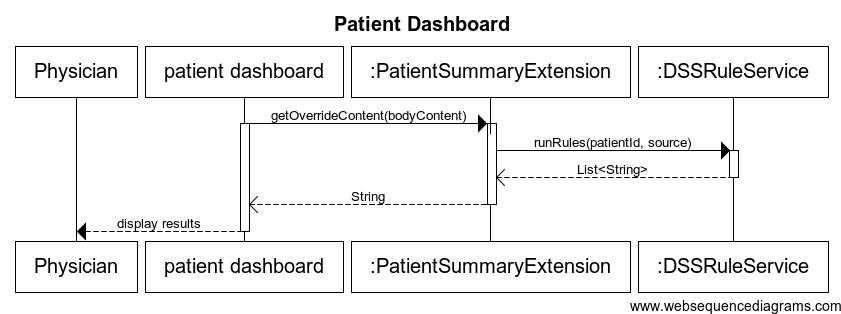
\includegraphics[width=6.5in]{sequence/patient_dashboard.png}
\end{center}
\caption{Patient dashboard sequence diagram} 
\label{fig:PATIENT_DASHBOARD_SEQUENCE}
\end{figure}

\begin{table}
\begin{centering}
\begin{tabular}{ |  >{\bfseries}l | p{5in} |} \hline
Use case &
4 \\ \hline
Use case name &
Patient Summary \\ \hline
Summary & 
Major information of a patient is displayed. \\ \hline
Dependency &
Patient Dashboard \\ \hline
Actor &
Physician \\ \hline
Precondition &
Relevant encounter data for the patient. \\ \hline
Description &
Physician clicks "Patient Summary" link from Patient Dashboard. \newline
Patient summary displays the main medical information including the WHO stage, TB Status, Allergies, and current drugs. \newline
Rules are executed, and any alerts for the "summary" target are 
displayed at the bottom of the page.
\\ \hline
Alternative &
\\ \hline
Postcondition &
Physician has summary information about the patient. \newline
Physician has been notified with relevant alerts produced by defined 
DSS rules.
\\ \hline
\end{tabular}
\end{centering}
\caption{Patient summary use case} \label{tab:PATIENT_SUMMARY_USE_CASE}
\end{table}

\begin{sidewaysfigure}\begin{center}
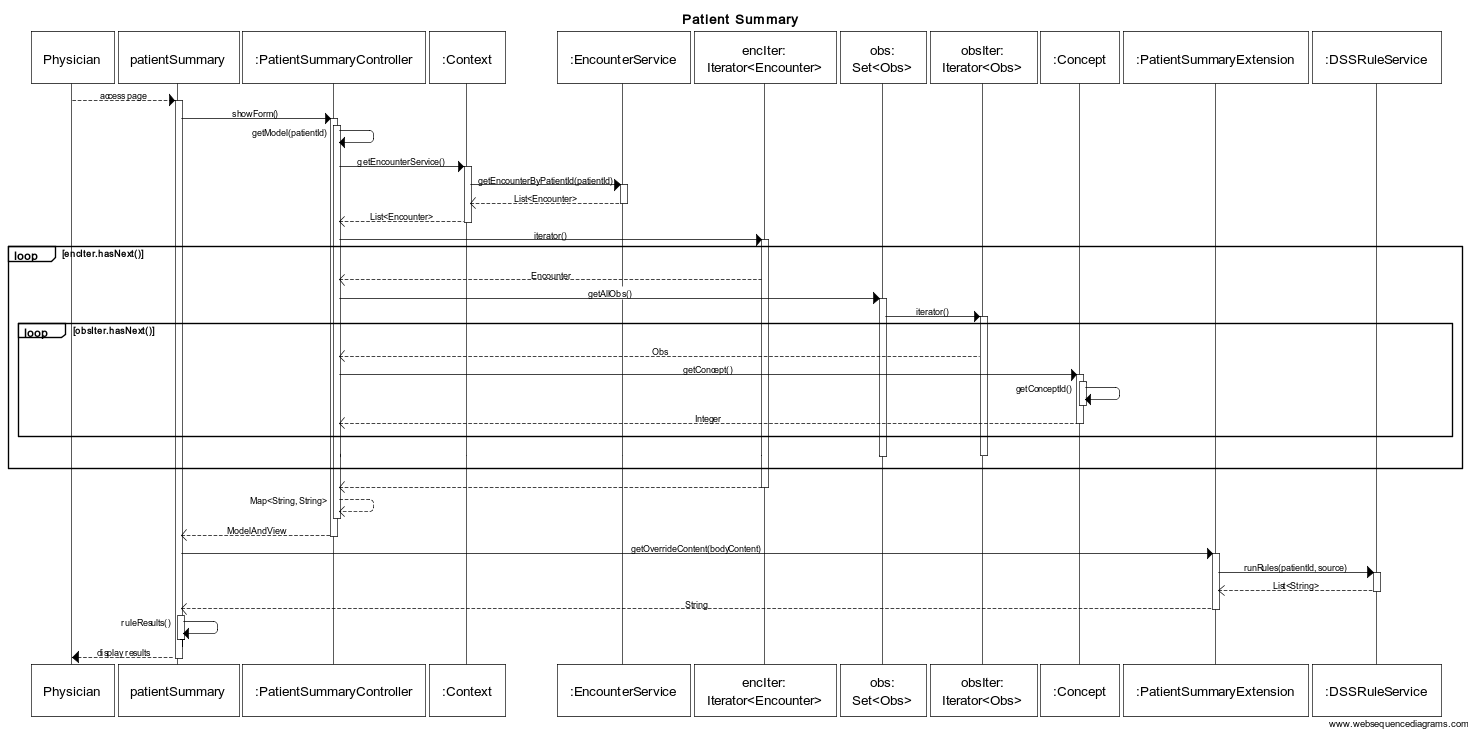
\includegraphics[width=8in]{sequence/patient_summary.png}
\end{center}
\caption{Patient summary sequence diagram} 
\label{fig:PATIENT_SUMMARY_SEQUENCE}
\end{sidewaysfigure}


\newpage 
\section{Design overview} \label{sec:DESIGN_OVERVIEW}

	The DSS1 rule subsystem is incorporated into OpenMRS in a simple Client-Server fashion. The target implementation will feature client-side web pages which interact with the DSS1 rule subsystem on the server by way of DSSRuleService. Figure ~\ref{fig:TIERS} illustrates this interaction.

\tikzstyle{layer}=[rectangle, 
                   rounded corners,
                   draw=black, 
                   align=center,
                   anchor=north]
\tikzstyle{communicates}=[draw, ->, >=triangle 60]
\tikzstyle{boundary}=[draw, -, dashed]
\begin{figure}\begin{center}
\begin{tikzpicture}
\node (Client) [layer] { 
  \textbf{Client Pages}      \\
  Patient Summary \\
  Patient Dashboard \\
  DSS Rule Administration
};
\node (Boundary) [below=of Client, minimum width=3in] {};
\node [above=of Boundary.east] {\emph{Client}};
\node [below=of Boundary.east] {\emph{Server}};
\node (Service) [layer, below=of Boundary] { 
  \textbf{DSS Rule Service}  \\
  Run rules  \\
  List rules \\
  Add rules  \\
  Edit rules
};
\node (Interpreter) [layer, below=of Service] { 
  \textbf{DSS1 Interpreter}  \\
  Intrinsics  \\
  Evaluations \\
  Flow control
};
\path [communicates] (Client) -- (Service) {};
%\path [communicates] (Service.115    ) -- (Client.240     ) {};
\path [communicates] (Service) -- (Interpreter) {};
%\path [communicates] (Interpreter.120) -- (Service.245    ) {};
\path [boundary] (Boundary.180) -- (Boundary.0    ) {};
%\path [boundary]     (Boundary.west  ) -- (Boundary.east  ) {};
\end{tikzpicture}
\caption{Usage relationship of major tiers.}\label{fig:TIERS}
\end{center}\end{figure}

The DSS Rule Service, in turn, utilizing the DSS1 Interpreter subsystem to run rules and report results.

While the DSS Rule Service runs on the server, its interface is exposed to client-side JavaScript code via DWR (Direct Web Remoting).

\subsection{Client pages} \label{sec:CLIENT_PAGES}

Multiple client web pages interact with the DSS Rule Service.

\subsubsection{Patient summary} \label{sec:PATIENT_SUMMARY}

The Patient Summary ({\texttt{patientsummary.jsp}) is  stand-alone page, reachable from a link on the Patient Dashboard. It is used primarily to contain major information about a patient (gender, age, WHO stage, etc.) The Patient Summary invokes the rule service via DWR to retrieve all alerts for the named target  \texttt{summary} and displays them below other patient information. 

\subsubsection{Patient Dashboard} \label{sec:PATIENT_DASHBOARD}

The Patient Dashboard is the primary landing point for viewing patient information, and contains multiple tabs for this purpose. This extension inserts a link to the Patient Summary on the Patient Dashboard, and accompanies this with relevant alerts by invoking the rule service for the \texttt{dashboard} target.

See \texttt{org.openmrs.module.basicmodule.extension.html.PatientSummaryExtension}

\subsubsection {DSS Rule Administration} 
\label{sec:DSS_RULE_ADMINISTRATION}

Create DSS Rule (\texttt{dssRules.form}) provides a form where DSS source code can be entered and submitted to the rule service with a specific rule name. Consolidates the ability to create new rules, load existing rules, and edit rules in one form. Made accessible through an extension to the Administration menu.

\subsection{Rule service} \label{sec:RULE_SERVICE}

The DSSRuleService follows the facade design pattern to expose important functionality to clients. The high-level tasks that are relevant to client code are defined using a few simple methods which hide the details of compiling, interpreting, and managing the storage of rules. Specific functionality is detailed in table ~\ref{tab:RULE_SERVICE}.

\begin{table}
\begin{center}
\begin{tabular}{ l | p{1.25in} | p{2.25in} }
Method & Description & Details \\ \hline

\texttt{getRuleService()}
&
Static method to retrieve an instance of the rule service.
&
Constructs a new DSSRuleService object, if necessary. During 
constructor call any existing rules are loaded from the file 
system, using the DSSXMLConvertor to convert from XML to DOM to AST.
\\ \hline

\texttt{store(rule, code)}
&
Stores a rule (either as a new rule, or replacing an existing rule) with the given source code.
&
Invokes the Parser to convert source code to AST; 
Invokes the DSSXMLConvertor to convert AST to DOM and save; 
Saves the original source to file system for subsequent retrieval; 
Stores the AST in memory for subsequent running.
\\ \hline

\texttt{load(rule)}
&
Load the source code for an existing rule.
&
Reads stored source code from the file system.
\\ \hline

\texttt{listRules()}
&
List all existing rules.
&
Returns a list of all stored rule names.
\\ \hline

\texttt{runRules(patientId, target)}
&
Get all alerts for the given target (“summary” or “dashboard”) as appropriate to the given patient.
&
For each rule:
Construct interpreter; 
Install intrinsics, including “alert” function which stores to a map;
Pre-define “patientId” for DSS1 program;
Run the interpreter on the rule.
Thereafter, pull all alerts appropriate to the target from the map.
\\ \hline

\end{tabular}
\end{center}
\caption{Methods exposed by the DSS Rule Service}
\label{tab:RULE_SERVICE}
\end{table}

\subsubsection{Rule storage} \label{sec:RULE_STORAGE}

On upload, rules are compiled to an Abstract Syntax Tree (AST) form 
using the provided Parser class. Once compiled successfully, the rule is stored to the OpenMRS application data directory. 

Each rule is  stored in two formats: Plain text source code, and an XML (Extensible Markup Language) representation of the compiled AST. The 
source code is subsequently used only to support user interactions (for instance, if an administrator wants to load or modify source for an existing rule). The XML form is used when the DSS Rule Service is first initialized to load any existing rules from the file system. After initialization, rules are stored in memory as AST objects.

The utility class DSSXMLConvertor is used for conversion between AST and XML. Internally, the class maintains a Document Object Model (DOM) representation of the AST. This can be either as loaded from an XML file, or as formed by traversing an AST. Likewise, DSSXMLConvertor provides methods for both producing AST objects or writing XML files.

\subsection{Interpreter} \label{sec:INTERPRETER}

The Interpreter is implemented with four distinct sub systems, as depicted in Figure ~\ref{fig:INTERPRETER}.
At the top level, \emph{flow control} is provided by the InterpreterVisitor, which is responsible for traversing the Abstract Syntax Tree. An \emph{execution context} is maintained to describe the running state of the system, including defined variables and functions. While tree traversal coordinates complex expressions, the actual \emph{evaluation} of expressions is itself implemented in a distinct set of classes representing the types available under DSS1. Finally, a library of \emph{intrinsic functions} is provided in order to mediate interactions with OpenMRS from running DSS1, as well as to provide certain convenience functions to DSS1 rule programmers.

\tikzstyle{system}=[rectangle,
                   thick, 
                   draw=black, 
                   align=center,
                   anchor=north]
\tikzstyle{connects}=[draw, ->, >=triangle 60]
\tikzstyle{observes}=[draw, ->, dashed, >=triangle 60]
\begin{figure}
\begin{center}
\begin{tikzpicture}[node distance=1.5in]
\node (FlowControl) [system] 
      {\textbf{Flow control}};
\node (Middle) [below=of FlowControl] {};
\node (ExecutionContext) [system, left=of Middle] 
      {\textbf{Execution context}};
\node (Evaluation) [system, below=of Middle] 
      {\textbf{Evaluation}};
\node (IntrinsicFunction) [system, right=of Middle] 
      {\textbf{Intrinsic functions}};
\draw [connects] (FlowControl) -- (ExecutionContext) {}
      node [midway,above,sloped] {Sets, gets state} ;
\draw [connects] (ExecutionContext) -- (Evaluation) {}
      node [midway,below,sloped] {Contains values} ;
\draw [connects] (ExecutionContext) -- (IntrinsicFunction) {}
      node [midway,below left,sloped] {Contains functions} ;
\draw [connects] (FlowControl) -- (IntrinsicFunction) {}
      node [midway,above,sloped] {Invokes} ;
\draw [connects] (IntrinsicFunction) -- (Evaluation) {}
      node [midway,below,sloped] {Yields values} ;
\draw [connects] (FlowControl) -- (Evaluation) {}
      node [midway,above,sloped] {Assembles complex expressions} ;
\end{tikzpicture}
\end{center}
\caption{High-level overview of the DSS1 Interpreter.}
\label{fig:INTERPRETER}
\end{figure}

\subsubsection{Flow control} \label{sec:FLOW_CONTROL}

	Flow control in the interpreter is implemented using the Visitor design pattern, traversing the Abstract Syntax Tree (AST) produced by the existing Compiler using an implementation of the provided ASTVisitor interface, performing computation as appropriate at every given node in the tree.

	The Visitor design pattern leverages double dispatch to decouple a data structure from the operations which can be performed while traversing this data structure. The Visitor calls an \texttt{accept} method on a node within the data structure, which is itself overloaded to call a more specific method on the Visitor itself; \texttt{visitBlockTree}, for example. This permits the external object – the Visitor – to implement behavior using the data structure's type hierarchy, without adding that specific behavior to those types directly.

	In the case of the Interpreter, the data structure is the AST, which describes a DSS1 program as a tree of elements – block (BlockTree), if statements (IfTree), et cetera. The Visitor is the IntepreterVisitor, which manages and performs the computation described by this program. This is done with the support of other underlying subsystems to describe variable state and perform type-specific evaluations, as described in the Architecture section.

	The class InterpreterVisitor acts as the center of a subsystem  responsible for high-level interpretation of the program, including flow control, and coordinating complex expressions.

\subsubsection{Execution context} \label{sec:EXECUTION_CONTEXT}

The ExecutionContext class provides a means to store and retrieve return values, variable states, and named functions. It also handles rules of scope to hide variables during function calls, and exposes the Evaluator. Note that this may be populated with functions or even variables before being given to the InterpreterVisitor, allowing the definition of intrinsics and constants (such as \texttt{patientId}).

Functions stored in the ExecutionContext are of type DSSFunction, which is an interface used to describe any function called from DSS1 (either intrinsic or user-defined). This permits function calling to be implemented identically for both categories of function. Additionally includes a method for testing if a given argument should be passed as a raw identifier instead of evaluated directly (as used by some intrinsics.).

Similarly, variables and return values are stored as DSSValue 
objects, with their specific implementation defined within the 
evaluation subsystem.

\subsubsection{Evaluation of expressions} \label{sec:EVALUATION}

The abstract class DSSValue describes a set of operations which can be performed on values in DSS1 as methods, as well as the common state (the potential to store time stamps). Its concrete sub-classes, such as DSSValueInt, DSSValueFloat, et cetera, provide specific implementations of these operations in order to define the behavior of their DSS1 type. Additionally, concrete subclasses of DSSValue typically are defined with some field to maintain their specific value (for instance, DSSValueBool has an underlying Java \texttt{boolean} field to describe its value.)

The Evaluator interface and DSSEvaluator implementation exposes methods to perform operations upon DSS1 values, to interpret literals, allocate DSS objects, and perform conversions between DSS1 values and similar Java objects. The Evaluator serves as intermediary between flow control and the specific semantics implemented in DSSValue types; this facilitates separation of concerns, allowing the gradual introduction of new DSS1 data types while avoiding changes to  flow control.

Finally, a DSSValueFactory class is provided to aid in the instantiation of DSSValue objects. This class utilizes the Factory design pattern to allow new values to be created (for instance, as the return values of intrinsic functions) without requiring users of those values to have specific knowledge of the DSSValue subclasses actually used.

\subsubsection{Intrinsic functions} \label{sec:INTRINSIC_FUNCTIONS}

DSSLibrary defines an interface for delivering or generating intrinsic functions in related groupings. Each function is returned in a map where the name should be used to call the function from a DSS program, and the function object is used as a Java object that extends the DSSFunction. These functions may then be easily installed into the ExecutionContext used by the Intepreter before running rules. A list of libraries used in this implementation is presented in Table ~\ref{tab:LIBRARIES}.

This approach supports extensibility of the DSS rule module. 
Rather than being built into the DSS1 Interpreter at the language 
level, intrinsic functions can be contained and communicated 
as DSSLibrary objects. Adding intrinsics is then as simple as 
defining a new DSSLibrary and installing it to the execution context before running rules.

The ReadLibrary serves as an interesting example case, at it illustrates interaction with the OpenMRS platform without requiring specific knowledge of this platform from other elements of the interpreter. The read functions retrieve a list of observations associated with a patient. The first parameter of the functions, patientId, is a numeric identifier unique to each patient. The second parameter, conceptName, is the word or phrase used by the OpenMRS dictionary to refer to a concept. 

The three functions are nearly identical, save for one difference: while read() returns a list containing all observations that match the function parameters, readInitialEncounter() and readLatestEncounter() filter out results based on the timestamp of the observations. Calling readInitialEncounter() retrieves only the observations from the patient's earliest encounter on record, while readLatestEncounter() retrieves only the observations from the patient's most recent encounter on record. 

When the functions are called, they retrieve a list of all encounters associated with patientId from the OpenMRS database. The functions iterate through these lists, and in the case of readInitialEncounter() and readLatestEncounter(), the timestamp for each encounter is checked. If the timestamp does not meet the criteria, the encounter is discarded. Once an encounter has been verified as valid the function shall retrieve all observations associated with the encounter. Each observation shall have its concept name checked against conceptName, and matches are added to the list of observations that each function shall return. 

Observations consist of three pieces of data: the value of the observation, the data type of the observation value, and the time of the observation. Internally, observations are represented as DSSValue objects, which store the value of the observation and the time of the observation. The data type of the observation value is stored as part of the DSSValue class type itself. Both the time and data type of the observation can be retrieved using the time() and type check intrinsics, respectively. 

Note that the \texttt{alert} intrinsic is treated as a special case. Rather than being contained within a library class, it is installed directly by the DSS Rule Service into the Interpreter before running rules. This facilitates retrieval of results issued via \texttt{alert} calls.

\begin{table}
\begin{center}
\begin{tabular} { l | l }
\textbf{Library}  & \textbf{Functions implemented}\\ \hline
IsLibrary         & \texttt{isString(var)}        \\
                  & \texttt{isFloat(var)}         \\
                  & \texttt{isInt(var)}           \\
                  & \texttt{isBoolean(var)}       \\
                  & \texttt{isList(var)}          \\
                  & \texttt{isObject(var)}        \\
                  & \texttt{isDate(var)}          \\ \hline
LengthAndWithinLibrary
                  & \texttt{length(var)}          \\
                  & \texttt{within(v,a,b)}        \\ \hline
ListLibrary       & \texttt{merge(a,b)}           \\
                  & \texttt{sortTime(list)}       \\
                  & \texttt{sortData(list)}       \\
                  & \texttt{first(list)}          \\
                  & \texttt{last(list)}           \\ \hline
ReadLibrary       & \texttt{read(patientId,
                                 concept)}        \\
                  & \texttt{readInitialEncounter(patientId,
                                 concept)}        \\
                  & \texttt{readLatestEncounter(patientId,
                                 concept)}        \\ \hline
DateLibrary       & \texttt{currenttime()}        \\
                  & \texttt{recentTimeItem(list)} \\
                  & \texttt{oldestTimeItem(list)} \\
                  & \texttt{before(a,b)}          \\
                  & \texttt{time(var)}            \\
                  & \texttt{addDays(v,days)}      \\
                  & \texttt{addMonths(v,months)}  \\ \hline
\end{tabular}
\end{center}
\caption{Libraries of intrinsics}
\label{tab:LIBRARIES}
\end{table}

% \section{External documentation}

\newpage 
\section{Package structure}

Figure ~\ref{fig:PACKAGE_DIAGRAM} illustrates the usage relationships 
between packages. For brevity, only the last relevant tokens of a 
package name are used; for instance, 
\texttt{org.openmrs.module.dssmodule} has been labeled simply 
\texttt{dssmodule}.

\subsection{OpenMRS integration packages}

Multiple components support interaction with the DSS module from 
OpenMRS. These are described in Table 
~\ref{tab:INTEGRATION_PACKAGES}.

\begin{table}
\begin{center}
\begin{tabular}{ >{\tt}l | p{2.5in} }
org.openmrs.module.dssmodule &
Contains classes which define core functionality exposed to front-end 
classes or to OpenMRS directly, such as the DSSRuleService, as well 
as classes which directly support these. \\ \hline
org.openmrs.module.dssmodule.extension.html &
Describes module-introduced behavior at specific extension points 
within OpenMRS.
 \\ \hline
org.openmrs.module.dssmodule.web.controller &
Provides classes to handle web requests which support maintenance 
and execution of DSS rules. \\ \hline
\end{tabular}
\end{center}
\caption{Description of packages which support interaction with OpenMRS front-end} 
\label{tab:INTEGRATION_PACKAGES}
\end{table}

\subsection{Interpreter packages}

As described in Section ~\ref{sec:INTERPRETER}, the Interpreter is 
composed of four major sub-systems. These are defined in corresponding 
packages, as documented in Table ~\ref{tab:INTERPRETER_PACKAGES}.

\begin{table}
\begin{center}
\begin{tabular}{ >{\tt}l | p{2.5in} }
org.openmrs.module.dssmodule.flowcontrol &
Classes which handle and implement flow control for the 
DSS1 language. \\ \hline
org.openmrs.module.dssmodule.intrinsics &
Implementations of DSS1 intrinsic functions, and the libraries 
used to organize them. \\ \hline
org.openmrs.module.dssmodule.state &
Describes the execution classes and closely related classes. \\ \hline
org.openmrs.module.dssmodule.value &
Defines the specific value types available under DSS1 and 
implements their behavior. \\ \hline
\end{tabular}
\end{center}
\caption{Description of interpreter packages} \label{tab:INTERPRETER_PACKAGES}
\end{table}


\subsection{Provided packages}

At the start of this project, an existing compiler for the DSS1 language 
was provided, and has been used without significant modification. The 
packages which comprise this component are identified in Table 
~\ref{tab:PROVIDED_PACKAGES}.

\begin{table}
\begin{center}
\begin{tabular}{ >{\tt}l | p{3in} }
org.openmrs.module.dssmodule.lexer &
Provides classes which support the conversion of raw DSS1 source code 
to meaningful lexical units (tokens). \\ \hline
org.openmrs.module.dssmodule.ast &
Provides classes to describe the syntactic structure of a compiled 
DSS1 program. \\ \hline
org.openmrs.module.dssmodule.parser &
Supports parsing of DSS1 source code (using the \texttt{lexer} package) into a compiled tree structure (using the \texttt{ast} package). \\ \hline
org.openmrs.module.dssmodule.visitor &
Describes an interface for traversing a compiled AST, following the 
visitor design pattern. \\ \hline
\end{tabular}
\end{center}
\caption{Description of provided packages} \label{tab:PROVIDED_PACKAGES}
\end{table}

\tikzstyle{tab}=[rectangle, draw, anchor=south west]
\tikzstyle{package}=[rectangle, 
                   draw=black, 
                   anchor=north, align=justify]
\tikzstyle{utilizes}=[draw, ->, dashed, >=triangle 60]
\begin{figure}
\begin{center}
\begin{tikzpicture}[node distance=0.33in]


\node (ExtensionHtml) [package]  { 
AdminDSS \\
PatientSummaryExtension \\
VitalsPatientDashboardTab
} ;
\node [tab] at (ExtensionHtml.north west)
{ extension.html } ;

\node (WebController) [package, right=of ExtensionHtml]  { 
DSSRuleController \\
DSSUploadController \\
DWRRuleService \\
DWRVitalsService \\
FileDownload \\
PatientSummaryController
} ;
\node [tab] at (WebController.north west)
{ web.controller } ;

\node (Module) [package, below=of ExtensionHtml]  { 
DSSInterpreter \\
DSSModuleActivator \\
DSSRuleService \\
DSSXMLConvertor 
} ;
\node [tab] at (Module.north west)
{ dssmodule } ;





\node (Intrinsics) [package, below=of WebController]  { 
DSSLibrary \\
DateLibrary \\
IsLibrary \\
LengthAndWithinLibrary \\
ListLibrary \\
ReadLibrary \\
DSSAddDays \\
DSSAddMonths \\
...
} ;
\node [tab] at (Intrinsics.north west)
{ intrinsics } ;



\node (State) [package, below=of Intrinsics.south east]  { 
DSSEvaluator \\
DSSExecutionContext \\
DSSFunction \\
Evaluator \\
ExecutionContext \\
NamingContext
} ;
\node [tab] at (State.north west)
{ state } ;

\node (FlowControl) [package, left=of State.south west]  { 
AST \\
ActualArgsTree \\
AssignTree \\
BlockTree \\
CallTree \\
ElsifTree \\
...
} ;
\node [tab] at (FlowControl.north west)
{ flowcontrol } ;

\node (Value) [package, right=of Intrinsics]  { 
DSSValue \\
DSSValueBool \\
DSSValueDate \\
DSSValueFloat \\
DSSValueInt \\ 
... \\
DSSValueFactory
} ;
\node [tab] at (Value.north west)
{ value } ;


\node (Parser) [package, below=of Module.south west]  { 
Parser
} ;
\node [tab] at (Parser.north west)
{ parser } ;

\node (Lexer) [package, below=of Parser]  { 
Lexer \\
SourceReader \\
Symbol \\
Token \\
Tokens \\
TokenType
} ;
\node [tab] at (Lexer.north west)
{ lexer } ;

\node (AST) [package, below=of Lexer.south east]  { 
AST \\
ActualArgsTree \\
AssignTree \\
BlockTree \\
CallTree \\
ElsifTree \\
...
} ;
\node [tab] at (AST.north west)
{ ast } ;

\node (Visitor) [package, below=of AST]  { 
ASTVisitor \\
PrintVisitor
} ;
\node [tab] at (Visitor.north west)
{ visitor } ;

\path [utilizes] (ExtensionHtml) -- (WebController) {};
\path [utilizes] (WebController) -- (Module) {};
\path [utilizes] (Module.south) |- (FlowControl.north west) {};
\path [utilizes] (Module) -- (Intrinsics) {};
\path [utilizes] (FlowControl) -- (State) {};
\path [utilizes] (State) -- (Value) {};
\path [utilizes] (Intrinsics) -- (Value) {};
\path [utilizes] (FlowControl) -- (AST) {};
\path [utilizes] (Parser) -- (Lexer) {};
\path [utilizes] (Parser.east) -| (AST.80) {};
\path [utilizes] (Module.south) -- (Parser.north east) {};
\path [utilizes] (FlowControl) |- (Visitor) {};
\path [utilizes] (Module.south east) |- (State.north west) {};

\end{tikzpicture}
\end{center}
\caption{Package diagram}
\label{fig:PACKAGE_DIAGRAM}
\end{figure}


\newpage 
\section{Class diagrams} \label{sec:CLASS_DIAGRAMS}

\subsection{Classes describing flow control}

Figure ~\ref{fig:INTERPRETER_VISITOR_DIAGRAM} shows the relationship 
of classes directly involved in or utilized during the handling of flow 
control when interpreting a DSS program.

The InterpreterVisitor is used to initiate program interpretation. It 
delegates the interpretation of specific node types to corresponding 
ASTInterpreter types. It also maintains an instance of a DSSExecutionContext 
to support interactions with the running state of the program.

\subsection{Classes describing execution context}

Figure ~\ref{fig:EXECUTION_CONTEXT_DIAGRAM} describes the 
composition of the execution context. The active state of the program, 
including currently-defined functions and variable assignments, is maintained in appropriate data structures.

Each ExecutionContext additionally maintains a reference to an Evaluator 
object, which exposes necessary methods for the interpreter to interact 
with values in DSS.

\subsection{Classes describing values}

Figure ~\ref{fig:VALUE_DIAGRAM} shows the classes used to describe values in 
a running DSS program. The abstract class DSSValue describes the operations 
available under DSS1 as methods; its concrete subclasses provide 
implementations for these operations. Note that each DSSValue object also 
maintains a field for the time stamp of a value, which is populated when 
observations are read from OpenMRS services. For other values this is null.

Not shown is DSSValueFactory, which exposes methods to create DSSValue 
objects to wrap their corresponding underlying Java types.

\subsection{Classes describing intrinsics}

Figure ~\ref{fig:INTRINSIC_DIAGRAM} describes the relationship of classes 
which describe specific intrinsic functions to the classes used to 
categorize them.

Calls made by a running DSS program are resolved by a named DSSFunction 
object, as stored in the execution context. The DSSLibrary interface 
provides a useful way to group related functions along with their names 
to facilitate their installation into the execution context. 

Also shown is the DeclaredFunction class. A DeclaredFunction is created 
for user-defined functions in a DSS program, and contains references to 
appropriate nodes within the AST to support actual interpretation of the 
function call, as well as the visitor used to perform interpretation, and 
the execution context, which is used to handle the change in variable 
scope associated with the function call.

\tikzstyle{class}=[rectangle, 
                   draw=black, 
                   rectangle split, 
                   rectangle split parts=3,
                   align=center,
                   anchor=north]
\tikzstyle{implements}=[draw, ->, >=open triangle 90]
\tikzstyle{aggregates}=[draw, <-, >=open diamond]
\tikzstyle{contains}=[draw, <-, >=diamond]

\begin{figure}
\begin{center}
\begin{tikzpicture}[node distance=0.25in]
\node (ASTVisitor) [class] { 
  \emph{ASTVisitor}
  \nodepart{second}  
  \nodepart[align=justify]{third}
  + visitBlockTree(t : AST) \\
  + visitIdTree(t : AST)    \\
  + visitCallTree(t : AST)  \\
  ...
};
\node (InterpreterVisitor) [class, below=of ASTVisitor] { 
  \textbf{InterpreterVisitor}
  \nodepart{second}  
  \nodepart[align=justify]{third}
};

\node (DSSExecutionContext) [class, right=of InterpreterVisitor] { 
  \textbf{DSSExecutionContext}
  \nodepart{second}  
  \nodepart[align=justify]{third}
  + setConstant(name : String,  value : DSSValue) \\
  + setIntrinsic(name : String,  func : DSSFunction)
};
\node (ExecutionContext) [class, above=of DSSExecutionContext] { 
  \textbf{ExecutionContext}
  \nodepart[align=justify]{second}  
  - evaluator : Evaluator
  \nodepart[align=justify]{third}
  + beginScope() \\
  + endScope() \\
  + getEvaluator() : Evaluator \\
  + getFunction(name : String) : DSSFunction \\
  + getReturnValue() : DSSValue \\
  + setReturnValue(v : DSSValue) \\
  + setFunction(name : String, f : DSSFunction)
};
\node (ASTInterpreter) [class, below=of InterpreterVisitor.south east] { 
  \emph{ASTInterpreter}
  \nodepart{second}  
  \nodepart[align=justify]{third}
  + interpret(ast : AST, 
              c : ExecutionContext, 
              v : ASTVisitor) \\ \hspace{10pt} : Object
};

\node (IdInterpreter) [class, below=of ASTInterpreter] { 
  \textbf{IdInterpreter}
  \nodepart{second}  
  \nodepart[align=justify]{third}
};
\node (BlockInterpreter) [class, left=of IdInterpreter] { 
  \textbf{BlockInterpreter}
  \nodepart{second}  
  \nodepart[align=justify]{third}
};
\node (CallInterpreter) [class, right=of IdInterpreter] { 
  \textbf{CallInterpreter}
  \nodepart{second}  
  \nodepart[align=justify]{third}
};
\node () [right=of CallInterpreter] {...};


\node (NamingContext) [class, above=of ExecutionContext] { 
  \emph{NamingContext}
  \nodepart[align=justify]{third}
  +set (name : String, value : DSSValue) \\
  +get (name : String) : DSSValue
};

\path [implements] (ExecutionContext) -- (NamingContext) {};
\path [implements] (InterpreterVisitor) -- (ASTVisitor) {};
\path [implements] (BlockInterpreter) -- (ASTInterpreter) {};
\path [implements] (IdInterpreter) -- (ASTInterpreter) {};
\path [implements] (CallInterpreter) -- (ASTInterpreter) {};
\path [implements] (DSSExecutionContext) -- (ExecutionContext) {};
\path [contains] (InterpreterVisitor) -- (DSSExecutionContext) {};
\path [contains] (InterpreterVisitor) -- (ASTInterpreter) {};
\draw (InterpreterVisitor) -- (ASTInterpreter) 
      node [midway, right] {\small{1..*}};
\draw (InterpreterVisitor) -- (DSSExecutionContext) 
      node [midway, above] {\small{1..1}};
\end{tikzpicture}
\end{center}
\caption{Interpreter visitor}
\label{fig:INTERPRETER_VISITOR_DIAGRAM}
\end{figure}

\begin{figure}
\begin{tikzpicture}[node distance=0.33in]
\node (ExecutionContext) [class] { 
  \textbf{ExecutionContext}
  \nodepart[align=justify]{second}  
  - functions : Map\textless String, DSSFunction\textgreater \\
  - variables : Map\textless String, DSSValue\textgreater \\
  - scope : Stack\textless Map\textless String, DSSValue\textgreater \textgreater \\
  - returnValue : DSSValue \\
  - evaluator : Evaluator
  \nodepart[align=justify]{third}
  + beginScope() \\
  + endScope() \\
  + getEvaluator() : Evaluator \\
  + getFunction(name : String) : DSSFunction \\
  + getReturnValue() : DSSValue \\
  + setReturnValue(v : DSSValue) \\
  + setFunction(name : String, f : DSSFunction)
};
\node (DSSValue) [class, right=of ExecutionContext] { 
  \emph{DSSValue}
  \nodepart[align=justify]{second}  
  - timestamp : Date
  \nodepart[align=justify]{third}
  + add (v : DSSValue) : DSSValue \\
  + sub (v : DSSValue) : DSSValue \\
  + div (v : DSSValue) : DSSValue \\
  ... \\
  + getTimeStamp() : Date
};
\node (NamingContext) [class, above=of ExecutionContext] { 
  \emph{NamingContext}
  \nodepart[align=justify]{third}
  +set (name : String, value : DSSValue) \\
  +get (name : String) : DSSValue
};
\node (DSSFunction) [class, right=of NamingContext] { 
  \emph{DSSFunction}
  \nodepart{second}  
  \nodepart[align=justify]{third}
  + call(args : DSSValue[]) : DSSValue \\
  + passAsIdentifier(argIndex : int) \\ \hspace{10pt} : boolean
};

\node (Evaluator) [class, below=of ExecutionContext] { 
  \emph{Evaluator}
  \nodepart{second}  
  \nodepart[align=justify]{third}
  + castTo(javaClass : Class, v : DSSValue) : Object \\
  + evaluate(leftOper : DSSValue, \\ 
    \hspace{10pt} operator : String, \\
    \hspace{10pt} rightOper : DSSValue) : DSSValue\\
  + evaluateLiteral(lit : Symbol) : DSSValue \\
  + newAllocation(fields : String[]) : DSSValue \\
  + toDSSValue(javaObject : Object) : DSSValue
};
\node (DSSEvaluator) [class, right=of Evaluator] { 
  \textbf{DSSEvaluator}
  \nodepart{second}  
  \nodepart[align=justify]{third}
};


\path [aggregates] (ExecutionContext) -- (DSSValue) {};
\path [aggregates] (ExecutionContext) -- (DSSFunction) {};
\path [contains] (ExecutionContext) -- (Evaluator) {};
\path [implements] (ExecutionContext) -- (NamingContext) {};
\path [implements] (DSSEvaluator) -- (Evaluator) {};
\draw (ExecutionContext) -- (DSSValue) 
      node [midway, above] {\small{1..*}};
\draw (ExecutionContext) -- (DSSFunction) 
      node [midway, below] {\small{1..*}};

\end{tikzpicture}
\caption{Execution context class diagram}
\label{fig:EXECUTION_CONTEXT_DIAGRAM}
\end{figure}

\begin{figure}
\begin{center}
\begin{tikzpicture}[node distance=0.25in]
\node (DSSValue) [class] { 
  \emph{DSSValue}
  \nodepart[align=justify]{second}  
  - timestamp : Date
  \nodepart[align=justify]{third}
  + add (v : DSSValue) : DSSValue \\
  + sub (v : DSSValue) : DSSValue \\
  + div (v : DSSValue) : DSSValue \\
  + mul (v : DSSValue) : DSSValue \\
  + power (v : DSSValue) : DSSValue \\
  + concat (v : DSSValue) : DSSValue \\
  + and (v : DSSValue) : DSSValue \\
  + or (v : DSSValue) : DSSValue \\
  + equal (v : DSSValue) : boolean \\
  + notequal (v : DSSValue) : boolean \\
  + lessthan (v : DSSValue) : boolean \\
  + greaterthan (v : DSSValue) : boolean \\
  + lessthanequal (v : DSSValue) : boolean \\
  + greaterthanequal (v : DSSValue) : boolean \\
  + getTimeStamp() : Date \\
  + setTimeStamp(date : Date)
};

\node (DSSValueNumeric) [class, right=of DSSValue.north east] {
  \emph{DSSValueNumeric}
  \nodepart[align=justify]{second}  
  \nodepart[align=justify]{third}
};
\node (DSSValueFloat) [class, above=of DSSValueNumeric] {
  \textbf{DSSValueFloat}
  \nodepart[align=justify]{second}  
  - value : double
  \nodepart[align=justify]{third}
};
\node (DSSValueInt) [class, below=of DSSValueNumeric] {
  \textbf{DSSValueInt}
  \nodepart[align=justify]{second}  
  - value : long
  \nodepart[align=justify]{third}
};
\node (DSSValueBool) [class, below=of DSSValueInt] {
  \textbf{DSSValueBool}
  \nodepart[align=justify]{second}  
  - value : boolean
  \nodepart[align=justify]{third}
};
\node (DSSValueString) [class, below=of DSSValueBool] {
  \textbf{DSSValueString}
  \nodepart[align=justify]{second}  
  - value : String
  \nodepart[align=justify]{third}
};
\node (DSSValueList) [class, below=of DSSValueString] {
  \textbf{DSSValueList}
  \nodepart[align=justify]{second}  
  - value : List
  \nodepart[align=justify]{third}
};
\node (DSSValueObject) [class, below=of DSSValue] {
  \textbf{DSSValueObject}
  \nodepart[align=justify]{second}  
  - fields : Map\textless String, DSSValue\textgreater 
  \nodepart[align=justify]{third}
};
\node (DSSValueNull) [class, right=of DSSValueObject] {
  \textbf{DSSValueNull}
  \nodepart[align=justify]{second}  
  \nodepart[align=justify]{third}
};

\node (NamingContext) [class, below=of DSSValueObject] { 
  \emph{NamingContext}
  \nodepart[align=justify]{third}
  +set (name : String, value : DSSValue) \\
  +get (name : String) : DSSValue
};

\path [implements] (DSSValueInt) -- (DSSValueNumeric) {};
\path [implements] (DSSValueFloat) -- (DSSValueNumeric) {};
\path [implements] (DSSValueNumeric) -- (DSSValue) {};
\path [implements] (DSSValueBool) -- (DSSValue) {};
\path [implements] (DSSValueString) -- (DSSValue) {};
\path [implements] (DSSValueList) -- (DSSValue) {};
\path [implements] (DSSValueNull) -- (DSSValue) {};
\path [implements] (DSSValueObject) -- (DSSValue) {};
\path [implements] (DSSValueObject) -- (NamingContext) {};
\end{tikzpicture}
\end{center}
\caption{Value class diagram}
\label{fig:VALUE_DIAGRAM}
\end{figure}

\begin{figure}
\begin{center}
\begin{tikzpicture}[node distance=0.25in]
\node (DSSLibrary) [class] { 
  \emph{DSSLibrary}
  \nodepart[align=justify]{second}  
  \nodepart[align=justify]{third}
  +getFunctions(context : ExecutionContext) : 
      Map \textless String, DSSFunction\textgreater
};

\node (ReadLibrary) [class, below=of DSSLibrary] { 
  \textbf{ReadLibrary}
  \nodepart[align=justify]{second}  
  \nodepart[align=justify]{third}
};

\node (DateLibrary) [class, left=of ReadLibrary] { 
  \textbf{DateLibrary}
  \nodepart[align=justify]{second}  
  \nodepart[align=justify]{third}
};

\node (ListLibrary) [class, right=of ReadLibrary] { 
  \textbf{ListLibrary}
  \nodepart[align=justify]{second}  
  \nodepart[align=justify]{third}
};

\node (DSSRead) [class, below=of ReadLibrary] { 
  \textbf{DSSRead}
  \nodepart[align=justify]{second}  
  \nodepart[align=justify]{third}
};

\node (DSSReadInitialEncounter) [class, left=of DSSRead] { 
  \textbf{DSSReadInitialEncounter}
  \nodepart[align=justify]{second}  
  \nodepart[align=justify]{third}
};

\node (DSSReadLatestEncounter) [class, right=of DSSRead] { 
  \textbf{DSSReadLatestEncounter}
  \nodepart[align=justify]{second}  
  \nodepart[align=justify]{third}
};

\node (DSSFunction) [class, below=of DSSRead] { 
  \emph{DSSFunction}
  \nodepart{second}  
  \nodepart[align=justify]{third}
  + call(args : DSSValue[]) : DSSValue \\
  + passAsIdentifier(argIndex : int)  : boolean
};

\node (DeclaredFunction) [class, below=of DSSFunction] { 
  \textbf{DeclaredFunction}
  \nodepart[align=justify]{second}  
  formals : FormalsTree \\
  block : BlockTree \\
  context : ExecutionContext \\
  visitor : ASTVisitor
  \nodepart[align=justify]{third}
};

\node () [left=of DateLibrary] {...};
\node () [right=of ListLibrary] {...};
\node () [left=of DSSReadInitialEncounter] {...};
\node () [right=of DSSReadLatestEncounter] {...};


\path [contains] (ReadLibrary) -- (DSSRead) {};
\path [contains] (ReadLibrary) -- (DSSReadInitialEncounter) {};
\path [contains] (ReadLibrary) -- (DSSReadLatestEncounter) {};
\path [implements] (ReadLibrary) -- (DSSLibrary) {};
\path [implements] (DateLibrary) -- (DSSLibrary) {};
\path [implements] (ListLibrary) -- (DSSLibrary) {};
\path [implements] (DSSRead) -- (DSSFunction) {};
\path [implements] (DSSReadInitialEncounter) -- (DSSFunction) {};
\path [implements] (DSSReadLatestEncounter) -- (DSSFunction) {};
\path [implements] (DeclaredFunction) -- (DSSFunction) {};


\end{tikzpicture}
\end{center}
\caption{Intrinsic class diagram}
\label{fig:INTRINSIC_DIAGRAM}
\end{figure}

\newpage \appendix 
\section{DSS1 language specification} \label{sec:LANGUAGE}

\subsection{Grammar}

\begin{verbatim}
 PROGRAM -> ‘program’ D* BLOCK ==> program
 BLOCK -> ‘{‘ S* ‘}’  ==> block
 D -> 'function' NAME FUNHEAD BLOCK      	==> functionDecl
 FUNHEAD  -> '(' (NAME list ',')? ')'  	==> formals
 S -> ‘if’ EE ‘then’ BLOCK ('else' BLOCK)? ==> if 
   -> ‘if’ EE ‘then’ BLOCK Elif ==> if 
   -> ‘while’ EE BLOCK               		==> while
   -> 'for' NAME in NLIST BLOCK     		==> FOR
   -> ‘return’ EE                    		==> return
   -> BLOCK
   -> IdMod’:=‘ EE                    		==> assign
   -> NAME '(' (EE list ',')? ')' 		==> call
 
  Elif -> ‘elsif’ EE 'then' BLOCK Elif			==> elsif
-> ‘elsif’ EE 'then' BLOCK ('else' BLOCK)?	==> elsif
  
  EE 	-> E
  	-> EE '||' E
  
  E 	-> SE
  	-> SE ‘==‘ SE   	==> =
  	-> SE ‘!=‘ SE   	==> !=
  	-> SE ‘<‘  SE   	==> <
  	-> SE ‘<=‘ SE   	==> <=
 
  SE 	->  T
  	->  SE ‘+’ T  	==> +
  	->  SE ‘-’ T  	==> -
  	->  SE ‘|’ T  	==> or
 
  T  	-> TT
  	-> T ‘*‘ F  	==> *
  	-> T ‘/’ F  	==> /
  	-> T ‘&’ F  	==> and
 
  TT 	-> F
  	-> TT ** F    	==> **
 
  F  	-> ‘(‘ EE ‘)’
  	-> IdMod 
  	-> <literal>
  	-> NAME '(' (EE list ',')? ')' 		==> call
  	-> Object '(' (NAME list ',')? ')'    ==> ObjectDecl
  	-> new NAME          				==> Object
  	-> LIST
  IdMod -> NAME
        -> NAME '.' NAME    			==> fieldRef
  
  NLIST	-> NAME
       	-> LIST
  
  LIST	-> '{' (E list ',')? '}'   		==> list
 
  NAME	-> <id>
\end{verbatim}

\subsection {Intrinsic functions}

	Several built-in functions may be utilized when writing a DSS program, as listed in Table ~\ref{tab:INTRINSIC_FUNCTION_LIST}. Function names are case sensitive.

\begin{table}\begin{centering}
\begin{tabular}{ | >{\tt}l | p{3.66in} | }
\hline
isString(v) & 
Check if \texttt{v} is of type string; returns a boolean. \\ \hline
isInt(v) & 
Check if \texttt{v} is of type integer; returns a boolean. \\ \hline
isFloat(v) & 
Check if \texttt{v} is of type float; returns a boolean. \\ \hline
isBoolean(v) & 
Check if \texttt{v} is of type boolean; returns a boolean. \\ \hline
isDate(v) & 
Check if \texttt{v} is of type date; returns a boolean. \\ \hline
isObject(v) & 
Check if \texttt{v} is of type object; returns a boolean. \\ \hline
isList(v) & 
Check if \texttt{v} is of type list; returns a boolean. \\ \hline
\hline
currenttime() &
Returns current system time, as a date. \\ \hline
recentTimeItem(list) &
Returns the item in the list with the most recent time. \\ \hline
oldestTimeItem(list) &
Returns the item with the oldest time. \\ \hline
before(t1, t2) &
Returns true if \texttt{t1} is before \texttt{t2} \\ \hline
time(v) &
Returns the time associated with \texttt{v} \\ \hline
addDays(time, n) &
Returns a new date, \texttt{n} days after \texttt{time}.
\\ \hline
addMonths(time, n) &
Returns a new date, \texttt{n} months after \texttt{time}.
\\ \hline \hline
merge(list1, list2) &
Returns a new list containing all items from \texttt{list1} and 
\texttt{list2}, sorted chronologically.  \\ \hline
sortTime(list) &
Returns a new list sorted based on time of items 
\\ \hline
sortData(list) &
Returns a new list sorted based on values of items  \\ \hline
last(list) &
Returns the last item in the list \\ \hline
first(list) &
Returns the first in the list \\ \hline
\hline
read(p, c) &
Returns a list of observations of concept \texttt{c} for the specified patient \texttt{p} from database. \newline
\texttt{c} should match the name given in the Concept Dictionary. 
\\ \hline
readInitialEncounter(p,c) &
Returns a list of observations for patient \texttt{p} and concept 
\texttt{c} from database, only from the initial encounter.
\\ \hline
readLatestEncounter(p,c) &
Returns a list of observations for patient \texttt{p} and concept 
\texttt{c} from database, only from the latest encounter.
\\ \hline \hline
alert(target, message) &
Send an alert to a target;
\texttt{target} can either be \texttt{summary} (for Patient Summary) or \texttt{dashboard} (for Patient Dashboard)
\\ \hline
within(v, a, b) &
Returns true if \texttt{v} is between \texttt{a} and \texttt{b}, inclusive.
\\ \hline
length(v) &
Returns the length of a list or a string. \\ \hline
\end{tabular}


\end{centering}
\caption{DSS1 intrinsic functions} \label{tab:INTRINSIC_FUNCTION_LIST}
\end{table}

\newpage
\section{Test cases} \label{sec:TEST_CASES}

\subsection{Language testing} \label{sec:TEST_CASES_LANGUAGE}

\subsubsection{Source code for language test}
\lstinputlisting{languageTest.dss}

\subsubsection{Results for language test}
\begin{footnotesize}
\lstinputlisting{languageResults.txt}
\end{footnotesize}

\subsection{Intrinsic function testing} \label{sec:TEST_CASES_INTRINSICS}

\subsubsection{Source code for comprehensive intrinsics test}
\lstinputlisting{basicTest.dss}

\subsubsection{Results for comprehensive intrinsics test}
\begin{footnotesize}
\lstinputlisting{basicResults.txt}
\end{footnotesize}

\subsubsection{Source code for example test (blood pressure)}
\lstinputlisting{bpTest.dss}

\subsubsection{Results for example test (blood pressure)}
\begin{footnotesize}
\lstinputlisting{bpResults.txt}
\end{footnotesize}

\subsubsection{Source code for example test (temperature)}
\lstinputlisting{tempTest.dss}

\subsubsection{Results for example test (temperature)}
\begin{footnotesize}
\lstinputlisting{tempResults.txt}
\end{footnotesize}

\newpage
\section{API Documentation} \label{sec:API_DOCS}

% Import javadoc; temporarily suppress including subsections in TOC
\setcounter{tocdepth}{1}
\section*{Class Hierarchy}{
\thispagestyle{empty}
\markboth{Class Hierarchy}{Class Hierarchy}
\addcontentsline{toc}{section}{Class Hierarchy}
\subsection*{Classes}
{\raggedright
\hspace{0.0cm} $\bullet$ java.lang.Object {\tiny \refdefined{java.lang.Object}} \\
\hspace{1.0cm} $\bullet$ AdministrationSectionExt {\tiny } \\
\hspace{2.0cm} $\bullet$ org.openmrs.module.dssmodule.extension.html.AdminDSS {\tiny \refdefined{org.openmrs.module.dssmodule.extension.html.AdminDSS}} \\
\hspace{1.0cm} $\bullet$ Extension {\tiny } \\
\hspace{2.0cm} $\bullet$ org.openmrs.module.dssmodule.extension.html.PatientSummaryExtension {\tiny \refdefined{org.openmrs.module.dssmodule.extension.html.PatientSummaryExtension}} \\
\hspace{1.0cm} $\bullet$ PatientDashboardTabExt {\tiny } \\
\hspace{2.0cm} $\bullet$ org.openmrs.module.dssmodule.extension.html.RulesPatientDashboardTab {\tiny \refdefined{org.openmrs.module.dssmodule.extension.html.RulesPatientDashboardTab}} \\
\hspace{2.0cm} $\bullet$ org.openmrs.module.dssmodule.extension.html.VitalsPatientDashboardTab {\tiny \refdefined{org.openmrs.module.dssmodule.extension.html.VitalsPatientDashboardTab}} \\
\hspace{1.0cm} $\bullet$ java.lang.Enum {\tiny \refdefined{java.lang.Enum}} \\
\hspace{2.0cm} $\bullet$ org.openmrs.module.dssmodule.lexer.Tokens {\tiny \refdefined{org.openmrs.module.dssmodule.lexer.Tokens}} \\
\hspace{1.0cm} $\bullet$ org.openmrs.module.dssmodule.DSSInterpreter {\tiny \refdefined{org.openmrs.module.dssmodule.DSSInterpreter}} \\
\hspace{1.0cm} $\bullet$ org.openmrs.module.dssmodule.DSSModuleActivator {\tiny \refdefined{org.openmrs.module.dssmodule.DSSModuleActivator}} \\
\hspace{1.0cm} $\bullet$ org.openmrs.module.dssmodule.DSSRuleService {\tiny \refdefined{org.openmrs.module.dssmodule.DSSRuleService}} \\
\hspace{1.0cm} $\bullet$ org.openmrs.module.dssmodule.DSSXMLConvertor {\tiny \refdefined{org.openmrs.module.dssmodule.DSSXMLConvertor}} \\
\hspace{1.0cm} $\bullet$ org.openmrs.module.dssmodule.ast.AST {\tiny \refdefined{org.openmrs.module.dssmodule.ast.AST}} \\
\hspace{2.0cm} $\bullet$ org.openmrs.module.dssmodule.ast.ActualArgsTree {\tiny \refdefined{org.openmrs.module.dssmodule.ast.ActualArgsTree}} \\
\hspace{2.0cm} $\bullet$ org.openmrs.module.dssmodule.ast.AssignTree {\tiny \refdefined{org.openmrs.module.dssmodule.ast.AssignTree}} \\
\hspace{2.0cm} $\bullet$ org.openmrs.module.dssmodule.ast.BlockTree {\tiny \refdefined{org.openmrs.module.dssmodule.ast.BlockTree}} \\
\hspace{2.0cm} $\bullet$ org.openmrs.module.dssmodule.ast.CallTree {\tiny \refdefined{org.openmrs.module.dssmodule.ast.CallTree}} \\
\hspace{2.0cm} $\bullet$ org.openmrs.module.dssmodule.ast.ElsifTree {\tiny \refdefined{org.openmrs.module.dssmodule.ast.ElsifTree}} \\
\hspace{2.0cm} $\bullet$ org.openmrs.module.dssmodule.ast.FieldRefTree {\tiny \refdefined{org.openmrs.module.dssmodule.ast.FieldRefTree}} \\
\hspace{2.0cm} $\bullet$ org.openmrs.module.dssmodule.ast.ForTree {\tiny \refdefined{org.openmrs.module.dssmodule.ast.ForTree}} \\
\hspace{2.0cm} $\bullet$ org.openmrs.module.dssmodule.ast.FormalsTree {\tiny \refdefined{org.openmrs.module.dssmodule.ast.FormalsTree}} \\
\hspace{2.0cm} $\bullet$ org.openmrs.module.dssmodule.ast.FunctionDeclTree {\tiny \refdefined{org.openmrs.module.dssmodule.ast.FunctionDeclTree}} \\
\hspace{2.0cm} $\bullet$ org.openmrs.module.dssmodule.ast.IdTree {\tiny \refdefined{org.openmrs.module.dssmodule.ast.IdTree}} \\
\hspace{2.0cm} $\bullet$ org.openmrs.module.dssmodule.ast.IfTree {\tiny \refdefined{org.openmrs.module.dssmodule.ast.IfTree}} \\
\hspace{2.0cm} $\bullet$ org.openmrs.module.dssmodule.ast.ListTree {\tiny \refdefined{org.openmrs.module.dssmodule.ast.ListTree}} \\
\hspace{2.0cm} $\bullet$ org.openmrs.module.dssmodule.ast.LiteralTree {\tiny \refdefined{org.openmrs.module.dssmodule.ast.LiteralTree}} \\
\hspace{2.0cm} $\bullet$ org.openmrs.module.dssmodule.ast.ObjectDeclTree {\tiny \refdefined{org.openmrs.module.dssmodule.ast.ObjectDeclTree}} \\
\hspace{2.0cm} $\bullet$ org.openmrs.module.dssmodule.ast.ObjectTree {\tiny \refdefined{org.openmrs.module.dssmodule.ast.ObjectTree}} \\
\hspace{2.0cm} $\bullet$ org.openmrs.module.dssmodule.ast.OpTree {\tiny \refdefined{org.openmrs.module.dssmodule.ast.OpTree}} \\
\hspace{2.0cm} $\bullet$ org.openmrs.module.dssmodule.ast.ProgramTree {\tiny \refdefined{org.openmrs.module.dssmodule.ast.ProgramTree}} \\
\hspace{2.0cm} $\bullet$ org.openmrs.module.dssmodule.ast.ReturnTree {\tiny \refdefined{org.openmrs.module.dssmodule.ast.ReturnTree}} \\
\hspace{2.0cm} $\bullet$ org.openmrs.module.dssmodule.ast.WhileTree {\tiny \refdefined{org.openmrs.module.dssmodule.ast.WhileTree}} \\
\hspace{1.0cm} $\bullet$ org.openmrs.module.dssmodule.flowcontrol.AssignInterpreter {\tiny \refdefined{org.openmrs.module.dssmodule.flowcontrol.AssignInterpreter}} \\
\hspace{1.0cm} $\bullet$ org.openmrs.module.dssmodule.flowcontrol.BlockInterpreter {\tiny \refdefined{org.openmrs.module.dssmodule.flowcontrol.BlockInterpreter}} \\
\hspace{1.0cm} $\bullet$ org.openmrs.module.dssmodule.flowcontrol.CallInterpreter {\tiny \refdefined{org.openmrs.module.dssmodule.flowcontrol.CallInterpreter}} \\
\hspace{1.0cm} $\bullet$ org.openmrs.module.dssmodule.flowcontrol.FieldRefInterpreter {\tiny \refdefined{org.openmrs.module.dssmodule.flowcontrol.FieldRefInterpreter}} \\
\hspace{1.0cm} $\bullet$ org.openmrs.module.dssmodule.flowcontrol.ForInterpreter {\tiny \refdefined{org.openmrs.module.dssmodule.flowcontrol.ForInterpreter}} \\
\hspace{1.0cm} $\bullet$ org.openmrs.module.dssmodule.flowcontrol.FormalsInterpreter {\tiny \refdefined{org.openmrs.module.dssmodule.flowcontrol.FormalsInterpreter}} \\
\hspace{1.0cm} $\bullet$ org.openmrs.module.dssmodule.flowcontrol.FunctionDeclInterpreter {\tiny \refdefined{org.openmrs.module.dssmodule.flowcontrol.FunctionDeclInterpreter}} \\
\hspace{1.0cm} $\bullet$ org.openmrs.module.dssmodule.flowcontrol.IdInterpreter {\tiny \refdefined{org.openmrs.module.dssmodule.flowcontrol.IdInterpreter}} \\
\hspace{1.0cm} $\bullet$ org.openmrs.module.dssmodule.flowcontrol.IfInterpreter {\tiny \refdefined{org.openmrs.module.dssmodule.flowcontrol.IfInterpreter}} \\
\hspace{1.0cm} $\bullet$ org.openmrs.module.dssmodule.flowcontrol.ListInterpreter {\tiny \refdefined{org.openmrs.module.dssmodule.flowcontrol.ListInterpreter}} \\
\hspace{1.0cm} $\bullet$ org.openmrs.module.dssmodule.flowcontrol.LiteralInterpreter {\tiny \refdefined{org.openmrs.module.dssmodule.flowcontrol.LiteralInterpreter}} \\
\hspace{1.0cm} $\bullet$ org.openmrs.module.dssmodule.flowcontrol.ObjectDeclInterpreter {\tiny \refdefined{org.openmrs.module.dssmodule.flowcontrol.ObjectDeclInterpreter}} \\
\hspace{1.0cm} $\bullet$ org.openmrs.module.dssmodule.flowcontrol.ObjectInterpreter {\tiny \refdefined{org.openmrs.module.dssmodule.flowcontrol.ObjectInterpreter}} \\
\hspace{1.0cm} $\bullet$ org.openmrs.module.dssmodule.flowcontrol.OpInterpreter {\tiny \refdefined{org.openmrs.module.dssmodule.flowcontrol.OpInterpreter}} \\
\hspace{1.0cm} $\bullet$ org.openmrs.module.dssmodule.flowcontrol.ProgramInterpreter {\tiny \refdefined{org.openmrs.module.dssmodule.flowcontrol.ProgramInterpreter}} \\
\hspace{1.0cm} $\bullet$ org.openmrs.module.dssmodule.flowcontrol.ReturnInterpreter {\tiny \refdefined{org.openmrs.module.dssmodule.flowcontrol.ReturnInterpreter}} \\
\hspace{1.0cm} $\bullet$ org.openmrs.module.dssmodule.flowcontrol.WhileInterpreter {\tiny \refdefined{org.openmrs.module.dssmodule.flowcontrol.WhileInterpreter}} \\
\hspace{1.0cm} $\bullet$ org.openmrs.module.dssmodule.intrinsics.AnnotatedDSSLibrary {\tiny \refdefined{org.openmrs.module.dssmodule.intrinsics.AnnotatedDSSLibrary}} \\
\hspace{2.0cm} $\bullet$ org.openmrs.module.dssmodule.DSSRuleService.DSSAlertMap {\tiny \refdefined{org.openmrs.module.dssmodule.DSSRuleService.DSSAlertMap}} \\
\hspace{2.0cm} $\bullet$ org.openmrs.module.dssmodule.intrinsics.DemoLibrary {\tiny \refdefined{org.openmrs.module.dssmodule.intrinsics.DemoLibrary}} \\
\hspace{2.0cm} $\bullet$ org.openmrs.module.dssmodule.intrinsics.ListLibrary {\tiny \refdefined{org.openmrs.module.dssmodule.intrinsics.ListLibrary}} \\
\hspace{1.0cm} $\bullet$ org.openmrs.module.dssmodule.intrinsics.DateLibrary {\tiny \refdefined{org.openmrs.module.dssmodule.intrinsics.DateLibrary}} \\
\hspace{1.0cm} $\bullet$ org.openmrs.module.dssmodule.intrinsics.IsLibrary {\tiny \refdefined{org.openmrs.module.dssmodule.intrinsics.IsLibrary}} \\
\hspace{1.0cm} $\bullet$ org.openmrs.module.dssmodule.intrinsics.LengthAndWithinLibrary {\tiny \refdefined{org.openmrs.module.dssmodule.intrinsics.LengthAndWithinLibrary}} \\
\hspace{1.0cm} $\bullet$ org.openmrs.module.dssmodule.intrinsics.ReadLibrary {\tiny \refdefined{org.openmrs.module.dssmodule.intrinsics.ReadLibrary}} \\
\hspace{1.0cm} $\bullet$ org.openmrs.module.dssmodule.lexer.Lexer {\tiny \refdefined{org.openmrs.module.dssmodule.lexer.Lexer}} \\
\hspace{1.0cm} $\bullet$ org.openmrs.module.dssmodule.lexer.SourceReader {\tiny \refdefined{org.openmrs.module.dssmodule.lexer.SourceReader}} \\
\hspace{1.0cm} $\bullet$ org.openmrs.module.dssmodule.lexer.Symbol {\tiny \refdefined{org.openmrs.module.dssmodule.lexer.Symbol}} \\
\hspace{1.0cm} $\bullet$ org.openmrs.module.dssmodule.lexer.Token {\tiny \refdefined{org.openmrs.module.dssmodule.lexer.Token}} \\
\hspace{1.0cm} $\bullet$ org.openmrs.module.dssmodule.lexer.TokenType {\tiny \refdefined{org.openmrs.module.dssmodule.lexer.TokenType}} \\
\hspace{1.0cm} $\bullet$ org.openmrs.module.dssmodule.parser.Parser {\tiny \refdefined{org.openmrs.module.dssmodule.parser.Parser}} \\
\hspace{1.0cm} $\bullet$ org.openmrs.module.dssmodule.state.DSSEvaluator {\tiny \refdefined{org.openmrs.module.dssmodule.state.DSSEvaluator}} \\
\hspace{1.0cm} $\bullet$ org.openmrs.module.dssmodule.state.DSSFunction {\tiny \refdefined{org.openmrs.module.dssmodule.state.DSSFunction}} \\
\hspace{2.0cm} $\bullet$ org.openmrs.module.dssmodule.intrinsics.DSSAddDays {\tiny \refdefined{org.openmrs.module.dssmodule.intrinsics.DSSAddDays}} \\
\hspace{2.0cm} $\bullet$ org.openmrs.module.dssmodule.intrinsics.DSSAddMonths {\tiny \refdefined{org.openmrs.module.dssmodule.intrinsics.DSSAddMonths}} \\
\hspace{2.0cm} $\bullet$ org.openmrs.module.dssmodule.intrinsics.DSSAlert {\tiny \refdefined{org.openmrs.module.dssmodule.intrinsics.DSSAlert}} \\
\hspace{2.0cm} $\bullet$ org.openmrs.module.dssmodule.intrinsics.DSSBefore {\tiny \refdefined{org.openmrs.module.dssmodule.intrinsics.DSSBefore}} \\
\hspace{2.0cm} $\bullet$ org.openmrs.module.dssmodule.intrinsics.DSSCurrentTime {\tiny \refdefined{org.openmrs.module.dssmodule.intrinsics.DSSCurrentTime}} \\
\hspace{2.0cm} $\bullet$ org.openmrs.module.dssmodule.intrinsics.DSSOldestTimeItem {\tiny \refdefined{org.openmrs.module.dssmodule.intrinsics.DSSOldestTimeItem}} \\
\hspace{2.0cm} $\bullet$ org.openmrs.module.dssmodule.intrinsics.DSSRead {\tiny \refdefined{org.openmrs.module.dssmodule.intrinsics.DSSRead}} \\
\hspace{3.0cm} $\bullet$ org.openmrs.module.dssmodule.intrinsics.DSSReadInitialEncounter {\tiny \refdefined{org.openmrs.module.dssmodule.intrinsics.DSSReadInitialEncounter}} \\
\hspace{3.0cm} $\bullet$ org.openmrs.module.dssmodule.intrinsics.DSSReadLatestEncounter {\tiny \refdefined{org.openmrs.module.dssmodule.intrinsics.DSSReadLatestEncounter}} \\
\hspace{2.0cm} $\bullet$ org.openmrs.module.dssmodule.intrinsics.DSSRecentTimeItem {\tiny \refdefined{org.openmrs.module.dssmodule.intrinsics.DSSRecentTimeItem}} \\
\hspace{2.0cm} $\bullet$ org.openmrs.module.dssmodule.intrinsics.DSSTime {\tiny \refdefined{org.openmrs.module.dssmodule.intrinsics.DSSTime}} \\
\hspace{1.0cm} $\bullet$ org.openmrs.module.dssmodule.state.ExecutionContext {\tiny \refdefined{org.openmrs.module.dssmodule.state.ExecutionContext}} \\
\hspace{2.0cm} $\bullet$ org.openmrs.module.dssmodule.state.DSSExecutionContext {\tiny \refdefined{org.openmrs.module.dssmodule.state.DSSExecutionContext}} \\
\hspace{1.0cm} $\bullet$ org.openmrs.module.dssmodule.value.DSSValue {\tiny \refdefined{org.openmrs.module.dssmodule.value.DSSValue}} \\
\hspace{2.0cm} $\bullet$ org.openmrs.module.dssmodule.value.DSSValueBool {\tiny \refdefined{org.openmrs.module.dssmodule.value.DSSValueBool}} \\
\hspace{2.0cm} $\bullet$ org.openmrs.module.dssmodule.value.DSSValueDate {\tiny \refdefined{org.openmrs.module.dssmodule.value.DSSValueDate}} \\
\hspace{2.0cm} $\bullet$ org.openmrs.module.dssmodule.value.DSSValueList {\tiny \refdefined{org.openmrs.module.dssmodule.value.DSSValueList}} \\
\hspace{2.0cm} $\bullet$ org.openmrs.module.dssmodule.value.DSSValueNull {\tiny \refdefined{org.openmrs.module.dssmodule.value.DSSValueNull}} \\
\hspace{2.0cm} $\bullet$ org.openmrs.module.dssmodule.value.DSSValueNumeric {\tiny \refdefined{org.openmrs.module.dssmodule.value.DSSValueNumeric}} \\
\hspace{3.0cm} $\bullet$ org.openmrs.module.dssmodule.value.DSSValueFloat {\tiny \refdefined{org.openmrs.module.dssmodule.value.DSSValueFloat}} \\
\hspace{3.0cm} $\bullet$ org.openmrs.module.dssmodule.value.DSSValueInt {\tiny \refdefined{org.openmrs.module.dssmodule.value.DSSValueInt}} \\
\hspace{2.0cm} $\bullet$ org.openmrs.module.dssmodule.value.DSSValueObject {\tiny \refdefined{org.openmrs.module.dssmodule.value.DSSValueObject}} \\
\hspace{2.0cm} $\bullet$ org.openmrs.module.dssmodule.value.DSSValueString {\tiny \refdefined{org.openmrs.module.dssmodule.value.DSSValueString}} \\
\hspace{1.0cm} $\bullet$ org.openmrs.module.dssmodule.value.DSSValueFactory {\tiny \refdefined{org.openmrs.module.dssmodule.value.DSSValueFactory}} \\
\hspace{1.0cm} $\bullet$ org.openmrs.module.dssmodule.value.OpenmrsDSSValue {\tiny \refdefined{org.openmrs.module.dssmodule.value.OpenmrsDSSValue}} \\
\hspace{1.0cm} $\bullet$ org.openmrs.module.dssmodule.visitor.ASTVisitor {\tiny \refdefined{org.openmrs.module.dssmodule.visitor.ASTVisitor}} \\
\hspace{2.0cm} $\bullet$ org.openmrs.module.dssmodule.flowcontrol.InterpreterVisitor {\tiny \refdefined{org.openmrs.module.dssmodule.flowcontrol.InterpreterVisitor}} \\
\hspace{2.0cm} $\bullet$ org.openmrs.module.dssmodule.visitor.PrintVisitor {\tiny \refdefined{org.openmrs.module.dssmodule.visitor.PrintVisitor}} \\
}
\subsection*{Interfaces}
\hspace{0.0cm} $\bullet$ java.lang.annotation.Annotation {\tiny \refdefined{java.lang.annotation.Annotation}} \\
\hspace{1.0cm} $\bullet$ org.openmrs.module.dssmodule.intrinsics.DSSIdentifier {\tiny \refdefined{org.openmrs.module.dssmodule.intrinsics.DSSIdentifier}} \\
\hspace{1.0cm} $\bullet$ org.openmrs.module.dssmodule.intrinsics.DSSIntrinsic {\tiny \refdefined{org.openmrs.module.dssmodule.intrinsics.DSSIntrinsic}} \\
\hspace{0.0cm} $\bullet$ org.openmrs.module.dssmodule.flowcontrol.ASTInterpreter {\tiny \refdefined{org.openmrs.module.dssmodule.flowcontrol.ASTInterpreter}} \\
\hspace{0.0cm} $\bullet$ org.openmrs.module.dssmodule.intrinsics.DSSLibrary {\tiny \refdefined{org.openmrs.module.dssmodule.intrinsics.DSSLibrary}} \\
\hspace{0.0cm} $\bullet$ org.openmrs.module.dssmodule.state.Evaluator {\tiny \refdefined{org.openmrs.module.dssmodule.state.Evaluator}} \\
\hspace{0.0cm} $\bullet$ org.openmrs.module.dssmodule.state.NamingContext {\tiny \refdefined{org.openmrs.module.dssmodule.state.NamingContext}} \\
}
\section{Package org.openmrs.module.dssmodule.state}{
\label{org.openmrs.module.dssmodule.state}\hypertarget{org.openmrs.module.dssmodule.state}{}
\hskip -.05in
\hbox to \hsize{\textit{ Package Contents\hfil Page}}
\vskip .13in
\hbox{{\bf  Interfaces}}
\entityintro{Evaluator}{org.openmrs.module.dssmodule.state.Evaluator}{Responsible for evaluating simple expressions; the fine-grained semantics of the language.}
\entityintro{NamingContext}{org.openmrs.module.dssmodule.state.NamingContext}{Represents a place where values may be stored and retrieved by name.}
\vskip .13in
\hbox{{\bf  Classes}}
\entityintro{DSSEvaluator}{org.openmrs.module.dssmodule.state.DSSEvaluator}{Handles the evaluation of basic operations in DSS1, and provides related functionality to interchange values from their DSS1 forms and their plain Java equivalents.}
\entityintro{DSSExecutionContext}{org.openmrs.module.dssmodule.state.DSSExecutionContext}{Extends the base ExecutionContext to allow variables and functions to be defined which cannot be changed by a running DSS program.}
\entityintro{DSSFunction}{org.openmrs.module.dssmodule.state.DSSFunction}{Represents a callable function in DSS.}
\entityintro{ExecutionContext}{org.openmrs.module.dssmodule.state.ExecutionContext}{Maintains things like variables \&\ known functions.}
\vskip .1in
\vskip .1in
\subsection{\label{org.openmrs.module.dssmodule.state.Evaluator}Interface Evaluator}{
\hypertarget{org.openmrs.module.dssmodule.state.Evaluator}{}\vskip .1in 
Responsible for evaluating simple expressions; the fine-grained semantics of the language.\vskip .1in 
\subsubsection{Declaration}{
\small public interface Evaluator
}
\subsubsection{All known subinterfaces}{DSSEvaluator\small{\refdefined{org.openmrs.module.dssmodule.state.DSSEvaluator}}}
\subsubsection{All classes known to implement interface}{DSSEvaluator\small{\refdefined{org.openmrs.module.dssmodule.state.DSSEvaluator}}}
\subsubsection{Method summary}{
\begin{verse}
\hyperlink{org.openmrs.module.dssmodule.state.Evaluator.castTo(java.lang.Class, org.openmrs.module.dssmodule.value.DSSValue)}{{\bf castTo(Class, DSSValue)}} Try to cast this value to another type (likely a normal Java type).\\
\hyperlink{org.openmrs.module.dssmodule.state.Evaluator.evaluate(org.openmrs.module.dssmodule.value.DSSValue, java.lang.String, org.openmrs.module.dssmodule.value.DSSValue)}{{\bf evaluate(DSSValue, String, DSSValue)}} \\
\hyperlink{org.openmrs.module.dssmodule.state.Evaluator.evaluateLiteral(org.openmrs.module.dssmodule.lexer.Symbol)}{{\bf evaluateLiteral(Symbol)}} Evaluate this literal and convert it to an appropriate DSSValue.\\
\hyperlink{org.openmrs.module.dssmodule.state.Evaluator.newAllocation(java.lang.String[])}{{\bf newAllocation(String\lbrack \rbrack )}} Allocate a new object (probably DSSObject) containing the specified fields.\\
\hyperlink{org.openmrs.module.dssmodule.state.Evaluator.toDSSValue(java.lang.Object)}{{\bf toDSSValue(Object)}} Convert a regular Java object to an analogous DSSValue, if possible.\\
\end{verse}
}
\subsubsection{Methods}{
\vskip -2em
\begin{itemize}
\item{ 
\index{castTo(Class, DSSValue)}
\hypertarget{org.openmrs.module.dssmodule.state.Evaluator.castTo(java.lang.Class, org.openmrs.module.dssmodule.value.DSSValue)}{{\bf  castTo}\\}
\texttt{ java.lang.Object\ {\bf  castTo}(\texttt{java.lang.Class} {\bf  type},
\texttt{org.openmrs.module.dssmodule.value.DSSValue} {\bf  value})
\label{org.openmrs.module.dssmodule.state.Evaluator.castTo(java.lang.Class, org.openmrs.module.dssmodule.value.DSSValue)}}%end signature
\begin{itemize}
\item{
{\bf  Description}

Try to cast this value to another type (likely a normal Java type). Support may vary upon implementation, but should include Boolean and String. Returns null if the cast is invalid.
}
\item{
{\bf  Parameters}
  \begin{itemize}
   \item{
\texttt{type} -- }
   \item{
\texttt{value} -- }
  \end{itemize}
}%end item
\item{{\bf  Returns} -- 
 
}%end item
\end{itemize}
}%end item
\item{ 
\index{evaluate(DSSValue, String, DSSValue)}
\hypertarget{org.openmrs.module.dssmodule.state.Evaluator.evaluate(org.openmrs.module.dssmodule.value.DSSValue, java.lang.String, org.openmrs.module.dssmodule.value.DSSValue)}{{\bf  evaluate}\\}
\texttt{ org.openmrs.module.dssmodule.value.DSSValue\ {\bf  evaluate}(\texttt{org.openmrs.module.dssmodule.value.DSSValue} {\bf  leftOperand},
\texttt{java.lang.String} {\bf  operator},
\texttt{org.openmrs.module.dssmodule.value.DSSValue} {\bf  rightOperand})
\label{org.openmrs.module.dssmodule.state.Evaluator.evaluate(org.openmrs.module.dssmodule.value.DSSValue, java.lang.String, org.openmrs.module.dssmodule.value.DSSValue)}}%end signature
}%end item
\item{ 
\index{evaluateLiteral(Symbol)}
\hypertarget{org.openmrs.module.dssmodule.state.Evaluator.evaluateLiteral(org.openmrs.module.dssmodule.lexer.Symbol)}{{\bf  evaluateLiteral}\\}
\texttt{ org.openmrs.module.dssmodule.value.DSSValue\ {\bf  evaluateLiteral}(\texttt{org.openmrs.module.dssmodule.lexer.Symbol} {\bf  literal})
\label{org.openmrs.module.dssmodule.state.Evaluator.evaluateLiteral(org.openmrs.module.dssmodule.lexer.Symbol)}}%end signature
\begin{itemize}
\item{
{\bf  Description}

Evaluate this literal and convert it to an appropriate DSSValue. Note that this is also where raw identifiers are handled (such as in a read(patientId, cd4counts)) so this method needs to recognize those as well.
}
\item{
{\bf  Parameters}
  \begin{itemize}
   \item{
\texttt{literal} -- }
  \end{itemize}
}%end item
\item{{\bf  Returns} -- 
 
}%end item
\end{itemize}
}%end item
\item{ 
\index{newAllocation(String\lbrack \rbrack )}
\hypertarget{org.openmrs.module.dssmodule.state.Evaluator.newAllocation(java.lang.String[])}{{\bf  newAllocation}\\}
\texttt{ org.openmrs.module.dssmodule.value.DSSValue\ {\bf  newAllocation}(\texttt{java.lang.String\lbrack \rbrack } {\bf  fields})
\label{org.openmrs.module.dssmodule.state.Evaluator.newAllocation(java.lang.String[])}}%end signature
\begin{itemize}
\item{
{\bf  Description}

Allocate a new object (probably DSSObject) containing the specified fields.
}
\item{
{\bf  Parameters}
  \begin{itemize}
   \item{
\texttt{fields} -- }
  \end{itemize}
}%end item
\item{{\bf  Returns} -- 
 
}%end item
\end{itemize}
}%end item
\item{ 
\index{toDSSValue(Object)}
\hypertarget{org.openmrs.module.dssmodule.state.Evaluator.toDSSValue(java.lang.Object)}{{\bf  toDSSValue}\\}
\texttt{ org.openmrs.module.dssmodule.value.DSSValue\ {\bf  toDSSValue}(\texttt{java.lang.Object} {\bf  javaObject})
\label{org.openmrs.module.dssmodule.state.Evaluator.toDSSValue(java.lang.Object)}}%end signature
\begin{itemize}
\item{
{\bf  Description}

Convert a regular Java object to an analogous DSSValue, if possible.
}
\item{
{\bf  Parameters}
  \begin{itemize}
   \item{
\texttt{javaObject} -- }
  \end{itemize}
}%end item
\item{{\bf  Returns} -- 
 
}%end item
\end{itemize}
}%end item
\end{itemize}
}
}
\subsection{\label{org.openmrs.module.dssmodule.state.NamingContext}Interface NamingContext}{
\hypertarget{org.openmrs.module.dssmodule.state.NamingContext}{}\vskip .1in 
Represents a place where values may be stored and retrieved by name. This may be the ExecutionContext in general, or it may be a DSS object.\vskip .1in 
\subsubsection{Declaration}{
\small public interface NamingContext
}
\subsubsection{All known subinterfaces}{DSSExecutionContext\small{\refdefined{org.openmrs.module.dssmodule.state.DSSExecutionContext}}, ExecutionContext\small{\refdefined{org.openmrs.module.dssmodule.state.ExecutionContext}}, DSSValueObject\small{\refdefined{org.openmrs.module.dssmodule.value.DSSValueObject}}}
\subsubsection{All classes known to implement interface}{ExecutionContext\small{\refdefined{org.openmrs.module.dssmodule.state.ExecutionContext}}, DSSValueObject\small{\refdefined{org.openmrs.module.dssmodule.value.DSSValueObject}}}
\subsubsection{Method summary}{
\begin{verse}
\hyperlink{org.openmrs.module.dssmodule.state.NamingContext.get(java.lang.String)}{{\bf get(String)}} Get the value currently associated with the specified name in this context\\
\hyperlink{org.openmrs.module.dssmodule.state.NamingContext.names()}{{\bf names()}} All names used by objects in this context\\
\hyperlink{org.openmrs.module.dssmodule.state.NamingContext.set(java.lang.String, org.openmrs.module.dssmodule.value.DSSValue)}{{\bf set(String, DSSValue)}} Set a name-value association in this context.\\
\end{verse}
}
\subsubsection{Methods}{
\vskip -2em
\begin{itemize}
\item{ 
\index{get(String)}
\hypertarget{org.openmrs.module.dssmodule.state.NamingContext.get(java.lang.String)}{{\bf  get}\\}
\texttt{ org.openmrs.module.dssmodule.value.DSSValue\ {\bf  get}(\texttt{java.lang.String} {\bf  name})
\label{org.openmrs.module.dssmodule.state.NamingContext.get(java.lang.String)}}%end signature
\begin{itemize}
\item{
{\bf  Description}

Get the value currently associated with the specified name in this context
}
\item{
{\bf  Parameters}
  \begin{itemize}
   \item{
\texttt{name} -- }
  \end{itemize}
}%end item
\item{{\bf  Returns} -- 
 
}%end item
\end{itemize}
}%end item
\item{ 
\index{names()}
\hypertarget{org.openmrs.module.dssmodule.state.NamingContext.names()}{{\bf  names}\\}
\texttt{ java.lang.String\lbrack \rbrack \ {\bf  names}()
\label{org.openmrs.module.dssmodule.state.NamingContext.names()}}%end signature
\begin{itemize}
\item{
{\bf  Description}

All names used by objects in this context
}
\item{{\bf  Returns} -- 
 
}%end item
\end{itemize}
}%end item
\item{ 
\index{set(String, DSSValue)}
\hypertarget{org.openmrs.module.dssmodule.state.NamingContext.set(java.lang.String, org.openmrs.module.dssmodule.value.DSSValue)}{{\bf  set}\\}
\texttt{ void\ {\bf  set}(\texttt{java.lang.String} {\bf  name},
\texttt{org.openmrs.module.dssmodule.value.DSSValue} {\bf  value})
\label{org.openmrs.module.dssmodule.state.NamingContext.set(java.lang.String, org.openmrs.module.dssmodule.value.DSSValue)}}%end signature
\begin{itemize}
\item{
{\bf  Description}

Set a name-value association in this context. This may overwrite any previous association.
}
\item{
{\bf  Parameters}
  \begin{itemize}
   \item{
\texttt{name} -- }
   \item{
\texttt{value} -- }
  \end{itemize}
}%end item
\end{itemize}
}%end item
\end{itemize}
}
}
\subsection{\label{org.openmrs.module.dssmodule.state.DSSEvaluator}Class DSSEvaluator}{
\hypertarget{org.openmrs.module.dssmodule.state.DSSEvaluator}{}\vskip .1in 
Handles the evaluation of basic operations in DSS1, and provides related functionality to interchange values from their DSS1 forms and their plain Java equivalents.\vskip .1in 
\subsubsection{Declaration}{
\small public class DSSEvaluator
\\ {\bf  extends} java.lang.Object
\refdefined{java.lang.Object}\\ {\bf  implements} 
Evaluator}
\subsubsection{Constructor summary}{
\begin{verse}
\hyperlink{org.openmrs.module.dssmodule.state.DSSEvaluator()}{{\bf DSSEvaluator()}} \\
\end{verse}
}
\subsubsection{Method summary}{
\begin{verse}
\hyperlink{org.openmrs.module.dssmodule.state.DSSEvaluator.castTo(java.lang.Class, org.openmrs.module.dssmodule.value.DSSValue)}{{\bf castTo(Class, DSSValue)}} Convert a DSSValue to another Java type.\\
\hyperlink{org.openmrs.module.dssmodule.state.DSSEvaluator.evaluate(org.openmrs.module.dssmodule.value.DSSValue, java.lang.String, org.openmrs.module.dssmodule.value.DSSValue)}{{\bf evaluate(DSSValue, String, DSSValue)}} Evaluate a simple expression\\
\hyperlink{org.openmrs.module.dssmodule.state.DSSEvaluator.evaluateLiteral(org.openmrs.module.dssmodule.lexer.Symbol)}{{\bf evaluateLiteral(Symbol)}} Evaluate a literal as a DSS value\\
\hyperlink{org.openmrs.module.dssmodule.state.DSSEvaluator.newAllocation(java.lang.String[])}{{\bf newAllocation(String\lbrack \rbrack )}} Allocate a new DSS object, with specified fields.\\
\hyperlink{org.openmrs.module.dssmodule.state.DSSEvaluator.toDSSValue(java.lang.Object)}{{\bf toDSSValue(Object)}} Convert a plain Java object to an analogous DSS value\\
\end{verse}
}
\subsubsection{Constructors}{
\vskip -2em
\begin{itemize}
\item{ 
\index{DSSEvaluator()}
\hypertarget{org.openmrs.module.dssmodule.state.DSSEvaluator()}{{\bf  DSSEvaluator}\\}
\texttt{public\ {\bf  DSSEvaluator}()
\label{org.openmrs.module.dssmodule.state.DSSEvaluator()}}%end signature
}%end item
\end{itemize}
}
\subsubsection{Methods}{
\vskip -2em
\begin{itemize}
\item{ 
\index{castTo(Class, DSSValue)}
\hypertarget{org.openmrs.module.dssmodule.state.DSSEvaluator.castTo(java.lang.Class, org.openmrs.module.dssmodule.value.DSSValue)}{{\bf  castTo}\\}
\texttt{public java.lang.Object\ {\bf  castTo}(\texttt{java.lang.Class} {\bf  type},
\texttt{org.openmrs.module.dssmodule.value.DSSValue} {\bf  value})
\label{org.openmrs.module.dssmodule.state.DSSEvaluator.castTo(java.lang.Class, org.openmrs.module.dssmodule.value.DSSValue)}}%end signature
\begin{itemize}
\item{
{\bf  Description}

Convert a DSSValue to another Java type. May return null (Java null) if the conversion does not make sense.
}
\item{
{\bf  Parameters}
  \begin{itemize}
   \item{
\texttt{type} -- }
   \item{
\texttt{value} -- }
  \end{itemize}
}%end item
\item{{\bf  Returns} -- 
 
}%end item
\end{itemize}
}%end item
\item{ 
\index{evaluate(DSSValue, String, DSSValue)}
\hypertarget{org.openmrs.module.dssmodule.state.DSSEvaluator.evaluate(org.openmrs.module.dssmodule.value.DSSValue, java.lang.String, org.openmrs.module.dssmodule.value.DSSValue)}{{\bf  evaluate}\\}
\texttt{public org.openmrs.module.dssmodule.value.DSSValue\ {\bf  evaluate}(\texttt{org.openmrs.module.dssmodule.value.DSSValue} {\bf  leftOperand},
\texttt{java.lang.String} {\bf  operator},
\texttt{org.openmrs.module.dssmodule.value.DSSValue} {\bf  rightOperand})
\label{org.openmrs.module.dssmodule.state.DSSEvaluator.evaluate(org.openmrs.module.dssmodule.value.DSSValue, java.lang.String, org.openmrs.module.dssmodule.value.DSSValue)}}%end signature
\begin{itemize}
\item{
{\bf  Description}

Evaluate a simple expression
}
\item{
{\bf  Parameters}
  \begin{itemize}
   \item{
\texttt{leftOperand} -- }
   \item{
\texttt{operator} -- }
   \item{
\texttt{rightOperand} -- }
  \end{itemize}
}%end item
\item{{\bf  Returns} -- 
the result of the operation 
}%end item
\end{itemize}
}%end item
\item{ 
\index{evaluateLiteral(Symbol)}
\hypertarget{org.openmrs.module.dssmodule.state.DSSEvaluator.evaluateLiteral(org.openmrs.module.dssmodule.lexer.Symbol)}{{\bf  evaluateLiteral}\\}
\texttt{public org.openmrs.module.dssmodule.value.DSSValue\ {\bf  evaluateLiteral}(\texttt{org.openmrs.module.dssmodule.lexer.Symbol} {\bf  symbol})
\label{org.openmrs.module.dssmodule.state.DSSEvaluator.evaluateLiteral(org.openmrs.module.dssmodule.lexer.Symbol)}}%end signature
\begin{itemize}
\item{
{\bf  Description}

Evaluate a literal as a DSS value
}
\item{
{\bf  Parameters}
  \begin{itemize}
   \item{
\texttt{symbol} -- }
  \end{itemize}
}%end item
\item{{\bf  Returns} -- 
 
}%end item
\end{itemize}
}%end item
\item{ 
\index{newAllocation(String\lbrack \rbrack )}
\hypertarget{org.openmrs.module.dssmodule.state.DSSEvaluator.newAllocation(java.lang.String[])}{{\bf  newAllocation}\\}
\texttt{public org.openmrs.module.dssmodule.value.DSSValue\ {\bf  newAllocation}(\texttt{java.lang.String\lbrack \rbrack } {\bf  fields})
\label{org.openmrs.module.dssmodule.state.DSSEvaluator.newAllocation(java.lang.String[])}}%end signature
\begin{itemize}
\item{
{\bf  Description}

Allocate a new DSS object, with specified fields. All fields will be initialized to the DSS version of null.
}
\item{
{\bf  Parameters}
  \begin{itemize}
   \item{
\texttt{fields} -- the fields to allocate}
  \end{itemize}
}%end item
\item{{\bf  Returns} -- 
 
}%end item
\end{itemize}
}%end item
\item{ 
\index{toDSSValue(Object)}
\hypertarget{org.openmrs.module.dssmodule.state.DSSEvaluator.toDSSValue(java.lang.Object)}{{\bf  toDSSValue}\\}
\texttt{public org.openmrs.module.dssmodule.value.DSSValue\ {\bf  toDSSValue}(\texttt{java.lang.Object} {\bf  javaObject})
\label{org.openmrs.module.dssmodule.state.DSSEvaluator.toDSSValue(java.lang.Object)}}%end signature
\begin{itemize}
\item{
{\bf  Description}

Convert a plain Java object to an analogous DSS value
}
\item{
{\bf  Parameters}
  \begin{itemize}
   \item{
\texttt{javaObject} -- }
  \end{itemize}
}%end item
\item{{\bf  Returns} -- 
 
}%end item
\end{itemize}
}%end item
\end{itemize}
}
}
\subsection{\label{org.openmrs.module.dssmodule.state.DSSExecutionContext}Class DSSExecutionContext}{
\hypertarget{org.openmrs.module.dssmodule.state.DSSExecutionContext}{}\vskip .1in 
Extends the base ExecutionContext to allow variables and functions to be defined which cannot be changed by a running DSS program.\vskip .1in 
\subsubsection{Declaration}{
\small public class DSSExecutionContext
\\ {\bf  extends} org.openmrs.module.dssmodule.state.ExecutionContext
\refdefined{org.openmrs.module.dssmodule.state.ExecutionContext}}
\subsubsection{Constructor summary}{
\begin{verse}
\hyperlink{org.openmrs.module.dssmodule.state.DSSExecutionContext(org.openmrs.module.dssmodule.state.Evaluator)}{{\bf DSSExecutionContext(Evaluator)}} \\
\end{verse}
}
\subsubsection{Method summary}{
\begin{verse}
\hyperlink{org.openmrs.module.dssmodule.state.DSSExecutionContext.get(java.lang.String)}{{\bf get(String)}} \\
\hyperlink{org.openmrs.module.dssmodule.state.DSSExecutionContext.getFunction(java.lang.String)}{{\bf getFunction(String)}} \\
\hyperlink{org.openmrs.module.dssmodule.state.DSSExecutionContext.setConstant(java.lang.String, org.openmrs.module.dssmodule.value.DSSValue)}{{\bf setConstant(String, DSSValue)}} Associate a constant value with a given name.\\
\hyperlink{org.openmrs.module.dssmodule.state.DSSExecutionContext.setIntrinsic(java.lang.String, org.openmrs.module.dssmodule.state.DSSFunction)}{{\bf setIntrinsic(String, DSSFunction)}} Associate a constant function with a given name.\\
\end{verse}
}
\subsubsection{Constructors}{
\vskip -2em
\begin{itemize}
\item{ 
\index{DSSExecutionContext(Evaluator)}
\hypertarget{org.openmrs.module.dssmodule.state.DSSExecutionContext(org.openmrs.module.dssmodule.state.Evaluator)}{{\bf  DSSExecutionContext}\\}
\texttt{public\ {\bf  DSSExecutionContext}(\texttt{Evaluator} {\bf  evaluator})
\label{org.openmrs.module.dssmodule.state.DSSExecutionContext(org.openmrs.module.dssmodule.state.Evaluator)}}%end signature
}%end item
\end{itemize}
}
\subsubsection{Methods}{
\vskip -2em
\begin{itemize}
\item{ 
\index{get(String)}
\hypertarget{org.openmrs.module.dssmodule.state.DSSExecutionContext.get(java.lang.String)}{{\bf  get}\\}
\texttt{public org.openmrs.module.dssmodule.value.DSSValue\ {\bf  get}(\texttt{java.lang.String} {\bf  name})
\label{org.openmrs.module.dssmodule.state.DSSExecutionContext.get(java.lang.String)}}%end signature
\begin{itemize}
\item{
{\bf  Description copied from \hyperlink{org.openmrs.module.dssmodule.state.ExecutionContext}{ExecutionContext}{\small \refdefined{org.openmrs.module.dssmodule.state.ExecutionContext}} }

Get the value of a variable associated with the specified name
}
\item{
{\bf  Parameters}
  \begin{itemize}
   \item{
\texttt{name} -- }
  \end{itemize}
}%end item
\item{{\bf  Returns} -- 
 
}%end item
\end{itemize}
}%end item
\item{ 
\index{getFunction(String)}
\hypertarget{org.openmrs.module.dssmodule.state.DSSExecutionContext.getFunction(java.lang.String)}{{\bf  getFunction}\\}
\texttt{public DSSFunction\ {\bf  getFunction}(\texttt{java.lang.String} {\bf  name})
\label{org.openmrs.module.dssmodule.state.DSSExecutionContext.getFunction(java.lang.String)}}%end signature
\begin{itemize}
\item{
{\bf  Description copied from \hyperlink{org.openmrs.module.dssmodule.state.ExecutionContext}{ExecutionContext}{\small \refdefined{org.openmrs.module.dssmodule.state.ExecutionContext}} }

Retrieve a named function.
}
\item{
{\bf  Parameters}
  \begin{itemize}
   \item{
\texttt{name} -- the name of the function}
  \end{itemize}
}%end item
\item{{\bf  Returns} -- 
an object which handles calls to the function 
}%end item
\end{itemize}
}%end item
\item{ 
\index{setConstant(String, DSSValue)}
\hypertarget{org.openmrs.module.dssmodule.state.DSSExecutionContext.setConstant(java.lang.String, org.openmrs.module.dssmodule.value.DSSValue)}{{\bf  setConstant}\\}
\texttt{public void\ {\bf  setConstant}(\texttt{java.lang.String} {\bf  name},
\texttt{org.openmrs.module.dssmodule.value.DSSValue} {\bf  value})
\label{org.openmrs.module.dssmodule.state.DSSExecutionContext.setConstant(java.lang.String, org.openmrs.module.dssmodule.value.DSSValue)}}%end signature
\begin{itemize}
\item{
{\bf  Description}

Associate a constant value with a given name. This is used to set pre-defined values in OpenMRS, such as patientId
}
\item{
{\bf  Parameters}
  \begin{itemize}
   \item{
\texttt{name} -- }
   \item{
\texttt{value} -- }
  \end{itemize}
}%end item
\end{itemize}
}%end item
\item{ 
\index{setIntrinsic(String, DSSFunction)}
\hypertarget{org.openmrs.module.dssmodule.state.DSSExecutionContext.setIntrinsic(java.lang.String, org.openmrs.module.dssmodule.state.DSSFunction)}{{\bf  setIntrinsic}\\}
\texttt{public void\ {\bf  setIntrinsic}(\texttt{java.lang.String} {\bf  name},
\texttt{DSSFunction} {\bf  func})
\label{org.openmrs.module.dssmodule.state.DSSExecutionContext.setIntrinsic(java.lang.String, org.openmrs.module.dssmodule.state.DSSFunction)}}%end signature
\begin{itemize}
\item{
{\bf  Description}

Associate a constant function with a given name. This is used to set intrinsic functions.
}
\item{
{\bf  Parameters}
  \begin{itemize}
   \item{
\texttt{name} -- }
   \item{
\texttt{func} -- }
  \end{itemize}
}%end item
\end{itemize}
}%end item
\end{itemize}
}
\subsubsection{Members inherited from class ExecutionContext }{
\texttt{org.openmrs.module.dssmodule.state.ExecutionContext} {\small 
\refdefined{org.openmrs.module.dssmodule.state.ExecutionContext}}
{\small 

\vskip -2em
\begin{itemize}
\item{\vskip -1.5ex 
\texttt{public void {\bf  beginScope}()
}%end signature
}%end item
\item{\vskip -1.5ex 
\texttt{public void {\bf  endScope}()
}%end signature
}%end item
\item{\vskip -1.5ex 
\texttt{public DSSValue {\bf  get}(\texttt{java.lang.String} {\bf  name})
}%end signature
}%end item
\item{\vskip -1.5ex 
\texttt{public Evaluator {\bf  getEvaluator}()
}%end signature
}%end item
\item{\vskip -1.5ex 
\texttt{public DSSFunction {\bf  getFunction}(\texttt{java.lang.String} {\bf  name})
}%end signature
}%end item
\item{\vskip -1.5ex 
\texttt{public DSSValue {\bf  getReturnValue}()
}%end signature
}%end item
\item{\vskip -1.5ex 
\texttt{public String {\bf  names}()
}%end signature
}%end item
\item{\vskip -1.5ex 
\texttt{public void {\bf  set}(\texttt{java.lang.String} {\bf  name},
\texttt{org.openmrs.module.dssmodule.value.DSSValue} {\bf  value})
}%end signature
}%end item
\item{\vskip -1.5ex 
\texttt{public void {\bf  setFunction}(\texttt{java.lang.String} {\bf  name},
\texttt{DSSFunction} {\bf  f})
}%end signature
}%end item
\item{\vskip -1.5ex 
\texttt{public void {\bf  setReturnValue}(\texttt{org.openmrs.module.dssmodule.value.DSSValue} {\bf  v})
}%end signature
}%end item
\end{itemize}
}
}
\subsection{\label{org.openmrs.module.dssmodule.state.DSSFunction}Class DSSFunction}{
\hypertarget{org.openmrs.module.dssmodule.state.DSSFunction}{}\vskip .1in 
Represents a callable function in DSS. This may be either an intrinsic, or one defined in the source code.\vskip .1in 
\subsubsection{Declaration}{
\small public abstract class DSSFunction
\\ {\bf  extends} java.lang.Object
\refdefined{java.lang.Object}}
\subsubsection{All known subclasses}{DSSReadLatestEncounter\small{\refdefined{org.openmrs.module.dssmodule.intrinsics.DSSReadLatestEncounter}}, DSSCurrentTime\small{\refdefined{org.openmrs.module.dssmodule.intrinsics.DSSCurrentTime}}, DSSRead\small{\refdefined{org.openmrs.module.dssmodule.intrinsics.DSSRead}}, DSSAddMonths\small{\refdefined{org.openmrs.module.dssmodule.intrinsics.DSSAddMonths}}, DSSBefore\small{\refdefined{org.openmrs.module.dssmodule.intrinsics.DSSBefore}}, DSSRecentTimeItem\small{\refdefined{org.openmrs.module.dssmodule.intrinsics.DSSRecentTimeItem}}, DSSAddDays\small{\refdefined{org.openmrs.module.dssmodule.intrinsics.DSSAddDays}}, DSSReadInitialEncounter\small{\refdefined{org.openmrs.module.dssmodule.intrinsics.DSSReadInitialEncounter}}, DSSTime\small{\refdefined{org.openmrs.module.dssmodule.intrinsics.DSSTime}}, DSSOldestTimeItem\small{\refdefined{org.openmrs.module.dssmodule.intrinsics.DSSOldestTimeItem}}, DSSAlert\small{\refdefined{org.openmrs.module.dssmodule.intrinsics.DSSAlert}}}
\subsubsection{Constructor summary}{
\begin{verse}
\hyperlink{org.openmrs.module.dssmodule.state.DSSFunction()}{{\bf DSSFunction()}} \\
\end{verse}
}
\subsubsection{Method summary}{
\begin{verse}
\hyperlink{org.openmrs.module.dssmodule.state.DSSFunction.call(org.openmrs.module.dssmodule.value.DSSValue[])}{{\bf call(DSSValue\lbrack \rbrack )}} Call this function.\\
\hyperlink{org.openmrs.module.dssmodule.state.DSSFunction.passAsIdentifier(int)}{{\bf passAsIdentifier(int)}} Some DSS intrinsics want raw identifiers passed, straight from the code.\\
\end{verse}
}
\subsubsection{Constructors}{
\vskip -2em
\begin{itemize}
\item{ 
\index{DSSFunction()}
\hypertarget{org.openmrs.module.dssmodule.state.DSSFunction()}{{\bf  DSSFunction}\\}
\texttt{public\ {\bf  DSSFunction}()
\label{org.openmrs.module.dssmodule.state.DSSFunction()}}%end signature
}%end item
\end{itemize}
}
\subsubsection{Methods}{
\vskip -2em
\begin{itemize}
\item{ 
\index{call(DSSValue\lbrack \rbrack )}
\hypertarget{org.openmrs.module.dssmodule.state.DSSFunction.call(org.openmrs.module.dssmodule.value.DSSValue[])}{{\bf  call}\\}
\texttt{public abstract org.openmrs.module.dssmodule.value.DSSValue\ {\bf  call}(\texttt{org.openmrs.module.dssmodule.value.DSSValue\lbrack \rbrack } {\bf  args})
\label{org.openmrs.module.dssmodule.state.DSSFunction.call(org.openmrs.module.dssmodule.value.DSSValue[])}}%end signature
\begin{itemize}
\item{
{\bf  Description}

Call this function. The arguments provided are as observed by the interpreter. Note that the actual number of arguments may not match the number of parameters expected; it is ultimately the function's responsibility to handle this situation.
}
\item{
{\bf  Parameters}
  \begin{itemize}
   \item{
\texttt{args} -- the arguments to the function}
  \end{itemize}
}%end item
\item{{\bf  Returns} -- 
the return value of the represented function 
}%end item
\end{itemize}
}%end item
\item{ 
\index{passAsIdentifier(int)}
\hypertarget{org.openmrs.module.dssmodule.state.DSSFunction.passAsIdentifier(int)}{{\bf  passAsIdentifier}\\}
\texttt{public boolean\ {\bf  passAsIdentifier}(\texttt{int} {\bf  argumentIndex})
\label{org.openmrs.module.dssmodule.state.DSSFunction.passAsIdentifier(int)}}%end signature
\begin{itemize}
\item{
{\bf  Description}

Some DSS intrinsics want raw identifiers passed, straight from the code. They may indicate this through this method. The majority of DSS functions will never need this, so by default this simply returns false.
}
\item{
{\bf  Parameters}
  \begin{itemize}
   \item{
\texttt{argumentIndex} -- }
  \end{itemize}
}%end item
\item{{\bf  Returns} -- 
 
}%end item
\end{itemize}
}%end item
\end{itemize}
}
}
\subsection{\label{org.openmrs.module.dssmodule.state.ExecutionContext}Class ExecutionContext}{
\hypertarget{org.openmrs.module.dssmodule.state.ExecutionContext}{}\vskip .1in 
Maintains things like variables \&\ known functions.\vskip .1in 
\subsubsection{Declaration}{
\small public class ExecutionContext
\\ {\bf  extends} java.lang.Object
\refdefined{java.lang.Object}\\ {\bf  implements} 
NamingContext}
\subsubsection{All known subclasses}{DSSExecutionContext\small{\refdefined{org.openmrs.module.dssmodule.state.DSSExecutionContext}}}
\subsubsection{Constructor summary}{
\begin{verse}
\hyperlink{org.openmrs.module.dssmodule.state.ExecutionContext(org.openmrs.module.dssmodule.state.Evaluator)}{{\bf ExecutionContext(Evaluator)}} \\
\end{verse}
}
\subsubsection{Method summary}{
\begin{verse}
\hyperlink{org.openmrs.module.dssmodule.state.ExecutionContext.beginScope()}{{\bf beginScope()}} Begin a new variable scope.\\
\hyperlink{org.openmrs.module.dssmodule.state.ExecutionContext.endScope()}{{\bf endScope()}} End the current variable scope, and restore the previous one.\\
\hyperlink{org.openmrs.module.dssmodule.state.ExecutionContext.get(java.lang.String)}{{\bf get(String)}} Get the value of a variable associated with the specified name\\
\hyperlink{org.openmrs.module.dssmodule.state.ExecutionContext.getEvaluator()}{{\bf getEvaluator()}} Get the evaluator appropriate to this execution context\\
\hyperlink{org.openmrs.module.dssmodule.state.ExecutionContext.getFunction(java.lang.String)}{{\bf getFunction(String)}} Retrieve a named function.\\
\hyperlink{org.openmrs.module.dssmodule.state.ExecutionContext.getReturnValue()}{{\bf getReturnValue()}} Get the currently-specified return value.\\
\hyperlink{org.openmrs.module.dssmodule.state.ExecutionContext.names()}{{\bf names()}} Get a list of all variable names defined in this execution context\\
\hyperlink{org.openmrs.module.dssmodule.state.ExecutionContext.set(java.lang.String, org.openmrs.module.dssmodule.value.DSSValue)}{{\bf set(String, DSSValue)}} Associate a value with a variable name.\\
\hyperlink{org.openmrs.module.dssmodule.state.ExecutionContext.setFunction(java.lang.String, org.openmrs.module.dssmodule.state.DSSFunction)}{{\bf setFunction(String, DSSFunction)}} Store a named function to this execution context.\\
\hyperlink{org.openmrs.module.dssmodule.state.ExecutionContext.setReturnValue(org.openmrs.module.dssmodule.value.DSSValue)}{{\bf setReturnValue(DSSValue)}} Set the current return value.\\
\end{verse}
}
\subsubsection{Constructors}{
\vskip -2em
\begin{itemize}
\item{ 
\index{ExecutionContext(Evaluator)}
\hypertarget{org.openmrs.module.dssmodule.state.ExecutionContext(org.openmrs.module.dssmodule.state.Evaluator)}{{\bf  ExecutionContext}\\}
\texttt{public\ {\bf  ExecutionContext}(\texttt{Evaluator} {\bf  evaluator})
\label{org.openmrs.module.dssmodule.state.ExecutionContext(org.openmrs.module.dssmodule.state.Evaluator)}}%end signature
}%end item
\end{itemize}
}
\subsubsection{Methods}{
\vskip -2em
\begin{itemize}
\item{ 
\index{beginScope()}
\hypertarget{org.openmrs.module.dssmodule.state.ExecutionContext.beginScope()}{{\bf  beginScope}\\}
\texttt{public void\ {\bf  beginScope}()
\label{org.openmrs.module.dssmodule.state.ExecutionContext.beginScope()}}%end signature
\begin{itemize}
\item{
{\bf  Description}

Begin a new variable scope.
}
\end{itemize}
}%end item
\item{ 
\index{endScope()}
\hypertarget{org.openmrs.module.dssmodule.state.ExecutionContext.endScope()}{{\bf  endScope}\\}
\texttt{public void\ {\bf  endScope}()
\label{org.openmrs.module.dssmodule.state.ExecutionContext.endScope()}}%end signature
\begin{itemize}
\item{
{\bf  Description}

End the current variable scope, and restore the previous one.
}
\end{itemize}
}%end item
\item{ 
\index{get(String)}
\hypertarget{org.openmrs.module.dssmodule.state.ExecutionContext.get(java.lang.String)}{{\bf  get}\\}
\texttt{public org.openmrs.module.dssmodule.value.DSSValue\ {\bf  get}(\texttt{java.lang.String} {\bf  name})
\label{org.openmrs.module.dssmodule.state.ExecutionContext.get(java.lang.String)}}%end signature
\begin{itemize}
\item{
{\bf  Description}

Get the value of a variable associated with the specified name
}
\item{
{\bf  Parameters}
  \begin{itemize}
   \item{
\texttt{name} -- }
  \end{itemize}
}%end item
\item{{\bf  Returns} -- 
 
}%end item
\end{itemize}
}%end item
\item{ 
\index{getEvaluator()}
\hypertarget{org.openmrs.module.dssmodule.state.ExecutionContext.getEvaluator()}{{\bf  getEvaluator}\\}
\texttt{public Evaluator\ {\bf  getEvaluator}()
\label{org.openmrs.module.dssmodule.state.ExecutionContext.getEvaluator()}}%end signature
\begin{itemize}
\item{
{\bf  Description}

Get the evaluator appropriate to this execution context
}
\item{{\bf  Returns} -- 
 
}%end item
\end{itemize}
}%end item
\item{ 
\index{getFunction(String)}
\hypertarget{org.openmrs.module.dssmodule.state.ExecutionContext.getFunction(java.lang.String)}{{\bf  getFunction}\\}
\texttt{public DSSFunction\ {\bf  getFunction}(\texttt{java.lang.String} {\bf  name})
\label{org.openmrs.module.dssmodule.state.ExecutionContext.getFunction(java.lang.String)}}%end signature
\begin{itemize}
\item{
{\bf  Description}

Retrieve a named function.
}
\item{
{\bf  Parameters}
  \begin{itemize}
   \item{
\texttt{name} -- the name of the function}
  \end{itemize}
}%end item
\item{{\bf  Returns} -- 
an object which handles calls to the function 
}%end item
\end{itemize}
}%end item
\item{ 
\index{getReturnValue()}
\hypertarget{org.openmrs.module.dssmodule.state.ExecutionContext.getReturnValue()}{{\bf  getReturnValue}\\}
\texttt{public org.openmrs.module.dssmodule.value.DSSValue\ {\bf  getReturnValue}()
\label{org.openmrs.module.dssmodule.state.ExecutionContext.getReturnValue()}}%end signature
\begin{itemize}
\item{
{\bf  Description}

Get the currently-specified return value. This will be Java null whenever no return value has been specified. This is important, as BlockInterpreter polls for changes to return value and stops executing if their are any (in order to ensure that a function call ends immediately upon return.)
}
\item{{\bf  Returns} -- 
 
}%end item
\item{{\bf  See also}
  \begin{itemize}
\item{ BlockInterpreter}
  \end{itemize}
}%end item
\end{itemize}
}%end item
\item{ 
\index{names()}
\hypertarget{org.openmrs.module.dssmodule.state.ExecutionContext.names()}{{\bf  names}\\}
\texttt{public java.lang.String\lbrack \rbrack \ {\bf  names}()
\label{org.openmrs.module.dssmodule.state.ExecutionContext.names()}}%end signature
\begin{itemize}
\item{
{\bf  Description}

Get a list of all variable names defined in this execution context
}
\item{{\bf  Returns} -- 
 
}%end item
\end{itemize}
}%end item
\item{ 
\index{set(String, DSSValue)}
\hypertarget{org.openmrs.module.dssmodule.state.ExecutionContext.set(java.lang.String, org.openmrs.module.dssmodule.value.DSSValue)}{{\bf  set}\\}
\texttt{public void\ {\bf  set}(\texttt{java.lang.String} {\bf  name},
\texttt{org.openmrs.module.dssmodule.value.DSSValue} {\bf  value})
\label{org.openmrs.module.dssmodule.state.ExecutionContext.set(java.lang.String, org.openmrs.module.dssmodule.value.DSSValue)}}%end signature
\begin{itemize}
\item{
{\bf  Description}

Associate a value with a variable name. Any previously-defined value for that name in the current execution scope will be overwritten.
}
\item{
{\bf  Parameters}
  \begin{itemize}
   \item{
\texttt{name} -- }
   \item{
\texttt{value} -- }
  \end{itemize}
}%end item
\end{itemize}
}%end item
\item{ 
\index{setFunction(String, DSSFunction)}
\hypertarget{org.openmrs.module.dssmodule.state.ExecutionContext.setFunction(java.lang.String, org.openmrs.module.dssmodule.state.DSSFunction)}{{\bf  setFunction}\\}
\texttt{public void\ {\bf  setFunction}(\texttt{java.lang.String} {\bf  name},
\texttt{DSSFunction} {\bf  f})
\label{org.openmrs.module.dssmodule.state.ExecutionContext.setFunction(java.lang.String, org.openmrs.module.dssmodule.state.DSSFunction)}}%end signature
\begin{itemize}
\item{
{\bf  Description}

Store a named function to this execution context.
}
\item{
{\bf  Parameters}
  \begin{itemize}
   \item{
\texttt{name} -- }
   \item{
\texttt{f} -- }
  \end{itemize}
}%end item
\end{itemize}
}%end item
\item{ 
\index{setReturnValue(DSSValue)}
\hypertarget{org.openmrs.module.dssmodule.state.ExecutionContext.setReturnValue(org.openmrs.module.dssmodule.value.DSSValue)}{{\bf  setReturnValue}\\}
\texttt{public void\ {\bf  setReturnValue}(\texttt{org.openmrs.module.dssmodule.value.DSSValue} {\bf  v})
\label{org.openmrs.module.dssmodule.state.ExecutionContext.setReturnValue(org.openmrs.module.dssmodule.value.DSSValue)}}%end signature
\begin{itemize}
\item{
{\bf  Description}

Set the current return value. Setting to null means that any current return value has been processed.
}
\item{
{\bf  Parameters}
  \begin{itemize}
   \item{
\texttt{v} -- the new return value (or null to clear return value)}
  \end{itemize}
}%end item
\end{itemize}
}%end item
\end{itemize}
}
}
}
\section{Package org.openmrs.module.dssmodule}{
\label{org.openmrs.module.dssmodule}\hypertarget{org.openmrs.module.dssmodule}{}
\hskip -.05in
\hbox to \hsize{\textit{ Package Contents\hfil Page}}
\vskip .13in
\hbox{{\bf  Classes}}
\entityintro{DSSInterpreter}{org.openmrs.module.dssmodule.DSSInterpreter}{An interpreter is responsible for running parsed DSS1 programs.}
\entityintro{DSSModuleActivator}{org.openmrs.module.dssmodule.DSSModuleActivator}{This class contains the logic that is run every time this module is either started or shutdown}
\entityintro{DSSRuleService}{org.openmrs.module.dssmodule.DSSRuleService}{Provides a facade for loading, saving, and running DSS rules.}
\entityintro{DSSRuleService.DSSAlertMap}{org.openmrs.module.dssmodule.DSSRuleService.DSSAlertMap}{Provides an implementation of the "alert" intrinsic which stores alerts to an internal map, allowing these to subsequently be delivered to appropriate targets.}
\entityintro{DSSXMLConvertor}{org.openmrs.module.dssmodule.DSSXMLConvertor}{Supports bi-directional conversion between XML and AST representations of DSS1 programs, using DOM as an intermediary.}
\vskip .1in
\vskip .1in
\subsection{\label{org.openmrs.module.dssmodule.DSSInterpreter}Class DSSInterpreter}{
\hypertarget{org.openmrs.module.dssmodule.DSSInterpreter}{}\vskip .1in 
An interpreter is responsible for running parsed DSS1 programs.\vskip .1in 
\subsubsection{Declaration}{
\small public class DSSInterpreter
\\ {\bf  extends} java.lang.Object
\refdefined{java.lang.Object}}
\subsubsection{Constructor summary}{
\begin{verse}
\hyperlink{org.openmrs.module.dssmodule.DSSInterpreter(org.openmrs.module.dssmodule.intrinsics.DSSLibrary[])}{{\bf DSSInterpreter(DSSLibrary\lbrack \rbrack )}} \\
\hyperlink{org.openmrs.module.dssmodule.DSSInterpreter(java.util.Map, org.openmrs.module.dssmodule.intrinsics.DSSLibrary[])}{{\bf DSSInterpreter(Map, DSSLibrary\lbrack \rbrack )}} Create a new Interpreter with the supplied elements pre-defined.\\
\end{verse}
}
\subsubsection{Method summary}{
\begin{verse}
\hyperlink{org.openmrs.module.dssmodule.DSSInterpreter.defineConstant(java.lang.String, java.lang.Object)}{{\bf defineConstant(String, Object)}} Associate a constant value with the specified name.\\
\hyperlink{org.openmrs.module.dssmodule.DSSInterpreter.install(org.openmrs.module.dssmodule.intrinsics.DSSLibrary)}{{\bf install(DSSLibrary)}} Install the provided library of functions into this interpreter's execution context.\\
\hyperlink{org.openmrs.module.dssmodule.DSSInterpreter.install(java.util.Map)}{{\bf install(Map)}} Install the provided library of functions into this interpreter's execution context.\\
\hyperlink{org.openmrs.module.dssmodule.DSSInterpreter.install(java.lang.String, org.openmrs.module.dssmodule.state.DSSFunction)}{{\bf install(String, DSSFunction)}} Install a function into this interpreter's execution context.\\
\hyperlink{org.openmrs.module.dssmodule.DSSInterpreter.interpret(org.openmrs.module.dssmodule.ast.AST)}{{\bf interpret(AST)}} Interpret the DSS1 program described by the provided AST.\\
\hyperlink{org.openmrs.module.dssmodule.DSSInterpreter.main(java.lang.String[])}{{\bf main(String\lbrack \rbrack )}} \\
\end{verse}
}
\subsubsection{Constructors}{
\vskip -2em
\begin{itemize}
\item{ 
\index{DSSInterpreter(DSSLibrary\lbrack \rbrack )}
\hypertarget{org.openmrs.module.dssmodule.DSSInterpreter(org.openmrs.module.dssmodule.intrinsics.DSSLibrary[])}{{\bf  DSSInterpreter}\\}
\texttt{public\ {\bf  DSSInterpreter}(\texttt{intrinsics.DSSLibrary\lbrack \rbrack } {\bf  libraries})
\label{org.openmrs.module.dssmodule.DSSInterpreter(org.openmrs.module.dssmodule.intrinsics.DSSLibrary[])}}%end signature
}%end item
\item{ 
\index{DSSInterpreter(Map, DSSLibrary\lbrack \rbrack )}
\hypertarget{org.openmrs.module.dssmodule.DSSInterpreter(java.util.Map, org.openmrs.module.dssmodule.intrinsics.DSSLibrary[])}{{\bf  DSSInterpreter}\\}
\texttt{public\ {\bf  DSSInterpreter}(\texttt{java.util.Map} {\bf  constants},
\texttt{intrinsics.DSSLibrary\lbrack \rbrack } {\bf  libraries})
\label{org.openmrs.module.dssmodule.DSSInterpreter(java.util.Map, org.openmrs.module.dssmodule.intrinsics.DSSLibrary[])}}%end signature
\begin{itemize}
\item{
{\bf  Description}

Create a new Interpreter with the supplied elements pre-defined. Values in the constants maps will be converted from their original Java types to DSSValues if necessary, and supplied to the running DSS program as pre-defined variables Libraries will be installed as intrinsics.
}
\item{
{\bf  Parameters}
  \begin{itemize}
   \item{
\texttt{constants} -- a map of variable names to constant values}
   \item{
\texttt{libraries} -- a list of libraries of functions to install}
  \end{itemize}
}%end item
\end{itemize}
}%end item
\end{itemize}
}
\subsubsection{Methods}{
\vskip -2em
\begin{itemize}
\item{ 
\index{defineConstant(String, Object)}
\hypertarget{org.openmrs.module.dssmodule.DSSInterpreter.defineConstant(java.lang.String, java.lang.Object)}{{\bf  defineConstant}\\}
\texttt{public void\ {\bf  defineConstant}(\texttt{java.lang.String} {\bf  name},
\texttt{java.lang.Object} {\bf  value})
\label{org.openmrs.module.dssmodule.DSSInterpreter.defineConstant(java.lang.String, java.lang.Object)}}%end signature
\begin{itemize}
\item{
{\bf  Description}

Associate a constant value with the specified name. This is used to define constants such as patient id Supplied values may be common Java objects (including Long, Double, String) and will be converted where possible to appropriate types for usage in the DSS subsystem.
}
\item{
{\bf  Parameters}
  \begin{itemize}
   \item{
\texttt{name} -- }
   \item{
\texttt{value} -- }
  \end{itemize}
}%end item
\end{itemize}
}%end item
\item{ 
\index{install(DSSLibrary)}
\hypertarget{org.openmrs.module.dssmodule.DSSInterpreter.install(org.openmrs.module.dssmodule.intrinsics.DSSLibrary)}{{\bf  install}\\}
\texttt{public void\ {\bf  install}(\texttt{intrinsics.DSSLibrary} {\bf  library})
\label{org.openmrs.module.dssmodule.DSSInterpreter.install(org.openmrs.module.dssmodule.intrinsics.DSSLibrary)}}%end signature
\begin{itemize}
\item{
{\bf  Description}

Install the provided library of functions into this interpreter's execution context. This allows users of the interpreter to pre-define or override certain functions, as appropriate to usage.
}
\item{
{\bf  Parameters}
  \begin{itemize}
   \item{
\texttt{library} -- }
  \end{itemize}
}%end item
\end{itemize}
}%end item
\item{ 
\index{install(Map)}
\hypertarget{org.openmrs.module.dssmodule.DSSInterpreter.install(java.util.Map)}{{\bf  install}\\}
\texttt{public void\ {\bf  install}(\texttt{java.util.Map} {\bf  library})
\label{org.openmrs.module.dssmodule.DSSInterpreter.install(java.util.Map)}}%end signature
\begin{itemize}
\item{
{\bf  Description}

Install the provided library of functions into this interpreter's execution context. This allows users of the interpreter to pre-define or override certain functions, as appropriate to usage. Functions are delivered in a map, where keys give the name of the function, and the value gives the DSSFunction object itself.
}
\item{
{\bf  Parameters}
  \begin{itemize}
   \item{
\texttt{library} -- map of names to functions}
  \end{itemize}
}%end item
\end{itemize}
}%end item
\item{ 
\index{install(String, DSSFunction)}
\hypertarget{org.openmrs.module.dssmodule.DSSInterpreter.install(java.lang.String, org.openmrs.module.dssmodule.state.DSSFunction)}{{\bf  install}\\}
\texttt{public void\ {\bf  install}(\texttt{java.lang.String} {\bf  name},
\texttt{state.DSSFunction} {\bf  func})
\label{org.openmrs.module.dssmodule.DSSInterpreter.install(java.lang.String, org.openmrs.module.dssmodule.state.DSSFunction)}}%end signature
\begin{itemize}
\item{
{\bf  Description}

Install a function into this interpreter's execution context. This can be used to introduce intrinsics and to override existing functions.
}
\item{
{\bf  Parameters}
  \begin{itemize}
   \item{
\texttt{name} -- }
   \item{
\texttt{func} -- }
  \end{itemize}
}%end item
\end{itemize}
}%end item
\item{ 
\index{interpret(AST)}
\hypertarget{org.openmrs.module.dssmodule.DSSInterpreter.interpret(org.openmrs.module.dssmodule.ast.AST)}{{\bf  interpret}\\}
\texttt{public void\ {\bf  interpret}(\texttt{ast.AST} {\bf  ast})
\label{org.openmrs.module.dssmodule.DSSInterpreter.interpret(org.openmrs.module.dssmodule.ast.AST)}}%end signature
\begin{itemize}
\item{
{\bf  Description}

Interpret the DSS1 program described by the provided AST.
}
\item{
{\bf  Parameters}
  \begin{itemize}
   \item{
\texttt{ast} -- }
  \end{itemize}
}%end item
\end{itemize}
}%end item
\item{ 
\index{main(String\lbrack \rbrack )}
\hypertarget{org.openmrs.module.dssmodule.DSSInterpreter.main(java.lang.String[])}{{\bf  main}\\}
\texttt{public static void\ {\bf  main}(\texttt{java.lang.String\lbrack \rbrack } {\bf  args})
\label{org.openmrs.module.dssmodule.DSSInterpreter.main(java.lang.String[])}}%end signature
}%end item
\end{itemize}
}
}
\subsection{\label{org.openmrs.module.dssmodule.DSSModuleActivator}Class DSSModuleActivator}{
\hypertarget{org.openmrs.module.dssmodule.DSSModuleActivator}{}\vskip .1in 
This class contains the logic that is run every time this module is either started or shutdown\vskip .1in 
\subsubsection{Declaration}{
\small public class DSSModuleActivator
\\ {\bf  extends} java.lang.Object
\refdefined{java.lang.Object}}
\subsubsection{Constructor summary}{
\begin{verse}
\hyperlink{org.openmrs.module.dssmodule.DSSModuleActivator()}{{\bf DSSModuleActivator()}} \\
\end{verse}
}
\subsubsection{Method summary}{
\begin{verse}
\hyperlink{org.openmrs.module.dssmodule.DSSModuleActivator.shutdown()}{{\bf shutdown()}} \\
\hyperlink{org.openmrs.module.dssmodule.DSSModuleActivator.startup()}{{\bf startup()}} \\
\end{verse}
}
\subsubsection{Constructors}{
\vskip -2em
\begin{itemize}
\item{ 
\index{DSSModuleActivator()}
\hypertarget{org.openmrs.module.dssmodule.DSSModuleActivator()}{{\bf  DSSModuleActivator}\\}
\texttt{public\ {\bf  DSSModuleActivator}()
\label{org.openmrs.module.dssmodule.DSSModuleActivator()}}%end signature
}%end item
\end{itemize}
}
\subsubsection{Methods}{
\vskip -2em
\begin{itemize}
\item{ 
\index{shutdown()}
\hypertarget{org.openmrs.module.dssmodule.DSSModuleActivator.shutdown()}{{\bf  shutdown}\\}
\texttt{public void\ {\bf  shutdown}()
\label{org.openmrs.module.dssmodule.DSSModuleActivator.shutdown()}}%end signature
\begin{itemize}
\item{{\bf  See also}
  \begin{itemize}
\item{ org.openmrs.module.Activator\#shutdown()}
  \end{itemize}
}%end item
\end{itemize}
}%end item
\item{ 
\index{startup()}
\hypertarget{org.openmrs.module.dssmodule.DSSModuleActivator.startup()}{{\bf  startup}\\}
\texttt{public void\ {\bf  startup}()
\label{org.openmrs.module.dssmodule.DSSModuleActivator.startup()}}%end signature
\begin{itemize}
\item{{\bf  See also}
  \begin{itemize}
\item{ org.openmrs.module.Activator\#startup()}
  \end{itemize}
}%end item
\end{itemize}
}%end item
\end{itemize}
}
}
\subsection{\label{org.openmrs.module.dssmodule.DSSRuleService}Class DSSRuleService}{
\hypertarget{org.openmrs.module.dssmodule.DSSRuleService}{}\vskip .1in 
Provides a facade for loading, saving, and running DSS rules.\vskip .1in 
\subsubsection{Declaration}{
\small public class DSSRuleService
\\ {\bf  extends} java.lang.Object
\refdefined{java.lang.Object}}
\subsubsection{Method summary}{
\begin{verse}
\hyperlink{org.openmrs.module.dssmodule.DSSRuleService.getRuleService()}{{\bf getRuleService()}} Get an instance of the DSSRuleService\\
\hyperlink{org.openmrs.module.dssmodule.DSSRuleService.listRules()}{{\bf listRules()}} Get all currently defined rules.\\
\hyperlink{org.openmrs.module.dssmodule.DSSRuleService.load(java.lang.String)}{{\bf load(String)}} Load existing source code for a rule.\\
\hyperlink{org.openmrs.module.dssmodule.DSSRuleService.main(java.lang.String[])}{{\bf main(String\lbrack \rbrack )}} \\
\hyperlink{org.openmrs.module.dssmodule.DSSRuleService.runRules(int)}{{\bf runRules(int)}} Run all known rules for the given patient\\
\hyperlink{org.openmrs.module.dssmodule.DSSRuleService.runRules(int, java.lang.String)}{{\bf runRules(int, String)}} \\
\hyperlink{org.openmrs.module.dssmodule.DSSRuleService.store(java.lang.String, java.lang.String)}{{\bf store(String, String)}} Store a rule with the given name and source code into the rule system.\\
\end{verse}
}
\subsubsection{Methods}{
\vskip -2em
\begin{itemize}
\item{ 
\index{getRuleService()}
\hypertarget{org.openmrs.module.dssmodule.DSSRuleService.getRuleService()}{{\bf  getRuleService}\\}
\texttt{public static DSSRuleService\ {\bf  getRuleService}()
\label{org.openmrs.module.dssmodule.DSSRuleService.getRuleService()}}%end signature
\begin{itemize}
\item{
{\bf  Description}

Get an instance of the DSSRuleService
}
\item{{\bf  Returns} -- 
 
}%end item
\end{itemize}
}%end item
\item{ 
\index{listRules()}
\hypertarget{org.openmrs.module.dssmodule.DSSRuleService.listRules()}{{\bf  listRules}\\}
\texttt{public java.util.Collection\ {\bf  listRules}()
\label{org.openmrs.module.dssmodule.DSSRuleService.listRules()}}%end signature
\begin{itemize}
\item{
{\bf  Description}

Get all currently defined rules.
}
\item{{\bf  Returns} -- 
 
}%end item
\end{itemize}
}%end item
\item{ 
\index{load(String)}
\hypertarget{org.openmrs.module.dssmodule.DSSRuleService.load(java.lang.String)}{{\bf  load}\\}
\texttt{public java.lang.String\ {\bf  load}(\texttt{java.lang.String} {\bf  ruleName}) throws java.io.IOException
\label{org.openmrs.module.dssmodule.DSSRuleService.load(java.lang.String)}}%end signature
\begin{itemize}
\item{
{\bf  Description}

Load existing source code for a rule.
}
\item{
{\bf  Parameters}
  \begin{itemize}
   \item{
\texttt{ruleName} -- }
  \end{itemize}
}%end item
\item{{\bf  Returns} -- 
 
}%end item
\item{{\bf  Throws}
  \begin{itemize}
   \item{\vskip -.6ex \texttt{java.io.IOException} -- }
  \end{itemize}
}%end item
\end{itemize}
}%end item
\item{ 
\index{main(String\lbrack \rbrack )}
\hypertarget{org.openmrs.module.dssmodule.DSSRuleService.main(java.lang.String[])}{{\bf  main}\\}
\texttt{public static void\ {\bf  main}(\texttt{java.lang.String\lbrack \rbrack } {\bf  args})
\label{org.openmrs.module.dssmodule.DSSRuleService.main(java.lang.String[])}}%end signature
}%end item
\item{ 
\index{runRules(int)}
\hypertarget{org.openmrs.module.dssmodule.DSSRuleService.runRules(int)}{{\bf  runRules}\\}
\texttt{public java.util.Map\ {\bf  runRules}(\texttt{int} {\bf  patientId})
\label{org.openmrs.module.dssmodule.DSSRuleService.runRules(int)}}%end signature
\begin{itemize}
\item{
{\bf  Description}

Run all known rules for the given patient
}
\item{
{\bf  Parameters}
  \begin{itemize}
   \item{
\texttt{patientId} -- the patient's numeric id, for encounter look ups}
  \end{itemize}
}%end item
\item{{\bf  Returns} -- 
all alerts (mapped from target name -\textgreater  list of alert messages) 
}%end item
\end{itemize}
}%end item
\item{ 
\index{runRules(int, String)}
\hypertarget{org.openmrs.module.dssmodule.DSSRuleService.runRules(int, java.lang.String)}{{\bf  runRules}\\}
\texttt{public java.util.List\ {\bf  runRules}(\texttt{int} {\bf  patientId},
\texttt{java.lang.String} {\bf  target})
\label{org.openmrs.module.dssmodule.DSSRuleService.runRules(int, java.lang.String)}}%end signature
}%end item
\item{ 
\index{store(String, String)}
\hypertarget{org.openmrs.module.dssmodule.DSSRuleService.store(java.lang.String, java.lang.String)}{{\bf  store}\\}
\texttt{public void\ {\bf  store}(\texttt{java.lang.String} {\bf  ruleName},
\texttt{java.lang.String} {\bf  sourceCode}) throws java.lang.Exception
\label{org.openmrs.module.dssmodule.DSSRuleService.store(java.lang.String, java.lang.String)}}%end signature
\begin{itemize}
\item{
{\bf  Description}

Store a rule with the given name and source code into the rule system. The rule may subsequently be retrieved by this name. If there are problems with the choice of name or compilation errors in the source code, an exception will be thrown.
}
\item{
{\bf  Parameters}
  \begin{itemize}
   \item{
\texttt{ruleName} -- the name to store the rule under}
   \item{
\texttt{sourceCode} -- DSS1 source code to run for this rule}
  \end{itemize}
}%end item
\item{{\bf  Throws}
  \begin{itemize}
   \item{\vskip -.6ex \texttt{java.lang.Exception} -- if storage could not be completed}
  \end{itemize}
}%end item
\end{itemize}
}%end item
\end{itemize}
}
}
\subsection{\label{org.openmrs.module.dssmodule.DSSRuleService.DSSAlertMap}Class DSSRuleService.DSSAlertMap}{
\hypertarget{org.openmrs.module.dssmodule.DSSRuleService.DSSAlertMap}{}\vskip .1in 
Provides an implementation of the "alert" intrinsic which stores alerts to an internal map, allowing these to subsequently be delivered to appropriate targets.\vskip .1in 
\subsubsection{Declaration}{
\small public class DSSRuleService.DSSAlertMap
\\ {\bf  extends} org.openmrs.module.dssmodule.intrinsics.AnnotatedDSSLibrary
\refdefined{org.openmrs.module.dssmodule.intrinsics.AnnotatedDSSLibrary}}
\subsubsection{Constructor summary}{
\begin{verse}
\hyperlink{org.openmrs.module.dssmodule.DSSRuleService.DSSAlertMap()}{{\bf DSSRuleService.DSSAlertMap()}} \\
\end{verse}
}
\subsubsection{Method summary}{
\begin{verse}
\hyperlink{org.openmrs.module.dssmodule.DSSRuleService.DSSAlertMap.alert(java.lang.String, java.lang.String)}{{\bf alert(String, String)}} \\
\hyperlink{org.openmrs.module.dssmodule.DSSRuleService.DSSAlertMap.results()}{{\bf results()}} \\
\end{verse}
}
\subsubsection{Constructors}{
\vskip -2em
\begin{itemize}
\item{ 
\index{DSSRuleService.DSSAlertMap()}
\hypertarget{org.openmrs.module.dssmodule.DSSRuleService.DSSAlertMap()}{{\bf  DSSRuleService.DSSAlertMap}\\}
\texttt{public\ {\bf  DSSRuleService.DSSAlertMap}()
\label{org.openmrs.module.dssmodule.DSSRuleService.DSSAlertMap()}}%end signature
}%end item
\end{itemize}
}
\subsubsection{Methods}{
\vskip -2em
\begin{itemize}
\item{ 
\index{alert(String, String)}
\hypertarget{org.openmrs.module.dssmodule.DSSRuleService.DSSAlertMap.alert(java.lang.String, java.lang.String)}{{\bf  alert}\\}
\texttt{public void\ {\bf  alert}(\texttt{java.lang.String} {\bf  target},
\texttt{java.lang.String} {\bf  alertText})
\label{org.openmrs.module.dssmodule.DSSRuleService.DSSAlertMap.alert(java.lang.String, java.lang.String)}}%end signature
}%end item
\item{ 
\index{results()}
\hypertarget{org.openmrs.module.dssmodule.DSSRuleService.DSSAlertMap.results()}{{\bf  results}\\}
\texttt{public java.util.Map\ {\bf  results}()
\label{org.openmrs.module.dssmodule.DSSRuleService.DSSAlertMap.results()}}%end signature
}%end item
\end{itemize}
}
\subsubsection{Members inherited from class AnnotatedDSSLibrary }{
\texttt{org.openmrs.module.dssmodule.intrinsics.AnnotatedDSSLibrary} {\small 
\refdefined{org.openmrs.module.dssmodule.intrinsics.AnnotatedDSSLibrary}}
{\small 

\vskip -2em
\begin{itemize}
\item{\vskip -1.5ex 
\texttt{public Map {\bf  getFunctions}(\texttt{org.openmrs.module.dssmodule.state.ExecutionContext} {\bf  context})
}%end signature
}%end item
\end{itemize}
}
}
\subsection{\label{org.openmrs.module.dssmodule.DSSXMLConvertor}Class DSSXMLConvertor}{
\hypertarget{org.openmrs.module.dssmodule.DSSXMLConvertor}{}\vskip .1in 
Supports bi-directional conversion between XML and AST representations of DSS1 programs, using DOM as an intermediary.\vskip .1in 
\subsubsection{Declaration}{
\small public class DSSXMLConvertor
\\ {\bf  extends} java.lang.Object
\refdefined{java.lang.Object}}
\subsubsection{Field summary}{
\begin{verse}
\hyperlink{org.openmrs.module.dssmodule.DSSXMLConvertor.KIND_ATTR}{{\bf KIND\_ATTR}} \\
\hyperlink{org.openmrs.module.dssmodule.DSSXMLConvertor.VALUE_ATTR}{{\bf VALUE\_ATTR}} \\
\end{verse}
}
\subsubsection{Constructor summary}{
\begin{verse}
\hyperlink{org.openmrs.module.dssmodule.DSSXMLConvertor()}{{\bf DSSXMLConvertor()}} Create a convertor with no program.\\
\hyperlink{org.openmrs.module.dssmodule.DSSXMLConvertor(org.openmrs.module.dssmodule.ast.AST)}{{\bf DSSXMLConvertor(AST)}} Crate a new Convertor, initialized from an existing AST.\\
\hyperlink{org.openmrs.module.dssmodule.DSSXMLConvertor(java.io.File)}{{\bf DSSXMLConvertor(File)}} Crate a new Convertor, initialized from an existing XML file.\\
\end{verse}
}
\subsubsection{Method summary}{
\begin{verse}
\hyperlink{org.openmrs.module.dssmodule.DSSXMLConvertor.getAST()}{{\bf getAST()}} Retrieve the current program in AST form\\
\hyperlink{org.openmrs.module.dssmodule.DSSXMLConvertor.write(java.io.File)}{{\bf write(File)}} Store this program as an XML file\\
\hyperlink{org.openmrs.module.dssmodule.DSSXMLConvertor.write(java.io.OutputStream)}{{\bf write(OutputStream)}} Write this program as an XML file to the specified stream\\
\end{verse}
}
\subsubsection{Fields}{
\begin{itemize}
\item{
\index{KIND\_ATTR}
\label{org.openmrs.module.dssmodule.DSSXMLConvertor.KIND_ATTR}\hypertarget{org.openmrs.module.dssmodule.DSSXMLConvertor.KIND_ATTR}{public static final java.lang.String {\bf  KIND\_ATTR}}
}
\item{
\index{VALUE\_ATTR}
\label{org.openmrs.module.dssmodule.DSSXMLConvertor.VALUE_ATTR}\hypertarget{org.openmrs.module.dssmodule.DSSXMLConvertor.VALUE_ATTR}{public static final java.lang.String {\bf  VALUE\_ATTR}}
}
\end{itemize}
}
\subsubsection{Constructors}{
\vskip -2em
\begin{itemize}
\item{ 
\index{DSSXMLConvertor()}
\hypertarget{org.openmrs.module.dssmodule.DSSXMLConvertor()}{{\bf  DSSXMLConvertor}\\}
\texttt{public\ {\bf  DSSXMLConvertor}() throws javax.xml.parsers.ParserConfigurationException
\label{org.openmrs.module.dssmodule.DSSXMLConvertor()}}%end signature
\begin{itemize}
\item{
{\bf  Description}

Create a convertor with no program.
}
\item{{\bf  Throws}
  \begin{itemize}
   \item{\vskip -.6ex \texttt{javax.xml.parsers.ParserConfigurationException} -- }
  \end{itemize}
}%end item
\end{itemize}
}%end item
\item{ 
\index{DSSXMLConvertor(AST)}
\hypertarget{org.openmrs.module.dssmodule.DSSXMLConvertor(org.openmrs.module.dssmodule.ast.AST)}{{\bf  DSSXMLConvertor}\\}
\texttt{public\ {\bf  DSSXMLConvertor}(\texttt{ast.AST} {\bf  tree}) throws javax.xml.parsers.ParserConfigurationException
\label{org.openmrs.module.dssmodule.DSSXMLConvertor(org.openmrs.module.dssmodule.ast.AST)}}%end signature
\begin{itemize}
\item{
{\bf  Description}

Crate a new Convertor, initialized from an existing AST.
}
\item{
{\bf  Parameters}
  \begin{itemize}
   \item{
\texttt{tree} -- the compiled AST which represents the DSS1 program}
  \end{itemize}
}%end item
\item{{\bf  Throws}
  \begin{itemize}
   \item{\vskip -.6ex \texttt{javax.xml.parsers.ParserConfigurationException} -- }
  \end{itemize}
}%end item
\end{itemize}
}%end item
\item{ 
\index{DSSXMLConvertor(File)}
\hypertarget{org.openmrs.module.dssmodule.DSSXMLConvertor(java.io.File)}{{\bf  DSSXMLConvertor}\\}
\texttt{public\ {\bf  DSSXMLConvertor}(\texttt{java.io.File} {\bf  file}) throws java.lang.Exception
\label{org.openmrs.module.dssmodule.DSSXMLConvertor(java.io.File)}}%end signature
\begin{itemize}
\item{
{\bf  Description}

Crate a new Convertor, initialized from an existing XML file.
}
\item{
{\bf  Parameters}
  \begin{itemize}
   \item{
\texttt{file} -- an XML file containing a compiled DSS1 program}
  \end{itemize}
}%end item
\item{{\bf  Throws}
  \begin{itemize}
   \item{\vskip -.6ex \texttt{java.lang.Exception} -- }
  \end{itemize}
}%end item
\end{itemize}
}%end item
\end{itemize}
}
\subsubsection{Methods}{
\vskip -2em
\begin{itemize}
\item{ 
\index{getAST()}
\hypertarget{org.openmrs.module.dssmodule.DSSXMLConvertor.getAST()}{{\bf  getAST}\\}
\texttt{public java.util.List\ {\bf  getAST}() throws java.lang.Exception
\label{org.openmrs.module.dssmodule.DSSXMLConvertor.getAST()}}%end signature
\begin{itemize}
\item{
{\bf  Description}

Retrieve the current program in AST form
}
\item{{\bf  Returns} -- 
an AST representing the current program 
}%end item
\item{{\bf  Throws}
  \begin{itemize}
   \item{\vskip -.6ex \texttt{java.lang.Exception} -- }
  \end{itemize}
}%end item
\end{itemize}
}%end item
\item{ 
\index{write(File)}
\hypertarget{org.openmrs.module.dssmodule.DSSXMLConvertor.write(java.io.File)}{{\bf  write}\\}
\texttt{public void\ {\bf  write}(\texttt{java.io.File} {\bf  outputFile}) throws java.lang.Exception
\label{org.openmrs.module.dssmodule.DSSXMLConvertor.write(java.io.File)}}%end signature
\begin{itemize}
\item{
{\bf  Description}

Store this program as an XML file
}
\item{
{\bf  Parameters}
  \begin{itemize}
   \item{
\texttt{outputFile} -- the file to which to store this program}
  \end{itemize}
}%end item
\item{{\bf  Throws}
  \begin{itemize}
   \item{\vskip -.6ex \texttt{java.lang.Exception} -- }
  \end{itemize}
}%end item
\end{itemize}
}%end item
\item{ 
\index{write(OutputStream)}
\hypertarget{org.openmrs.module.dssmodule.DSSXMLConvertor.write(java.io.OutputStream)}{{\bf  write}\\}
\texttt{public void\ {\bf  write}(\texttt{java.io.OutputStream} {\bf  output}) throws java.lang.Exception
\label{org.openmrs.module.dssmodule.DSSXMLConvertor.write(java.io.OutputStream)}}%end signature
\begin{itemize}
\item{
{\bf  Description}

Write this program as an XML file to the specified stream
}
\item{
{\bf  Parameters}
  \begin{itemize}
   \item{
\texttt{output} -- }
  \end{itemize}
}%end item
\item{{\bf  Throws}
  \begin{itemize}
   \item{\vskip -.6ex \texttt{java.lang.Exception} -- }
  \end{itemize}
}%end item
\end{itemize}
}%end item
\end{itemize}
}
}
}
\section{Package org.openmrs.module.dssmodule.extension.html}{
\label{org.openmrs.module.dssmodule.extension.html}\hypertarget{org.openmrs.module.dssmodule.extension.html}{}
\hskip -.05in
\hbox to \hsize{\textit{ Package Contents\hfil Page}}
\vskip .13in
\hbox{{\bf  Classes}}
\entityintro{AdminDSS}{org.openmrs.module.dssmodule.extension.html.AdminDSS}{}
\entityintro{PatientSummaryExtension}{org.openmrs.module.dssmodule.extension.html.PatientSummaryExtension}{}
\entityintro{RulesPatientDashboardTab}{org.openmrs.module.dssmodule.extension.html.RulesPatientDashboardTab}{Provides a "Rules" tab (used only for test purposes)}
\entityintro{VitalsPatientDashboardTab}{org.openmrs.module.dssmodule.extension.html.VitalsPatientDashboardTab}{Provides a tab for viewing patient vitals}
\vskip .1in
\vskip .1in
\subsection{\label{org.openmrs.module.dssmodule.extension.html.AdminDSS}Class AdminDSS}{
\hypertarget{org.openmrs.module.dssmodule.extension.html.AdminDSS}{}\vskip .1in 
\subsubsection{Declaration}{
\small public class AdminDSS
\\ {\bf  extends} AdministrationSectionExt
\refdefined{.AdministrationSectionExt}}
\subsubsection{Constructor summary}{
\begin{verse}
\hyperlink{org.openmrs.module.dssmodule.extension.html.AdminDSS()}{{\bf AdminDSS()}} \\
\end{verse}
}
\subsubsection{Method summary}{
\begin{verse}
\hyperlink{org.openmrs.module.dssmodule.extension.html.AdminDSS.getLinks()}{{\bf getLinks()}} \\
\hyperlink{org.openmrs.module.dssmodule.extension.html.AdminDSS.getMediaType()}{{\bf getMediaType()}} \\
\hyperlink{org.openmrs.module.dssmodule.extension.html.AdminDSS.getTitle()}{{\bf getTitle()}} \\
\end{verse}
}
\subsubsection{Constructors}{
\vskip -2em
\begin{itemize}
\item{ 
\index{AdminDSS()}
\hypertarget{org.openmrs.module.dssmodule.extension.html.AdminDSS()}{{\bf  AdminDSS}\\}
\texttt{public\ {\bf  AdminDSS}()
\label{org.openmrs.module.dssmodule.extension.html.AdminDSS()}}%end signature
}%end item
\end{itemize}
}
\subsubsection{Methods}{
\vskip -2em
\begin{itemize}
\item{ 
\index{getLinks()}
\hypertarget{org.openmrs.module.dssmodule.extension.html.AdminDSS.getLinks()}{{\bf  getLinks}\\}
\texttt{public java.util.Map\ {\bf  getLinks}()
\label{org.openmrs.module.dssmodule.extension.html.AdminDSS.getLinks()}}%end signature
\begin{itemize}
\item{{\bf  See also}
  \begin{itemize}
\item{ org.openmrs.module.web.extension.AdministrationSectionExt\#getLinks()}
  \end{itemize}
}%end item
\end{itemize}
}%end item
\item{ 
\index{getMediaType()}
\hypertarget{org.openmrs.module.dssmodule.extension.html.AdminDSS.getMediaType()}{{\bf  getMediaType}\\}
\texttt{public Extension.MEDIA\_TYPE\ {\bf  getMediaType}()
\label{org.openmrs.module.dssmodule.extension.html.AdminDSS.getMediaType()}}%end signature
\begin{itemize}
\item{{\bf  See also}
  \begin{itemize}
\item{ org.openmrs.module.web.extension.AdministrationSectionExt\#getMediaType()}
  \end{itemize}
}%end item
\end{itemize}
}%end item
\item{ 
\index{getTitle()}
\hypertarget{org.openmrs.module.dssmodule.extension.html.AdminDSS.getTitle()}{{\bf  getTitle}\\}
\texttt{public java.lang.String\ {\bf  getTitle}()
\label{org.openmrs.module.dssmodule.extension.html.AdminDSS.getTitle()}}%end signature
\begin{itemize}
\item{{\bf  See also}
  \begin{itemize}
\item{ org.openmrs.module.web.extension.AdministrationSectionExt\#getTitle()}
  \end{itemize}
}%end item
\end{itemize}
}%end item
\end{itemize}
}
}
\subsection{\label{org.openmrs.module.dssmodule.extension.html.PatientSummaryExtension}Class PatientSummaryExtension}{
\hypertarget{org.openmrs.module.dssmodule.extension.html.PatientSummaryExtension}{}\vskip .1in 
\subsubsection{Declaration}{
\small public class PatientSummaryExtension
\\ {\bf  extends} Extension
\refdefined{.Extension}}
\subsubsection{Constructor summary}{
\begin{verse}
\hyperlink{org.openmrs.module.dssmodule.extension.html.PatientSummaryExtension()}{{\bf PatientSummaryExtension()}} \\
\end{verse}
}
\subsubsection{Method summary}{
\begin{verse}
\hyperlink{org.openmrs.module.dssmodule.extension.html.PatientSummaryExtension.getMediaType()}{{\bf getMediaType()}} \\
\hyperlink{org.openmrs.module.dssmodule.extension.html.PatientSummaryExtension.getOverrideContent(java.lang.String)}{{\bf getOverrideContent(String)}} \\
\hyperlink{org.openmrs.module.dssmodule.extension.html.PatientSummaryExtension.initialize(java.util.Map)}{{\bf initialize(Map)}} \\
\end{verse}
}
\subsubsection{Constructors}{
\vskip -2em
\begin{itemize}
\item{ 
\index{PatientSummaryExtension()}
\hypertarget{org.openmrs.module.dssmodule.extension.html.PatientSummaryExtension()}{{\bf  PatientSummaryExtension}\\}
\texttt{public\ {\bf  PatientSummaryExtension}()
\label{org.openmrs.module.dssmodule.extension.html.PatientSummaryExtension()}}%end signature
}%end item
\end{itemize}
}
\subsubsection{Methods}{
\vskip -2em
\begin{itemize}
\item{ 
\index{getMediaType()}
\hypertarget{org.openmrs.module.dssmodule.extension.html.PatientSummaryExtension.getMediaType()}{{\bf  getMediaType}\\}
\texttt{public Extension.MEDIA\_TYPE\ {\bf  getMediaType}()
\label{org.openmrs.module.dssmodule.extension.html.PatientSummaryExtension.getMediaType()}}%end signature
}%end item
\item{ 
\index{getOverrideContent(String)}
\hypertarget{org.openmrs.module.dssmodule.extension.html.PatientSummaryExtension.getOverrideContent(java.lang.String)}{{\bf  getOverrideContent}\\}
\texttt{public java.lang.String\ {\bf  getOverrideContent}(\texttt{java.lang.String} {\bf  bodyContent})
\label{org.openmrs.module.dssmodule.extension.html.PatientSummaryExtension.getOverrideContent(java.lang.String)}}%end signature
}%end item
\item{ 
\index{initialize(Map)}
\hypertarget{org.openmrs.module.dssmodule.extension.html.PatientSummaryExtension.initialize(java.util.Map)}{{\bf  initialize}\\}
\texttt{public void\ {\bf  initialize}(\texttt{java.util.Map} {\bf  parameters})
\label{org.openmrs.module.dssmodule.extension.html.PatientSummaryExtension.initialize(java.util.Map)}}%end signature
}%end item
\end{itemize}
}
}
\subsection{\label{org.openmrs.module.dssmodule.extension.html.RulesPatientDashboardTab}Class RulesPatientDashboardTab}{
\hypertarget{org.openmrs.module.dssmodule.extension.html.RulesPatientDashboardTab}{}\vskip .1in 
Provides a "Rules" tab (used only for test purposes)\vskip .1in 
\subsubsection{Declaration}{
\small public class RulesPatientDashboardTab
\\ {\bf  extends} PatientDashboardTabExt
\refdefined{.PatientDashboardTabExt}}
\subsubsection{Constructor summary}{
\begin{verse}
\hyperlink{org.openmrs.module.dssmodule.extension.html.RulesPatientDashboardTab()}{{\bf RulesPatientDashboardTab()}} \\
\end{verse}
}
\subsubsection{Method summary}{
\begin{verse}
\hyperlink{org.openmrs.module.dssmodule.extension.html.RulesPatientDashboardTab.getMediaType()}{{\bf getMediaType()}} \\
\hyperlink{org.openmrs.module.dssmodule.extension.html.RulesPatientDashboardTab.getPortletUrl()}{{\bf getPortletUrl()}} \\
\hyperlink{org.openmrs.module.dssmodule.extension.html.RulesPatientDashboardTab.getRequiredPrivilege()}{{\bf getRequiredPrivilege()}} \\
\hyperlink{org.openmrs.module.dssmodule.extension.html.RulesPatientDashboardTab.getTabId()}{{\bf getTabId()}} \\
\hyperlink{org.openmrs.module.dssmodule.extension.html.RulesPatientDashboardTab.getTabName()}{{\bf getTabName()}} \\
\end{verse}
}
\subsubsection{Constructors}{
\vskip -2em
\begin{itemize}
\item{ 
\index{RulesPatientDashboardTab()}
\hypertarget{org.openmrs.module.dssmodule.extension.html.RulesPatientDashboardTab()}{{\bf  RulesPatientDashboardTab}\\}
\texttt{public\ {\bf  RulesPatientDashboardTab}()
\label{org.openmrs.module.dssmodule.extension.html.RulesPatientDashboardTab()}}%end signature
}%end item
\end{itemize}
}
\subsubsection{Methods}{
\vskip -2em
\begin{itemize}
\item{ 
\index{getMediaType()}
\hypertarget{org.openmrs.module.dssmodule.extension.html.RulesPatientDashboardTab.getMediaType()}{{\bf  getMediaType}\\}
\texttt{public Extension.MEDIA\_TYPE\ {\bf  getMediaType}()
\label{org.openmrs.module.dssmodule.extension.html.RulesPatientDashboardTab.getMediaType()}}%end signature
}%end item
\item{ 
\index{getPortletUrl()}
\hypertarget{org.openmrs.module.dssmodule.extension.html.RulesPatientDashboardTab.getPortletUrl()}{{\bf  getPortletUrl}\\}
\texttt{public java.lang.String\ {\bf  getPortletUrl}()
\label{org.openmrs.module.dssmodule.extension.html.RulesPatientDashboardTab.getPortletUrl()}}%end signature
}%end item
\item{ 
\index{getRequiredPrivilege()}
\hypertarget{org.openmrs.module.dssmodule.extension.html.RulesPatientDashboardTab.getRequiredPrivilege()}{{\bf  getRequiredPrivilege}\\}
\texttt{public java.lang.String\ {\bf  getRequiredPrivilege}()
\label{org.openmrs.module.dssmodule.extension.html.RulesPatientDashboardTab.getRequiredPrivilege()}}%end signature
}%end item
\item{ 
\index{getTabId()}
\hypertarget{org.openmrs.module.dssmodule.extension.html.RulesPatientDashboardTab.getTabId()}{{\bf  getTabId}\\}
\texttt{public java.lang.String\ {\bf  getTabId}()
\label{org.openmrs.module.dssmodule.extension.html.RulesPatientDashboardTab.getTabId()}}%end signature
}%end item
\item{ 
\index{getTabName()}
\hypertarget{org.openmrs.module.dssmodule.extension.html.RulesPatientDashboardTab.getTabName()}{{\bf  getTabName}\\}
\texttt{public java.lang.String\ {\bf  getTabName}()
\label{org.openmrs.module.dssmodule.extension.html.RulesPatientDashboardTab.getTabName()}}%end signature
}%end item
\end{itemize}
}
}
\subsection{\label{org.openmrs.module.dssmodule.extension.html.VitalsPatientDashboardTab}Class VitalsPatientDashboardTab}{
\hypertarget{org.openmrs.module.dssmodule.extension.html.VitalsPatientDashboardTab}{}\vskip .1in 
Provides a tab for viewing patient vitals\vskip .1in 
\subsubsection{Declaration}{
\small public class VitalsPatientDashboardTab
\\ {\bf  extends} PatientDashboardTabExt
\refdefined{.PatientDashboardTabExt}}
\subsubsection{Constructor summary}{
\begin{verse}
\hyperlink{org.openmrs.module.dssmodule.extension.html.VitalsPatientDashboardTab()}{{\bf VitalsPatientDashboardTab()}} \\
\end{verse}
}
\subsubsection{Method summary}{
\begin{verse}
\hyperlink{org.openmrs.module.dssmodule.extension.html.VitalsPatientDashboardTab.getMediaType()}{{\bf getMediaType()}} \\
\hyperlink{org.openmrs.module.dssmodule.extension.html.VitalsPatientDashboardTab.getPortletUrl()}{{\bf getPortletUrl()}} \\
\hyperlink{org.openmrs.module.dssmodule.extension.html.VitalsPatientDashboardTab.getRequiredPrivilege()}{{\bf getRequiredPrivilege()}} \\
\hyperlink{org.openmrs.module.dssmodule.extension.html.VitalsPatientDashboardTab.getTabId()}{{\bf getTabId()}} \\
\hyperlink{org.openmrs.module.dssmodule.extension.html.VitalsPatientDashboardTab.getTabName()}{{\bf getTabName()}} \\
\end{verse}
}
\subsubsection{Constructors}{
\vskip -2em
\begin{itemize}
\item{ 
\index{VitalsPatientDashboardTab()}
\hypertarget{org.openmrs.module.dssmodule.extension.html.VitalsPatientDashboardTab()}{{\bf  VitalsPatientDashboardTab}\\}
\texttt{public\ {\bf  VitalsPatientDashboardTab}()
\label{org.openmrs.module.dssmodule.extension.html.VitalsPatientDashboardTab()}}%end signature
}%end item
\end{itemize}
}
\subsubsection{Methods}{
\vskip -2em
\begin{itemize}
\item{ 
\index{getMediaType()}
\hypertarget{org.openmrs.module.dssmodule.extension.html.VitalsPatientDashboardTab.getMediaType()}{{\bf  getMediaType}\\}
\texttt{public Extension.MEDIA\_TYPE\ {\bf  getMediaType}()
\label{org.openmrs.module.dssmodule.extension.html.VitalsPatientDashboardTab.getMediaType()}}%end signature
}%end item
\item{ 
\index{getPortletUrl()}
\hypertarget{org.openmrs.module.dssmodule.extension.html.VitalsPatientDashboardTab.getPortletUrl()}{{\bf  getPortletUrl}\\}
\texttt{public java.lang.String\ {\bf  getPortletUrl}()
\label{org.openmrs.module.dssmodule.extension.html.VitalsPatientDashboardTab.getPortletUrl()}}%end signature
}%end item
\item{ 
\index{getRequiredPrivilege()}
\hypertarget{org.openmrs.module.dssmodule.extension.html.VitalsPatientDashboardTab.getRequiredPrivilege()}{{\bf  getRequiredPrivilege}\\}
\texttt{public java.lang.String\ {\bf  getRequiredPrivilege}()
\label{org.openmrs.module.dssmodule.extension.html.VitalsPatientDashboardTab.getRequiredPrivilege()}}%end signature
}%end item
\item{ 
\index{getTabId()}
\hypertarget{org.openmrs.module.dssmodule.extension.html.VitalsPatientDashboardTab.getTabId()}{{\bf  getTabId}\\}
\texttt{public java.lang.String\ {\bf  getTabId}()
\label{org.openmrs.module.dssmodule.extension.html.VitalsPatientDashboardTab.getTabId()}}%end signature
}%end item
\item{ 
\index{getTabName()}
\hypertarget{org.openmrs.module.dssmodule.extension.html.VitalsPatientDashboardTab.getTabName()}{{\bf  getTabName}\\}
\texttt{public java.lang.String\ {\bf  getTabName}()
\label{org.openmrs.module.dssmodule.extension.html.VitalsPatientDashboardTab.getTabName()}}%end signature
}%end item
\end{itemize}
}
}
}
\section{Package org.openmrs.module.dssmodule.parser}{
\label{org.openmrs.module.dssmodule.parser}\hypertarget{org.openmrs.module.dssmodule.parser}{}
\hskip -.05in
\hbox to \hsize{\textit{ Package Contents\hfil Page}}
\vskip .13in
\hbox{{\bf  Classes}}
\entityintro{Parser}{org.openmrs.module.dssmodule.parser.Parser}{The Parser class performs recursive-descent parsing; as a by-product it will build the {\bf Abstract Syntax Tree} representation for the source program\mbox{}\newline Following is the Grammar we are using:\mbox{}\newline }
\vskip .1in
\vskip .1in
\subsection{\label{org.openmrs.module.dssmodule.parser.Parser}Class Parser}{
\hypertarget{org.openmrs.module.dssmodule.parser.Parser}{}\vskip .1in 
The Parser class performs recursive-descent parsing; as a by-product it will build the {\bf Abstract Syntax Tree} representation for the source program\mbox{}\newline Following is the Grammar we are using:\mbox{}\newline \texttt{\small
\mbox{}\newline }\mbox{}\newline
\texttt{\small \phantom{ }PROGRAM\phantom{ }-\textgreater \phantom{ }‘program’\phantom{ }D*\phantom{ }BLOCK\phantom{ }==\textgreater \phantom{ }program}\mbox{}\newline
\texttt{\small \phantom{ }BLOCK\phantom{ }-\textgreater \phantom{ }‘\{‘\phantom{ }S*\phantom{ }‘\}’\phantom{ }\phantom{ }==\textgreater \phantom{ }block}\mbox{}\newline
\texttt{\small \phantom{ }D\phantom{ }-\textgreater \phantom{ }'function'\phantom{ }NAME\phantom{ }FUNHEAD\phantom{ }BLOCK\phantom{ }\phantom{ }\phantom{ }\phantom{ }\phantom{ }\phantom{ }==\textgreater \phantom{ }functionDecl}\mbox{}\newline
\texttt{\small \phantom{ }FUNHEAD\phantom{ }\phantom{ }-\textgreater \phantom{ }'('\phantom{ }(NAME\phantom{ }list\phantom{ }',')?\phantom{ }')'\phantom{ }\phantom{ }==\textgreater \phantom{ }formals}\mbox{}\newline
\texttt{\small \phantom{ }S\phantom{ }-\textgreater \phantom{ }‘if’\phantom{ }EE\phantom{ }‘then’\phantom{ }BLOCK\phantom{ }('else'\phantom{ }BLOCK)?\phantom{ }==\textgreater \phantom{ }if\phantom{ }}\mbox{}\newline
\texttt{\small \phantom{ }\phantom{ }\phantom{ }-\textgreater \phantom{ }‘if’\phantom{ }EE\phantom{ }‘then’\phantom{ }BLOCK\phantom{ }Elif\phantom{ }==\textgreater \phantom{ }if\phantom{ }}\mbox{}\newline
\texttt{\small \phantom{ }-\textgreater \phantom{ }‘while’\phantom{ }EE\phantom{ }BLOCK\phantom{ }\phantom{ }\phantom{ }\phantom{ }\phantom{ }\phantom{ }\phantom{ }\phantom{ }\phantom{ }\phantom{ }\phantom{ }\phantom{ }\phantom{ }\phantom{ }\phantom{ }==\textgreater \phantom{ }while}\mbox{}\newline
\texttt{\small \phantom{ }-\textgreater \phantom{ }'for'\phantom{ }NAME\phantom{ }in\phantom{ }NLIST\phantom{ }BLOCK\phantom{ }\phantom{ }\phantom{ }\phantom{ }\phantom{ }==\textgreater \phantom{ }FOR}\mbox{}\newline
\texttt{\small \phantom{ }-\textgreater \phantom{ }‘return’\phantom{ }EE\phantom{ }\phantom{ }\phantom{ }\phantom{ }\phantom{ }\phantom{ }\phantom{ }\phantom{ }\phantom{ }\phantom{ }\phantom{ }\phantom{ }\phantom{ }\phantom{ }\phantom{ }\phantom{ }\phantom{ }\phantom{ }\phantom{ }\phantom{ }==\textgreater \phantom{ }return}\mbox{}\newline
\texttt{\small \phantom{ }-\textgreater \phantom{ }BLOCK}\mbox{}\newline
\texttt{\small \phantom{ }-\textgreater \phantom{ }IdMod‘:=’\phantom{ }EE\phantom{ }\phantom{ }\phantom{ }\phantom{ }\phantom{ }\phantom{ }\phantom{ }\phantom{ }\phantom{ }\phantom{ }\phantom{ }\phantom{ }\phantom{ }\phantom{ }\phantom{ }\phantom{ }\phantom{ }\phantom{ }\phantom{ }\phantom{ }==\textgreater \phantom{ }assign}\mbox{}\newline
\texttt{\small \phantom{ }-\textgreater \phantom{ }NAME\phantom{ }'('\phantom{ }(EE\phantom{ }list\phantom{ }',')?\phantom{ }')'\phantom{ }==\textgreater \phantom{ }call}\mbox{}\newline
\texttt{\small }\mbox{}\newline
\texttt{\small \phantom{ }Elif\phantom{ }-\textgreater \phantom{ }‘elsif’\phantom{ }EE\phantom{ }'then'\phantom{ }BLOCK\phantom{ }Elif	\phantom{ }\phantom{ }\phantom{ }\phantom{ }\phantom{ }\phantom{ }\phantom{ }\phantom{ }\phantom{ }\phantom{ }\phantom{ }\phantom{ }\phantom{ }\phantom{ }\phantom{ }\phantom{ }==\textgreater \phantom{ }elsif}\mbox{}\newline
\texttt{\small \phantom{ }\phantom{ }\phantom{ }\phantom{ }\phantom{ }\phantom{ }-\textgreater \phantom{ }‘elsif’\phantom{ }EE\phantom{ }'then'\phantom{ }BLOCK\phantom{ }('else'\phantom{ }BLOCK)?	==\textgreater \phantom{ }elsif}\mbox{}\newline
\texttt{\small \phantom{ }}\mbox{}\newline
\texttt{\small \phantom{ }EE\phantom{ }-\textgreater \phantom{ }E}\mbox{}\newline
\texttt{\small \phantom{ }-\textgreater \phantom{ }EE\phantom{ }'||'\phantom{ }E}\mbox{}\newline
\texttt{\small \phantom{ }}\mbox{}\newline
\texttt{\small \phantom{ }E\phantom{ }-\textgreater \phantom{ }SE}\mbox{}\newline
\texttt{\small \phantom{ }-\textgreater \phantom{ }SE\phantom{ }‘==’\phantom{ }SE\phantom{ }\phantom{ }\phantom{ }==\textgreater \phantom{ }=}\mbox{}\newline
\texttt{\small \phantom{ }-\textgreater \phantom{ }SE\phantom{ }‘!=’\phantom{ }SE\phantom{ }\phantom{ }\phantom{ }==\textgreater \phantom{ }!=}\mbox{}\newline
\texttt{\small \phantom{ }-\textgreater \phantom{ }SE\phantom{ }‘’\phantom{ }\phantom{ }SE\phantom{ }\phantom{ }\phantom{ }==\textgreater \phantom{ }}\mbox{}\newline
\texttt{\small \phantom{ }-\textgreater \phantom{ }SE\phantom{ }‘=’\phantom{ }SE\phantom{ }\phantom{ }\phantom{ }==\textgreater \phantom{ }=}\mbox{}\newline
\texttt{\small }\mbox{}\newline
\texttt{\small \phantom{ }SE\phantom{ }\phantom{ }-\textgreater \phantom{ }\phantom{ }T}\mbox{}\newline
\texttt{\small \phantom{ }-\textgreater \phantom{ }\phantom{ }SE\phantom{ }‘+’\phantom{ }T\phantom{ }\phantom{ }==\textgreater \phantom{ }+}\mbox{}\newline
\texttt{\small \phantom{ }-\textgreater \phantom{ }\phantom{ }SE\phantom{ }‘-‘\phantom{ }T\phantom{ }\phantom{ }==\textgreater \phantom{ }-}\mbox{}\newline
\texttt{\small \phantom{ }-\textgreater \phantom{ }\phantom{ }SE\phantom{ }‘|’\phantom{ }T\phantom{ }\phantom{ }==\textgreater \phantom{ }or}\mbox{}\newline
\texttt{\small }\mbox{}\newline
\texttt{\small \phantom{ }T\phantom{ }\phantom{ }-\textgreater \phantom{ }TT}\mbox{}\newline
\texttt{\small \phantom{ }-\textgreater \phantom{ }T\phantom{ }‘*’\phantom{ }F\phantom{ }\phantom{ }==\textgreater \phantom{ }*}\mbox{}\newline
\texttt{\small \phantom{ }-\textgreater \phantom{ }T\phantom{ }‘/’\phantom{ }F\phantom{ }\phantom{ }==\textgreater \phantom{ }/}\mbox{}\newline
\texttt{\small \phantom{ }-\textgreater \phantom{ }T\phantom{ }‘\&’\phantom{ }F\phantom{ }\phantom{ }==\textgreater \phantom{ }and}\mbox{}\newline
\texttt{\small }\mbox{}\newline
\texttt{\small \phantom{ }TT\phantom{ }-\textgreater \phantom{ }F}\mbox{}\newline
\texttt{\small \phantom{ }-\textgreater \phantom{ }TT**F\phantom{ }\phantom{ }\phantom{ }\phantom{ }==\textgreater \phantom{ }**}\mbox{}\newline
\texttt{\small }\mbox{}\newline
\texttt{\small \phantom{ }F\phantom{ }\phantom{ }-\textgreater \phantom{ }‘(‘\phantom{ }EE\phantom{ }‘)’}\mbox{}\newline
\texttt{\small \phantom{ }-\textgreater \phantom{ }IdMod\phantom{ }}\mbox{}\newline
\texttt{\small \phantom{ }-\textgreater \phantom{ }}\mbox{}\newline
\texttt{\small \phantom{ }-\textgreater \phantom{ }NAME\phantom{ }'('\phantom{ }(EE\phantom{ }list\phantom{ }',')?\phantom{ }')'\phantom{ }==\textgreater \phantom{ }call}\mbox{}\newline
\texttt{\small \phantom{ }-\textgreater \phantom{ }Object\phantom{ }'('\phantom{ }(NAME\phantom{ }list\phantom{ }',')?\phantom{ }')'\phantom{ }\phantom{ }\phantom{ }\phantom{ }==\textgreater \phantom{ }ObjectDecl}\mbox{}\newline
\texttt{\small \phantom{ }-\textgreater \phantom{ }new\phantom{ }NAME\phantom{ }\phantom{ }\phantom{ }\phantom{ }\phantom{ }\phantom{ }\phantom{ }\phantom{ }\phantom{ }\phantom{ }==\textgreater \phantom{ }Object}\mbox{}\newline
\texttt{\small \phantom{ }-\textgreater \phantom{ }LIST}\mbox{}\newline
\texttt{\small \phantom{ }IdMod\phantom{ }-\textgreater \phantom{ }NAME}\mbox{}\newline
\texttt{\small \phantom{ }\phantom{ }\phantom{ }\phantom{ }\phantom{ }\phantom{ }\phantom{ }-\textgreater \phantom{ }NAME\phantom{ }'.'\phantom{ }NAME\phantom{ }\phantom{ }\phantom{ }\phantom{ }==\textgreater \phantom{ }fieldRef}\mbox{}\newline
\texttt{\small \phantom{ }}\mbox{}\newline
\texttt{\small \phantom{ }\phantom{ }NLIST\phantom{ }\phantom{ }-\textgreater \phantom{ }NAME}\mbox{}\newline
\texttt{\small \phantom{ }\phantom{ }\phantom{ }\phantom{ }\phantom{ }\phantom{ }\phantom{ }\phantom{ }\phantom{ }-\textgreater \phantom{ }LIST}\mbox{}\newline
\texttt{\small \phantom{ }}\mbox{}\newline
\texttt{\small \phantom{ }LIST\phantom{ }\phantom{ }-\textgreater \phantom{ }'\{'\phantom{ }(E\phantom{ }list\phantom{ }',')?\phantom{ }'\}'\phantom{ }\phantom{ }\phantom{ }==\textgreater \phantom{ }list}\mbox{}\newline
\texttt{\small }\mbox{}\newline
\texttt{\small \phantom{ }NAME\phantom{ }\phantom{ }-\textgreater \phantom{ }}\mbox{}\newline
\texttt{\small }\mbox{}\newline
\texttt{\small \phantom{ }\phantom{ }}
\vskip .1in 
\subsubsection{Declaration}{
\small public class Parser
\\ {\bf  extends} java.lang.Object
\refdefined{java.lang.Object}}
\subsubsection{Constructor summary}{
\begin{verse}
\hyperlink{org.openmrs.module.dssmodule.parser.Parser(java.lang.String)}{{\bf Parser(String)}} Construct a new Parser;\\
\end{verse}
}
\subsubsection{Method summary}{
\begin{verse}
\hyperlink{org.openmrs.module.dssmodule.parser.Parser.execute()}{{\bf execute()}} Execute the parse command\\
\hyperlink{org.openmrs.module.dssmodule.parser.Parser.getLex()}{{\bf getLex()}} \\
\hyperlink{org.openmrs.module.dssmodule.parser.Parser.IdMod()}{{\bf IdMod()}} IdMod -\textgreater  NAME -\textgreater  NAME '.' NAME ==\textgreater  fieldRef\\
\hyperlink{org.openmrs.module.dssmodule.parser.Parser.rBlock()}{{\bf rBlock()}} pre\textgreater  block -\textgreater  '\{' s* '\}' ==\textgreater  block\\
\hyperlink{org.openmrs.module.dssmodule.parser.Parser.rDecl()}{{\bf rDecl()}} pre\textgreater  d -\textgreater  'function' NAME FUNHEAD BLOCK ==\textgreater  functionDecl\\
\hyperlink{org.openmrs.module.dssmodule.parser.Parser.rEExpr()}{{\bf rEExpr()}} \texttt{\small
\mbox{}\newline \phantom{ }EE\phantom{ }-\textgreater \phantom{ }E}\mbox{}\newline
\texttt{\small \phantom{ }\phantom{ }\phantom{ }\phantom{ }-\textgreater \phantom{ }EE\phantom{ }'||'\phantom{ }E}
\\
\hyperlink{org.openmrs.module.dssmodule.parser.Parser.rElif()}{{\bf rElif()}} Elif -\textgreater  ‘elsif’ EE 'then' BLOCK Elif ==\textgreater  elsif -\textgreater  ‘elsif’ EE 'then' BLOCK ('else' BLOCK)? ==\textgreater  elsif\\
\hyperlink{org.openmrs.module.dssmodule.parser.Parser.rExpr()}{{\bf rExpr()}} \texttt{\small
\mbox{}\newline \phantom{ }e\phantom{ }-\textgreater \phantom{ }se}\mbox{}\newline
\texttt{\small \phantom{ }-\textgreater \phantom{ }se\phantom{ }'=='\phantom{ }se\phantom{ }==\textgreater \phantom{ }=}\mbox{}\newline
\texttt{\small \phantom{ }-\textgreater \phantom{ }se\phantom{ }'!='\phantom{ }se\phantom{ }==\textgreater \phantom{ }!=}\mbox{}\newline
\texttt{\small \phantom{ }-\textgreater \phantom{ }se\phantom{ }''\phantom{ }se\phantom{ }==\textgreater \phantom{ }}\mbox{}\newline
\texttt{\small \phantom{ }-\textgreater \phantom{ }se\phantom{ }'='\phantom{ }se\phantom{ }==\textgreater \phantom{ }=}
\\
\hyperlink{org.openmrs.module.dssmodule.parser.Parser.rFactor()}{{\bf rFactor()}} \texttt{\small
\mbox{}\newline \phantom{ }f\phantom{ }-\textgreater \phantom{ }'('\phantom{ }ee\phantom{ }')'}\mbox{}\newline
\texttt{\small \phantom{ }-\textgreater \phantom{ }name}\mbox{}\newline
\texttt{\small \phantom{ }-\textgreater \phantom{ }}\mbox{}\newline
\texttt{\small \phantom{ }-\textgreater \phantom{ }name\phantom{ }'('\phantom{ }(ee\phantom{ }list\phantom{ }',')?\phantom{ }')'\phantom{ }==\textgreater \phantom{ }call}\mbox{}\newline
\texttt{\small \phantom{ }-\textgreater \phantom{ }Object\phantom{ }'('\phantom{ }(NAME\phantom{ }list\phantom{ }',')?\phantom{ }')'\phantom{ }\phantom{ }\phantom{ }\phantom{ }==\textgreater \phantom{ }ObjectDecl}\mbox{}\newline
\texttt{\small \phantom{ }-\textgreater \phantom{ }new\phantom{ }NAME\phantom{ }\phantom{ }\phantom{ }\phantom{ }\phantom{ }\phantom{ }\phantom{ }\phantom{ }\phantom{ }\phantom{ }==\textgreater \phantom{ }Object}\mbox{}\newline
\texttt{\small \phantom{ }-\textgreater \phantom{ }NAME\phantom{ }'.'\phantom{ }NAME\phantom{ }\phantom{ }\phantom{ }\phantom{ }\phantom{ }==\textgreater \phantom{ }fieldRef}\mbox{}\newline
\texttt{\small \phantom{ }-\textgreater \phantom{ }LIST}
\\
\hyperlink{org.openmrs.module.dssmodule.parser.Parser.rFunHead()}{{\bf rFunHead()}} pre\textgreater  funHead -\textgreater  '(' (NAME list ',')? ')' ==\textgreater  formals note a funhead is a list of zero or more decl's separated by commas, all in parens\\
\hyperlink{org.openmrs.module.dssmodule.parser.Parser.rList()}{{\bf rList()}} LIST -\textgreater  '\{' (EE list ',')? '\}' ==\textgreater  list\\
\hyperlink{org.openmrs.module.dssmodule.parser.Parser.rName()}{{\bf rName()}} \texttt{\small
\mbox{}\newline \phantom{ }name\phantom{ }-\textgreater \phantom{ }}
\\
\hyperlink{org.openmrs.module.dssmodule.parser.Parser.rNList()}{{\bf rNList()}} NLIST -\textgreater  NAME -\textgreater  LIST\\
\hyperlink{org.openmrs.module.dssmodule.parser.Parser.rPowerTerm()}{{\bf rPowerTerm()}} tt -\textgreater  F -\textgreater  TT**F\\
\hyperlink{org.openmrs.module.dssmodule.parser.Parser.rProgram()}{{\bf rProgram()}} pre\textgreater  PROGRAM -\textgreater  ‘program’ D* BLOCK ==\textgreater  program\\
\hyperlink{org.openmrs.module.dssmodule.parser.Parser.rSimpleExpr()}{{\bf rSimpleExpr()}} \texttt{\small
\mbox{}\newline \phantom{ }se\phantom{ }-\textgreater \phantom{ }t}\mbox{}\newline
\texttt{\small \phantom{ }-\textgreater \phantom{ }se\phantom{ }'+'\phantom{ }t\phantom{ }==\textgreater \phantom{ }+}\mbox{}\newline
\texttt{\small \phantom{ }-\textgreater \phantom{ }se\phantom{ }'-'\phantom{ }t\phantom{ }==\textgreater \phantom{ }-}\mbox{}\newline
\texttt{\small \phantom{ }-\textgreater \phantom{ }se\phantom{ }'|'\phantom{ }t\phantom{ }==\textgreater \phantom{ }or}\mbox{}\newline
\texttt{\small \phantom{ }This}\mbox{}\newline
\texttt{\small \phantom{ }rule\phantom{ }indicates\phantom{ }we\phantom{ }should\phantom{ }pick\phantom{ }up\phantom{ }as\phantom{ }many\phantom{ }\textit{ t}'s\phantom{ }as\phantom{ }possible;\phantom{ }the}\mbox{}\newline
\texttt{\small \phantom{ }\textit{ t}'s\phantom{ }will\phantom{ }be\phantom{ }left\phantom{ }associative}
\\
\hyperlink{org.openmrs.module.dssmodule.parser.Parser.rStatement()}{{\bf rStatement()}} \texttt{\small
\mbox{}\newline \phantom{ }S\phantom{ }-\textgreater \phantom{ }\phantom{ }‘if’\phantom{ }EE\phantom{ }‘then’\phantom{ }BLOCK\phantom{ }(\phantom{ }rElif*\phantom{ }'else'\phantom{ }BLOCK)?\phantom{ }==\textgreater \phantom{ }if}\mbox{}\newline
\texttt{\small \phantom{ }-\textgreater \phantom{ }‘while’\phantom{ }EE\phantom{ }BLOCK\phantom{ }==\textgreater \phantom{ }while}\mbox{}\newline
\texttt{\small \phantom{ }-\textgreater \phantom{ }'for'\phantom{ }NAME\phantom{ }in\phantom{ }NLIST\phantom{ }BLOCK\phantom{ }==\textgreater \phantom{ }FOR}\mbox{}\newline
\texttt{\small \phantom{ }-\textgreater \phantom{ }‘return’\phantom{ }EE\phantom{ }==\textgreater \phantom{ }return}\mbox{}\newline
\texttt{\small \phantom{ }-\textgreater \phantom{ }BLOCK}\mbox{}\newline
\texttt{\small \phantom{ }-\textgreater \phantom{ }IdMod\phantom{ }‘:=’\phantom{ }EE\phantom{ }==\textgreater \phantom{ }assign}\mbox{}\newline
\texttt{\small \phantom{ }-\textgreater \phantom{ }FieldRef\phantom{ }':="\phantom{ }EE\phantom{ }\phantom{ }\phantom{ }\phantom{ }\phantom{ }\phantom{ }\phantom{ }\phantom{ }\phantom{ }\phantom{ }\phantom{ }\phantom{ }\phantom{ }==\textgreater \phantom{ }assign}\mbox{}\newline
\texttt{\small \phantom{ }-\textgreater \phantom{ }name\phantom{ }'('\phantom{ }(ee\phantom{ }list\phantom{ }',')?\phantom{ })\phantom{ }==\textgreater \phantom{ }call}
\\
\hyperlink{org.openmrs.module.dssmodule.parser.Parser.rTerm()}{{\bf rTerm()}} \texttt{\small
\mbox{}\newline \phantom{ }t\phantom{ }-\textgreater \phantom{ }tt}\mbox{}\newline
\texttt{\small \phantom{ }-\textgreater \phantom{ }t\phantom{ }'*'\phantom{ }tt\phantom{ }==\textgreater \phantom{ }*}\mbox{}\newline
\texttt{\small \phantom{ }-\textgreater \phantom{ }t\phantom{ }'/'\phantom{ }tt\phantom{ }==\textgreater \phantom{ }/}\mbox{}\newline
\texttt{\small \phantom{ }-\textgreater \phantom{ }t\phantom{ }'\&'\phantom{ }tt\phantom{ }==\textgreater \phantom{ }and}\mbox{}\newline
\texttt{\small }\mbox{}\newline
\texttt{\small \phantom{ }This}\mbox{}\newline
\texttt{\small \phantom{ }rule\phantom{ }indicates\phantom{ }we\phantom{ }should\phantom{ }pick\phantom{ }up\phantom{ }as\phantom{ }many\phantom{ }\textit{ tt}'s\phantom{ }as\phantom{ }possible;\phantom{ }the}\mbox{}\newline
\texttt{\small \phantom{ }\textit{ tt}'s\phantom{ }will\phantom{ }be\phantom{ }left\phantom{ }associative}
\\
\end{verse}
}
\subsubsection{Constructors}{
\vskip -2em
\begin{itemize}
\item{ 
\index{Parser(String)}
\hypertarget{org.openmrs.module.dssmodule.parser.Parser(java.lang.String)}{{\bf  Parser}\\}
\texttt{public\ {\bf  Parser}(\texttt{java.lang.String} {\bf  sourceProgram}) throws java.lang.Exception
\label{org.openmrs.module.dssmodule.parser.Parser(java.lang.String)}}%end signature
\begin{itemize}
\item{
{\bf  Description}

Construct a new Parser;
}
\item{
{\bf  Parameters}
  \begin{itemize}
   \item{
\texttt{sourceProgram} -- - source file name}
  \end{itemize}
}%end item
\item{{\bf  Throws}
  \begin{itemize}
   \item{\vskip -.6ex \texttt{java.lang.Exception} -- - thrown for any problems at startup (e.g. I/O)}
  \end{itemize}
}%end item
\end{itemize}
}%end item
\end{itemize}
}
\subsubsection{Methods}{
\vskip -2em
\begin{itemize}
\item{ 
\index{execute()}
\hypertarget{org.openmrs.module.dssmodule.parser.Parser.execute()}{{\bf  execute}\\}
\texttt{public org.openmrs.module.dssmodule.ast.AST\ {\bf  execute}() throws java.lang.Exception
\label{org.openmrs.module.dssmodule.parser.Parser.execute()}}%end signature
\begin{itemize}
\item{
{\bf  Description}

Execute the parse command
}
\item{{\bf  Returns} -- 
the AST for the source program 
}%end item
\item{{\bf  Throws}
  \begin{itemize}
   \item{\vskip -.6ex \texttt{java.lang.Exception} -- - pass on any type of exception raised}
  \end{itemize}
}%end item
\end{itemize}
}%end item
\item{ 
\index{getLex()}
\hypertarget{org.openmrs.module.dssmodule.parser.Parser.getLex()}{{\bf  getLex}\\}
\texttt{public org.openmrs.module.dssmodule.lexer.Lexer\ {\bf  getLex}()
\label{org.openmrs.module.dssmodule.parser.Parser.getLex()}}%end signature
}%end item
\item{ 
\index{IdMod()}
\hypertarget{org.openmrs.module.dssmodule.parser.Parser.IdMod()}{{\bf  IdMod}\\}
\texttt{public org.openmrs.module.dssmodule.ast.AST\ {\bf  IdMod}() throws org.openmrs.module.dssmodule.parser.SyntaxError
\label{org.openmrs.module.dssmodule.parser.Parser.IdMod()}}%end signature
\begin{itemize}
\item{
{\bf  Description}

IdMod -\textgreater  NAME -\textgreater  NAME '.' NAME ==\textgreater  fieldRef
}
\item{{\bf  Returns} -- 
 
}%end item
\item{{\bf  Throws}
  \begin{itemize}
   \item{\vskip -.6ex \texttt{org.openmrs.module.dssmodule.parser.SyntaxError} -- }
  \end{itemize}
}%end item
\end{itemize}
}%end item
\item{ 
\index{rBlock()}
\hypertarget{org.openmrs.module.dssmodule.parser.Parser.rBlock()}{{\bf  rBlock}\\}
\texttt{public org.openmrs.module.dssmodule.ast.AST\ {\bf  rBlock}() throws org.openmrs.module.dssmodule.parser.SyntaxError
\label{org.openmrs.module.dssmodule.parser.Parser.rBlock()}}%end signature
\begin{itemize}
\item{
{\bf  Description}

pre\textgreater  block -\textgreater  '\{' s* '\}' ==\textgreater  block
}
\item{{\bf  Returns} -- 
block tree 
}%end item
\item{{\bf  Throws}
  \begin{itemize}
   \item{\vskip -.6ex \texttt{org.openmrs.module.dssmodule.parser.SyntaxError} -- - thrown for any syntax error e.g. an expected left brace isn't found}
  \end{itemize}
}%end item
\end{itemize}
}%end item
\item{ 
\index{rDecl()}
\hypertarget{org.openmrs.module.dssmodule.parser.Parser.rDecl()}{{\bf  rDecl}\\}
\texttt{public org.openmrs.module.dssmodule.ast.AST\ {\bf  rDecl}() throws org.openmrs.module.dssmodule.parser.SyntaxError
\label{org.openmrs.module.dssmodule.parser.Parser.rDecl()}}%end signature
\begin{itemize}
\item{
{\bf  Description}

pre\textgreater  d -\textgreater  'function' NAME FUNHEAD BLOCK ==\textgreater  functionDecl
}
\item{{\bf  Returns} -- 
either the decl tree or the functionDecl tree 
}%end item
\item{{\bf  Throws}
  \begin{itemize}
   \item{\vskip -.6ex \texttt{org.openmrs.module.dssmodule.parser.SyntaxError} -- - thrown for any syntax error}
  \end{itemize}
}%end item
\end{itemize}
}%end item
\item{ 
\index{rEExpr()}
\hypertarget{org.openmrs.module.dssmodule.parser.Parser.rEExpr()}{{\bf  rEExpr}\\}
\texttt{public org.openmrs.module.dssmodule.ast.AST\ {\bf  rEExpr}() throws org.openmrs.module.dssmodule.parser.SyntaxError
\label{org.openmrs.module.dssmodule.parser.Parser.rEExpr()}}%end signature
\begin{itemize}
\item{
{\bf  Description}

\texttt{\small
\mbox{}\newline \phantom{ }EE\phantom{ }-\textgreater \phantom{ }E}\mbox{}\newline
\texttt{\small \phantom{ }\phantom{ }\phantom{ }\phantom{ }-\textgreater \phantom{ }EE\phantom{ }'||'\phantom{ }E}\mbox{}\newline
\texttt{\small \phantom{ }}

}
\item{{\bf  Returns} -- 
the tree corresponding to the expression 
}%end item
\item{{\bf  Throws}
  \begin{itemize}
   \item{\vskip -.6ex \texttt{org.openmrs.module.dssmodule.parser.SyntaxError} -- - thrown for any syntax error}
  \end{itemize}
}%end item
\end{itemize}
}%end item
\item{ 
\index{rElif()}
\hypertarget{org.openmrs.module.dssmodule.parser.Parser.rElif()}{{\bf  rElif}\\}
\texttt{public org.openmrs.module.dssmodule.ast.AST\ {\bf  rElif}() throws org.openmrs.module.dssmodule.parser.SyntaxError
\label{org.openmrs.module.dssmodule.parser.Parser.rElif()}}%end signature
\begin{itemize}
\item{
{\bf  Description}

Elif -\textgreater  ‘elsif’ EE 'then' BLOCK Elif ==\textgreater  elsif -\textgreater  ‘elsif’ EE 'then' BLOCK ('else' BLOCK)? ==\textgreater  elsif
}
\end{itemize}
}%end item
\item{ 
\index{rExpr()}
\hypertarget{org.openmrs.module.dssmodule.parser.Parser.rExpr()}{{\bf  rExpr}\\}
\texttt{public org.openmrs.module.dssmodule.ast.AST\ {\bf  rExpr}() throws org.openmrs.module.dssmodule.parser.SyntaxError
\label{org.openmrs.module.dssmodule.parser.Parser.rExpr()}}%end signature
\begin{itemize}
\item{
{\bf  Description}

\texttt{\small
\mbox{}\newline \phantom{ }e\phantom{ }-\textgreater \phantom{ }se}\mbox{}\newline
\texttt{\small \phantom{ }-\textgreater \phantom{ }se\phantom{ }'=='\phantom{ }se\phantom{ }==\textgreater \phantom{ }=}\mbox{}\newline
\texttt{\small \phantom{ }-\textgreater \phantom{ }se\phantom{ }'!='\phantom{ }se\phantom{ }==\textgreater \phantom{ }!=}\mbox{}\newline
\texttt{\small \phantom{ }-\textgreater \phantom{ }se\phantom{ }''\phantom{ }se\phantom{ }==\textgreater \phantom{ }}\mbox{}\newline
\texttt{\small \phantom{ }-\textgreater \phantom{ }se\phantom{ }'='\phantom{ }se\phantom{ }==\textgreater \phantom{ }=}\mbox{}\newline
\texttt{\small \phantom{ }}

}
\item{{\bf  Returns} -- 
the tree corresponding to the expression 
}%end item
\item{{\bf  Throws}
  \begin{itemize}
   \item{\vskip -.6ex \texttt{org.openmrs.module.dssmodule.parser.SyntaxError} -- - thrown for any syntax error}
  \end{itemize}
}%end item
\end{itemize}
}%end item
\item{ 
\index{rFactor()}
\hypertarget{org.openmrs.module.dssmodule.parser.Parser.rFactor()}{{\bf  rFactor}\\}
\texttt{public org.openmrs.module.dssmodule.ast.AST\ {\bf  rFactor}() throws org.openmrs.module.dssmodule.parser.SyntaxError
\label{org.openmrs.module.dssmodule.parser.Parser.rFactor()}}%end signature
\begin{itemize}
\item{
{\bf  Description}

\texttt{\small
\mbox{}\newline \phantom{ }f\phantom{ }-\textgreater \phantom{ }'('\phantom{ }ee\phantom{ }')'}\mbox{}\newline
\texttt{\small \phantom{ }-\textgreater \phantom{ }name}\mbox{}\newline
\texttt{\small \phantom{ }-\textgreater \phantom{ }}\mbox{}\newline
\texttt{\small \phantom{ }-\textgreater \phantom{ }name\phantom{ }'('\phantom{ }(ee\phantom{ }list\phantom{ }',')?\phantom{ }')'\phantom{ }==\textgreater \phantom{ }call}\mbox{}\newline
\texttt{\small \phantom{ }-\textgreater \phantom{ }Object\phantom{ }'('\phantom{ }(NAME\phantom{ }list\phantom{ }',')?\phantom{ }')'\phantom{ }\phantom{ }\phantom{ }\phantom{ }==\textgreater \phantom{ }ObjectDecl}\mbox{}\newline
\texttt{\small \phantom{ }-\textgreater \phantom{ }new\phantom{ }NAME\phantom{ }\phantom{ }\phantom{ }\phantom{ }\phantom{ }\phantom{ }\phantom{ }\phantom{ }\phantom{ }\phantom{ }==\textgreater \phantom{ }Object}\mbox{}\newline
\texttt{\small \phantom{ }-\textgreater \phantom{ }NAME\phantom{ }'.'\phantom{ }NAME\phantom{ }\phantom{ }\phantom{ }\phantom{ }\phantom{ }==\textgreater \phantom{ }fieldRef}\mbox{}\newline
\texttt{\small \phantom{ }-\textgreater \phantom{ }LIST}\mbox{}\newline
\texttt{\small \phantom{ }}

}
\item{{\bf  Returns} -- 
the tree corresponding to the factor expression 
}%end item
\item{{\bf  Throws}
  \begin{itemize}
   \item{\vskip -.6ex \texttt{org.openmrs.module.dssmodule.parser.SyntaxError} -- - thrown for any syntax error}
  \end{itemize}
}%end item
\end{itemize}
}%end item
\item{ 
\index{rFunHead()}
\hypertarget{org.openmrs.module.dssmodule.parser.Parser.rFunHead()}{{\bf  rFunHead}\\}
\texttt{public org.openmrs.module.dssmodule.ast.AST\ {\bf  rFunHead}() throws org.openmrs.module.dssmodule.parser.SyntaxError
\label{org.openmrs.module.dssmodule.parser.Parser.rFunHead()}}%end signature
\begin{itemize}
\item{
{\bf  Description}

pre\textgreater  funHead -\textgreater  '(' (NAME list ',')? ')' ==\textgreater  formals note a funhead is a list of zero or more decl's separated by commas, all in parens
}
\item{{\bf  Returns} -- 
the formals tree describing this list of formals 
}%end item
\item{{\bf  Throws}
  \begin{itemize}
   \item{\vskip -.6ex \texttt{org.openmrs.module.dssmodule.parser.SyntaxError} -- - thrown for any syntax error}
  \end{itemize}
}%end item
\end{itemize}
}%end item
\item{ 
\index{rList()}
\hypertarget{org.openmrs.module.dssmodule.parser.Parser.rList()}{{\bf  rList}\\}
\texttt{public org.openmrs.module.dssmodule.ast.AST\ {\bf  rList}() throws org.openmrs.module.dssmodule.parser.SyntaxError
\label{org.openmrs.module.dssmodule.parser.Parser.rList()}}%end signature
\begin{itemize}
\item{
{\bf  Description}

LIST -\textgreater  '\{' (EE list ',')? '\}' ==\textgreater  list
}
\end{itemize}
}%end item
\item{ 
\index{rName()}
\hypertarget{org.openmrs.module.dssmodule.parser.Parser.rName()}{{\bf  rName}\\}
\texttt{public org.openmrs.module.dssmodule.ast.AST\ {\bf  rName}() throws org.openmrs.module.dssmodule.parser.SyntaxError
\label{org.openmrs.module.dssmodule.parser.Parser.rName()}}%end signature
\begin{itemize}
\item{
{\bf  Description}

\texttt{\small
\mbox{}\newline \phantom{ }name\phantom{ }-\textgreater \phantom{ }}\mbox{}\newline
\texttt{\small \phantom{ }}

}
\item{{\bf  Returns} -- 
the id tree 
}%end item
\item{{\bf  Throws}
  \begin{itemize}
   \item{\vskip -.6ex \texttt{org.openmrs.module.dssmodule.parser.SyntaxError} -- - thrown for any syntax error}
  \end{itemize}
}%end item
\end{itemize}
}%end item
\item{ 
\index{rNList()}
\hypertarget{org.openmrs.module.dssmodule.parser.Parser.rNList()}{{\bf  rNList}\\}
\texttt{public org.openmrs.module.dssmodule.ast.AST\ {\bf  rNList}() throws org.openmrs.module.dssmodule.parser.SyntaxError
\label{org.openmrs.module.dssmodule.parser.Parser.rNList()}}%end signature
\begin{itemize}
\item{
{\bf  Description}

NLIST -\textgreater  NAME -\textgreater  LIST
}
\item{{\bf  Returns} -- 
 
}%end item
\item{{\bf  Throws}
  \begin{itemize}
   \item{\vskip -.6ex \texttt{org.openmrs.module.dssmodule.parser.SyntaxError} -- }
  \end{itemize}
}%end item
\end{itemize}
}%end item
\item{ 
\index{rPowerTerm()}
\hypertarget{org.openmrs.module.dssmodule.parser.Parser.rPowerTerm()}{{\bf  rPowerTerm}\\}
\texttt{public org.openmrs.module.dssmodule.ast.AST\ {\bf  rPowerTerm}() throws org.openmrs.module.dssmodule.parser.SyntaxError
\label{org.openmrs.module.dssmodule.parser.Parser.rPowerTerm()}}%end signature
\begin{itemize}
\item{
{\bf  Description}

tt -\textgreater  F -\textgreater  TT**F
}
\end{itemize}
}%end item
\item{ 
\index{rProgram()}
\hypertarget{org.openmrs.module.dssmodule.parser.Parser.rProgram()}{{\bf  rProgram}\\}
\texttt{public org.openmrs.module.dssmodule.ast.AST\ {\bf  rProgram}() throws org.openmrs.module.dssmodule.parser.SyntaxError
\label{org.openmrs.module.dssmodule.parser.Parser.rProgram()}}%end signature
\begin{itemize}
\item{
{\bf  Description}

pre\textgreater  PROGRAM -\textgreater  ‘program’ D* BLOCK ==\textgreater  program
}
\item{{\bf  Returns} -- 
the program tree 
}%end item
\item{{\bf  Throws}
  \begin{itemize}
   \item{\vskip -.6ex \texttt{org.openmrs.module.dssmodule.parser.SyntaxError} -- - thrown for any syntax error}
  \end{itemize}
}%end item
\end{itemize}
}%end item
\item{ 
\index{rSimpleExpr()}
\hypertarget{org.openmrs.module.dssmodule.parser.Parser.rSimpleExpr()}{{\bf  rSimpleExpr}\\}
\texttt{public org.openmrs.module.dssmodule.ast.AST\ {\bf  rSimpleExpr}() throws org.openmrs.module.dssmodule.parser.SyntaxError
\label{org.openmrs.module.dssmodule.parser.Parser.rSimpleExpr()}}%end signature
\begin{itemize}
\item{
{\bf  Description}

\texttt{\small
\mbox{}\newline \phantom{ }se\phantom{ }-\textgreater \phantom{ }t}\mbox{}\newline
\texttt{\small \phantom{ }-\textgreater \phantom{ }se\phantom{ }'+'\phantom{ }t\phantom{ }==\textgreater \phantom{ }+}\mbox{}\newline
\texttt{\small \phantom{ }-\textgreater \phantom{ }se\phantom{ }'-'\phantom{ }t\phantom{ }==\textgreater \phantom{ }-}\mbox{}\newline
\texttt{\small \phantom{ }-\textgreater \phantom{ }se\phantom{ }'|'\phantom{ }t\phantom{ }==\textgreater \phantom{ }or}\mbox{}\newline
\texttt{\small \phantom{ }This}\mbox{}\newline
\texttt{\small \phantom{ }rule\phantom{ }indicates\phantom{ }we\phantom{ }should\phantom{ }pick\phantom{ }up\phantom{ }as\phantom{ }many\phantom{ }\textit{ t}'s\phantom{ }as\phantom{ }possible;\phantom{ }the}\mbox{}\newline
\texttt{\small \phantom{ }\textit{ t}'s\phantom{ }will\phantom{ }be\phantom{ }left\phantom{ }associative}\mbox{}\newline
\texttt{\small \phantom{ }}

}
\item{{\bf  Returns} -- 
the tree corresponding to the adding expression 
}%end item
\item{{\bf  Throws}
  \begin{itemize}
   \item{\vskip -.6ex \texttt{org.openmrs.module.dssmodule.parser.SyntaxError} -- - thrown for any syntax error}
  \end{itemize}
}%end item
\end{itemize}
}%end item
\item{ 
\index{rStatement()}
\hypertarget{org.openmrs.module.dssmodule.parser.Parser.rStatement()}{{\bf  rStatement}\\}
\texttt{public org.openmrs.module.dssmodule.ast.AST\ {\bf  rStatement}() throws org.openmrs.module.dssmodule.parser.SyntaxError
\label{org.openmrs.module.dssmodule.parser.Parser.rStatement()}}%end signature
\begin{itemize}
\item{
{\bf  Description}

\texttt{\small
\mbox{}\newline \phantom{ }S\phantom{ }-\textgreater \phantom{ }\phantom{ }‘if’\phantom{ }EE\phantom{ }‘then’\phantom{ }BLOCK\phantom{ }(\phantom{ }rElif*\phantom{ }'else'\phantom{ }BLOCK)?\phantom{ }==\textgreater \phantom{ }if}\mbox{}\newline
\texttt{\small \phantom{ }-\textgreater \phantom{ }‘while’\phantom{ }EE\phantom{ }BLOCK\phantom{ }==\textgreater \phantom{ }while}\mbox{}\newline
\texttt{\small \phantom{ }-\textgreater \phantom{ }'for'\phantom{ }NAME\phantom{ }in\phantom{ }NLIST\phantom{ }BLOCK\phantom{ }==\textgreater \phantom{ }FOR}\mbox{}\newline
\texttt{\small \phantom{ }-\textgreater \phantom{ }‘return’\phantom{ }EE\phantom{ }==\textgreater \phantom{ }return}\mbox{}\newline
\texttt{\small \phantom{ }-\textgreater \phantom{ }BLOCK}\mbox{}\newline
\texttt{\small \phantom{ }-\textgreater \phantom{ }IdMod\phantom{ }‘:=’\phantom{ }EE\phantom{ }==\textgreater \phantom{ }assign}\mbox{}\newline
\texttt{\small \phantom{ }-\textgreater \phantom{ }FieldRef\phantom{ }':="\phantom{ }EE\phantom{ }\phantom{ }\phantom{ }\phantom{ }\phantom{ }\phantom{ }\phantom{ }\phantom{ }\phantom{ }\phantom{ }\phantom{ }\phantom{ }\phantom{ }==\textgreater \phantom{ }assign}\mbox{}\newline
\texttt{\small \phantom{ }-\textgreater \phantom{ }name\phantom{ }'('\phantom{ }(ee\phantom{ }list\phantom{ }',')?\phantom{ })\phantom{ }==\textgreater \phantom{ }call}\mbox{}\newline
\texttt{\small \phantom{ }}

}
\item{{\bf  Returns} -- 
the tree corresponding to the statement found 
}%end item
\item{{\bf  Throws}
  \begin{itemize}
   \item{\vskip -.6ex \texttt{org.openmrs.module.dssmodule.parser.SyntaxError} -- - thrown for any syntax error}
  \end{itemize}
}%end item
\end{itemize}
}%end item
\item{ 
\index{rTerm()}
\hypertarget{org.openmrs.module.dssmodule.parser.Parser.rTerm()}{{\bf  rTerm}\\}
\texttt{public org.openmrs.module.dssmodule.ast.AST\ {\bf  rTerm}() throws org.openmrs.module.dssmodule.parser.SyntaxError
\label{org.openmrs.module.dssmodule.parser.Parser.rTerm()}}%end signature
\begin{itemize}
\item{
{\bf  Description}

\texttt{\small
\mbox{}\newline \phantom{ }t\phantom{ }-\textgreater \phantom{ }tt}\mbox{}\newline
\texttt{\small \phantom{ }-\textgreater \phantom{ }t\phantom{ }'*'\phantom{ }tt\phantom{ }==\textgreater \phantom{ }*}\mbox{}\newline
\texttt{\small \phantom{ }-\textgreater \phantom{ }t\phantom{ }'/'\phantom{ }tt\phantom{ }==\textgreater \phantom{ }/}\mbox{}\newline
\texttt{\small \phantom{ }-\textgreater \phantom{ }t\phantom{ }'\&'\phantom{ }tt\phantom{ }==\textgreater \phantom{ }and}\mbox{}\newline
\texttt{\small }\mbox{}\newline
\texttt{\small \phantom{ }This}\mbox{}\newline
\texttt{\small \phantom{ }rule\phantom{ }indicates\phantom{ }we\phantom{ }should\phantom{ }pick\phantom{ }up\phantom{ }as\phantom{ }many\phantom{ }\textit{ tt}'s\phantom{ }as\phantom{ }possible;\phantom{ }the}\mbox{}\newline
\texttt{\small \phantom{ }\textit{ tt}'s\phantom{ }will\phantom{ }be\phantom{ }left\phantom{ }associative}\mbox{}\newline
\texttt{\small \phantom{ }}

}
\item{{\bf  Returns} -- 
the tree corresponding to the multiplying expression 
}%end item
\item{{\bf  Throws}
  \begin{itemize}
   \item{\vskip -.6ex \texttt{org.openmrs.module.dssmodule.parser.SyntaxError} -- - thrown for any syntax error}
  \end{itemize}
}%end item
\end{itemize}
}%end item
\end{itemize}
}
}
}
\section{Package org.openmrs.module.dssmodule.intrinsics}{
\label{org.openmrs.module.dssmodule.intrinsics}\hypertarget{org.openmrs.module.dssmodule.intrinsics}{}
\hskip -.05in
\hbox to \hsize{\textit{ Package Contents\hfil Page}}
\vskip .13in
\hbox{{\bf  Interfaces}}
\entityintro{DSSIdentifier}{org.openmrs.module.dssmodule.intrinsics.DSSIdentifier}{Annotation which indicates that an argument should be passed as a raw identifier when interpreted in a DSS1 program.}
\entityintro{DSSIntrinsic}{org.openmrs.module.dssmodule.intrinsics.DSSIntrinsic}{Annotation which indicates that a method should be exposed as an intrinsic function, when declared by a subclass of AnnotatedDSSLibrary.}
\entityintro{DSSLibrary}{org.openmrs.module.dssmodule.intrinsics.DSSLibrary}{Base class for libraries.}
\vskip .13in
\hbox{{\bf  Classes}}
\entityintro{AnnotatedDSSLibrary}{org.openmrs.module.dssmodule.intrinsics.AnnotatedDSSLibrary}{An AnnotatedDSSLibrary will use reflection to examine its own methods and generate DSSFunctions if they are annotated as @DSSIntrinsic.}
\entityintro{DateLibrary}{org.openmrs.module.dssmodule.intrinsics.DateLibrary}{}
\entityintro{DemoLibrary}{org.openmrs.module.dssmodule.intrinsics.DemoLibrary}{Demonstrates the use of AnnotatedDSSLibrary to semi-automatically create intrinsics.}
\entityintro{DSSAddDays}{org.openmrs.module.dssmodule.intrinsics.DSSAddDays}{addDays(time,numDays) - return a new time based on numDays The display format I used will match the system format.}
\entityintro{DSSAddMonths}{org.openmrs.module.dssmodule.intrinsics.DSSAddMonths}{addMonths(time,numMonths) - return a new time based on numMonths return a new time based on numMonths The display format I used will match the system format.}
\entityintro{DSSAlert}{org.openmrs.module.dssmodule.intrinsics.DSSAlert}{Implements the "alert" intrinsic; also exposes itself as a library.}
\entityintro{DSSBefore}{org.openmrs.module.dssmodule.intrinsics.DSSBefore}{before(time1,time2) � return true if time1 is before time2}
\entityintro{DSSCurrentTime}{org.openmrs.module.dssmodule.intrinsics.DSSCurrentTime}{currenttime() � return current time; e.g., Tue Nov 06 10:33:56 PST 2012 DSSCurrentTime class extends DSSFunction and return the current time in specific format.}
\entityintro{DSSOldestTimeItem}{org.openmrs.module.dssmodule.intrinsics.DSSOldestTimeItem}{oldestTimeItem(list) � return the item with the oldest time The display format I used will match the system format.}
\entityintro{DSSRead}{org.openmrs.module.dssmodule.intrinsics.DSSRead}{}
\entityintro{DSSReadInitialEncounter}{org.openmrs.module.dssmodule.intrinsics.DSSReadInitialEncounter}{}
\entityintro{DSSReadLatestEncounter}{org.openmrs.module.dssmodule.intrinsics.DSSReadLatestEncounter}{}
\entityintro{DSSRecentTimeItem}{org.openmrs.module.dssmodule.intrinsics.DSSRecentTimeItem}{recentTimeItem(list) � return the item with the most recent time DSSCurrentTime class extends DSSFunction and return the current time in specific format.DSSCurrentTIme also owns instances of DSSFunction.}
\entityintro{DSSTime}{org.openmrs.module.dssmodule.intrinsics.DSSTime}{time(v) � return time associated with v The display format I used will match the system format.}
\entityintro{IsLibrary}{org.openmrs.module.dssmodule.intrinsics.IsLibrary}{The various "is" intrinsics (isString, isInteger, etc)}
\entityintro{LengthAndWithinLibrary}{org.openmrs.module.dssmodule.intrinsics.LengthAndWithinLibrary}{}
\entityintro{ListLibrary}{org.openmrs.module.dssmodule.intrinsics.ListLibrary}{Implements and organizes list-related intrinsic functions.}
\entityintro{ReadLibrary}{org.openmrs.module.dssmodule.intrinsics.ReadLibrary}{}
\vskip .1in
\vskip .1in
\subsection{\label{org.openmrs.module.dssmodule.intrinsics.DSSIdentifier}Interface DSSIdentifier}{
\hypertarget{org.openmrs.module.dssmodule.intrinsics.DSSIdentifier}{}\vskip .1in 
Annotation which indicates that an argument should be passed as a raw identifier when interpreted in a DSS1 program.\vskip .1in 
\subsubsection{Declaration}{
\small public interface DSSIdentifier
\\ {\bf  extends} 
java.lang.annotation.Annotation}
}
\subsection{\label{org.openmrs.module.dssmodule.intrinsics.DSSIntrinsic}Interface DSSIntrinsic}{
\hypertarget{org.openmrs.module.dssmodule.intrinsics.DSSIntrinsic}{}\vskip .1in 
Annotation which indicates that a method should be exposed as an intrinsic function, when declared by a subclass of AnnotatedDSSLibrary.\vskip .1in 
\subsubsection{Declaration}{
\small public interface DSSIntrinsic
\\ {\bf  extends} 
java.lang.annotation.Annotation}
}
\subsection{\label{org.openmrs.module.dssmodule.intrinsics.DSSLibrary}Interface DSSLibrary}{
\hypertarget{org.openmrs.module.dssmodule.intrinsics.DSSLibrary}{}\vskip .1in 
Base class for libraries. Used as a convenience for organizing related intrinsics.\vskip .1in 
\subsubsection{Declaration}{
\small public interface DSSLibrary
}
\subsubsection{All known subinterfaces}{DSSRuleService.DSSAlertMap\small{\refdefined{org.openmrs.module.dssmodule.DSSRuleService.DSSAlertMap}}, DemoLibrary\small{\refdefined{org.openmrs.module.dssmodule.intrinsics.DemoLibrary}}, IsLibrary\small{\refdefined{org.openmrs.module.dssmodule.intrinsics.IsLibrary}}, ReadLibrary\small{\refdefined{org.openmrs.module.dssmodule.intrinsics.ReadLibrary}}, DateLibrary\small{\refdefined{org.openmrs.module.dssmodule.intrinsics.DateLibrary}}, AnnotatedDSSLibrary\small{\refdefined{org.openmrs.module.dssmodule.intrinsics.AnnotatedDSSLibrary}}, LengthAndWithinLibrary\small{\refdefined{org.openmrs.module.dssmodule.intrinsics.LengthAndWithinLibrary}}, DSSAlert\small{\refdefined{org.openmrs.module.dssmodule.intrinsics.DSSAlert}}, ListLibrary\small{\refdefined{org.openmrs.module.dssmodule.intrinsics.ListLibrary}}}
\subsubsection{All classes known to implement interface}{IsLibrary\small{\refdefined{org.openmrs.module.dssmodule.intrinsics.IsLibrary}}, ReadLibrary\small{\refdefined{org.openmrs.module.dssmodule.intrinsics.ReadLibrary}}, DateLibrary\small{\refdefined{org.openmrs.module.dssmodule.intrinsics.DateLibrary}}, AnnotatedDSSLibrary\small{\refdefined{org.openmrs.module.dssmodule.intrinsics.AnnotatedDSSLibrary}}, LengthAndWithinLibrary\small{\refdefined{org.openmrs.module.dssmodule.intrinsics.LengthAndWithinLibrary}}, DSSAlert\small{\refdefined{org.openmrs.module.dssmodule.intrinsics.DSSAlert}}}
\subsubsection{Method summary}{
\begin{verse}
\hyperlink{org.openmrs.module.dssmodule.intrinsics.DSSLibrary.getFunctions(org.openmrs.module.dssmodule.state.ExecutionContext)}{{\bf getFunctions(ExecutionContext)}} Get all functions defined in this library.\\
\end{verse}
}
\subsubsection{Methods}{
\vskip -2em
\begin{itemize}
\item{ 
\index{getFunctions(ExecutionContext)}
\hypertarget{org.openmrs.module.dssmodule.intrinsics.DSSLibrary.getFunctions(org.openmrs.module.dssmodule.state.ExecutionContext)}{{\bf  getFunctions}\\}
\texttt{ java.util.Map\ {\bf  getFunctions}(\texttt{org.openmrs.module.dssmodule.state.ExecutionContext} {\bf  context})
\label{org.openmrs.module.dssmodule.intrinsics.DSSLibrary.getFunctions(org.openmrs.module.dssmodule.state.ExecutionContext)}}%end signature
\begin{itemize}
\item{
{\bf  Description}

Get all functions defined in this library. These should be returned in a map from function name -\textgreater  function object. Function name should be the name used to call the function from a DSS program (e.g. "read"); function object should be a Java object that extends DSSFunction (e.g. new DSSRead()) An ExecutionContext is provided in case a library needs to use or link against elements in that environment. DSSLibrary implementations are free to ignore this argument.
}
\item{
{\bf  Parameters}
  \begin{itemize}
   \item{
\texttt{context} -- the execution context to use for interactions}
  \end{itemize}
}%end item
\item{{\bf  Returns} -- 
a map of functions defined by this library 
}%end item
\end{itemize}
}%end item
\end{itemize}
}
}
\subsection{\label{org.openmrs.module.dssmodule.intrinsics.AnnotatedDSSLibrary}Class AnnotatedDSSLibrary}{
\hypertarget{org.openmrs.module.dssmodule.intrinsics.AnnotatedDSSLibrary}{}\vskip .1in 
An AnnotatedDSSLibrary will use reflection to examine its own methods and generate DSSFunctions if they are annotated as @DSSIntrinsic. See DemoLibrary for an example of this use. Arguments and return types will be converted to/from the corresponding DSS data types where necessary (although you can also use DSSValue or more specific types when desired.) Short synopsis of usage: - Create a class that extends AnnotatedDSSLibrary - Annotate methods which should be exposed as intrinsics with @DSSIntrinsic - Annotate arguments which use identifier syntax with @DSSIdentifier - Install the class in an interpreter (see DSSProgram.INTRINSICS) The following conversions should be supported (meaning that methods should generally restrict arguments/return values to the types on the right hand side.) DSS Type Java type ------------------------------------------- integer -\textgreater  long float -\textgreater  double boolean -\textgreater  boolean date -\textgreater  java.util.Date string -\textgreater  java.lang.String list -\textgreater  java.util.List object -\textgreater  java.util.Map\vskip .1in 
\subsubsection{Declaration}{
\small public abstract class AnnotatedDSSLibrary
\\ {\bf  extends} java.lang.Object
\refdefined{java.lang.Object}\\ {\bf  implements} 
DSSLibrary}
\subsubsection{All known subclasses}{DSSRuleService.DSSAlertMap\small{\refdefined{org.openmrs.module.dssmodule.DSSRuleService.DSSAlertMap}}, DemoLibrary\small{\refdefined{org.openmrs.module.dssmodule.intrinsics.DemoLibrary}}, ListLibrary\small{\refdefined{org.openmrs.module.dssmodule.intrinsics.ListLibrary}}}
\subsubsection{Constructor summary}{
\begin{verse}
\hyperlink{org.openmrs.module.dssmodule.intrinsics.AnnotatedDSSLibrary()}{{\bf AnnotatedDSSLibrary()}} \\
\end{verse}
}
\subsubsection{Method summary}{
\begin{verse}
\hyperlink{org.openmrs.module.dssmodule.intrinsics.AnnotatedDSSLibrary.getFunctions(org.openmrs.module.dssmodule.state.ExecutionContext)}{{\bf getFunctions(ExecutionContext)}} \\
\end{verse}
}
\subsubsection{Constructors}{
\vskip -2em
\begin{itemize}
\item{ 
\index{AnnotatedDSSLibrary()}
\hypertarget{org.openmrs.module.dssmodule.intrinsics.AnnotatedDSSLibrary()}{{\bf  AnnotatedDSSLibrary}\\}
\texttt{public\ {\bf  AnnotatedDSSLibrary}()
\label{org.openmrs.module.dssmodule.intrinsics.AnnotatedDSSLibrary()}}%end signature
}%end item
\end{itemize}
}
\subsubsection{Methods}{
\vskip -2em
\begin{itemize}
\item{ 
\index{getFunctions(ExecutionContext)}
\hypertarget{org.openmrs.module.dssmodule.intrinsics.AnnotatedDSSLibrary.getFunctions(org.openmrs.module.dssmodule.state.ExecutionContext)}{{\bf  getFunctions}\\}
\texttt{ java.util.Map\ {\bf  getFunctions}(\texttt{org.openmrs.module.dssmodule.state.ExecutionContext} {\bf  context})
\label{org.openmrs.module.dssmodule.intrinsics.AnnotatedDSSLibrary.getFunctions(org.openmrs.module.dssmodule.state.ExecutionContext)}}%end signature
\begin{itemize}
\item{
{\bf  Description copied from \hyperlink{org.openmrs.module.dssmodule.intrinsics.DSSLibrary}{DSSLibrary}{\small \refdefined{org.openmrs.module.dssmodule.intrinsics.DSSLibrary}} }

Get all functions defined in this library. These should be returned in a map from function name -\textgreater  function object. Function name should be the name used to call the function from a DSS program (e.g. "read"); function object should be a Java object that extends DSSFunction (e.g. new DSSRead()) An ExecutionContext is provided in case a library needs to use or link against elements in that environment. DSSLibrary implementations are free to ignore this argument.
}
\item{
{\bf  Parameters}
  \begin{itemize}
   \item{
\texttt{context} -- the execution context to use for interactions}
  \end{itemize}
}%end item
\item{{\bf  Returns} -- 
a map of functions defined by this library 
}%end item
\end{itemize}
}%end item
\end{itemize}
}
}
\subsection{\label{org.openmrs.module.dssmodule.intrinsics.DateLibrary}Class DateLibrary}{
\hypertarget{org.openmrs.module.dssmodule.intrinsics.DateLibrary}{}\vskip .1in 
\subsubsection{Declaration}{
\small public class DateLibrary
\\ {\bf  extends} java.lang.Object
\refdefined{java.lang.Object}\\ {\bf  implements} 
DSSLibrary}
\subsubsection{Constructor summary}{
\begin{verse}
\hyperlink{org.openmrs.module.dssmodule.intrinsics.DateLibrary()}{{\bf DateLibrary()}} \\
\end{verse}
}
\subsubsection{Method summary}{
\begin{verse}
\hyperlink{org.openmrs.module.dssmodule.intrinsics.DateLibrary.getFunctions(org.openmrs.module.dssmodule.state.ExecutionContext)}{{\bf getFunctions(ExecutionContext)}} \\
\end{verse}
}
\subsubsection{Constructors}{
\vskip -2em
\begin{itemize}
\item{ 
\index{DateLibrary()}
\hypertarget{org.openmrs.module.dssmodule.intrinsics.DateLibrary()}{{\bf  DateLibrary}\\}
\texttt{public\ {\bf  DateLibrary}()
\label{org.openmrs.module.dssmodule.intrinsics.DateLibrary()}}%end signature
}%end item
\end{itemize}
}
\subsubsection{Methods}{
\vskip -2em
\begin{itemize}
\item{ 
\index{getFunctions(ExecutionContext)}
\hypertarget{org.openmrs.module.dssmodule.intrinsics.DateLibrary.getFunctions(org.openmrs.module.dssmodule.state.ExecutionContext)}{{\bf  getFunctions}\\}
\texttt{ java.util.Map\ {\bf  getFunctions}(\texttt{org.openmrs.module.dssmodule.state.ExecutionContext} {\bf  context})
\label{org.openmrs.module.dssmodule.intrinsics.DateLibrary.getFunctions(org.openmrs.module.dssmodule.state.ExecutionContext)}}%end signature
\begin{itemize}
\item{
{\bf  Description copied from \hyperlink{org.openmrs.module.dssmodule.intrinsics.DSSLibrary}{DSSLibrary}{\small \refdefined{org.openmrs.module.dssmodule.intrinsics.DSSLibrary}} }

Get all functions defined in this library. These should be returned in a map from function name -\textgreater  function object. Function name should be the name used to call the function from a DSS program (e.g. "read"); function object should be a Java object that extends DSSFunction (e.g. new DSSRead()) An ExecutionContext is provided in case a library needs to use or link against elements in that environment. DSSLibrary implementations are free to ignore this argument.
}
\item{
{\bf  Parameters}
  \begin{itemize}
   \item{
\texttt{context} -- the execution context to use for interactions}
  \end{itemize}
}%end item
\item{{\bf  Returns} -- 
a map of functions defined by this library 
}%end item
\end{itemize}
}%end item
\end{itemize}
}
}
\subsection{\label{org.openmrs.module.dssmodule.intrinsics.DemoLibrary}Class DemoLibrary}{
\hypertarget{org.openmrs.module.dssmodule.intrinsics.DemoLibrary}{}\vskip .1in 
Demonstrates the use of AnnotatedDSSLibrary to semi-automatically create intrinsics. This library provides some basic math functions (sin, min, max) and a log function (similar to alert) as intrinsics. See the DSS source at the bottom for an example of how these methods appear \&\ can be used by a DSS program.\vskip .1in 
\subsubsection{Declaration}{
\small public class DemoLibrary
\\ {\bf  extends} org.openmrs.module.dssmodule.intrinsics.AnnotatedDSSLibrary
\refdefined{org.openmrs.module.dssmodule.intrinsics.AnnotatedDSSLibrary}}
\subsubsection{Constructor summary}{
\begin{verse}
\hyperlink{org.openmrs.module.dssmodule.intrinsics.DemoLibrary()}{{\bf DemoLibrary()}} \\
\end{verse}
}
\subsubsection{Method summary}{
\begin{verse}
\hyperlink{org.openmrs.module.dssmodule.intrinsics.DemoLibrary.log(java.lang.String, java.lang.String)}{{\bf log(String, String)}} \\
\hyperlink{org.openmrs.module.dssmodule.intrinsics.DemoLibrary.main(java.lang.String[])}{{\bf main(String\lbrack \rbrack )}} \\
\hyperlink{org.openmrs.module.dssmodule.intrinsics.DemoLibrary.max(org.openmrs.module.dssmodule.value.DSSValue, org.openmrs.module.dssmodule.value.DSSValue)}{{\bf max(DSSValue, DSSValue)}} \\
\hyperlink{org.openmrs.module.dssmodule.intrinsics.DemoLibrary.min(org.openmrs.module.dssmodule.value.DSSValue, org.openmrs.module.dssmodule.value.DSSValue)}{{\bf min(DSSValue, DSSValue)}} \\
\hyperlink{org.openmrs.module.dssmodule.intrinsics.DemoLibrary.seq(int, int)}{{\bf seq(int, int)}} \\
\hyperlink{org.openmrs.module.dssmodule.intrinsics.DemoLibrary.sin(double)}{{\bf sin(double)}} \\
\hyperlink{org.openmrs.module.dssmodule.intrinsics.DemoLibrary.sum(org.openmrs.module.dssmodule.value.DSSValueList)}{{\bf sum(DSSValueList)}} \\
\end{verse}
}
\subsubsection{Constructors}{
\vskip -2em
\begin{itemize}
\item{ 
\index{DemoLibrary()}
\hypertarget{org.openmrs.module.dssmodule.intrinsics.DemoLibrary()}{{\bf  DemoLibrary}\\}
\texttt{public\ {\bf  DemoLibrary}()
\label{org.openmrs.module.dssmodule.intrinsics.DemoLibrary()}}%end signature
}%end item
\end{itemize}
}
\subsubsection{Methods}{
\vskip -2em
\begin{itemize}
\item{ 
\index{log(String, String)}
\hypertarget{org.openmrs.module.dssmodule.intrinsics.DemoLibrary.log(java.lang.String, java.lang.String)}{{\bf  log}\\}
\texttt{public void\ {\bf  log}(\texttt{java.lang.String} {\bf  level},
\texttt{java.lang.String} {\bf  message})
\label{org.openmrs.module.dssmodule.intrinsics.DemoLibrary.log(java.lang.String, java.lang.String)}}%end signature
}%end item
\item{ 
\index{main(String\lbrack \rbrack )}
\hypertarget{org.openmrs.module.dssmodule.intrinsics.DemoLibrary.main(java.lang.String[])}{{\bf  main}\\}
\texttt{public static void\ {\bf  main}(\texttt{java.lang.String\lbrack \rbrack } {\bf  args})
\label{org.openmrs.module.dssmodule.intrinsics.DemoLibrary.main(java.lang.String[])}}%end signature
}%end item
\item{ 
\index{max(DSSValue, DSSValue)}
\hypertarget{org.openmrs.module.dssmodule.intrinsics.DemoLibrary.max(org.openmrs.module.dssmodule.value.DSSValue, org.openmrs.module.dssmodule.value.DSSValue)}{{\bf  max}\\}
\texttt{public org.openmrs.module.dssmodule.value.DSSValue\ {\bf  max}(\texttt{org.openmrs.module.dssmodule.value.DSSValue} {\bf  a},
\texttt{org.openmrs.module.dssmodule.value.DSSValue} {\bf  b})
\label{org.openmrs.module.dssmodule.intrinsics.DemoLibrary.max(org.openmrs.module.dssmodule.value.DSSValue, org.openmrs.module.dssmodule.value.DSSValue)}}%end signature
}%end item
\item{ 
\index{min(DSSValue, DSSValue)}
\hypertarget{org.openmrs.module.dssmodule.intrinsics.DemoLibrary.min(org.openmrs.module.dssmodule.value.DSSValue, org.openmrs.module.dssmodule.value.DSSValue)}{{\bf  min}\\}
\texttt{public org.openmrs.module.dssmodule.value.DSSValue\ {\bf  min}(\texttt{org.openmrs.module.dssmodule.value.DSSValue} {\bf  a},
\texttt{org.openmrs.module.dssmodule.value.DSSValue} {\bf  b})
\label{org.openmrs.module.dssmodule.intrinsics.DemoLibrary.min(org.openmrs.module.dssmodule.value.DSSValue, org.openmrs.module.dssmodule.value.DSSValue)}}%end signature
}%end item
\item{ 
\index{seq(int, int)}
\hypertarget{org.openmrs.module.dssmodule.intrinsics.DemoLibrary.seq(int, int)}{{\bf  seq}\\}
\texttt{public org.openmrs.module.dssmodule.value.DSSValue\ {\bf  seq}(\texttt{int} {\bf  start},
\texttt{int} {\bf  end})
\label{org.openmrs.module.dssmodule.intrinsics.DemoLibrary.seq(int, int)}}%end signature
}%end item
\item{ 
\index{sin(double)}
\hypertarget{org.openmrs.module.dssmodule.intrinsics.DemoLibrary.sin(double)}{{\bf  sin}\\}
\texttt{public double\ {\bf  sin}(\texttt{double} {\bf  r})
\label{org.openmrs.module.dssmodule.intrinsics.DemoLibrary.sin(double)}}%end signature
}%end item
\item{ 
\index{sum(DSSValueList)}
\hypertarget{org.openmrs.module.dssmodule.intrinsics.DemoLibrary.sum(org.openmrs.module.dssmodule.value.DSSValueList)}{{\bf  sum}\\}
\texttt{public float\ {\bf  sum}(\texttt{org.openmrs.module.dssmodule.value.DSSValueList} {\bf  list})
\label{org.openmrs.module.dssmodule.intrinsics.DemoLibrary.sum(org.openmrs.module.dssmodule.value.DSSValueList)}}%end signature
}%end item
\end{itemize}
}
\subsubsection{Members inherited from class AnnotatedDSSLibrary }{
\texttt{org.openmrs.module.dssmodule.intrinsics.AnnotatedDSSLibrary} {\small 
\refdefined{org.openmrs.module.dssmodule.intrinsics.AnnotatedDSSLibrary}}
{\small 

\vskip -2em
\begin{itemize}
\item{\vskip -1.5ex 
\texttt{public Map {\bf  getFunctions}(\texttt{org.openmrs.module.dssmodule.state.ExecutionContext} {\bf  context})
}%end signature
}%end item
\end{itemize}
}
}
\subsection{\label{org.openmrs.module.dssmodule.intrinsics.DSSAddDays}Class DSSAddDays}{
\hypertarget{org.openmrs.module.dssmodule.intrinsics.DSSAddDays}{}\vskip .1in 
addDays(time,numDays) - return a new time based on numDays The display format I used will match the system format. Default format yyyy-MM-dd hh:mm:ss e.g. Name Value System Date 2013-04-11 System Time 09:07:32\vskip .1in 
\subsubsection{Declaration}{
\small public class DSSAddDays
\\ {\bf  extends} org.openmrs.module.dssmodule.state.DSSFunction
\refdefined{org.openmrs.module.dssmodule.state.DSSFunction}}
\subsubsection{Constructor summary}{
\begin{verse}
\hyperlink{org.openmrs.module.dssmodule.intrinsics.DSSAddDays()}{{\bf DSSAddDays()}} constructor\\
\end{verse}
}
\subsubsection{Method summary}{
\begin{verse}
\hyperlink{org.openmrs.module.dssmodule.intrinsics.DSSAddDays.call(org.openmrs.module.dssmodule.value.DSSValue[])}{{\bf call(DSSValue\lbrack \rbrack )}} \\
\end{verse}
}
\subsubsection{Constructors}{
\vskip -2em
\begin{itemize}
\item{ 
\index{DSSAddDays()}
\hypertarget{org.openmrs.module.dssmodule.intrinsics.DSSAddDays()}{{\bf  DSSAddDays}\\}
\texttt{public\ {\bf  DSSAddDays}()
\label{org.openmrs.module.dssmodule.intrinsics.DSSAddDays()}}%end signature
\begin{itemize}
\item{
{\bf  Description}

constructor
}
\end{itemize}
}%end item
\end{itemize}
}
\subsubsection{Methods}{
\vskip -2em
\begin{itemize}
\item{ 
\index{call(DSSValue\lbrack \rbrack )}
\hypertarget{org.openmrs.module.dssmodule.intrinsics.DSSAddDays.call(org.openmrs.module.dssmodule.value.DSSValue[])}{{\bf  call}\\}
\texttt{public abstract org.openmrs.module.dssmodule.value.DSSValue\ {\bf  call}(\texttt{org.openmrs.module.dssmodule.value.DSSValue\lbrack \rbrack } {\bf  args})
\label{org.openmrs.module.dssmodule.intrinsics.DSSAddDays.call(org.openmrs.module.dssmodule.value.DSSValue[])}}%end signature
\begin{itemize}
\item{
{\bf  Description copied from \hyperlink{org.openmrs.module.dssmodule.state.DSSFunction}{org.openmrs.module.dssmodule.state.DSSFunction}{\small \refdefined{org.openmrs.module.dssmodule.state.DSSFunction}} }

Call this function. The arguments provided are as observed by the interpreter. Note that the actual number of arguments may not match the number of parameters expected; it is ultimately the function's responsibility to handle this situation.
}
\item{
{\bf  Parameters}
  \begin{itemize}
   \item{
\texttt{args} -- the arguments to the function}
  \end{itemize}
}%end item
\item{{\bf  Returns} -- 
the return value of the represented function 
}%end item
\end{itemize}
}%end item
\end{itemize}
}
\subsubsection{Members inherited from class DSSFunction }{
\texttt{org.openmrs.module.dssmodule.state.DSSFunction} {\small 
\refdefined{org.openmrs.module.dssmodule.state.DSSFunction}}
{\small 

\vskip -2em
\begin{itemize}
\item{\vskip -1.5ex 
\texttt{public abstract DSSValue {\bf  call}(\texttt{org.openmrs.module.dssmodule.value.DSSValue\lbrack \rbrack } {\bf  args})
}%end signature
}%end item
\item{\vskip -1.5ex 
\texttt{public boolean {\bf  passAsIdentifier}(\texttt{int} {\bf  argumentIndex})
}%end signature
}%end item
\end{itemize}
}
}
\subsection{\label{org.openmrs.module.dssmodule.intrinsics.DSSAddMonths}Class DSSAddMonths}{
\hypertarget{org.openmrs.module.dssmodule.intrinsics.DSSAddMonths}{}\vskip .1in 
addMonths(time,numMonths) - return a new time based on numMonths return a new time based on numMonths The display format I used will match the system format. Default format yyyy-MM-dd hh:mm:ss e.g. Name Value System Date 2013-04-11 System Time 09:07:32\vskip .1in 
\subsubsection{Declaration}{
\small public class DSSAddMonths
\\ {\bf  extends} org.openmrs.module.dssmodule.state.DSSFunction
\refdefined{org.openmrs.module.dssmodule.state.DSSFunction}}
\subsubsection{Constructor summary}{
\begin{verse}
\hyperlink{org.openmrs.module.dssmodule.intrinsics.DSSAddMonths()}{{\bf DSSAddMonths()}} \\
\end{verse}
}
\subsubsection{Method summary}{
\begin{verse}
\hyperlink{org.openmrs.module.dssmodule.intrinsics.DSSAddMonths.call(org.openmrs.module.dssmodule.value.DSSValue[])}{{\bf call(DSSValue\lbrack \rbrack )}} \\
\end{verse}
}
\subsubsection{Constructors}{
\vskip -2em
\begin{itemize}
\item{ 
\index{DSSAddMonths()}
\hypertarget{org.openmrs.module.dssmodule.intrinsics.DSSAddMonths()}{{\bf  DSSAddMonths}\\}
\texttt{public\ {\bf  DSSAddMonths}()
\label{org.openmrs.module.dssmodule.intrinsics.DSSAddMonths()}}%end signature
}%end item
\end{itemize}
}
\subsubsection{Methods}{
\vskip -2em
\begin{itemize}
\item{ 
\index{call(DSSValue\lbrack \rbrack )}
\hypertarget{org.openmrs.module.dssmodule.intrinsics.DSSAddMonths.call(org.openmrs.module.dssmodule.value.DSSValue[])}{{\bf  call}\\}
\texttt{public abstract org.openmrs.module.dssmodule.value.DSSValue\ {\bf  call}(\texttt{org.openmrs.module.dssmodule.value.DSSValue\lbrack \rbrack } {\bf  args})
\label{org.openmrs.module.dssmodule.intrinsics.DSSAddMonths.call(org.openmrs.module.dssmodule.value.DSSValue[])}}%end signature
\begin{itemize}
\item{
{\bf  Description copied from \hyperlink{org.openmrs.module.dssmodule.state.DSSFunction}{org.openmrs.module.dssmodule.state.DSSFunction}{\small \refdefined{org.openmrs.module.dssmodule.state.DSSFunction}} }

Call this function. The arguments provided are as observed by the interpreter. Note that the actual number of arguments may not match the number of parameters expected; it is ultimately the function's responsibility to handle this situation.
}
\item{
{\bf  Parameters}
  \begin{itemize}
   \item{
\texttt{args} -- the arguments to the function}
  \end{itemize}
}%end item
\item{{\bf  Returns} -- 
the return value of the represented function 
}%end item
\end{itemize}
}%end item
\end{itemize}
}
\subsubsection{Members inherited from class DSSFunction }{
\texttt{org.openmrs.module.dssmodule.state.DSSFunction} {\small 
\refdefined{org.openmrs.module.dssmodule.state.DSSFunction}}
{\small 

\vskip -2em
\begin{itemize}
\item{\vskip -1.5ex 
\texttt{public abstract DSSValue {\bf  call}(\texttt{org.openmrs.module.dssmodule.value.DSSValue\lbrack \rbrack } {\bf  args})
}%end signature
}%end item
\item{\vskip -1.5ex 
\texttt{public boolean {\bf  passAsIdentifier}(\texttt{int} {\bf  argumentIndex})
}%end signature
}%end item
\end{itemize}
}
}
\subsection{\label{org.openmrs.module.dssmodule.intrinsics.DSSAlert}Class DSSAlert}{
\hypertarget{org.openmrs.module.dssmodule.intrinsics.DSSAlert}{}\vskip .1in 
Implements the "alert" intrinsic; also exposes itself as a library. Note that this is not the class that will be used when running under OpenMRS; DSSRuleService defines its own version of this intrinsic to coordinate with insertion of alerts at appropriate locations. This version simply outputs to console.\vskip .1in 
\subsubsection{See also}{}

  \begin{list}{-- }{\setlength{\itemsep}{0cm}\setlength{\parsep}{0cm}}
\item{ \texttt{\hyperlink{org.openmrs.module.dssmodule.DSSRuleService}{org.openmrs.module.dssmodule.DSSRuleService}} {\small 
\refdefined{org.openmrs.module.dssmodule.DSSRuleService}}%end
} 
  \end{list}
\subsubsection{Declaration}{
\small public class DSSAlert
\\ {\bf  extends} org.openmrs.module.dssmodule.state.DSSFunction
\refdefined{org.openmrs.module.dssmodule.state.DSSFunction}\\ {\bf  implements} 
DSSLibrary}
\subsubsection{Constructor summary}{
\begin{verse}
\hyperlink{org.openmrs.module.dssmodule.intrinsics.DSSAlert()}{{\bf DSSAlert()}} \\
\end{verse}
}
\subsubsection{Method summary}{
\begin{verse}
\hyperlink{org.openmrs.module.dssmodule.intrinsics.DSSAlert.call(org.openmrs.module.dssmodule.value.DSSValue[])}{{\bf call(DSSValue\lbrack \rbrack )}} \\
\hyperlink{org.openmrs.module.dssmodule.intrinsics.DSSAlert.getFunctions(org.openmrs.module.dssmodule.state.ExecutionContext)}{{\bf getFunctions(ExecutionContext)}} \\
\end{verse}
}
\subsubsection{Constructors}{
\vskip -2em
\begin{itemize}
\item{ 
\index{DSSAlert()}
\hypertarget{org.openmrs.module.dssmodule.intrinsics.DSSAlert()}{{\bf  DSSAlert}\\}
\texttt{public\ {\bf  DSSAlert}()
\label{org.openmrs.module.dssmodule.intrinsics.DSSAlert()}}%end signature
}%end item
\end{itemize}
}
\subsubsection{Methods}{
\vskip -2em
\begin{itemize}
\item{ 
\index{call(DSSValue\lbrack \rbrack )}
\hypertarget{org.openmrs.module.dssmodule.intrinsics.DSSAlert.call(org.openmrs.module.dssmodule.value.DSSValue[])}{{\bf  call}\\}
\texttt{public abstract org.openmrs.module.dssmodule.value.DSSValue\ {\bf  call}(\texttt{org.openmrs.module.dssmodule.value.DSSValue\lbrack \rbrack } {\bf  args})
\label{org.openmrs.module.dssmodule.intrinsics.DSSAlert.call(org.openmrs.module.dssmodule.value.DSSValue[])}}%end signature
\begin{itemize}
\item{
{\bf  Description copied from \hyperlink{org.openmrs.module.dssmodule.state.DSSFunction}{org.openmrs.module.dssmodule.state.DSSFunction}{\small \refdefined{org.openmrs.module.dssmodule.state.DSSFunction}} }

Call this function. The arguments provided are as observed by the interpreter. Note that the actual number of arguments may not match the number of parameters expected; it is ultimately the function's responsibility to handle this situation.
}
\item{
{\bf  Parameters}
  \begin{itemize}
   \item{
\texttt{args} -- the arguments to the function}
  \end{itemize}
}%end item
\item{{\bf  Returns} -- 
the return value of the represented function 
}%end item
\end{itemize}
}%end item
\item{ 
\index{getFunctions(ExecutionContext)}
\hypertarget{org.openmrs.module.dssmodule.intrinsics.DSSAlert.getFunctions(org.openmrs.module.dssmodule.state.ExecutionContext)}{{\bf  getFunctions}\\}
\texttt{ java.util.Map\ {\bf  getFunctions}(\texttt{org.openmrs.module.dssmodule.state.ExecutionContext} {\bf  context})
\label{org.openmrs.module.dssmodule.intrinsics.DSSAlert.getFunctions(org.openmrs.module.dssmodule.state.ExecutionContext)}}%end signature
\begin{itemize}
\item{
{\bf  Description copied from \hyperlink{org.openmrs.module.dssmodule.intrinsics.DSSLibrary}{DSSLibrary}{\small \refdefined{org.openmrs.module.dssmodule.intrinsics.DSSLibrary}} }

Get all functions defined in this library. These should be returned in a map from function name -\textgreater  function object. Function name should be the name used to call the function from a DSS program (e.g. "read"); function object should be a Java object that extends DSSFunction (e.g. new DSSRead()) An ExecutionContext is provided in case a library needs to use or link against elements in that environment. DSSLibrary implementations are free to ignore this argument.
}
\item{
{\bf  Parameters}
  \begin{itemize}
   \item{
\texttt{context} -- the execution context to use for interactions}
  \end{itemize}
}%end item
\item{{\bf  Returns} -- 
a map of functions defined by this library 
}%end item
\end{itemize}
}%end item
\end{itemize}
}
\subsubsection{Members inherited from class DSSFunction }{
\texttt{org.openmrs.module.dssmodule.state.DSSFunction} {\small 
\refdefined{org.openmrs.module.dssmodule.state.DSSFunction}}
{\small 

\vskip -2em
\begin{itemize}
\item{\vskip -1.5ex 
\texttt{public abstract DSSValue {\bf  call}(\texttt{org.openmrs.module.dssmodule.value.DSSValue\lbrack \rbrack } {\bf  args})
}%end signature
}%end item
\item{\vskip -1.5ex 
\texttt{public boolean {\bf  passAsIdentifier}(\texttt{int} {\bf  argumentIndex})
}%end signature
}%end item
\end{itemize}
}
}
\subsection{\label{org.openmrs.module.dssmodule.intrinsics.DSSBefore}Class DSSBefore}{
\hypertarget{org.openmrs.module.dssmodule.intrinsics.DSSBefore}{}\vskip .1in 
before(time1,time2) � return true if time1 is before time2\vskip .1in 
\subsubsection{Declaration}{
\small public class DSSBefore
\\ {\bf  extends} org.openmrs.module.dssmodule.state.DSSFunction
\refdefined{org.openmrs.module.dssmodule.state.DSSFunction}}
\subsubsection{Constructor summary}{
\begin{verse}
\hyperlink{org.openmrs.module.dssmodule.intrinsics.DSSBefore()}{{\bf DSSBefore()}} \\
\end{verse}
}
\subsubsection{Method summary}{
\begin{verse}
\hyperlink{org.openmrs.module.dssmodule.intrinsics.DSSBefore.call(org.openmrs.module.dssmodule.value.DSSValue[])}{{\bf call(DSSValue\lbrack \rbrack )}} \\
\end{verse}
}
\subsubsection{Constructors}{
\vskip -2em
\begin{itemize}
\item{ 
\index{DSSBefore()}
\hypertarget{org.openmrs.module.dssmodule.intrinsics.DSSBefore()}{{\bf  DSSBefore}\\}
\texttt{public\ {\bf  DSSBefore}()
\label{org.openmrs.module.dssmodule.intrinsics.DSSBefore()}}%end signature
}%end item
\end{itemize}
}
\subsubsection{Methods}{
\vskip -2em
\begin{itemize}
\item{ 
\index{call(DSSValue\lbrack \rbrack )}
\hypertarget{org.openmrs.module.dssmodule.intrinsics.DSSBefore.call(org.openmrs.module.dssmodule.value.DSSValue[])}{{\bf  call}\\}
\texttt{public abstract org.openmrs.module.dssmodule.value.DSSValue\ {\bf  call}(\texttt{org.openmrs.module.dssmodule.value.DSSValue\lbrack \rbrack } {\bf  args})
\label{org.openmrs.module.dssmodule.intrinsics.DSSBefore.call(org.openmrs.module.dssmodule.value.DSSValue[])}}%end signature
\begin{itemize}
\item{
{\bf  Description copied from \hyperlink{org.openmrs.module.dssmodule.state.DSSFunction}{org.openmrs.module.dssmodule.state.DSSFunction}{\small \refdefined{org.openmrs.module.dssmodule.state.DSSFunction}} }

Call this function. The arguments provided are as observed by the interpreter. Note that the actual number of arguments may not match the number of parameters expected; it is ultimately the function's responsibility to handle this situation.
}
\item{
{\bf  Parameters}
  \begin{itemize}
   \item{
\texttt{args} -- the arguments to the function}
  \end{itemize}
}%end item
\item{{\bf  Returns} -- 
the return value of the represented function 
}%end item
\end{itemize}
}%end item
\end{itemize}
}
\subsubsection{Members inherited from class DSSFunction }{
\texttt{org.openmrs.module.dssmodule.state.DSSFunction} {\small 
\refdefined{org.openmrs.module.dssmodule.state.DSSFunction}}
{\small 

\vskip -2em
\begin{itemize}
\item{\vskip -1.5ex 
\texttt{public abstract DSSValue {\bf  call}(\texttt{org.openmrs.module.dssmodule.value.DSSValue\lbrack \rbrack } {\bf  args})
}%end signature
}%end item
\item{\vskip -1.5ex 
\texttt{public boolean {\bf  passAsIdentifier}(\texttt{int} {\bf  argumentIndex})
}%end signature
}%end item
\end{itemize}
}
}
\subsection{\label{org.openmrs.module.dssmodule.intrinsics.DSSCurrentTime}Class DSSCurrentTime}{
\hypertarget{org.openmrs.module.dssmodule.intrinsics.DSSCurrentTime}{}\vskip .1in 
currenttime() � return current time; e.g., Tue Nov 06 10:33:56 PST 2012 DSSCurrentTime class extends DSSFunction and return the current time in specific format. The display format I used will match the system format. Default format yyyy-MM-dd hh:mm:ss e.g. Name Value System Date 2013-04-11 System Time 09:07:32\vskip .1in 
\subsubsection{Declaration}{
\small public class DSSCurrentTime
\\ {\bf  extends} org.openmrs.module.dssmodule.state.DSSFunction
\refdefined{org.openmrs.module.dssmodule.state.DSSFunction}}
\subsubsection{Constructor summary}{
\begin{verse}
\hyperlink{org.openmrs.module.dssmodule.intrinsics.DSSCurrentTime()}{{\bf DSSCurrentTime()}} \\
\end{verse}
}
\subsubsection{Method summary}{
\begin{verse}
\hyperlink{org.openmrs.module.dssmodule.intrinsics.DSSCurrentTime.call(org.openmrs.module.dssmodule.value.DSSValue[])}{{\bf call(DSSValue\lbrack \rbrack )}} Construct a DSSValueDate object and return it.\\
\hyperlink{org.openmrs.module.dssmodule.intrinsics.DSSCurrentTime.main(java.lang.String[])}{{\bf main(String\lbrack \rbrack )}} Testing currenttime() function\\
\end{verse}
}
\subsubsection{Constructors}{
\vskip -2em
\begin{itemize}
\item{ 
\index{DSSCurrentTime()}
\hypertarget{org.openmrs.module.dssmodule.intrinsics.DSSCurrentTime()}{{\bf  DSSCurrentTime}\\}
\texttt{public\ {\bf  DSSCurrentTime}()
\label{org.openmrs.module.dssmodule.intrinsics.DSSCurrentTime()}}%end signature
}%end item
\end{itemize}
}
\subsubsection{Methods}{
\vskip -2em
\begin{itemize}
\item{ 
\index{call(DSSValue\lbrack \rbrack )}
\hypertarget{org.openmrs.module.dssmodule.intrinsics.DSSCurrentTime.call(org.openmrs.module.dssmodule.value.DSSValue[])}{{\bf  call}\\}
\texttt{public org.openmrs.module.dssmodule.value.DSSValue\ {\bf  call}(\texttt{org.openmrs.module.dssmodule.value.DSSValue\lbrack \rbrack } {\bf  args})
\label{org.openmrs.module.dssmodule.intrinsics.DSSCurrentTime.call(org.openmrs.module.dssmodule.value.DSSValue[])}}%end signature
\begin{itemize}
\item{
{\bf  Description}

Construct a DSSValueDate object and return it. Convert the DSSValue using getDSSValue method in DSSValue Factory.java
}
\item{{\bf  Returns} -- 
DSSValueDate: a new data represents the current time 
}%end item
\end{itemize}
}%end item
\item{ 
\index{main(String\lbrack \rbrack )}
\hypertarget{org.openmrs.module.dssmodule.intrinsics.DSSCurrentTime.main(java.lang.String[])}{{\bf  main}\\}
\texttt{public static void\ {\bf  main}(\texttt{java.lang.String\lbrack \rbrack } {\bf  args})
\label{org.openmrs.module.dssmodule.intrinsics.DSSCurrentTime.main(java.lang.String[])}}%end signature
\begin{itemize}
\item{
{\bf  Description}

Testing currenttime() function
}
\end{itemize}
}%end item
\end{itemize}
}
\subsubsection{Members inherited from class DSSFunction }{
\texttt{org.openmrs.module.dssmodule.state.DSSFunction} {\small 
\refdefined{org.openmrs.module.dssmodule.state.DSSFunction}}
{\small 

\vskip -2em
\begin{itemize}
\item{\vskip -1.5ex 
\texttt{public abstract DSSValue {\bf  call}(\texttt{org.openmrs.module.dssmodule.value.DSSValue\lbrack \rbrack } {\bf  args})
}%end signature
}%end item
\item{\vskip -1.5ex 
\texttt{public boolean {\bf  passAsIdentifier}(\texttt{int} {\bf  argumentIndex})
}%end signature
}%end item
\end{itemize}
}
}
\subsection{\label{org.openmrs.module.dssmodule.intrinsics.DSSOldestTimeItem}Class DSSOldestTimeItem}{
\hypertarget{org.openmrs.module.dssmodule.intrinsics.DSSOldestTimeItem}{}\vskip .1in 
oldestTimeItem(list) � return the item with the oldest time The display format I used will match the system format. Default format yyyy-MM-dd hh:mm:ss e.g. Name Value System Date 2013-04-11 System Time 09:07:32\vskip .1in 
\subsubsection{Declaration}{
\small public class DSSOldestTimeItem
\\ {\bf  extends} org.openmrs.module.dssmodule.state.DSSFunction
\refdefined{org.openmrs.module.dssmodule.state.DSSFunction}}
\subsubsection{Constructor summary}{
\begin{verse}
\hyperlink{org.openmrs.module.dssmodule.intrinsics.DSSOldestTimeItem()}{{\bf DSSOldestTimeItem()}} \\
\end{verse}
}
\subsubsection{Method summary}{
\begin{verse}
\hyperlink{org.openmrs.module.dssmodule.intrinsics.DSSOldestTimeItem.call(org.openmrs.module.dssmodule.value.DSSValue[])}{{\bf call(DSSValue\lbrack \rbrack )}} \\
\end{verse}
}
\subsubsection{Constructors}{
\vskip -2em
\begin{itemize}
\item{ 
\index{DSSOldestTimeItem()}
\hypertarget{org.openmrs.module.dssmodule.intrinsics.DSSOldestTimeItem()}{{\bf  DSSOldestTimeItem}\\}
\texttt{public\ {\bf  DSSOldestTimeItem}()
\label{org.openmrs.module.dssmodule.intrinsics.DSSOldestTimeItem()}}%end signature
}%end item
\end{itemize}
}
\subsubsection{Methods}{
\vskip -2em
\begin{itemize}
\item{ 
\index{call(DSSValue\lbrack \rbrack )}
\hypertarget{org.openmrs.module.dssmodule.intrinsics.DSSOldestTimeItem.call(org.openmrs.module.dssmodule.value.DSSValue[])}{{\bf  call}\\}
\texttt{public abstract org.openmrs.module.dssmodule.value.DSSValue\ {\bf  call}(\texttt{org.openmrs.module.dssmodule.value.DSSValue\lbrack \rbrack } {\bf  args})
\label{org.openmrs.module.dssmodule.intrinsics.DSSOldestTimeItem.call(org.openmrs.module.dssmodule.value.DSSValue[])}}%end signature
\begin{itemize}
\item{
{\bf  Description copied from \hyperlink{org.openmrs.module.dssmodule.state.DSSFunction}{org.openmrs.module.dssmodule.state.DSSFunction}{\small \refdefined{org.openmrs.module.dssmodule.state.DSSFunction}} }

Call this function. The arguments provided are as observed by the interpreter. Note that the actual number of arguments may not match the number of parameters expected; it is ultimately the function's responsibility to handle this situation.
}
\item{
{\bf  Parameters}
  \begin{itemize}
   \item{
\texttt{args} -- the arguments to the function}
  \end{itemize}
}%end item
\item{{\bf  Returns} -- 
the return value of the represented function 
}%end item
\end{itemize}
}%end item
\end{itemize}
}
\subsubsection{Members inherited from class DSSFunction }{
\texttt{org.openmrs.module.dssmodule.state.DSSFunction} {\small 
\refdefined{org.openmrs.module.dssmodule.state.DSSFunction}}
{\small 

\vskip -2em
\begin{itemize}
\item{\vskip -1.5ex 
\texttt{public abstract DSSValue {\bf  call}(\texttt{org.openmrs.module.dssmodule.value.DSSValue\lbrack \rbrack } {\bf  args})
}%end signature
}%end item
\item{\vskip -1.5ex 
\texttt{public boolean {\bf  passAsIdentifier}(\texttt{int} {\bf  argumentIndex})
}%end signature
}%end item
\end{itemize}
}
}
\subsection{\label{org.openmrs.module.dssmodule.intrinsics.DSSRead}Class DSSRead}{
\hypertarget{org.openmrs.module.dssmodule.intrinsics.DSSRead}{}\vskip .1in 
\subsubsection{Declaration}{
\small public class DSSRead
\\ {\bf  extends} org.openmrs.module.dssmodule.state.DSSFunction
\refdefined{org.openmrs.module.dssmodule.state.DSSFunction}}
\subsubsection{All known subclasses}{DSSReadLatestEncounter\small{\refdefined{org.openmrs.module.dssmodule.intrinsics.DSSReadLatestEncounter}}, DSSReadInitialEncounter\small{\refdefined{org.openmrs.module.dssmodule.intrinsics.DSSReadInitialEncounter}}}
\subsubsection{Constructor summary}{
\begin{verse}
\hyperlink{org.openmrs.module.dssmodule.intrinsics.DSSRead()}{{\bf DSSRead()}} \\
\end{verse}
}
\subsubsection{Method summary}{
\begin{verse}
\hyperlink{org.openmrs.module.dssmodule.intrinsics.DSSRead.call(org.openmrs.module.dssmodule.value.DSSValue[])}{{\bf call(DSSValue\lbrack \rbrack )}} Call this function.\\
\hyperlink{org.openmrs.module.dssmodule.intrinsics.DSSRead.getVal(Obs)}{{\bf getVal(Obs)}} Creates a DSSValue from an observation.\\
\end{verse}
}
\subsubsection{Constructors}{
\vskip -2em
\begin{itemize}
\item{ 
\index{DSSRead()}
\hypertarget{org.openmrs.module.dssmodule.intrinsics.DSSRead()}{{\bf  DSSRead}\\}
\texttt{public\ {\bf  DSSRead}()
\label{org.openmrs.module.dssmodule.intrinsics.DSSRead()}}%end signature
}%end item
\end{itemize}
}
\subsubsection{Methods}{
\vskip -2em
\begin{itemize}
\item{ 
\index{call(DSSValue\lbrack \rbrack )}
\hypertarget{org.openmrs.module.dssmodule.intrinsics.DSSRead.call(org.openmrs.module.dssmodule.value.DSSValue[])}{{\bf  call}\\}
\texttt{public org.openmrs.module.dssmodule.value.DSSValue\ {\bf  call}(\texttt{org.openmrs.module.dssmodule.value.DSSValue\lbrack \rbrack } {\bf  args})
\label{org.openmrs.module.dssmodule.intrinsics.DSSRead.call(org.openmrs.module.dssmodule.value.DSSValue[])}}%end signature
\begin{itemize}
\item{
{\bf  Description}

Call this function. The arguments provided are as observed by the interpreter.
}
\item{
{\bf  Parameters}
  \begin{itemize}
   \item{
\texttt{args} -- the arguments to the function}
  \end{itemize}
}%end item
\item{{\bf  Returns} -- 
a list containing all observations for a given concept associated with a patient 
DSSNullValue for argument mismatch 
}%end item
\end{itemize}
}%end item
\item{ 
\index{getVal(Obs)}
\hypertarget{org.openmrs.module.dssmodule.intrinsics.DSSRead.getVal(Obs)}{{\bf  getVal}\\}
\texttt{protected org.openmrs.module.dssmodule.value.DSSValue\ {\bf  getVal}(\texttt{Obs} {\bf  ob})
\label{org.openmrs.module.dssmodule.intrinsics.DSSRead.getVal(Obs)}}%end signature
\begin{itemize}
\item{
{\bf  Description}

Creates a DSSValue from an observation. The value of the DSSValue shall be the value of observation itself, and the DSSValue time stamp shall be the date and time of the observation.
}
\item{
{\bf  Parameters}
  \begin{itemize}
   \item{
\texttt{ob} -- observation to convert}
  \end{itemize}
}%end item
\item{{\bf  Returns} -- 
DSSValue equivalent of ob 
}%end item
\end{itemize}
}%end item
\end{itemize}
}
\subsubsection{Members inherited from class DSSFunction }{
\texttt{org.openmrs.module.dssmodule.state.DSSFunction} {\small 
\refdefined{org.openmrs.module.dssmodule.state.DSSFunction}}
{\small 

\vskip -2em
\begin{itemize}
\item{\vskip -1.5ex 
\texttt{public abstract DSSValue {\bf  call}(\texttt{org.openmrs.module.dssmodule.value.DSSValue\lbrack \rbrack } {\bf  args})
}%end signature
}%end item
\item{\vskip -1.5ex 
\texttt{public boolean {\bf  passAsIdentifier}(\texttt{int} {\bf  argumentIndex})
}%end signature
}%end item
\end{itemize}
}
}
\subsection{\label{org.openmrs.module.dssmodule.intrinsics.DSSReadInitialEncounter}Class DSSReadInitialEncounter}{
\hypertarget{org.openmrs.module.dssmodule.intrinsics.DSSReadInitialEncounter}{}\vskip .1in 
\subsubsection{Declaration}{
\small public class DSSReadInitialEncounter
\\ {\bf  extends} org.openmrs.module.dssmodule.intrinsics.DSSRead
\refdefined{org.openmrs.module.dssmodule.intrinsics.DSSRead}}
\subsubsection{Constructor summary}{
\begin{verse}
\hyperlink{org.openmrs.module.dssmodule.intrinsics.DSSReadInitialEncounter()}{{\bf DSSReadInitialEncounter()}} \\
\end{verse}
}
\subsubsection{Method summary}{
\begin{verse}
\hyperlink{org.openmrs.module.dssmodule.intrinsics.DSSReadInitialEncounter.call(org.openmrs.module.dssmodule.value.DSSValue[])}{{\bf call(DSSValue\lbrack \rbrack )}} Call this function.\\
\end{verse}
}
\subsubsection{Constructors}{
\vskip -2em
\begin{itemize}
\item{ 
\index{DSSReadInitialEncounter()}
\hypertarget{org.openmrs.module.dssmodule.intrinsics.DSSReadInitialEncounter()}{{\bf  DSSReadInitialEncounter}\\}
\texttt{public\ {\bf  DSSReadInitialEncounter}()
\label{org.openmrs.module.dssmodule.intrinsics.DSSReadInitialEncounter()}}%end signature
}%end item
\end{itemize}
}
\subsubsection{Methods}{
\vskip -2em
\begin{itemize}
\item{ 
\index{call(DSSValue\lbrack \rbrack )}
\hypertarget{org.openmrs.module.dssmodule.intrinsics.DSSReadInitialEncounter.call(org.openmrs.module.dssmodule.value.DSSValue[])}{{\bf  call}\\}
\texttt{public org.openmrs.module.dssmodule.value.DSSValue\ {\bf  call}(\texttt{org.openmrs.module.dssmodule.value.DSSValue\lbrack \rbrack } {\bf  args})
\label{org.openmrs.module.dssmodule.intrinsics.DSSReadInitialEncounter.call(org.openmrs.module.dssmodule.value.DSSValue[])}}%end signature
\begin{itemize}
\item{
{\bf  Description}

Call this function. The arguments provided are as observed by the interpreter.
}
\item{
{\bf  Parameters}
  \begin{itemize}
   \item{
\texttt{args} -- the arguments to the function}
  \end{itemize}
}%end item
\item{{\bf  Returns} -- 
a list containing all observations for a given concept belonging to the first encounter associated with a patient 
DSSNullValue for argument mismatch 
}%end item
\end{itemize}
}%end item
\end{itemize}
}
\subsubsection{Members inherited from class DSSRead }{
\texttt{org.openmrs.module.dssmodule.intrinsics.DSSRead} {\small 
\refdefined{org.openmrs.module.dssmodule.intrinsics.DSSRead}}
{\small 

\vskip -2em
\begin{itemize}
\item{\vskip -1.5ex 
\texttt{public DSSValue {\bf  call}(\texttt{org.openmrs.module.dssmodule.value.DSSValue\lbrack \rbrack } {\bf  args})
}%end signature
}%end item
\item{\vskip -1.5ex 
\texttt{protected DSSValue {\bf  getVal}(\texttt{Obs} {\bf  ob})
}%end signature
}%end item
\end{itemize}
}
\subsubsection{Members inherited from class DSSFunction }{
\texttt{org.openmrs.module.dssmodule.state.DSSFunction} {\small 
\refdefined{org.openmrs.module.dssmodule.state.DSSFunction}}
{\small 

\vskip -2em
\begin{itemize}
\item{\vskip -1.5ex 
\texttt{public abstract DSSValue {\bf  call}(\texttt{org.openmrs.module.dssmodule.value.DSSValue\lbrack \rbrack } {\bf  args})
}%end signature
}%end item
\item{\vskip -1.5ex 
\texttt{public boolean {\bf  passAsIdentifier}(\texttt{int} {\bf  argumentIndex})
}%end signature
}%end item
\end{itemize}
}
}
\subsection{\label{org.openmrs.module.dssmodule.intrinsics.DSSReadLatestEncounter}Class DSSReadLatestEncounter}{
\hypertarget{org.openmrs.module.dssmodule.intrinsics.DSSReadLatestEncounter}{}\vskip .1in 
\subsubsection{Declaration}{
\small public class DSSReadLatestEncounter
\\ {\bf  extends} org.openmrs.module.dssmodule.intrinsics.DSSRead
\refdefined{org.openmrs.module.dssmodule.intrinsics.DSSRead}}
\subsubsection{Constructor summary}{
\begin{verse}
\hyperlink{org.openmrs.module.dssmodule.intrinsics.DSSReadLatestEncounter()}{{\bf DSSReadLatestEncounter()}} \\
\end{verse}
}
\subsubsection{Method summary}{
\begin{verse}
\hyperlink{org.openmrs.module.dssmodule.intrinsics.DSSReadLatestEncounter.call(org.openmrs.module.dssmodule.value.DSSValue[])}{{\bf call(DSSValue\lbrack \rbrack )}} Call this function.\\
\end{verse}
}
\subsubsection{Constructors}{
\vskip -2em
\begin{itemize}
\item{ 
\index{DSSReadLatestEncounter()}
\hypertarget{org.openmrs.module.dssmodule.intrinsics.DSSReadLatestEncounter()}{{\bf  DSSReadLatestEncounter}\\}
\texttt{public\ {\bf  DSSReadLatestEncounter}()
\label{org.openmrs.module.dssmodule.intrinsics.DSSReadLatestEncounter()}}%end signature
}%end item
\end{itemize}
}
\subsubsection{Methods}{
\vskip -2em
\begin{itemize}
\item{ 
\index{call(DSSValue\lbrack \rbrack )}
\hypertarget{org.openmrs.module.dssmodule.intrinsics.DSSReadLatestEncounter.call(org.openmrs.module.dssmodule.value.DSSValue[])}{{\bf  call}\\}
\texttt{public org.openmrs.module.dssmodule.value.DSSValue\ {\bf  call}(\texttt{org.openmrs.module.dssmodule.value.DSSValue\lbrack \rbrack } {\bf  args})
\label{org.openmrs.module.dssmodule.intrinsics.DSSReadLatestEncounter.call(org.openmrs.module.dssmodule.value.DSSValue[])}}%end signature
\begin{itemize}
\item{
{\bf  Description}

Call this function. The arguments provided are as observed by the interpreter.
}
\item{
{\bf  Parameters}
  \begin{itemize}
   \item{
\texttt{args} -- the arguments to the function}
  \end{itemize}
}%end item
\item{{\bf  Returns} -- 
a list containing all observations for a given concept belonging to the last encounter associated with a patient 
DSSNullValue for argument mismatch 
}%end item
\end{itemize}
}%end item
\end{itemize}
}
\subsubsection{Members inherited from class DSSRead }{
\texttt{org.openmrs.module.dssmodule.intrinsics.DSSRead} {\small 
\refdefined{org.openmrs.module.dssmodule.intrinsics.DSSRead}}
{\small 

\vskip -2em
\begin{itemize}
\item{\vskip -1.5ex 
\texttt{public DSSValue {\bf  call}(\texttt{org.openmrs.module.dssmodule.value.DSSValue\lbrack \rbrack } {\bf  args})
}%end signature
}%end item
\item{\vskip -1.5ex 
\texttt{protected DSSValue {\bf  getVal}(\texttt{Obs} {\bf  ob})
}%end signature
}%end item
\end{itemize}
}
\subsubsection{Members inherited from class DSSFunction }{
\texttt{org.openmrs.module.dssmodule.state.DSSFunction} {\small 
\refdefined{org.openmrs.module.dssmodule.state.DSSFunction}}
{\small 

\vskip -2em
\begin{itemize}
\item{\vskip -1.5ex 
\texttt{public abstract DSSValue {\bf  call}(\texttt{org.openmrs.module.dssmodule.value.DSSValue\lbrack \rbrack } {\bf  args})
}%end signature
}%end item
\item{\vskip -1.5ex 
\texttt{public boolean {\bf  passAsIdentifier}(\texttt{int} {\bf  argumentIndex})
}%end signature
}%end item
\end{itemize}
}
}
\subsection{\label{org.openmrs.module.dssmodule.intrinsics.DSSRecentTimeItem}Class DSSRecentTimeItem}{
\hypertarget{org.openmrs.module.dssmodule.intrinsics.DSSRecentTimeItem}{}\vskip .1in 
recentTimeItem(list) � return the item with the most recent time DSSCurrentTime class extends DSSFunction and return the current time in specific format.DSSCurrentTIme also owns instances of DSSFunction. The display format will match the system format. Default format yyyy-MM-dd hh:mm:ss e.g. Name Value System Date 2013-04-11 System Time 09:07:32\vskip .1in 
\subsubsection{Declaration}{
\small public class DSSRecentTimeItem
\\ {\bf  extends} org.openmrs.module.dssmodule.state.DSSFunction
\refdefined{org.openmrs.module.dssmodule.state.DSSFunction}}
\subsubsection{Constructor summary}{
\begin{verse}
\hyperlink{org.openmrs.module.dssmodule.intrinsics.DSSRecentTimeItem()}{{\bf DSSRecentTimeItem()}} \\
\end{verse}
}
\subsubsection{Method summary}{
\begin{verse}
\hyperlink{org.openmrs.module.dssmodule.intrinsics.DSSRecentTimeItem.call(org.openmrs.module.dssmodule.value.DSSValue[])}{{\bf call(DSSValue\lbrack \rbrack )}} \\
\end{verse}
}
\subsubsection{Constructors}{
\vskip -2em
\begin{itemize}
\item{ 
\index{DSSRecentTimeItem()}
\hypertarget{org.openmrs.module.dssmodule.intrinsics.DSSRecentTimeItem()}{{\bf  DSSRecentTimeItem}\\}
\texttt{public\ {\bf  DSSRecentTimeItem}()
\label{org.openmrs.module.dssmodule.intrinsics.DSSRecentTimeItem()}}%end signature
}%end item
\end{itemize}
}
\subsubsection{Methods}{
\vskip -2em
\begin{itemize}
\item{ 
\index{call(DSSValue\lbrack \rbrack )}
\hypertarget{org.openmrs.module.dssmodule.intrinsics.DSSRecentTimeItem.call(org.openmrs.module.dssmodule.value.DSSValue[])}{{\bf  call}\\}
\texttt{public abstract org.openmrs.module.dssmodule.value.DSSValue\ {\bf  call}(\texttt{org.openmrs.module.dssmodule.value.DSSValue\lbrack \rbrack } {\bf  args})
\label{org.openmrs.module.dssmodule.intrinsics.DSSRecentTimeItem.call(org.openmrs.module.dssmodule.value.DSSValue[])}}%end signature
\begin{itemize}
\item{
{\bf  Description copied from \hyperlink{org.openmrs.module.dssmodule.state.DSSFunction}{org.openmrs.module.dssmodule.state.DSSFunction}{\small \refdefined{org.openmrs.module.dssmodule.state.DSSFunction}} }

Call this function. The arguments provided are as observed by the interpreter. Note that the actual number of arguments may not match the number of parameters expected; it is ultimately the function's responsibility to handle this situation.
}
\item{
{\bf  Parameters}
  \begin{itemize}
   \item{
\texttt{args} -- the arguments to the function}
  \end{itemize}
}%end item
\item{{\bf  Returns} -- 
the return value of the represented function 
}%end item
\end{itemize}
}%end item
\end{itemize}
}
\subsubsection{Members inherited from class DSSFunction }{
\texttt{org.openmrs.module.dssmodule.state.DSSFunction} {\small 
\refdefined{org.openmrs.module.dssmodule.state.DSSFunction}}
{\small 

\vskip -2em
\begin{itemize}
\item{\vskip -1.5ex 
\texttt{public abstract DSSValue {\bf  call}(\texttt{org.openmrs.module.dssmodule.value.DSSValue\lbrack \rbrack } {\bf  args})
}%end signature
}%end item
\item{\vskip -1.5ex 
\texttt{public boolean {\bf  passAsIdentifier}(\texttt{int} {\bf  argumentIndex})
}%end signature
}%end item
\end{itemize}
}
}
\subsection{\label{org.openmrs.module.dssmodule.intrinsics.DSSTime}Class DSSTime}{
\hypertarget{org.openmrs.module.dssmodule.intrinsics.DSSTime}{}\vskip .1in 
time(v) � return time associated with v The display format I used will match the system format. Default format yyyy-MM-dd hh:mm:ss e.g. Name Value System Date 2013-04-11 System Time 09:07:32\vskip .1in 
\subsubsection{Declaration}{
\small public class DSSTime
\\ {\bf  extends} org.openmrs.module.dssmodule.state.DSSFunction
\refdefined{org.openmrs.module.dssmodule.state.DSSFunction}}
\subsubsection{Constructor summary}{
\begin{verse}
\hyperlink{org.openmrs.module.dssmodule.intrinsics.DSSTime()}{{\bf DSSTime()}} \\
\end{verse}
}
\subsubsection{Method summary}{
\begin{verse}
\hyperlink{org.openmrs.module.dssmodule.intrinsics.DSSTime.call(org.openmrs.module.dssmodule.value.DSSValue[])}{{\bf call(DSSValue\lbrack \rbrack )}} \\
\end{verse}
}
\subsubsection{Constructors}{
\vskip -2em
\begin{itemize}
\item{ 
\index{DSSTime()}
\hypertarget{org.openmrs.module.dssmodule.intrinsics.DSSTime()}{{\bf  DSSTime}\\}
\texttt{public\ {\bf  DSSTime}()
\label{org.openmrs.module.dssmodule.intrinsics.DSSTime()}}%end signature
}%end item
\end{itemize}
}
\subsubsection{Methods}{
\vskip -2em
\begin{itemize}
\item{ 
\index{call(DSSValue\lbrack \rbrack )}
\hypertarget{org.openmrs.module.dssmodule.intrinsics.DSSTime.call(org.openmrs.module.dssmodule.value.DSSValue[])}{{\bf  call}\\}
\texttt{public abstract org.openmrs.module.dssmodule.value.DSSValue\ {\bf  call}(\texttt{org.openmrs.module.dssmodule.value.DSSValue\lbrack \rbrack } {\bf  args})
\label{org.openmrs.module.dssmodule.intrinsics.DSSTime.call(org.openmrs.module.dssmodule.value.DSSValue[])}}%end signature
\begin{itemize}
\item{
{\bf  Description copied from \hyperlink{org.openmrs.module.dssmodule.state.DSSFunction}{org.openmrs.module.dssmodule.state.DSSFunction}{\small \refdefined{org.openmrs.module.dssmodule.state.DSSFunction}} }

Call this function. The arguments provided are as observed by the interpreter. Note that the actual number of arguments may not match the number of parameters expected; it is ultimately the function's responsibility to handle this situation.
}
\item{
{\bf  Parameters}
  \begin{itemize}
   \item{
\texttt{args} -- the arguments to the function}
  \end{itemize}
}%end item
\item{{\bf  Returns} -- 
the return value of the represented function 
}%end item
\end{itemize}
}%end item
\end{itemize}
}
\subsubsection{Members inherited from class DSSFunction }{
\texttt{org.openmrs.module.dssmodule.state.DSSFunction} {\small 
\refdefined{org.openmrs.module.dssmodule.state.DSSFunction}}
{\small 

\vskip -2em
\begin{itemize}
\item{\vskip -1.5ex 
\texttt{public abstract DSSValue {\bf  call}(\texttt{org.openmrs.module.dssmodule.value.DSSValue\lbrack \rbrack } {\bf  args})
}%end signature
}%end item
\item{\vskip -1.5ex 
\texttt{public boolean {\bf  passAsIdentifier}(\texttt{int} {\bf  argumentIndex})
}%end signature
}%end item
\end{itemize}
}
}
\subsection{\label{org.openmrs.module.dssmodule.intrinsics.IsLibrary}Class IsLibrary}{
\hypertarget{org.openmrs.module.dssmodule.intrinsics.IsLibrary}{}\vskip .1in 
The various "is" intrinsics (isString, isInteger, etc)\vskip .1in 
\subsubsection{Declaration}{
\small public class IsLibrary
\\ {\bf  extends} java.lang.Object
\refdefined{java.lang.Object}\\ {\bf  implements} 
DSSLibrary}
\subsubsection{Constructor summary}{
\begin{verse}
\hyperlink{org.openmrs.module.dssmodule.intrinsics.IsLibrary()}{{\bf IsLibrary()}} \\
\end{verse}
}
\subsubsection{Method summary}{
\begin{verse}
\hyperlink{org.openmrs.module.dssmodule.intrinsics.IsLibrary.getFunctions(org.openmrs.module.dssmodule.state.ExecutionContext)}{{\bf getFunctions(ExecutionContext)}} \\
\end{verse}
}
\subsubsection{Constructors}{
\vskip -2em
\begin{itemize}
\item{ 
\index{IsLibrary()}
\hypertarget{org.openmrs.module.dssmodule.intrinsics.IsLibrary()}{{\bf  IsLibrary}\\}
\texttt{public\ {\bf  IsLibrary}()
\label{org.openmrs.module.dssmodule.intrinsics.IsLibrary()}}%end signature
}%end item
\end{itemize}
}
\subsubsection{Methods}{
\vskip -2em
\begin{itemize}
\item{ 
\index{getFunctions(ExecutionContext)}
\hypertarget{org.openmrs.module.dssmodule.intrinsics.IsLibrary.getFunctions(org.openmrs.module.dssmodule.state.ExecutionContext)}{{\bf  getFunctions}\\}
\texttt{ java.util.Map\ {\bf  getFunctions}(\texttt{org.openmrs.module.dssmodule.state.ExecutionContext} {\bf  context})
\label{org.openmrs.module.dssmodule.intrinsics.IsLibrary.getFunctions(org.openmrs.module.dssmodule.state.ExecutionContext)}}%end signature
\begin{itemize}
\item{
{\bf  Description copied from \hyperlink{org.openmrs.module.dssmodule.intrinsics.DSSLibrary}{DSSLibrary}{\small \refdefined{org.openmrs.module.dssmodule.intrinsics.DSSLibrary}} }

Get all functions defined in this library. These should be returned in a map from function name -\textgreater  function object. Function name should be the name used to call the function from a DSS program (e.g. "read"); function object should be a Java object that extends DSSFunction (e.g. new DSSRead()) An ExecutionContext is provided in case a library needs to use or link against elements in that environment. DSSLibrary implementations are free to ignore this argument.
}
\item{
{\bf  Parameters}
  \begin{itemize}
   \item{
\texttt{context} -- the execution context to use for interactions}
  \end{itemize}
}%end item
\item{{\bf  Returns} -- 
a map of functions defined by this library 
}%end item
\end{itemize}
}%end item
\end{itemize}
}
}
\subsection{\label{org.openmrs.module.dssmodule.intrinsics.LengthAndWithinLibrary}Class LengthAndWithinLibrary}{
\hypertarget{org.openmrs.module.dssmodule.intrinsics.LengthAndWithinLibrary}{}\vskip .1in 
\subsubsection{Declaration}{
\small public class LengthAndWithinLibrary
\\ {\bf  extends} java.lang.Object
\refdefined{java.lang.Object}\\ {\bf  implements} 
DSSLibrary}
\subsubsection{Constructor summary}{
\begin{verse}
\hyperlink{org.openmrs.module.dssmodule.intrinsics.LengthAndWithinLibrary()}{{\bf LengthAndWithinLibrary()}} \\
\end{verse}
}
\subsubsection{Method summary}{
\begin{verse}
\hyperlink{org.openmrs.module.dssmodule.intrinsics.LengthAndWithinLibrary.getFunctions(org.openmrs.module.dssmodule.state.ExecutionContext)}{{\bf getFunctions(ExecutionContext)}} \\
\end{verse}
}
\subsubsection{Constructors}{
\vskip -2em
\begin{itemize}
\item{ 
\index{LengthAndWithinLibrary()}
\hypertarget{org.openmrs.module.dssmodule.intrinsics.LengthAndWithinLibrary()}{{\bf  LengthAndWithinLibrary}\\}
\texttt{public\ {\bf  LengthAndWithinLibrary}()
\label{org.openmrs.module.dssmodule.intrinsics.LengthAndWithinLibrary()}}%end signature
}%end item
\end{itemize}
}
\subsubsection{Methods}{
\vskip -2em
\begin{itemize}
\item{ 
\index{getFunctions(ExecutionContext)}
\hypertarget{org.openmrs.module.dssmodule.intrinsics.LengthAndWithinLibrary.getFunctions(org.openmrs.module.dssmodule.state.ExecutionContext)}{{\bf  getFunctions}\\}
\texttt{ java.util.Map\ {\bf  getFunctions}(\texttt{org.openmrs.module.dssmodule.state.ExecutionContext} {\bf  context})
\label{org.openmrs.module.dssmodule.intrinsics.LengthAndWithinLibrary.getFunctions(org.openmrs.module.dssmodule.state.ExecutionContext)}}%end signature
\begin{itemize}
\item{
{\bf  Description copied from \hyperlink{org.openmrs.module.dssmodule.intrinsics.DSSLibrary}{DSSLibrary}{\small \refdefined{org.openmrs.module.dssmodule.intrinsics.DSSLibrary}} }

Get all functions defined in this library. These should be returned in a map from function name -\textgreater  function object. Function name should be the name used to call the function from a DSS program (e.g. "read"); function object should be a Java object that extends DSSFunction (e.g. new DSSRead()) An ExecutionContext is provided in case a library needs to use or link against elements in that environment. DSSLibrary implementations are free to ignore this argument.
}
\item{
{\bf  Parameters}
  \begin{itemize}
   \item{
\texttt{context} -- the execution context to use for interactions}
  \end{itemize}
}%end item
\item{{\bf  Returns} -- 
a map of functions defined by this library 
}%end item
\end{itemize}
}%end item
\end{itemize}
}
}
\subsection{\label{org.openmrs.module.dssmodule.intrinsics.ListLibrary}Class ListLibrary}{
\hypertarget{org.openmrs.module.dssmodule.intrinsics.ListLibrary}{}\vskip .1in 
Implements and organizes list-related intrinsic functions.\vskip .1in 
\subsubsection{Declaration}{
\small public class ListLibrary
\\ {\bf  extends} org.openmrs.module.dssmodule.intrinsics.AnnotatedDSSLibrary
\refdefined{org.openmrs.module.dssmodule.intrinsics.AnnotatedDSSLibrary}}
\subsubsection{Constructor summary}{
\begin{verse}
\hyperlink{org.openmrs.module.dssmodule.intrinsics.ListLibrary()}{{\bf ListLibrary()}} \\
\end{verse}
}
\subsubsection{Method summary}{
\begin{verse}
\hyperlink{org.openmrs.module.dssmodule.intrinsics.ListLibrary.first(java.util.List)}{{\bf first(List)}} \\
\hyperlink{org.openmrs.module.dssmodule.intrinsics.ListLibrary.get(java.util.List, int)}{{\bf get(List, int)}} Utility method to get a DSSValue from a list, with bounds checking.\\
\hyperlink{org.openmrs.module.dssmodule.intrinsics.ListLibrary.last(java.util.List)}{{\bf last(List)}} \\
\hyperlink{org.openmrs.module.dssmodule.intrinsics.ListLibrary.merge(java.util.Collection, java.util.Collection)}{{\bf merge(Collection, Collection)}} \\
\hyperlink{org.openmrs.module.dssmodule.intrinsics.ListLibrary.sortData(java.util.Collection)}{{\bf sortData(Collection)}} \\
\hyperlink{org.openmrs.module.dssmodule.intrinsics.ListLibrary.sortTime(java.util.Collection)}{{\bf sortTime(Collection)}} \\
\end{verse}
}
\subsubsection{Constructors}{
\vskip -2em
\begin{itemize}
\item{ 
\index{ListLibrary()}
\hypertarget{org.openmrs.module.dssmodule.intrinsics.ListLibrary()}{{\bf  ListLibrary}\\}
\texttt{public\ {\bf  ListLibrary}()
\label{org.openmrs.module.dssmodule.intrinsics.ListLibrary()}}%end signature
}%end item
\end{itemize}
}
\subsubsection{Methods}{
\vskip -2em
\begin{itemize}
\item{ 
\index{first(List)}
\hypertarget{org.openmrs.module.dssmodule.intrinsics.ListLibrary.first(java.util.List)}{{\bf  first}\\}
\texttt{public org.openmrs.module.dssmodule.value.DSSValue\ {\bf  first}(\texttt{java.util.List} {\bf  list})
\label{org.openmrs.module.dssmodule.intrinsics.ListLibrary.first(java.util.List)}}%end signature
}%end item
\item{ 
\index{get(List, int)}
\hypertarget{org.openmrs.module.dssmodule.intrinsics.ListLibrary.get(java.util.List, int)}{{\bf  get}\\}
\texttt{public org.openmrs.module.dssmodule.value.DSSValue\ {\bf  get}(\texttt{java.util.List} {\bf  list},
\texttt{int} {\bf  index})
\label{org.openmrs.module.dssmodule.intrinsics.ListLibrary.get(java.util.List, int)}}%end signature
\begin{itemize}
\item{
{\bf  Description}

Utility method to get a DSSValue from a list, with bounds checking. Defaults to DSS null when out of bounds. Note that this is not actual public API; however, it cannot be private without blocking access to the intrinsic functions that AnnotatedDSSLibrary generates.
}
\item{
{\bf  Parameters}
  \begin{itemize}
   \item{
\texttt{list} -- }
   \item{
\texttt{index} -- }
  \end{itemize}
}%end item
\item{{\bf  Returns} -- 
 
}%end item
\end{itemize}
}%end item
\item{ 
\index{last(List)}
\hypertarget{org.openmrs.module.dssmodule.intrinsics.ListLibrary.last(java.util.List)}{{\bf  last}\\}
\texttt{public org.openmrs.module.dssmodule.value.DSSValue\ {\bf  last}(\texttt{java.util.List} {\bf  list})
\label{org.openmrs.module.dssmodule.intrinsics.ListLibrary.last(java.util.List)}}%end signature
}%end item
\item{ 
\index{merge(Collection, Collection)}
\hypertarget{org.openmrs.module.dssmodule.intrinsics.ListLibrary.merge(java.util.Collection, java.util.Collection)}{{\bf  merge}\\}
\texttt{public java.util.List\ {\bf  merge}(\texttt{java.util.Collection} {\bf  a},
\texttt{java.util.Collection} {\bf  b})
\label{org.openmrs.module.dssmodule.intrinsics.ListLibrary.merge(java.util.Collection, java.util.Collection)}}%end signature
}%end item
\item{ 
\index{sortData(Collection)}
\hypertarget{org.openmrs.module.dssmodule.intrinsics.ListLibrary.sortData(java.util.Collection)}{{\bf  sortData}\\}
\texttt{public java.util.List\ {\bf  sortData}(\texttt{java.util.Collection} {\bf  c})
\label{org.openmrs.module.dssmodule.intrinsics.ListLibrary.sortData(java.util.Collection)}}%end signature
}%end item
\item{ 
\index{sortTime(Collection)}
\hypertarget{org.openmrs.module.dssmodule.intrinsics.ListLibrary.sortTime(java.util.Collection)}{{\bf  sortTime}\\}
\texttt{public java.util.List\ {\bf  sortTime}(\texttt{java.util.Collection} {\bf  c})
\label{org.openmrs.module.dssmodule.intrinsics.ListLibrary.sortTime(java.util.Collection)}}%end signature
}%end item
\end{itemize}
}
\subsubsection{Members inherited from class AnnotatedDSSLibrary }{
\texttt{org.openmrs.module.dssmodule.intrinsics.AnnotatedDSSLibrary} {\small 
\refdefined{org.openmrs.module.dssmodule.intrinsics.AnnotatedDSSLibrary}}
{\small 

\vskip -2em
\begin{itemize}
\item{\vskip -1.5ex 
\texttt{public Map {\bf  getFunctions}(\texttt{org.openmrs.module.dssmodule.state.ExecutionContext} {\bf  context})
}%end signature
}%end item
\end{itemize}
}
}
\subsection{\label{org.openmrs.module.dssmodule.intrinsics.ReadLibrary}Class ReadLibrary}{
\hypertarget{org.openmrs.module.dssmodule.intrinsics.ReadLibrary}{}\vskip .1in 
\subsubsection{Declaration}{
\small public class ReadLibrary
\\ {\bf  extends} java.lang.Object
\refdefined{java.lang.Object}\\ {\bf  implements} 
DSSLibrary}
\subsubsection{Constructor summary}{
\begin{verse}
\hyperlink{org.openmrs.module.dssmodule.intrinsics.ReadLibrary()}{{\bf ReadLibrary()}} \\
\end{verse}
}
\subsubsection{Method summary}{
\begin{verse}
\hyperlink{org.openmrs.module.dssmodule.intrinsics.ReadLibrary.getFunctions(org.openmrs.module.dssmodule.state.ExecutionContext)}{{\bf getFunctions(ExecutionContext)}} \\
\end{verse}
}
\subsubsection{Constructors}{
\vskip -2em
\begin{itemize}
\item{ 
\index{ReadLibrary()}
\hypertarget{org.openmrs.module.dssmodule.intrinsics.ReadLibrary()}{{\bf  ReadLibrary}\\}
\texttt{public\ {\bf  ReadLibrary}()
\label{org.openmrs.module.dssmodule.intrinsics.ReadLibrary()}}%end signature
}%end item
\end{itemize}
}
\subsubsection{Methods}{
\vskip -2em
\begin{itemize}
\item{ 
\index{getFunctions(ExecutionContext)}
\hypertarget{org.openmrs.module.dssmodule.intrinsics.ReadLibrary.getFunctions(org.openmrs.module.dssmodule.state.ExecutionContext)}{{\bf  getFunctions}\\}
\texttt{ java.util.Map\ {\bf  getFunctions}(\texttt{org.openmrs.module.dssmodule.state.ExecutionContext} {\bf  context})
\label{org.openmrs.module.dssmodule.intrinsics.ReadLibrary.getFunctions(org.openmrs.module.dssmodule.state.ExecutionContext)}}%end signature
\begin{itemize}
\item{
{\bf  Description copied from \hyperlink{org.openmrs.module.dssmodule.intrinsics.DSSLibrary}{DSSLibrary}{\small \refdefined{org.openmrs.module.dssmodule.intrinsics.DSSLibrary}} }

Get all functions defined in this library. These should be returned in a map from function name -\textgreater  function object. Function name should be the name used to call the function from a DSS program (e.g. "read"); function object should be a Java object that extends DSSFunction (e.g. new DSSRead()) An ExecutionContext is provided in case a library needs to use or link against elements in that environment. DSSLibrary implementations are free to ignore this argument.
}
\item{
{\bf  Parameters}
  \begin{itemize}
   \item{
\texttt{context} -- the execution context to use for interactions}
  \end{itemize}
}%end item
\item{{\bf  Returns} -- 
a map of functions defined by this library 
}%end item
\end{itemize}
}%end item
\end{itemize}
}
}
}
\section{Package org.openmrs.module.dssmodule.lexer}{
\label{org.openmrs.module.dssmodule.lexer}\hypertarget{org.openmrs.module.dssmodule.lexer}{}
\hskip -.05in
\hbox to \hsize{\textit{ Package Contents\hfil Page}}
\vskip .13in
\hbox{{\bf  Classes}}
\entityintro{Lexer}{org.openmrs.module.dssmodule.lexer.Lexer}{The Lexer class is responsible for scanning the source file which is a stream of characters and returning a stream of tokens; each token object will contain the string (or access to the string) that describes the token along with an indication of its location in the source program to be used for error reporting; we are tracking line numbers; white spaces are space, tab, newlines}
\entityintro{SourceReader}{org.openmrs.module.dssmodule.lexer.SourceReader}{This class is used to manage the source program input stream; each read request will return the next usable character; it maintains the source column position of the character}
\entityintro{Symbol}{org.openmrs.module.dssmodule.lexer.Symbol}{The Symbol class is used to store all user strings along with an indication of the kind of strings they are; e.g.}
\entityintro{Token}{org.openmrs.module.dssmodule.lexer.Token}{\texttt{\small
\mbox{}\newline \phantom{ }\phantom{ }The\phantom{ }Token\phantom{ }class\phantom{ }records\phantom{ }the\phantom{ }information\phantom{ }for\phantom{ }a\phantom{ }token:}\mbox{}\newline
\texttt{\small \phantom{ }\phantom{ }1.}
}
\entityintro{Tokens}{org.openmrs.module.dssmodule.lexer.Tokens}{This file is automatically generated\mbox{}\newline - it contains the enumeration of all of the tokens}
\entityintro{TokenType}{org.openmrs.module.dssmodule.lexer.TokenType}{This file is automatically generated\mbox{}\newline it contains the table of mappings from token constants to their Symbols}
\vskip .1in
\vskip .1in
\subsection{\label{org.openmrs.module.dssmodule.lexer.Lexer}Class Lexer}{
\hypertarget{org.openmrs.module.dssmodule.lexer.Lexer}{}\vskip .1in 
The Lexer class is responsible for scanning the source file which is a stream of characters and returning a stream of tokens; each token object will contain the string (or access to the string) that describes the token along with an indication of its location in the source program to be used for error reporting; we are tracking line numbers; white spaces are space, tab, newlines\vskip .1in 
\subsubsection{Declaration}{
\small public class Lexer
\\ {\bf  extends} java.lang.Object
\refdefined{java.lang.Object}}
\subsubsection{Constructor summary}{
\begin{verse}
\hyperlink{org.openmrs.module.dssmodule.lexer.Lexer(java.lang.String)}{{\bf Lexer(String)}} \\
\end{verse}
}
\subsubsection{Method summary}{
\begin{verse}
\hyperlink{org.openmrs.module.dssmodule.lexer.Lexer.makeToken(java.lang.String, int, int)}{{\bf makeToken(String, int, int)}} build the token for operators (+ -) or separators (parens, braces) filter out comments which begin with two slashes\\
\hyperlink{org.openmrs.module.dssmodule.lexer.Lexer.newIdToken(java.lang.String, int, int)}{{\bf newIdToken(String, int, int)}} newIdTokens are either ids or reserved words; new id's will be inserted in the symbol table with an indication that they are id's\\
\hyperlink{org.openmrs.module.dssmodule.lexer.Lexer.newNumberToken(java.lang.String, int, int)}{{\bf newNumberToken(String, int, int)}} number tokens are inserted in the symbol table; we don't convert the numeric strings to numbers until we load the bytecodes for interpreting; this ensures that any machine numeric dependencies are deferred until we actually run the program; i.e.\\
\hyperlink{org.openmrs.module.dssmodule.lexer.Lexer.newStringToken(java.lang.String, int, int)}{{\bf newStringToken(String, int, int)}} \\
\hyperlink{org.openmrs.module.dssmodule.lexer.Lexer.nextToken()}{{\bf nextToken()}} \\
\end{verse}
}
\subsubsection{Constructors}{
\vskip -2em
\begin{itemize}
\item{ 
\index{Lexer(String)}
\hypertarget{org.openmrs.module.dssmodule.lexer.Lexer(java.lang.String)}{{\bf  Lexer}\\}
\texttt{public\ {\bf  Lexer}(\texttt{java.lang.String} {\bf  sourceFile}) throws java.lang.Exception
\label{org.openmrs.module.dssmodule.lexer.Lexer(java.lang.String)}}%end signature
}%end item
\end{itemize}
}
\subsubsection{Methods}{
\vskip -2em
\begin{itemize}
\item{ 
\index{makeToken(String, int, int)}
\hypertarget{org.openmrs.module.dssmodule.lexer.Lexer.makeToken(java.lang.String, int, int)}{{\bf  makeToken}\\}
\texttt{public Token\ {\bf  makeToken}(\texttt{java.lang.String} {\bf  s},
\texttt{int} {\bf  startPosition},
\texttt{int} {\bf  endPosition})
\label{org.openmrs.module.dssmodule.lexer.Lexer.makeToken(java.lang.String, int, int)}}%end signature
\begin{itemize}
\item{
{\bf  Description}

build the token for operators (+ -) or separators (parens, braces) filter out comments which begin with two slashes
}
\item{
{\bf  Parameters}
  \begin{itemize}
   \item{
\texttt{s} -- is the String representing the token}
   \item{
\texttt{startPosition} -- is the column in the source file where the token begins}
   \item{
\texttt{endPosition} -- is the column in the source file where the token ends}
  \end{itemize}
}%end item
\item{{\bf  Returns} -- 
the Token just found 
}%end item
\end{itemize}
}%end item
\item{ 
\index{newIdToken(String, int, int)}
\hypertarget{org.openmrs.module.dssmodule.lexer.Lexer.newIdToken(java.lang.String, int, int)}{{\bf  newIdToken}\\}
\texttt{public Token\ {\bf  newIdToken}(\texttt{java.lang.String} {\bf  id},
\texttt{int} {\bf  startPosition},
\texttt{int} {\bf  endPosition})
\label{org.openmrs.module.dssmodule.lexer.Lexer.newIdToken(java.lang.String, int, int)}}%end signature
\begin{itemize}
\item{
{\bf  Description}

newIdTokens are either ids or reserved words; new id's will be inserted in the symbol table with an indication that they are id's
}
\item{
{\bf  Parameters}
  \begin{itemize}
   \item{
\texttt{id} -- is the String just scanned - it's either an id or reserved word}
   \item{
\texttt{startPosition} -- is the column in the source file where the token begins}
   \item{
\texttt{endPosition} -- is the column in the source file where the token ends}
  \end{itemize}
}%end item
\item{{\bf  Returns} -- 
the Token; either an id or one for the reserved words 
}%end item
\end{itemize}
}%end item
\item{ 
\index{newNumberToken(String, int, int)}
\hypertarget{org.openmrs.module.dssmodule.lexer.Lexer.newNumberToken(java.lang.String, int, int)}{{\bf  newNumberToken}\\}
\texttt{public Token\ {\bf  newNumberToken}(\texttt{java.lang.String} {\bf  number},
\texttt{int} {\bf  startPosition},
\texttt{int} {\bf  endPosition})
\label{org.openmrs.module.dssmodule.lexer.Lexer.newNumberToken(java.lang.String, int, int)}}%end signature
\begin{itemize}
\item{
{\bf  Description}

number tokens are inserted in the symbol table; we don't convert the numeric strings to numbers until we load the bytecodes for interpreting; this ensures that any machine numeric dependencies are deferred until we actually run the program; i.e. the numeric constraints of the hardware used to compile the source program are not used
}
\item{
{\bf  Parameters}
  \begin{itemize}
   \item{
\texttt{number} -- is the int String just scanned}
   \item{
\texttt{startPosition} -- is the column in the source file where the int begins}
   \item{
\texttt{endPosition} -- is the column in the source file where the int ends}
  \end{itemize}
}%end item
\item{{\bf  Returns} -- 
the int Token 
}%end item
\end{itemize}
}%end item
\item{ 
\index{newStringToken(String, int, int)}
\hypertarget{org.openmrs.module.dssmodule.lexer.Lexer.newStringToken(java.lang.String, int, int)}{{\bf  newStringToken}\\}
\texttt{public Token\ {\bf  newStringToken}(\texttt{java.lang.String} {\bf  str},
\texttt{int} {\bf  startPosition},
\texttt{int} {\bf  endPosition})
\label{org.openmrs.module.dssmodule.lexer.Lexer.newStringToken(java.lang.String, int, int)}}%end signature
}%end item
\item{ 
\index{nextToken()}
\hypertarget{org.openmrs.module.dssmodule.lexer.Lexer.nextToken()}{{\bf  nextToken}\\}
\texttt{public Token\ {\bf  nextToken}()
\label{org.openmrs.module.dssmodule.lexer.Lexer.nextToken()}}%end signature
\begin{itemize}
\item{{\bf  Returns} -- 
the next Token found in the source file 
}%end item
\end{itemize}
}%end item
\end{itemize}
}
}
\subsection{\label{org.openmrs.module.dssmodule.lexer.SourceReader}Class SourceReader}{
\hypertarget{org.openmrs.module.dssmodule.lexer.SourceReader}{}\vskip .1in 
This class is used to manage the source program input stream; each read request will return the next usable character; it maintains the source column position of the character\vskip .1in 
\subsubsection{Declaration}{
\small public class SourceReader
\\ {\bf  extends} java.lang.Object
\refdefined{java.lang.Object}}
\subsubsection{Constructor summary}{
\begin{verse}
\hyperlink{org.openmrs.module.dssmodule.lexer.SourceReader(java.lang.String)}{{\bf SourceReader(String)}} Construct a new SourceReader\\
\end{verse}
}
\subsubsection{Method summary}{
\begin{verse}
\hyperlink{org.openmrs.module.dssmodule.lexer.SourceReader.getLineno()}{{\bf getLineno()}} \\
\hyperlink{org.openmrs.module.dssmodule.lexer.SourceReader.getPosition()}{{\bf getPosition()}} \\
\hyperlink{org.openmrs.module.dssmodule.lexer.SourceReader.read()}{{\bf read()}} read next char; track line \#, character position in line\mbox{}\newline return space for newline\\
\end{verse}
}
\subsubsection{Constructors}{
\vskip -2em
\begin{itemize}
\item{ 
\index{SourceReader(String)}
\hypertarget{org.openmrs.module.dssmodule.lexer.SourceReader(java.lang.String)}{{\bf  SourceReader}\\}
\texttt{public\ {\bf  SourceReader}(\texttt{java.lang.String} {\bf  sourceFile}) throws java.io.IOException
\label{org.openmrs.module.dssmodule.lexer.SourceReader(java.lang.String)}}%end signature
\begin{itemize}
\item{
{\bf  Description}

Construct a new SourceReader
}
\item{
{\bf  Parameters}
  \begin{itemize}
   \item{
\texttt{sourceFile} -- the String describing the user's source file}
  \end{itemize}
}%end item
\item{{\bf  Throws}
  \begin{itemize}
   \item{\vskip -.6ex \texttt{java.io.IOException} -- is thrown if there is an I/O problem}
  \end{itemize}
}%end item
\end{itemize}
}%end item
\end{itemize}
}
\subsubsection{Methods}{
\vskip -2em
\begin{itemize}
\item{ 
\index{getLineno()}
\hypertarget{org.openmrs.module.dssmodule.lexer.SourceReader.getLineno()}{{\bf  getLineno}\\}
\texttt{public int\ {\bf  getLineno}()
\label{org.openmrs.module.dssmodule.lexer.SourceReader.getLineno()}}%end signature
\begin{itemize}
\item{{\bf  Returns} -- 
the line number of the character just read in 
}%end item
\end{itemize}
}%end item
\item{ 
\index{getPosition()}
\hypertarget{org.openmrs.module.dssmodule.lexer.SourceReader.getPosition()}{{\bf  getPosition}\\}
\texttt{public int\ {\bf  getPosition}()
\label{org.openmrs.module.dssmodule.lexer.SourceReader.getPosition()}}%end signature
\begin{itemize}
\item{{\bf  Returns} -- 
the position of the character just read in 
}%end item
\end{itemize}
}%end item
\item{ 
\index{read()}
\hypertarget{org.openmrs.module.dssmodule.lexer.SourceReader.read()}{{\bf  read}\\}
\texttt{public char\ {\bf  read}() throws java.io.IOException
\label{org.openmrs.module.dssmodule.lexer.SourceReader.read()}}%end signature
\begin{itemize}
\item{
{\bf  Description}

read next char; track line \#, character position in line\mbox{}\newline return space for newline
}
\item{{\bf  Returns} -- 
the character just read in 
}%end item
\end{itemize}
}%end item
\end{itemize}
}
}
\subsection{\label{org.openmrs.module.dssmodule.lexer.Symbol}Class Symbol}{
\hypertarget{org.openmrs.module.dssmodule.lexer.Symbol}{}\vskip .1in 
The Symbol class is used to store all user strings along with an indication of the kind of strings they are; e.g. the id "abc" will store the "abc" in name and Sym.Tokens.Identifier in kind\vskip .1in 
\subsubsection{Declaration}{
\small public class Symbol
\\ {\bf  extends} java.lang.Object
\refdefined{java.lang.Object}}
\subsubsection{Method summary}{
\begin{verse}
\hyperlink{org.openmrs.module.dssmodule.lexer.Symbol.getKind()}{{\bf getKind()}} \\
\hyperlink{org.openmrs.module.dssmodule.lexer.Symbol.symbol(java.lang.String, org.openmrs.module.dssmodule.lexer.Tokens)}{{\bf symbol(String, Tokens)}} Return the unique symbol associated with a string.\\
\hyperlink{org.openmrs.module.dssmodule.lexer.Symbol.toString()}{{\bf toString()}} \\
\end{verse}
}
\subsubsection{Methods}{
\vskip -2em
\begin{itemize}
\item{ 
\index{getKind()}
\hypertarget{org.openmrs.module.dssmodule.lexer.Symbol.getKind()}{{\bf  getKind}\\}
\texttt{public Tokens\ {\bf  getKind}()
\label{org.openmrs.module.dssmodule.lexer.Symbol.getKind()}}%end signature
}%end item
\item{ 
\index{symbol(String, Tokens)}
\hypertarget{org.openmrs.module.dssmodule.lexer.Symbol.symbol(java.lang.String, org.openmrs.module.dssmodule.lexer.Tokens)}{{\bf  symbol}\\}
\texttt{public static Symbol\ {\bf  symbol}(\texttt{java.lang.String} {\bf  newTokenString},
\texttt{Tokens} {\bf  kind})
\label{org.openmrs.module.dssmodule.lexer.Symbol.symbol(java.lang.String, org.openmrs.module.dssmodule.lexer.Tokens)}}%end signature
\begin{itemize}
\item{
{\bf  Description}

Return the unique symbol associated with a string. Repeated calls to \texttt{ symbol("abc")} will return the same Symbol.
}
\end{itemize}
}%end item
\item{ 
\index{toString()}
\hypertarget{org.openmrs.module.dssmodule.lexer.Symbol.toString()}{{\bf  toString}\\}
\texttt{public java.lang.String\ {\bf  toString}()
\label{org.openmrs.module.dssmodule.lexer.Symbol.toString()}}%end signature
}%end item
\end{itemize}
}
}
\subsection{\label{org.openmrs.module.dssmodule.lexer.Token}Class Token}{
\hypertarget{org.openmrs.module.dssmodule.lexer.Token}{}\vskip .1in 
\texttt{\small
\mbox{}\newline \phantom{ }\phantom{ }The\phantom{ }Token\phantom{ }class\phantom{ }records\phantom{ }the\phantom{ }information\phantom{ }for\phantom{ }a\phantom{ }token:}\mbox{}\newline
\texttt{\small \phantom{ }\phantom{ }1.\phantom{ }The\phantom{ }Symbol\phantom{ }that\phantom{ }describes\phantom{ }the\phantom{ }characters\phantom{ }in\phantom{ }the\phantom{ }token}\mbox{}\newline
\texttt{\small \phantom{ }\phantom{ }2.\phantom{ }The\phantom{ }starting\phantom{ }column\phantom{ }in\phantom{ }the\phantom{ }source\phantom{ }file\phantom{ }of\phantom{ }the\phantom{ }token\phantom{ }and}\mbox{}\newline
\texttt{\small \phantom{ }\phantom{ }3.\phantom{ }The\phantom{ }ending\phantom{ }column\phantom{ }in\phantom{ }the\phantom{ }source\phantom{ }file\phantom{ }of\phantom{ }the\phantom{ }token}\mbox{}\newline
\texttt{\small \phantom{ }\phantom{ }}
\vskip .1in 
\subsubsection{Declaration}{
\small public class Token
\\ {\bf  extends} java.lang.Object
\refdefined{java.lang.Object}}
\subsubsection{Constructor summary}{
\begin{verse}
\hyperlink{org.openmrs.module.dssmodule.lexer.Token(int, int, org.openmrs.module.dssmodule.lexer.Symbol)}{{\bf Token(int, int, Symbol)}} Create a new Token based on the given Symbol\\
\end{verse}
}
\subsubsection{Method summary}{
\begin{verse}
\hyperlink{org.openmrs.module.dssmodule.lexer.Token.getKind()}{{\bf getKind()}} \\
\hyperlink{org.openmrs.module.dssmodule.lexer.Token.getLeftPosition()}{{\bf getLeftPosition()}} \\
\hyperlink{org.openmrs.module.dssmodule.lexer.Token.getRightPosition()}{{\bf getRightPosition()}} \\
\hyperlink{org.openmrs.module.dssmodule.lexer.Token.getSymbol()}{{\bf getSymbol()}} \\
\hyperlink{org.openmrs.module.dssmodule.lexer.Token.print()}{{\bf print()}} \\
\hyperlink{org.openmrs.module.dssmodule.lexer.Token.toString()}{{\bf toString()}} \\
\end{verse}
}
\subsubsection{Constructors}{
\vskip -2em
\begin{itemize}
\item{ 
\index{Token(int, int, Symbol)}
\hypertarget{org.openmrs.module.dssmodule.lexer.Token(int, int, org.openmrs.module.dssmodule.lexer.Symbol)}{{\bf  Token}\\}
\texttt{public\ {\bf  Token}(\texttt{int} {\bf  leftPosition},
\texttt{int} {\bf  rightPosition},
\texttt{Symbol} {\bf  sym})
\label{org.openmrs.module.dssmodule.lexer.Token(int, int, org.openmrs.module.dssmodule.lexer.Symbol)}}%end signature
\begin{itemize}
\item{
{\bf  Description}

Create a new Token based on the given Symbol
}
\item{
{\bf  Parameters}
  \begin{itemize}
   \item{
\texttt{leftPosition} -- is the source file column where the Token begins}
   \item{
\texttt{rightPosition} -- is the source file column where the Token ends}
  \end{itemize}
}%end item
\end{itemize}
}%end item
\end{itemize}
}
\subsubsection{Methods}{
\vskip -2em
\begin{itemize}
\item{ 
\index{getKind()}
\hypertarget{org.openmrs.module.dssmodule.lexer.Token.getKind()}{{\bf  getKind}\\}
\texttt{public Tokens\ {\bf  getKind}()
\label{org.openmrs.module.dssmodule.lexer.Token.getKind()}}%end signature
\begin{itemize}
\item{{\bf  Returns} -- 
the integer that represents the kind of symbol we have which is actually the type of token associated with the symbol 
}%end item
\end{itemize}
}%end item
\item{ 
\index{getLeftPosition()}
\hypertarget{org.openmrs.module.dssmodule.lexer.Token.getLeftPosition()}{{\bf  getLeftPosition}\\}
\texttt{public int\ {\bf  getLeftPosition}()
\label{org.openmrs.module.dssmodule.lexer.Token.getLeftPosition()}}%end signature
}%end item
\item{ 
\index{getRightPosition()}
\hypertarget{org.openmrs.module.dssmodule.lexer.Token.getRightPosition()}{{\bf  getRightPosition}\\}
\texttt{public int\ {\bf  getRightPosition}()
\label{org.openmrs.module.dssmodule.lexer.Token.getRightPosition()}}%end signature
}%end item
\item{ 
\index{getSymbol()}
\hypertarget{org.openmrs.module.dssmodule.lexer.Token.getSymbol()}{{\bf  getSymbol}\\}
\texttt{public Symbol\ {\bf  getSymbol}()
\label{org.openmrs.module.dssmodule.lexer.Token.getSymbol()}}%end signature
}%end item
\item{ 
\index{print()}
\hypertarget{org.openmrs.module.dssmodule.lexer.Token.print()}{{\bf  print}\\}
\texttt{public void\ {\bf  print}()
\label{org.openmrs.module.dssmodule.lexer.Token.print()}}%end signature
}%end item
\item{ 
\index{toString()}
\hypertarget{org.openmrs.module.dssmodule.lexer.Token.toString()}{{\bf  toString}\\}
\texttt{public java.lang.String\ {\bf  toString}()
\label{org.openmrs.module.dssmodule.lexer.Token.toString()}}%end signature
}%end item
\end{itemize}
}
}
\subsection{\label{org.openmrs.module.dssmodule.lexer.Tokens}Class Tokens}{
\hypertarget{org.openmrs.module.dssmodule.lexer.Tokens}{}\vskip .1in 
This file is automatically generated\mbox{}\newline - it contains the enumeration of all of the tokens\vskip .1in 
\subsubsection{Declaration}{
\small public final class Tokens
\\ {\bf  extends} java.lang.Enum
\refdefined{java.lang.Enum}}
\subsubsection{Field summary}{
\begin{verse}
\hyperlink{org.openmrs.module.dssmodule.lexer.Tokens.And}{{\bf And}} \\
\hyperlink{org.openmrs.module.dssmodule.lexer.Tokens.Assign}{{\bf Assign}} \\
\hyperlink{org.openmrs.module.dssmodule.lexer.Tokens.BogusToken}{{\bf BogusToken}} \\
\hyperlink{org.openmrs.module.dssmodule.lexer.Tokens.BOOLean}{{\bf BOOLean}} \\
\hyperlink{org.openmrs.module.dssmodule.lexer.Tokens.Comma}{{\bf Comma}} \\
\hyperlink{org.openmrs.module.dssmodule.lexer.Tokens.Comment}{{\bf Comment}} \\
\hyperlink{org.openmrs.module.dssmodule.lexer.Tokens.Concat}{{\bf Concat}} \\
\hyperlink{org.openmrs.module.dssmodule.lexer.Tokens.Divide}{{\bf Divide}} \\
\hyperlink{org.openmrs.module.dssmodule.lexer.Tokens.Dot}{{\bf Dot}} \\
\hyperlink{org.openmrs.module.dssmodule.lexer.Tokens.Else}{{\bf Else}} \\
\hyperlink{org.openmrs.module.dssmodule.lexer.Tokens.Elsif}{{\bf Elsif}} \\
\hyperlink{org.openmrs.module.dssmodule.lexer.Tokens.Equal}{{\bf Equal}} \\
\hyperlink{org.openmrs.module.dssmodule.lexer.Tokens.False}{{\bf False}} \\
\hyperlink{org.openmrs.module.dssmodule.lexer.Tokens.Float}{{\bf Float}} \\
\hyperlink{org.openmrs.module.dssmodule.lexer.Tokens.For}{{\bf For}} \\
\hyperlink{org.openmrs.module.dssmodule.lexer.Tokens.Function}{{\bf Function}} \\
\hyperlink{org.openmrs.module.dssmodule.lexer.Tokens.Identifier}{{\bf Identifier}} \\
\hyperlink{org.openmrs.module.dssmodule.lexer.Tokens.If}{{\bf If}} \\
\hyperlink{org.openmrs.module.dssmodule.lexer.Tokens.In}{{\bf In}} \\
\hyperlink{org.openmrs.module.dssmodule.lexer.Tokens.Int}{{\bf Int}} \\
\hyperlink{org.openmrs.module.dssmodule.lexer.Tokens.INTeger}{{\bf INTeger}} \\
\hyperlink{org.openmrs.module.dssmodule.lexer.Tokens.LeftBrace}{{\bf LeftBrace}} \\
\hyperlink{org.openmrs.module.dssmodule.lexer.Tokens.LeftParen}{{\bf LeftParen}} \\
\hyperlink{org.openmrs.module.dssmodule.lexer.Tokens.Less}{{\bf Less}} \\
\hyperlink{org.openmrs.module.dssmodule.lexer.Tokens.LessEqual}{{\bf LessEqual}} \\
\hyperlink{org.openmrs.module.dssmodule.lexer.Tokens.Minus}{{\bf Minus}} \\
\hyperlink{org.openmrs.module.dssmodule.lexer.Tokens.Multiply}{{\bf Multiply}} \\
\hyperlink{org.openmrs.module.dssmodule.lexer.Tokens.New}{{\bf New}} \\
\hyperlink{org.openmrs.module.dssmodule.lexer.Tokens.Not}{{\bf Not}} \\
\hyperlink{org.openmrs.module.dssmodule.lexer.Tokens.NotEqual}{{\bf NotEqual}} \\
\hyperlink{org.openmrs.module.dssmodule.lexer.Tokens.Null}{{\bf Null}} \\
\hyperlink{org.openmrs.module.dssmodule.lexer.Tokens.Object}{{\bf Object}} \\
\hyperlink{org.openmrs.module.dssmodule.lexer.Tokens.Or}{{\bf Or}} \\
\hyperlink{org.openmrs.module.dssmodule.lexer.Tokens.Plus}{{\bf Plus}} \\
\hyperlink{org.openmrs.module.dssmodule.lexer.Tokens.Power}{{\bf Power}} \\
\hyperlink{org.openmrs.module.dssmodule.lexer.Tokens.Program}{{\bf Program}} \\
\hyperlink{org.openmrs.module.dssmodule.lexer.Tokens.Return}{{\bf Return}} \\
\hyperlink{org.openmrs.module.dssmodule.lexer.Tokens.RightBrace}{{\bf RightBrace}} \\
\hyperlink{org.openmrs.module.dssmodule.lexer.Tokens.RightParen}{{\bf RightParen}} \\
\hyperlink{org.openmrs.module.dssmodule.lexer.Tokens.STRing}{{\bf STRing}} \\
\hyperlink{org.openmrs.module.dssmodule.lexer.Tokens.Then}{{\bf Then}} \\
\hyperlink{org.openmrs.module.dssmodule.lexer.Tokens.True}{{\bf True}} \\
\hyperlink{org.openmrs.module.dssmodule.lexer.Tokens.While}{{\bf While}} \\
\end{verse}
}
\subsubsection{Method summary}{
\begin{verse}
\hyperlink{org.openmrs.module.dssmodule.lexer.Tokens.valueOf(java.lang.String)}{{\bf valueOf(String)}} \\
\hyperlink{org.openmrs.module.dssmodule.lexer.Tokens.values()}{{\bf values()}} \\
\end{verse}
}
\subsubsection{Fields}{
\begin{itemize}
\item{
\index{BogusToken}
\label{org.openmrs.module.dssmodule.lexer.Tokens.BogusToken}\hypertarget{org.openmrs.module.dssmodule.lexer.Tokens.BogusToken}{public static final Tokens {\bf  BogusToken}}
}
\item{
\index{Program}
\label{org.openmrs.module.dssmodule.lexer.Tokens.Program}\hypertarget{org.openmrs.module.dssmodule.lexer.Tokens.Program}{public static final Tokens {\bf  Program}}
}
\item{
\index{Int}
\label{org.openmrs.module.dssmodule.lexer.Tokens.Int}\hypertarget{org.openmrs.module.dssmodule.lexer.Tokens.Int}{public static final Tokens {\bf  Int}}
}
\item{
\index{BOOLean}
\label{org.openmrs.module.dssmodule.lexer.Tokens.BOOLean}\hypertarget{org.openmrs.module.dssmodule.lexer.Tokens.BOOLean}{public static final Tokens {\bf  BOOLean}}
}
\item{
\index{If}
\label{org.openmrs.module.dssmodule.lexer.Tokens.If}\hypertarget{org.openmrs.module.dssmodule.lexer.Tokens.If}{public static final Tokens {\bf  If}}
}
\item{
\index{Then}
\label{org.openmrs.module.dssmodule.lexer.Tokens.Then}\hypertarget{org.openmrs.module.dssmodule.lexer.Tokens.Then}{public static final Tokens {\bf  Then}}
}
\item{
\index{Else}
\label{org.openmrs.module.dssmodule.lexer.Tokens.Else}\hypertarget{org.openmrs.module.dssmodule.lexer.Tokens.Else}{public static final Tokens {\bf  Else}}
}
\item{
\index{Elsif}
\label{org.openmrs.module.dssmodule.lexer.Tokens.Elsif}\hypertarget{org.openmrs.module.dssmodule.lexer.Tokens.Elsif}{public static final Tokens {\bf  Elsif}}
}
\item{
\index{While}
\label{org.openmrs.module.dssmodule.lexer.Tokens.While}\hypertarget{org.openmrs.module.dssmodule.lexer.Tokens.While}{public static final Tokens {\bf  While}}
}
\item{
\index{For}
\label{org.openmrs.module.dssmodule.lexer.Tokens.For}\hypertarget{org.openmrs.module.dssmodule.lexer.Tokens.For}{public static final Tokens {\bf  For}}
}
\item{
\index{Function}
\label{org.openmrs.module.dssmodule.lexer.Tokens.Function}\hypertarget{org.openmrs.module.dssmodule.lexer.Tokens.Function}{public static final Tokens {\bf  Function}}
}
\item{
\index{Return}
\label{org.openmrs.module.dssmodule.lexer.Tokens.Return}\hypertarget{org.openmrs.module.dssmodule.lexer.Tokens.Return}{public static final Tokens {\bf  Return}}
}
\item{
\index{New}
\label{org.openmrs.module.dssmodule.lexer.Tokens.New}\hypertarget{org.openmrs.module.dssmodule.lexer.Tokens.New}{public static final Tokens {\bf  New}}
}
\item{
\index{In}
\label{org.openmrs.module.dssmodule.lexer.Tokens.In}\hypertarget{org.openmrs.module.dssmodule.lexer.Tokens.In}{public static final Tokens {\bf  In}}
}
\item{
\index{True}
\label{org.openmrs.module.dssmodule.lexer.Tokens.True}\hypertarget{org.openmrs.module.dssmodule.lexer.Tokens.True}{public static final Tokens {\bf  True}}
}
\item{
\index{False}
\label{org.openmrs.module.dssmodule.lexer.Tokens.False}\hypertarget{org.openmrs.module.dssmodule.lexer.Tokens.False}{public static final Tokens {\bf  False}}
}
\item{
\index{Null}
\label{org.openmrs.module.dssmodule.lexer.Tokens.Null}\hypertarget{org.openmrs.module.dssmodule.lexer.Tokens.Null}{public static final Tokens {\bf  Null}}
}
\item{
\index{Identifier}
\label{org.openmrs.module.dssmodule.lexer.Tokens.Identifier}\hypertarget{org.openmrs.module.dssmodule.lexer.Tokens.Identifier}{public static final Tokens {\bf  Identifier}}
}
\item{
\index{INTeger}
\label{org.openmrs.module.dssmodule.lexer.Tokens.INTeger}\hypertarget{org.openmrs.module.dssmodule.lexer.Tokens.INTeger}{public static final Tokens {\bf  INTeger}}
}
\item{
\index{Float}
\label{org.openmrs.module.dssmodule.lexer.Tokens.Float}\hypertarget{org.openmrs.module.dssmodule.lexer.Tokens.Float}{public static final Tokens {\bf  Float}}
}
\item{
\index{STRing}
\label{org.openmrs.module.dssmodule.lexer.Tokens.STRing}\hypertarget{org.openmrs.module.dssmodule.lexer.Tokens.STRing}{public static final Tokens {\bf  STRing}}
}
\item{
\index{Object}
\label{org.openmrs.module.dssmodule.lexer.Tokens.Object}\hypertarget{org.openmrs.module.dssmodule.lexer.Tokens.Object}{public static final Tokens {\bf  Object}}
}
\item{
\index{LeftBrace}
\label{org.openmrs.module.dssmodule.lexer.Tokens.LeftBrace}\hypertarget{org.openmrs.module.dssmodule.lexer.Tokens.LeftBrace}{public static final Tokens {\bf  LeftBrace}}
}
\item{
\index{RightBrace}
\label{org.openmrs.module.dssmodule.lexer.Tokens.RightBrace}\hypertarget{org.openmrs.module.dssmodule.lexer.Tokens.RightBrace}{public static final Tokens {\bf  RightBrace}}
}
\item{
\index{LeftParen}
\label{org.openmrs.module.dssmodule.lexer.Tokens.LeftParen}\hypertarget{org.openmrs.module.dssmodule.lexer.Tokens.LeftParen}{public static final Tokens {\bf  LeftParen}}
}
\item{
\index{RightParen}
\label{org.openmrs.module.dssmodule.lexer.Tokens.RightParen}\hypertarget{org.openmrs.module.dssmodule.lexer.Tokens.RightParen}{public static final Tokens {\bf  RightParen}}
}
\item{
\index{Comma}
\label{org.openmrs.module.dssmodule.lexer.Tokens.Comma}\hypertarget{org.openmrs.module.dssmodule.lexer.Tokens.Comma}{public static final Tokens {\bf  Comma}}
}
\item{
\index{Dot}
\label{org.openmrs.module.dssmodule.lexer.Tokens.Dot}\hypertarget{org.openmrs.module.dssmodule.lexer.Tokens.Dot}{public static final Tokens {\bf  Dot}}
}
\item{
\index{Assign}
\label{org.openmrs.module.dssmodule.lexer.Tokens.Assign}\hypertarget{org.openmrs.module.dssmodule.lexer.Tokens.Assign}{public static final Tokens {\bf  Assign}}
}
\item{
\index{Equal}
\label{org.openmrs.module.dssmodule.lexer.Tokens.Equal}\hypertarget{org.openmrs.module.dssmodule.lexer.Tokens.Equal}{public static final Tokens {\bf  Equal}}
}
\item{
\index{NotEqual}
\label{org.openmrs.module.dssmodule.lexer.Tokens.NotEqual}\hypertarget{org.openmrs.module.dssmodule.lexer.Tokens.NotEqual}{public static final Tokens {\bf  NotEqual}}
}
\item{
\index{Not}
\label{org.openmrs.module.dssmodule.lexer.Tokens.Not}\hypertarget{org.openmrs.module.dssmodule.lexer.Tokens.Not}{public static final Tokens {\bf  Not}}
}
\item{
\index{Less}
\label{org.openmrs.module.dssmodule.lexer.Tokens.Less}\hypertarget{org.openmrs.module.dssmodule.lexer.Tokens.Less}{public static final Tokens {\bf  Less}}
}
\item{
\index{LessEqual}
\label{org.openmrs.module.dssmodule.lexer.Tokens.LessEqual}\hypertarget{org.openmrs.module.dssmodule.lexer.Tokens.LessEqual}{public static final Tokens {\bf  LessEqual}}
}
\item{
\index{Plus}
\label{org.openmrs.module.dssmodule.lexer.Tokens.Plus}\hypertarget{org.openmrs.module.dssmodule.lexer.Tokens.Plus}{public static final Tokens {\bf  Plus}}
}
\item{
\index{Minus}
\label{org.openmrs.module.dssmodule.lexer.Tokens.Minus}\hypertarget{org.openmrs.module.dssmodule.lexer.Tokens.Minus}{public static final Tokens {\bf  Minus}}
}
\item{
\index{Or}
\label{org.openmrs.module.dssmodule.lexer.Tokens.Or}\hypertarget{org.openmrs.module.dssmodule.lexer.Tokens.Or}{public static final Tokens {\bf  Or}}
}
\item{
\index{And}
\label{org.openmrs.module.dssmodule.lexer.Tokens.And}\hypertarget{org.openmrs.module.dssmodule.lexer.Tokens.And}{public static final Tokens {\bf  And}}
}
\item{
\index{Multiply}
\label{org.openmrs.module.dssmodule.lexer.Tokens.Multiply}\hypertarget{org.openmrs.module.dssmodule.lexer.Tokens.Multiply}{public static final Tokens {\bf  Multiply}}
}
\item{
\index{Power}
\label{org.openmrs.module.dssmodule.lexer.Tokens.Power}\hypertarget{org.openmrs.module.dssmodule.lexer.Tokens.Power}{public static final Tokens {\bf  Power}}
}
\item{
\index{Divide}
\label{org.openmrs.module.dssmodule.lexer.Tokens.Divide}\hypertarget{org.openmrs.module.dssmodule.lexer.Tokens.Divide}{public static final Tokens {\bf  Divide}}
}
\item{
\index{Concat}
\label{org.openmrs.module.dssmodule.lexer.Tokens.Concat}\hypertarget{org.openmrs.module.dssmodule.lexer.Tokens.Concat}{public static final Tokens {\bf  Concat}}
}
\item{
\index{Comment}
\label{org.openmrs.module.dssmodule.lexer.Tokens.Comment}\hypertarget{org.openmrs.module.dssmodule.lexer.Tokens.Comment}{public static final Tokens {\bf  Comment}}
}
\end{itemize}
}
\subsubsection{Methods}{
\vskip -2em
\begin{itemize}
\item{ 
\index{valueOf(String)}
\hypertarget{org.openmrs.module.dssmodule.lexer.Tokens.valueOf(java.lang.String)}{{\bf  valueOf}\\}
\texttt{public static Tokens\ {\bf  valueOf}(\texttt{java.lang.String} {\bf  name})
\label{org.openmrs.module.dssmodule.lexer.Tokens.valueOf(java.lang.String)}}%end signature
}%end item
\item{ 
\index{values()}
\hypertarget{org.openmrs.module.dssmodule.lexer.Tokens.values()}{{\bf  values}\\}
\texttt{public static Tokens\lbrack \rbrack \ {\bf  values}()
\label{org.openmrs.module.dssmodule.lexer.Tokens.values()}}%end signature
}%end item
\end{itemize}
}
\subsubsection{Members inherited from class Enum }{
\texttt{java.lang.Enum} {\small 
\refdefined{java.lang.Enum}}
{\small 

\vskip -2em
\begin{itemize}
\item{\vskip -1.5ex 
\texttt{protected final Object {\bf  clone}() throws CloneNotSupportedException
}%end signature
}%end item
\item{\vskip -1.5ex 
\texttt{public final int {\bf  compareTo}(\texttt{Enum} {\bf  arg0})
}%end signature
}%end item
\item{\vskip -1.5ex 
\texttt{public final boolean {\bf  equals}(\texttt{Object} {\bf  arg0})
}%end signature
}%end item
\item{\vskip -1.5ex 
\texttt{protected final void {\bf  finalize}()
}%end signature
}%end item
\item{\vskip -1.5ex 
\texttt{public final Class {\bf  getDeclaringClass}()
}%end signature
}%end item
\item{\vskip -1.5ex 
\texttt{public final int {\bf  hashCode}()
}%end signature
}%end item
\item{\vskip -1.5ex 
\texttt{public final String {\bf  name}()
}%end signature
}%end item
\item{\vskip -1.5ex 
\texttt{public final int {\bf  ordinal}()
}%end signature
}%end item
\item{\vskip -1.5ex 
\texttt{public String {\bf  toString}()
}%end signature
}%end item
\item{\vskip -1.5ex 
\texttt{public static Enum {\bf  valueOf}(\texttt{Class} {\bf  arg0},
\texttt{String} {\bf  arg1})
}%end signature
}%end item
\end{itemize}
}
}
\subsection{\label{org.openmrs.module.dssmodule.lexer.TokenType}Class TokenType}{
\hypertarget{org.openmrs.module.dssmodule.lexer.TokenType}{}\vskip .1in 
This file is automatically generated\mbox{}\newline it contains the table of mappings from token constants to their Symbols\vskip .1in 
\subsubsection{Declaration}{
\small public class TokenType
\\ {\bf  extends} java.lang.Object
\refdefined{java.lang.Object}}
\subsubsection{Field summary}{
\begin{verse}
\hyperlink{org.openmrs.module.dssmodule.lexer.TokenType.tokens}{{\bf tokens}} \\
\end{verse}
}
\subsubsection{Constructor summary}{
\begin{verse}
\hyperlink{org.openmrs.module.dssmodule.lexer.TokenType()}{{\bf TokenType()}} \\
\end{verse}
}
\subsubsection{Fields}{
\begin{itemize}
\item{
\index{tokens}
\label{org.openmrs.module.dssmodule.lexer.TokenType.tokens}\hypertarget{org.openmrs.module.dssmodule.lexer.TokenType.tokens}{public static java.util.HashMap {\bf  tokens}}
}
\end{itemize}
}
\subsubsection{Constructors}{
\vskip -2em
\begin{itemize}
\item{ 
\index{TokenType()}
\hypertarget{org.openmrs.module.dssmodule.lexer.TokenType()}{{\bf  TokenType}\\}
\texttt{public\ {\bf  TokenType}()
\label{org.openmrs.module.dssmodule.lexer.TokenType()}}%end signature
}%end item
\end{itemize}
}
}
}
\section{Package org.openmrs.module.dssmodule.flowcontrol}{
\label{org.openmrs.module.dssmodule.flowcontrol}\hypertarget{org.openmrs.module.dssmodule.flowcontrol}{}
\hskip -.05in
\hbox to \hsize{\textit{ Package Contents\hfil Page}}
\vskip .13in
\hbox{{\bf  Interfaces}}
\entityintro{ASTInterpreter}{org.openmrs.module.dssmodule.flowcontrol.ASTInterpreter}{Describes the common interface used to handle interpretation of specific node types within a compiled AST.}
\vskip .13in
\hbox{{\bf  Classes}}
\entityintro{AssignInterpreter}{org.openmrs.module.dssmodule.flowcontrol.AssignInterpreter}{Interprets Assign sub-trees in a compiled AST}
\entityintro{BlockInterpreter}{org.openmrs.module.dssmodule.flowcontrol.BlockInterpreter}{Interprets Block sub-trees in a compiled AST}
\entityintro{CallInterpreter}{org.openmrs.module.dssmodule.flowcontrol.CallInterpreter}{Handles 'call' nodes in the abstract syntax tree for DSS1}
\entityintro{FieldRefInterpreter}{org.openmrs.module.dssmodule.flowcontrol.FieldRefInterpreter}{Interprets field references in a compiled AST.}
\entityintro{ForInterpreter}{org.openmrs.module.dssmodule.flowcontrol.ForInterpreter}{Interprets For loops in a compiled AST.}
\entityintro{FormalsInterpreter}{org.openmrs.module.dssmodule.flowcontrol.FormalsInterpreter}{Handles interpretation of Formals in a DSS program.}
\entityintro{FunctionDeclInterpreter}{org.openmrs.module.dssmodule.flowcontrol.FunctionDeclInterpreter}{Handles function declaration in a DSS program.}
\entityintro{IdInterpreter}{org.openmrs.module.dssmodule.flowcontrol.IdInterpreter}{Evaluate an identifier.}
\entityintro{IfInterpreter}{org.openmrs.module.dssmodule.flowcontrol.IfInterpreter}{Handles interpretation of "if" and "elsif" sub-trees.}
\entityintro{InterpreterVisitor}{org.openmrs.module.dssmodule.flowcontrol.InterpreterVisitor}{Handles flow control and interactions with an execution context to interpret a DSS1 program.}
\entityintro{ListInterpreter}{org.openmrs.module.dssmodule.flowcontrol.ListInterpreter}{Handles interpretation of List literals}
\entityintro{LiteralInterpreter}{org.openmrs.module.dssmodule.flowcontrol.LiteralInterpreter}{Handles interpretation of Literal nodes}
\entityintro{ObjectDeclInterpreter}{org.openmrs.module.dssmodule.flowcontrol.ObjectDeclInterpreter}{Handles interpretation of object declarations.}
\entityintro{ObjectInterpreter}{org.openmrs.module.dssmodule.flowcontrol.ObjectInterpreter}{Handles interpretation of object sub-trees, used in DSS1 to instantiate new objects based on prototypes.}
\entityintro{OpInterpreter}{org.openmrs.module.dssmodule.flowcontrol.OpInterpreter}{Handles operations in DSS1 (arithmetic, logical, et cetera).}
\entityintro{ProgramInterpreter}{org.openmrs.module.dssmodule.flowcontrol.ProgramInterpreter}{Interpret a program tree.}
\entityintro{ReturnInterpreter}{org.openmrs.module.dssmodule.flowcontrol.ReturnInterpreter}{Handle interpretation of return statements in a DSS1 program.}
\entityintro{WhileInterpreter}{org.openmrs.module.dssmodule.flowcontrol.WhileInterpreter}{Handles interpretation of while loops in a DSS1 program.}
\vskip .1in
\vskip .1in
\subsection{\label{org.openmrs.module.dssmodule.flowcontrol.ASTInterpreter}Interface ASTInterpreter}{
\hypertarget{org.openmrs.module.dssmodule.flowcontrol.ASTInterpreter}{}\vskip .1in 
Describes the common interface used to handle interpretation of specific node types within a compiled AST.\vskip .1in 
\subsubsection{Declaration}{
\small public interface ASTInterpreter
}
\subsubsection{All known subinterfaces}{FunctionDeclInterpreter\small{\refdefined{org.openmrs.module.dssmodule.flowcontrol.FunctionDeclInterpreter}}, ObjectInterpreter\small{\refdefined{org.openmrs.module.dssmodule.flowcontrol.ObjectInterpreter}}, CallInterpreter\small{\refdefined{org.openmrs.module.dssmodule.flowcontrol.CallInterpreter}}, ReturnInterpreter\small{\refdefined{org.openmrs.module.dssmodule.flowcontrol.ReturnInterpreter}}, ListInterpreter\small{\refdefined{org.openmrs.module.dssmodule.flowcontrol.ListInterpreter}}, IdInterpreter\small{\refdefined{org.openmrs.module.dssmodule.flowcontrol.IdInterpreter}}, ForInterpreter\small{\refdefined{org.openmrs.module.dssmodule.flowcontrol.ForInterpreter}}, IfInterpreter\small{\refdefined{org.openmrs.module.dssmodule.flowcontrol.IfInterpreter}}, BlockInterpreter\small{\refdefined{org.openmrs.module.dssmodule.flowcontrol.BlockInterpreter}}, AssignInterpreter\small{\refdefined{org.openmrs.module.dssmodule.flowcontrol.AssignInterpreter}}, FieldRefInterpreter\small{\refdefined{org.openmrs.module.dssmodule.flowcontrol.FieldRefInterpreter}}, FormalsInterpreter\small{\refdefined{org.openmrs.module.dssmodule.flowcontrol.FormalsInterpreter}}, LiteralInterpreter\small{\refdefined{org.openmrs.module.dssmodule.flowcontrol.LiteralInterpreter}}, OpInterpreter\small{\refdefined{org.openmrs.module.dssmodule.flowcontrol.OpInterpreter}}, ProgramInterpreter\small{\refdefined{org.openmrs.module.dssmodule.flowcontrol.ProgramInterpreter}}, ObjectDeclInterpreter\small{\refdefined{org.openmrs.module.dssmodule.flowcontrol.ObjectDeclInterpreter}}, WhileInterpreter\small{\refdefined{org.openmrs.module.dssmodule.flowcontrol.WhileInterpreter}}}
\subsubsection{All classes known to implement interface}{FunctionDeclInterpreter\small{\refdefined{org.openmrs.module.dssmodule.flowcontrol.FunctionDeclInterpreter}}, ObjectInterpreter\small{\refdefined{org.openmrs.module.dssmodule.flowcontrol.ObjectInterpreter}}, CallInterpreter\small{\refdefined{org.openmrs.module.dssmodule.flowcontrol.CallInterpreter}}, ReturnInterpreter\small{\refdefined{org.openmrs.module.dssmodule.flowcontrol.ReturnInterpreter}}, ListInterpreter\small{\refdefined{org.openmrs.module.dssmodule.flowcontrol.ListInterpreter}}, IdInterpreter\small{\refdefined{org.openmrs.module.dssmodule.flowcontrol.IdInterpreter}}, ForInterpreter\small{\refdefined{org.openmrs.module.dssmodule.flowcontrol.ForInterpreter}}, IfInterpreter\small{\refdefined{org.openmrs.module.dssmodule.flowcontrol.IfInterpreter}}, BlockInterpreter\small{\refdefined{org.openmrs.module.dssmodule.flowcontrol.BlockInterpreter}}, AssignInterpreter\small{\refdefined{org.openmrs.module.dssmodule.flowcontrol.AssignInterpreter}}, FieldRefInterpreter\small{\refdefined{org.openmrs.module.dssmodule.flowcontrol.FieldRefInterpreter}}, FormalsInterpreter\small{\refdefined{org.openmrs.module.dssmodule.flowcontrol.FormalsInterpreter}}, LiteralInterpreter\small{\refdefined{org.openmrs.module.dssmodule.flowcontrol.LiteralInterpreter}}, OpInterpreter\small{\refdefined{org.openmrs.module.dssmodule.flowcontrol.OpInterpreter}}, ProgramInterpreter\small{\refdefined{org.openmrs.module.dssmodule.flowcontrol.ProgramInterpreter}}, ObjectDeclInterpreter\small{\refdefined{org.openmrs.module.dssmodule.flowcontrol.ObjectDeclInterpreter}}, WhileInterpreter\small{\refdefined{org.openmrs.module.dssmodule.flowcontrol.WhileInterpreter}}}
\subsubsection{Method summary}{
\begin{verse}
\hyperlink{org.openmrs.module.dssmodule.flowcontrol.ASTInterpreter.interpret(T, org.openmrs.module.dssmodule.state.ExecutionContext, org.openmrs.module.dssmodule.visitor.ASTVisitor)}{{\bf interpret(T, ExecutionContext, ASTVisitor)}} Interpret a given node in the tree.\\
\end{verse}
}
\subsubsection{Methods}{
\vskip -2em
\begin{itemize}
\item{ 
\index{interpret(T, ExecutionContext, ASTVisitor)}
\hypertarget{org.openmrs.module.dssmodule.flowcontrol.ASTInterpreter.interpret(T, org.openmrs.module.dssmodule.state.ExecutionContext, org.openmrs.module.dssmodule.visitor.ASTVisitor)}{{\bf  interpret}\\}
\texttt{ java.lang.Object\ {\bf  interpret}(\texttt{org.openmrs.module.dssmodule.ast.AST} {\bf  tree},
\texttt{org.openmrs.module.dssmodule.state.ExecutionContext} {\bf  context},
\texttt{org.openmrs.module.dssmodule.visitor.ASTVisitor} {\bf  visitor})
\label{org.openmrs.module.dssmodule.flowcontrol.ASTInterpreter.interpret(T, org.openmrs.module.dssmodule.state.ExecutionContext, org.openmrs.module.dssmodule.visitor.ASTVisitor)}}%end signature
\begin{itemize}
\item{
{\bf  Description}

Interpret a given node in the tree. Note that the object returned may vary based on node type, but is commonly the result of interpretation (i.e. the value of an expression)
}
\item{
{\bf  Parameters}
  \begin{itemize}
   \item{
\texttt{tree} -- the tree to interpret}
   \item{
\texttt{context} -- the execution (stores variable meanings, for ex)}
   \item{
\texttt{visitor} -- the visitor which may interpret children}
  \end{itemize}
}%end item
\item{{\bf  Returns} -- 
 
}%end item
\end{itemize}
}%end item
\end{itemize}
}
}
\subsection{\label{org.openmrs.module.dssmodule.flowcontrol.AssignInterpreter}Class AssignInterpreter}{
\hypertarget{org.openmrs.module.dssmodule.flowcontrol.AssignInterpreter}{}\vskip .1in 
Interprets Assign sub-trees in a compiled AST\vskip .1in 
\subsubsection{Declaration}{
\small public class AssignInterpreter
\\ {\bf  extends} java.lang.Object
\refdefined{java.lang.Object}\\ {\bf  implements} 
ASTInterpreter}
\subsubsection{Constructor summary}{
\begin{verse}
\hyperlink{org.openmrs.module.dssmodule.flowcontrol.AssignInterpreter()}{{\bf AssignInterpreter()}} \\
\end{verse}
}
\subsubsection{Method summary}{
\begin{verse}
\hyperlink{org.openmrs.module.dssmodule.flowcontrol.AssignInterpreter.interpret(org.openmrs.module.dssmodule.ast.AssignTree, org.openmrs.module.dssmodule.state.ExecutionContext, org.openmrs.module.dssmodule.visitor.ASTVisitor)}{{\bf interpret(AssignTree, ExecutionContext, ASTVisitor)}} \\
\end{verse}
}
\subsubsection{Constructors}{
\vskip -2em
\begin{itemize}
\item{ 
\index{AssignInterpreter()}
\hypertarget{org.openmrs.module.dssmodule.flowcontrol.AssignInterpreter()}{{\bf  AssignInterpreter}\\}
\texttt{public\ {\bf  AssignInterpreter}()
\label{org.openmrs.module.dssmodule.flowcontrol.AssignInterpreter()}}%end signature
}%end item
\end{itemize}
}
\subsubsection{Methods}{
\vskip -2em
\begin{itemize}
\item{ 
\index{interpret(AssignTree, ExecutionContext, ASTVisitor)}
\hypertarget{org.openmrs.module.dssmodule.flowcontrol.AssignInterpreter.interpret(org.openmrs.module.dssmodule.ast.AssignTree, org.openmrs.module.dssmodule.state.ExecutionContext, org.openmrs.module.dssmodule.visitor.ASTVisitor)}{{\bf  interpret}\\}
\texttt{public java.lang.Object\ {\bf  interpret}(\texttt{org.openmrs.module.dssmodule.ast.AssignTree} {\bf  tree},
\texttt{org.openmrs.module.dssmodule.state.ExecutionContext} {\bf  context},
\texttt{org.openmrs.module.dssmodule.visitor.ASTVisitor} {\bf  visitor})
\label{org.openmrs.module.dssmodule.flowcontrol.AssignInterpreter.interpret(org.openmrs.module.dssmodule.ast.AssignTree, org.openmrs.module.dssmodule.state.ExecutionContext, org.openmrs.module.dssmodule.visitor.ASTVisitor)}}%end signature
}%end item
\end{itemize}
}
}
\subsection{\label{org.openmrs.module.dssmodule.flowcontrol.BlockInterpreter}Class BlockInterpreter}{
\hypertarget{org.openmrs.module.dssmodule.flowcontrol.BlockInterpreter}{}\vskip .1in 
Interprets Block sub-trees in a compiled AST\vskip .1in 
\subsubsection{Declaration}{
\small public class BlockInterpreter
\\ {\bf  extends} java.lang.Object
\refdefined{java.lang.Object}\\ {\bf  implements} 
ASTInterpreter}
\subsubsection{Constructor summary}{
\begin{verse}
\hyperlink{org.openmrs.module.dssmodule.flowcontrol.BlockInterpreter()}{{\bf BlockInterpreter()}} \\
\end{verse}
}
\subsubsection{Method summary}{
\begin{verse}
\hyperlink{org.openmrs.module.dssmodule.flowcontrol.BlockInterpreter.interpret(org.openmrs.module.dssmodule.ast.BlockTree, org.openmrs.module.dssmodule.state.ExecutionContext, org.openmrs.module.dssmodule.visitor.ASTVisitor)}{{\bf interpret(BlockTree, ExecutionContext, ASTVisitor)}} \\
\end{verse}
}
\subsubsection{Constructors}{
\vskip -2em
\begin{itemize}
\item{ 
\index{BlockInterpreter()}
\hypertarget{org.openmrs.module.dssmodule.flowcontrol.BlockInterpreter()}{{\bf  BlockInterpreter}\\}
\texttt{public\ {\bf  BlockInterpreter}()
\label{org.openmrs.module.dssmodule.flowcontrol.BlockInterpreter()}}%end signature
}%end item
\end{itemize}
}
\subsubsection{Methods}{
\vskip -2em
\begin{itemize}
\item{ 
\index{interpret(BlockTree, ExecutionContext, ASTVisitor)}
\hypertarget{org.openmrs.module.dssmodule.flowcontrol.BlockInterpreter.interpret(org.openmrs.module.dssmodule.ast.BlockTree, org.openmrs.module.dssmodule.state.ExecutionContext, org.openmrs.module.dssmodule.visitor.ASTVisitor)}{{\bf  interpret}\\}
\texttt{public java.lang.Object\ {\bf  interpret}(\texttt{org.openmrs.module.dssmodule.ast.BlockTree} {\bf  tree},
\texttt{org.openmrs.module.dssmodule.state.ExecutionContext} {\bf  context},
\texttt{org.openmrs.module.dssmodule.visitor.ASTVisitor} {\bf  visitor})
\label{org.openmrs.module.dssmodule.flowcontrol.BlockInterpreter.interpret(org.openmrs.module.dssmodule.ast.BlockTree, org.openmrs.module.dssmodule.state.ExecutionContext, org.openmrs.module.dssmodule.visitor.ASTVisitor)}}%end signature
}%end item
\end{itemize}
}
}
\subsection{\label{org.openmrs.module.dssmodule.flowcontrol.CallInterpreter}Class CallInterpreter}{
\hypertarget{org.openmrs.module.dssmodule.flowcontrol.CallInterpreter}{}\vskip .1in 
Handles 'call' nodes in the abstract syntax tree for DSS1\vskip .1in 
\subsubsection{Declaration}{
\small public class CallInterpreter
\\ {\bf  extends} java.lang.Object
\refdefined{java.lang.Object}\\ {\bf  implements} 
ASTInterpreter}
\subsubsection{Constructor summary}{
\begin{verse}
\hyperlink{org.openmrs.module.dssmodule.flowcontrol.CallInterpreter()}{{\bf CallInterpreter()}} \\
\end{verse}
}
\subsubsection{Method summary}{
\begin{verse}
\hyperlink{org.openmrs.module.dssmodule.flowcontrol.CallInterpreter.interpret(org.openmrs.module.dssmodule.ast.CallTree, org.openmrs.module.dssmodule.state.ExecutionContext, org.openmrs.module.dssmodule.visitor.ASTVisitor)}{{\bf interpret(CallTree, ExecutionContext, ASTVisitor)}} \\
\end{verse}
}
\subsubsection{Constructors}{
\vskip -2em
\begin{itemize}
\item{ 
\index{CallInterpreter()}
\hypertarget{org.openmrs.module.dssmodule.flowcontrol.CallInterpreter()}{{\bf  CallInterpreter}\\}
\texttt{public\ {\bf  CallInterpreter}()
\label{org.openmrs.module.dssmodule.flowcontrol.CallInterpreter()}}%end signature
}%end item
\end{itemize}
}
\subsubsection{Methods}{
\vskip -2em
\begin{itemize}
\item{ 
\index{interpret(CallTree, ExecutionContext, ASTVisitor)}
\hypertarget{org.openmrs.module.dssmodule.flowcontrol.CallInterpreter.interpret(org.openmrs.module.dssmodule.ast.CallTree, org.openmrs.module.dssmodule.state.ExecutionContext, org.openmrs.module.dssmodule.visitor.ASTVisitor)}{{\bf  interpret}\\}
\texttt{public java.lang.Object\ {\bf  interpret}(\texttt{org.openmrs.module.dssmodule.ast.CallTree} {\bf  tree},
\texttt{org.openmrs.module.dssmodule.state.ExecutionContext} {\bf  context},
\texttt{org.openmrs.module.dssmodule.visitor.ASTVisitor} {\bf  visitor})
\label{org.openmrs.module.dssmodule.flowcontrol.CallInterpreter.interpret(org.openmrs.module.dssmodule.ast.CallTree, org.openmrs.module.dssmodule.state.ExecutionContext, org.openmrs.module.dssmodule.visitor.ASTVisitor)}}%end signature
}%end item
\end{itemize}
}
}
\subsection{\label{org.openmrs.module.dssmodule.flowcontrol.FieldRefInterpreter}Class FieldRefInterpreter}{
\hypertarget{org.openmrs.module.dssmodule.flowcontrol.FieldRefInterpreter}{}\vskip .1in 
Interprets field references in a compiled AST. Per convention, this will interpret to the value held within a field.\vskip .1in 
\subsubsection{Declaration}{
\small public class FieldRefInterpreter
\\ {\bf  extends} java.lang.Object
\refdefined{java.lang.Object}\\ {\bf  implements} 
ASTInterpreter}
\subsubsection{Constructor summary}{
\begin{verse}
\hyperlink{org.openmrs.module.dssmodule.flowcontrol.FieldRefInterpreter()}{{\bf FieldRefInterpreter()}} \\
\end{verse}
}
\subsubsection{Method summary}{
\begin{verse}
\hyperlink{org.openmrs.module.dssmodule.flowcontrol.FieldRefInterpreter.interpret(org.openmrs.module.dssmodule.ast.FieldRefTree, org.openmrs.module.dssmodule.state.ExecutionContext, org.openmrs.module.dssmodule.visitor.ASTVisitor)}{{\bf interpret(FieldRefTree, ExecutionContext, ASTVisitor)}} \\
\end{verse}
}
\subsubsection{Constructors}{
\vskip -2em
\begin{itemize}
\item{ 
\index{FieldRefInterpreter()}
\hypertarget{org.openmrs.module.dssmodule.flowcontrol.FieldRefInterpreter()}{{\bf  FieldRefInterpreter}\\}
\texttt{public\ {\bf  FieldRefInterpreter}()
\label{org.openmrs.module.dssmodule.flowcontrol.FieldRefInterpreter()}}%end signature
}%end item
\end{itemize}
}
\subsubsection{Methods}{
\vskip -2em
\begin{itemize}
\item{ 
\index{interpret(FieldRefTree, ExecutionContext, ASTVisitor)}
\hypertarget{org.openmrs.module.dssmodule.flowcontrol.FieldRefInterpreter.interpret(org.openmrs.module.dssmodule.ast.FieldRefTree, org.openmrs.module.dssmodule.state.ExecutionContext, org.openmrs.module.dssmodule.visitor.ASTVisitor)}{{\bf  interpret}\\}
\texttt{public java.lang.Object\ {\bf  interpret}(\texttt{org.openmrs.module.dssmodule.ast.FieldRefTree} {\bf  tree},
\texttt{org.openmrs.module.dssmodule.state.ExecutionContext} {\bf  context},
\texttt{org.openmrs.module.dssmodule.visitor.ASTVisitor} {\bf  visitor})
\label{org.openmrs.module.dssmodule.flowcontrol.FieldRefInterpreter.interpret(org.openmrs.module.dssmodule.ast.FieldRefTree, org.openmrs.module.dssmodule.state.ExecutionContext, org.openmrs.module.dssmodule.visitor.ASTVisitor)}}%end signature
}%end item
\end{itemize}
}
}
\subsection{\label{org.openmrs.module.dssmodule.flowcontrol.ForInterpreter}Class ForInterpreter}{
\hypertarget{org.openmrs.module.dssmodule.flowcontrol.ForInterpreter}{}\vskip .1in 
Interprets For loops in a compiled AST. Note that DSS grammar defines this as a "for-each" style loop\vskip .1in 
\subsubsection{Declaration}{
\small public class ForInterpreter
\\ {\bf  extends} java.lang.Object
\refdefined{java.lang.Object}\\ {\bf  implements} 
ASTInterpreter}
\subsubsection{Constructor summary}{
\begin{verse}
\hyperlink{org.openmrs.module.dssmodule.flowcontrol.ForInterpreter()}{{\bf ForInterpreter()}} \\
\end{verse}
}
\subsubsection{Method summary}{
\begin{verse}
\hyperlink{org.openmrs.module.dssmodule.flowcontrol.ForInterpreter.interpret(org.openmrs.module.dssmodule.ast.ForTree, org.openmrs.module.dssmodule.state.ExecutionContext, org.openmrs.module.dssmodule.visitor.ASTVisitor)}{{\bf interpret(ForTree, ExecutionContext, ASTVisitor)}} \\
\end{verse}
}
\subsubsection{Constructors}{
\vskip -2em
\begin{itemize}
\item{ 
\index{ForInterpreter()}
\hypertarget{org.openmrs.module.dssmodule.flowcontrol.ForInterpreter()}{{\bf  ForInterpreter}\\}
\texttt{public\ {\bf  ForInterpreter}()
\label{org.openmrs.module.dssmodule.flowcontrol.ForInterpreter()}}%end signature
}%end item
\end{itemize}
}
\subsubsection{Methods}{
\vskip -2em
\begin{itemize}
\item{ 
\index{interpret(ForTree, ExecutionContext, ASTVisitor)}
\hypertarget{org.openmrs.module.dssmodule.flowcontrol.ForInterpreter.interpret(org.openmrs.module.dssmodule.ast.ForTree, org.openmrs.module.dssmodule.state.ExecutionContext, org.openmrs.module.dssmodule.visitor.ASTVisitor)}{{\bf  interpret}\\}
\texttt{public java.lang.Object\ {\bf  interpret}(\texttt{org.openmrs.module.dssmodule.ast.ForTree} {\bf  tree},
\texttt{org.openmrs.module.dssmodule.state.ExecutionContext} {\bf  context},
\texttt{org.openmrs.module.dssmodule.visitor.ASTVisitor} {\bf  visitor})
\label{org.openmrs.module.dssmodule.flowcontrol.ForInterpreter.interpret(org.openmrs.module.dssmodule.ast.ForTree, org.openmrs.module.dssmodule.state.ExecutionContext, org.openmrs.module.dssmodule.visitor.ASTVisitor)}}%end signature
}%end item
\end{itemize}
}
}
\subsection{\label{org.openmrs.module.dssmodule.flowcontrol.FormalsInterpreter}Class FormalsInterpreter}{
\hypertarget{org.openmrs.module.dssmodule.flowcontrol.FormalsInterpreter}{}\vskip .1in 
Handles interpretation of Formals in a DSS program. Note that these should never be visited directly under normal operation.\vskip .1in 
\subsubsection{Declaration}{
\small public class FormalsInterpreter
\\ {\bf  extends} java.lang.Object
\refdefined{java.lang.Object}\\ {\bf  implements} 
ASTInterpreter}
\subsubsection{Constructor summary}{
\begin{verse}
\hyperlink{org.openmrs.module.dssmodule.flowcontrol.FormalsInterpreter()}{{\bf FormalsInterpreter()}} \\
\end{verse}
}
\subsubsection{Method summary}{
\begin{verse}
\hyperlink{org.openmrs.module.dssmodule.flowcontrol.FormalsInterpreter.interpret(org.openmrs.module.dssmodule.ast.FormalsTree, org.openmrs.module.dssmodule.state.ExecutionContext, org.openmrs.module.dssmodule.visitor.ASTVisitor)}{{\bf interpret(FormalsTree, ExecutionContext, ASTVisitor)}} \\
\end{verse}
}
\subsubsection{Constructors}{
\vskip -2em
\begin{itemize}
\item{ 
\index{FormalsInterpreter()}
\hypertarget{org.openmrs.module.dssmodule.flowcontrol.FormalsInterpreter()}{{\bf  FormalsInterpreter}\\}
\texttt{public\ {\bf  FormalsInterpreter}()
\label{org.openmrs.module.dssmodule.flowcontrol.FormalsInterpreter()}}%end signature
}%end item
\end{itemize}
}
\subsubsection{Methods}{
\vskip -2em
\begin{itemize}
\item{ 
\index{interpret(FormalsTree, ExecutionContext, ASTVisitor)}
\hypertarget{org.openmrs.module.dssmodule.flowcontrol.FormalsInterpreter.interpret(org.openmrs.module.dssmodule.ast.FormalsTree, org.openmrs.module.dssmodule.state.ExecutionContext, org.openmrs.module.dssmodule.visitor.ASTVisitor)}{{\bf  interpret}\\}
\texttt{public java.lang.Object\ {\bf  interpret}(\texttt{org.openmrs.module.dssmodule.ast.FormalsTree} {\bf  tree},
\texttt{org.openmrs.module.dssmodule.state.ExecutionContext} {\bf  context},
\texttt{org.openmrs.module.dssmodule.visitor.ASTVisitor} {\bf  visitor})
\label{org.openmrs.module.dssmodule.flowcontrol.FormalsInterpreter.interpret(org.openmrs.module.dssmodule.ast.FormalsTree, org.openmrs.module.dssmodule.state.ExecutionContext, org.openmrs.module.dssmodule.visitor.ASTVisitor)}}%end signature
}%end item
\end{itemize}
}
}
\subsection{\label{org.openmrs.module.dssmodule.flowcontrol.FunctionDeclInterpreter}Class FunctionDeclInterpreter}{
\hypertarget{org.openmrs.module.dssmodule.flowcontrol.FunctionDeclInterpreter}{}\vskip .1in 
Handles function declaration in a DSS program. After executing, the described function should be available within the execution context.\vskip .1in 
\subsubsection{Declaration}{
\small public class FunctionDeclInterpreter
\\ {\bf  extends} java.lang.Object
\refdefined{java.lang.Object}\\ {\bf  implements} 
ASTInterpreter}
\subsubsection{Constructor summary}{
\begin{verse}
\hyperlink{org.openmrs.module.dssmodule.flowcontrol.FunctionDeclInterpreter()}{{\bf FunctionDeclInterpreter()}} \\
\end{verse}
}
\subsubsection{Method summary}{
\begin{verse}
\hyperlink{org.openmrs.module.dssmodule.flowcontrol.FunctionDeclInterpreter.interpret(org.openmrs.module.dssmodule.ast.FunctionDeclTree, org.openmrs.module.dssmodule.state.ExecutionContext, org.openmrs.module.dssmodule.visitor.ASTVisitor)}{{\bf interpret(FunctionDeclTree, ExecutionContext, ASTVisitor)}} \\
\end{verse}
}
\subsubsection{Constructors}{
\vskip -2em
\begin{itemize}
\item{ 
\index{FunctionDeclInterpreter()}
\hypertarget{org.openmrs.module.dssmodule.flowcontrol.FunctionDeclInterpreter()}{{\bf  FunctionDeclInterpreter}\\}
\texttt{public\ {\bf  FunctionDeclInterpreter}()
\label{org.openmrs.module.dssmodule.flowcontrol.FunctionDeclInterpreter()}}%end signature
}%end item
\end{itemize}
}
\subsubsection{Methods}{
\vskip -2em
\begin{itemize}
\item{ 
\index{interpret(FunctionDeclTree, ExecutionContext, ASTVisitor)}
\hypertarget{org.openmrs.module.dssmodule.flowcontrol.FunctionDeclInterpreter.interpret(org.openmrs.module.dssmodule.ast.FunctionDeclTree, org.openmrs.module.dssmodule.state.ExecutionContext, org.openmrs.module.dssmodule.visitor.ASTVisitor)}{{\bf  interpret}\\}
\texttt{public java.lang.Object\ {\bf  interpret}(\texttt{org.openmrs.module.dssmodule.ast.FunctionDeclTree} {\bf  tree},
\texttt{org.openmrs.module.dssmodule.state.ExecutionContext} {\bf  context},
\texttt{org.openmrs.module.dssmodule.visitor.ASTVisitor} {\bf  visitor})
\label{org.openmrs.module.dssmodule.flowcontrol.FunctionDeclInterpreter.interpret(org.openmrs.module.dssmodule.ast.FunctionDeclTree, org.openmrs.module.dssmodule.state.ExecutionContext, org.openmrs.module.dssmodule.visitor.ASTVisitor)}}%end signature
}%end item
\end{itemize}
}
}
\subsection{\label{org.openmrs.module.dssmodule.flowcontrol.IdInterpreter}Class IdInterpreter}{
\hypertarget{org.openmrs.module.dssmodule.flowcontrol.IdInterpreter}{}\vskip .1in 
Evaluate an identifier. This evaluates as though it were an expression; interpreters that need to get the actual name of the identifier should look at the IdTree directly.\vskip .1in 
\subsubsection{Declaration}{
\small public class IdInterpreter
\\ {\bf  extends} java.lang.Object
\refdefined{java.lang.Object}\\ {\bf  implements} 
ASTInterpreter}
\subsubsection{Constructor summary}{
\begin{verse}
\hyperlink{org.openmrs.module.dssmodule.flowcontrol.IdInterpreter()}{{\bf IdInterpreter()}} \\
\end{verse}
}
\subsubsection{Method summary}{
\begin{verse}
\hyperlink{org.openmrs.module.dssmodule.flowcontrol.IdInterpreter.interpret(org.openmrs.module.dssmodule.ast.IdTree, org.openmrs.module.dssmodule.state.ExecutionContext, org.openmrs.module.dssmodule.visitor.ASTVisitor)}{{\bf interpret(IdTree, ExecutionContext, ASTVisitor)}} \\
\end{verse}
}
\subsubsection{Constructors}{
\vskip -2em
\begin{itemize}
\item{ 
\index{IdInterpreter()}
\hypertarget{org.openmrs.module.dssmodule.flowcontrol.IdInterpreter()}{{\bf  IdInterpreter}\\}
\texttt{public\ {\bf  IdInterpreter}()
\label{org.openmrs.module.dssmodule.flowcontrol.IdInterpreter()}}%end signature
}%end item
\end{itemize}
}
\subsubsection{Methods}{
\vskip -2em
\begin{itemize}
\item{ 
\index{interpret(IdTree, ExecutionContext, ASTVisitor)}
\hypertarget{org.openmrs.module.dssmodule.flowcontrol.IdInterpreter.interpret(org.openmrs.module.dssmodule.ast.IdTree, org.openmrs.module.dssmodule.state.ExecutionContext, org.openmrs.module.dssmodule.visitor.ASTVisitor)}{{\bf  interpret}\\}
\texttt{public java.lang.Object\ {\bf  interpret}(\texttt{org.openmrs.module.dssmodule.ast.IdTree} {\bf  tree},
\texttt{org.openmrs.module.dssmodule.state.ExecutionContext} {\bf  context},
\texttt{org.openmrs.module.dssmodule.visitor.ASTVisitor} {\bf  visitor})
\label{org.openmrs.module.dssmodule.flowcontrol.IdInterpreter.interpret(org.openmrs.module.dssmodule.ast.IdTree, org.openmrs.module.dssmodule.state.ExecutionContext, org.openmrs.module.dssmodule.visitor.ASTVisitor)}}%end signature
}%end item
\end{itemize}
}
}
\subsection{\label{org.openmrs.module.dssmodule.flowcontrol.IfInterpreter}Class IfInterpreter}{
\hypertarget{org.openmrs.module.dssmodule.flowcontrol.IfInterpreter}{}\vskip .1in 
Handles interpretation of "if" and "elsif" sub-trees.\vskip .1in 
\subsubsection{Declaration}{
\small public class IfInterpreter
\\ {\bf  extends} java.lang.Object
\refdefined{java.lang.Object}\\ {\bf  implements} 
ASTInterpreter}
\subsubsection{Constructor summary}{
\begin{verse}
\hyperlink{org.openmrs.module.dssmodule.flowcontrol.IfInterpreter()}{{\bf IfInterpreter()}} \\
\end{verse}
}
\subsubsection{Method summary}{
\begin{verse}
\hyperlink{org.openmrs.module.dssmodule.flowcontrol.IfInterpreter.interpret(org.openmrs.module.dssmodule.ast.AST, org.openmrs.module.dssmodule.state.ExecutionContext, org.openmrs.module.dssmodule.visitor.ASTVisitor)}{{\bf interpret(AST, ExecutionContext, ASTVisitor)}} \\
\end{verse}
}
\subsubsection{Constructors}{
\vskip -2em
\begin{itemize}
\item{ 
\index{IfInterpreter()}
\hypertarget{org.openmrs.module.dssmodule.flowcontrol.IfInterpreter()}{{\bf  IfInterpreter}\\}
\texttt{public\ {\bf  IfInterpreter}()
\label{org.openmrs.module.dssmodule.flowcontrol.IfInterpreter()}}%end signature
}%end item
\end{itemize}
}
\subsubsection{Methods}{
\vskip -2em
\begin{itemize}
\item{ 
\index{interpret(AST, ExecutionContext, ASTVisitor)}
\hypertarget{org.openmrs.module.dssmodule.flowcontrol.IfInterpreter.interpret(org.openmrs.module.dssmodule.ast.AST, org.openmrs.module.dssmodule.state.ExecutionContext, org.openmrs.module.dssmodule.visitor.ASTVisitor)}{{\bf  interpret}\\}
\texttt{public java.lang.Object\ {\bf  interpret}(\texttt{org.openmrs.module.dssmodule.ast.AST} {\bf  tree},
\texttt{org.openmrs.module.dssmodule.state.ExecutionContext} {\bf  context},
\texttt{org.openmrs.module.dssmodule.visitor.ASTVisitor} {\bf  visitor})
\label{org.openmrs.module.dssmodule.flowcontrol.IfInterpreter.interpret(org.openmrs.module.dssmodule.ast.AST, org.openmrs.module.dssmodule.state.ExecutionContext, org.openmrs.module.dssmodule.visitor.ASTVisitor)}}%end signature
}%end item
\end{itemize}
}
}
\subsection{\label{org.openmrs.module.dssmodule.flowcontrol.InterpreterVisitor}Class InterpreterVisitor}{
\hypertarget{org.openmrs.module.dssmodule.flowcontrol.InterpreterVisitor}{}\vskip .1in 
Handles flow control and interactions with an execution context to interpret a DSS1 program. Follows the visitor design pattern.\vskip .1in 
\subsubsection{Declaration}{
\small public class InterpreterVisitor
\\ {\bf  extends} org.openmrs.module.dssmodule.visitor.ASTVisitor
\refdefined{org.openmrs.module.dssmodule.visitor.ASTVisitor}}
\subsubsection{Constructor summary}{
\begin{verse}
\hyperlink{org.openmrs.module.dssmodule.flowcontrol.InterpreterVisitor(org.openmrs.module.dssmodule.state.ExecutionContext)}{{\bf InterpreterVisitor(ExecutionContext)}} Create a new InterpreterVisitor.\\
\end{verse}
}
\subsubsection{Method summary}{
\begin{verse}
\hyperlink{org.openmrs.module.dssmodule.flowcontrol.InterpreterVisitor.visitActualArgsTree(org.openmrs.module.dssmodule.ast.AST)}{{\bf visitActualArgsTree(AST)}} \\
\hyperlink{org.openmrs.module.dssmodule.flowcontrol.InterpreterVisitor.visitAssignTree(org.openmrs.module.dssmodule.ast.AST)}{{\bf visitAssignTree(AST)}} \\
\hyperlink{org.openmrs.module.dssmodule.flowcontrol.InterpreterVisitor.visitBlockTree(org.openmrs.module.dssmodule.ast.AST)}{{\bf visitBlockTree(AST)}} \\
\hyperlink{org.openmrs.module.dssmodule.flowcontrol.InterpreterVisitor.visitCallTree(org.openmrs.module.dssmodule.ast.AST)}{{\bf visitCallTree(AST)}} \\
\hyperlink{org.openmrs.module.dssmodule.flowcontrol.InterpreterVisitor.visitElsifTree(org.openmrs.module.dssmodule.ast.AST)}{{\bf visitElsifTree(AST)}} \\
\hyperlink{org.openmrs.module.dssmodule.flowcontrol.InterpreterVisitor.visitFieldRefTree(org.openmrs.module.dssmodule.ast.AST)}{{\bf visitFieldRefTree(AST)}} \\
\hyperlink{org.openmrs.module.dssmodule.flowcontrol.InterpreterVisitor.visitFormalsTree(org.openmrs.module.dssmodule.ast.AST)}{{\bf visitFormalsTree(AST)}} \\
\hyperlink{org.openmrs.module.dssmodule.flowcontrol.InterpreterVisitor.visitForTree(org.openmrs.module.dssmodule.ast.AST)}{{\bf visitForTree(AST)}} \\
\hyperlink{org.openmrs.module.dssmodule.flowcontrol.InterpreterVisitor.visitFunctionDeclTree(org.openmrs.module.dssmodule.ast.AST)}{{\bf visitFunctionDeclTree(AST)}} \\
\hyperlink{org.openmrs.module.dssmodule.flowcontrol.InterpreterVisitor.visitIdTree(org.openmrs.module.dssmodule.ast.AST)}{{\bf visitIdTree(AST)}} \\
\hyperlink{org.openmrs.module.dssmodule.flowcontrol.InterpreterVisitor.visitIfTree(org.openmrs.module.dssmodule.ast.AST)}{{\bf visitIfTree(AST)}} \\
\hyperlink{org.openmrs.module.dssmodule.flowcontrol.InterpreterVisitor.visitListTree(org.openmrs.module.dssmodule.ast.AST)}{{\bf visitListTree(AST)}} \\
\hyperlink{org.openmrs.module.dssmodule.flowcontrol.InterpreterVisitor.visitLiteralTree(org.openmrs.module.dssmodule.ast.AST)}{{\bf visitLiteralTree(AST)}} \\
\hyperlink{org.openmrs.module.dssmodule.flowcontrol.InterpreterVisitor.visitObjectDeclTree(org.openmrs.module.dssmodule.ast.AST)}{{\bf visitObjectDeclTree(AST)}} \\
\hyperlink{org.openmrs.module.dssmodule.flowcontrol.InterpreterVisitor.visitObjectTree(org.openmrs.module.dssmodule.ast.AST)}{{\bf visitObjectTree(AST)}} \\
\hyperlink{org.openmrs.module.dssmodule.flowcontrol.InterpreterVisitor.visitOpTree(org.openmrs.module.dssmodule.ast.AST)}{{\bf visitOpTree(AST)}} \\
\hyperlink{org.openmrs.module.dssmodule.flowcontrol.InterpreterVisitor.visitProgramTree(org.openmrs.module.dssmodule.ast.AST)}{{\bf visitProgramTree(AST)}} \\
\hyperlink{org.openmrs.module.dssmodule.flowcontrol.InterpreterVisitor.visitReturnTree(org.openmrs.module.dssmodule.ast.AST)}{{\bf visitReturnTree(AST)}} \\
\hyperlink{org.openmrs.module.dssmodule.flowcontrol.InterpreterVisitor.visitWhileTree(org.openmrs.module.dssmodule.ast.AST)}{{\bf visitWhileTree(AST)}} \\
\end{verse}
}
\subsubsection{Constructors}{
\vskip -2em
\begin{itemize}
\item{ 
\index{InterpreterVisitor(ExecutionContext)}
\hypertarget{org.openmrs.module.dssmodule.flowcontrol.InterpreterVisitor(org.openmrs.module.dssmodule.state.ExecutionContext)}{{\bf  InterpreterVisitor}\\}
\texttt{public\ {\bf  InterpreterVisitor}(\texttt{org.openmrs.module.dssmodule.state.ExecutionContext} {\bf  context})
\label{org.openmrs.module.dssmodule.flowcontrol.InterpreterVisitor(org.openmrs.module.dssmodule.state.ExecutionContext)}}%end signature
\begin{itemize}
\item{
{\bf  Description}

Create a new InterpreterVisitor. This will operate using the specified ExecutionContext to mediate interactions with state or with the evaluation subsystem.
}
\item{
{\bf  Parameters}
  \begin{itemize}
   \item{
\texttt{context} -- }
  \end{itemize}
}%end item
\end{itemize}
}%end item
\end{itemize}
}
\subsubsection{Methods}{
\vskip -2em
\begin{itemize}
\item{ 
\index{visitActualArgsTree(AST)}
\hypertarget{org.openmrs.module.dssmodule.flowcontrol.InterpreterVisitor.visitActualArgsTree(org.openmrs.module.dssmodule.ast.AST)}{{\bf  visitActualArgsTree}\\}
\texttt{public abstract java.lang.Object\ {\bf  visitActualArgsTree}(\texttt{org.openmrs.module.dssmodule.ast.AST} {\bf  t})
\label{org.openmrs.module.dssmodule.flowcontrol.InterpreterVisitor.visitActualArgsTree(org.openmrs.module.dssmodule.ast.AST)}}%end signature
}%end item
\item{ 
\index{visitAssignTree(AST)}
\hypertarget{org.openmrs.module.dssmodule.flowcontrol.InterpreterVisitor.visitAssignTree(org.openmrs.module.dssmodule.ast.AST)}{{\bf  visitAssignTree}\\}
\texttt{public abstract java.lang.Object\ {\bf  visitAssignTree}(\texttt{org.openmrs.module.dssmodule.ast.AST} {\bf  t})
\label{org.openmrs.module.dssmodule.flowcontrol.InterpreterVisitor.visitAssignTree(org.openmrs.module.dssmodule.ast.AST)}}%end signature
}%end item
\item{ 
\index{visitBlockTree(AST)}
\hypertarget{org.openmrs.module.dssmodule.flowcontrol.InterpreterVisitor.visitBlockTree(org.openmrs.module.dssmodule.ast.AST)}{{\bf  visitBlockTree}\\}
\texttt{public abstract java.lang.Object\ {\bf  visitBlockTree}(\texttt{org.openmrs.module.dssmodule.ast.AST} {\bf  t})
\label{org.openmrs.module.dssmodule.flowcontrol.InterpreterVisitor.visitBlockTree(org.openmrs.module.dssmodule.ast.AST)}}%end signature
}%end item
\item{ 
\index{visitCallTree(AST)}
\hypertarget{org.openmrs.module.dssmodule.flowcontrol.InterpreterVisitor.visitCallTree(org.openmrs.module.dssmodule.ast.AST)}{{\bf  visitCallTree}\\}
\texttt{public abstract java.lang.Object\ {\bf  visitCallTree}(\texttt{org.openmrs.module.dssmodule.ast.AST} {\bf  t})
\label{org.openmrs.module.dssmodule.flowcontrol.InterpreterVisitor.visitCallTree(org.openmrs.module.dssmodule.ast.AST)}}%end signature
}%end item
\item{ 
\index{visitElsifTree(AST)}
\hypertarget{org.openmrs.module.dssmodule.flowcontrol.InterpreterVisitor.visitElsifTree(org.openmrs.module.dssmodule.ast.AST)}{{\bf  visitElsifTree}\\}
\texttt{public abstract java.lang.Object\ {\bf  visitElsifTree}(\texttt{org.openmrs.module.dssmodule.ast.AST} {\bf  t})
\label{org.openmrs.module.dssmodule.flowcontrol.InterpreterVisitor.visitElsifTree(org.openmrs.module.dssmodule.ast.AST)}}%end signature
}%end item
\item{ 
\index{visitFieldRefTree(AST)}
\hypertarget{org.openmrs.module.dssmodule.flowcontrol.InterpreterVisitor.visitFieldRefTree(org.openmrs.module.dssmodule.ast.AST)}{{\bf  visitFieldRefTree}\\}
\texttt{public abstract java.lang.Object\ {\bf  visitFieldRefTree}(\texttt{org.openmrs.module.dssmodule.ast.AST} {\bf  t})
\label{org.openmrs.module.dssmodule.flowcontrol.InterpreterVisitor.visitFieldRefTree(org.openmrs.module.dssmodule.ast.AST)}}%end signature
}%end item
\item{ 
\index{visitFormalsTree(AST)}
\hypertarget{org.openmrs.module.dssmodule.flowcontrol.InterpreterVisitor.visitFormalsTree(org.openmrs.module.dssmodule.ast.AST)}{{\bf  visitFormalsTree}\\}
\texttt{public abstract java.lang.Object\ {\bf  visitFormalsTree}(\texttt{org.openmrs.module.dssmodule.ast.AST} {\bf  t})
\label{org.openmrs.module.dssmodule.flowcontrol.InterpreterVisitor.visitFormalsTree(org.openmrs.module.dssmodule.ast.AST)}}%end signature
}%end item
\item{ 
\index{visitForTree(AST)}
\hypertarget{org.openmrs.module.dssmodule.flowcontrol.InterpreterVisitor.visitForTree(org.openmrs.module.dssmodule.ast.AST)}{{\bf  visitForTree}\\}
\texttt{public abstract java.lang.Object\ {\bf  visitForTree}(\texttt{org.openmrs.module.dssmodule.ast.AST} {\bf  t})
\label{org.openmrs.module.dssmodule.flowcontrol.InterpreterVisitor.visitForTree(org.openmrs.module.dssmodule.ast.AST)}}%end signature
}%end item
\item{ 
\index{visitFunctionDeclTree(AST)}
\hypertarget{org.openmrs.module.dssmodule.flowcontrol.InterpreterVisitor.visitFunctionDeclTree(org.openmrs.module.dssmodule.ast.AST)}{{\bf  visitFunctionDeclTree}\\}
\texttt{public abstract java.lang.Object\ {\bf  visitFunctionDeclTree}(\texttt{org.openmrs.module.dssmodule.ast.AST} {\bf  t})
\label{org.openmrs.module.dssmodule.flowcontrol.InterpreterVisitor.visitFunctionDeclTree(org.openmrs.module.dssmodule.ast.AST)}}%end signature
}%end item
\item{ 
\index{visitIdTree(AST)}
\hypertarget{org.openmrs.module.dssmodule.flowcontrol.InterpreterVisitor.visitIdTree(org.openmrs.module.dssmodule.ast.AST)}{{\bf  visitIdTree}\\}
\texttt{public abstract java.lang.Object\ {\bf  visitIdTree}(\texttt{org.openmrs.module.dssmodule.ast.AST} {\bf  t})
\label{org.openmrs.module.dssmodule.flowcontrol.InterpreterVisitor.visitIdTree(org.openmrs.module.dssmodule.ast.AST)}}%end signature
}%end item
\item{ 
\index{visitIfTree(AST)}
\hypertarget{org.openmrs.module.dssmodule.flowcontrol.InterpreterVisitor.visitIfTree(org.openmrs.module.dssmodule.ast.AST)}{{\bf  visitIfTree}\\}
\texttt{public abstract java.lang.Object\ {\bf  visitIfTree}(\texttt{org.openmrs.module.dssmodule.ast.AST} {\bf  t})
\label{org.openmrs.module.dssmodule.flowcontrol.InterpreterVisitor.visitIfTree(org.openmrs.module.dssmodule.ast.AST)}}%end signature
}%end item
\item{ 
\index{visitListTree(AST)}
\hypertarget{org.openmrs.module.dssmodule.flowcontrol.InterpreterVisitor.visitListTree(org.openmrs.module.dssmodule.ast.AST)}{{\bf  visitListTree}\\}
\texttt{public abstract java.lang.Object\ {\bf  visitListTree}(\texttt{org.openmrs.module.dssmodule.ast.AST} {\bf  t})
\label{org.openmrs.module.dssmodule.flowcontrol.InterpreterVisitor.visitListTree(org.openmrs.module.dssmodule.ast.AST)}}%end signature
}%end item
\item{ 
\index{visitLiteralTree(AST)}
\hypertarget{org.openmrs.module.dssmodule.flowcontrol.InterpreterVisitor.visitLiteralTree(org.openmrs.module.dssmodule.ast.AST)}{{\bf  visitLiteralTree}\\}
\texttt{public abstract java.lang.Object\ {\bf  visitLiteralTree}(\texttt{org.openmrs.module.dssmodule.ast.AST} {\bf  t})
\label{org.openmrs.module.dssmodule.flowcontrol.InterpreterVisitor.visitLiteralTree(org.openmrs.module.dssmodule.ast.AST)}}%end signature
}%end item
\item{ 
\index{visitObjectDeclTree(AST)}
\hypertarget{org.openmrs.module.dssmodule.flowcontrol.InterpreterVisitor.visitObjectDeclTree(org.openmrs.module.dssmodule.ast.AST)}{{\bf  visitObjectDeclTree}\\}
\texttt{public abstract java.lang.Object\ {\bf  visitObjectDeclTree}(\texttt{org.openmrs.module.dssmodule.ast.AST} {\bf  t})
\label{org.openmrs.module.dssmodule.flowcontrol.InterpreterVisitor.visitObjectDeclTree(org.openmrs.module.dssmodule.ast.AST)}}%end signature
}%end item
\item{ 
\index{visitObjectTree(AST)}
\hypertarget{org.openmrs.module.dssmodule.flowcontrol.InterpreterVisitor.visitObjectTree(org.openmrs.module.dssmodule.ast.AST)}{{\bf  visitObjectTree}\\}
\texttt{public abstract java.lang.Object\ {\bf  visitObjectTree}(\texttt{org.openmrs.module.dssmodule.ast.AST} {\bf  t})
\label{org.openmrs.module.dssmodule.flowcontrol.InterpreterVisitor.visitObjectTree(org.openmrs.module.dssmodule.ast.AST)}}%end signature
}%end item
\item{ 
\index{visitOpTree(AST)}
\hypertarget{org.openmrs.module.dssmodule.flowcontrol.InterpreterVisitor.visitOpTree(org.openmrs.module.dssmodule.ast.AST)}{{\bf  visitOpTree}\\}
\texttt{public abstract java.lang.Object\ {\bf  visitOpTree}(\texttt{org.openmrs.module.dssmodule.ast.AST} {\bf  t})
\label{org.openmrs.module.dssmodule.flowcontrol.InterpreterVisitor.visitOpTree(org.openmrs.module.dssmodule.ast.AST)}}%end signature
}%end item
\item{ 
\index{visitProgramTree(AST)}
\hypertarget{org.openmrs.module.dssmodule.flowcontrol.InterpreterVisitor.visitProgramTree(org.openmrs.module.dssmodule.ast.AST)}{{\bf  visitProgramTree}\\}
\texttt{public abstract java.lang.Object\ {\bf  visitProgramTree}(\texttt{org.openmrs.module.dssmodule.ast.AST} {\bf  t})
\label{org.openmrs.module.dssmodule.flowcontrol.InterpreterVisitor.visitProgramTree(org.openmrs.module.dssmodule.ast.AST)}}%end signature
}%end item
\item{ 
\index{visitReturnTree(AST)}
\hypertarget{org.openmrs.module.dssmodule.flowcontrol.InterpreterVisitor.visitReturnTree(org.openmrs.module.dssmodule.ast.AST)}{{\bf  visitReturnTree}\\}
\texttt{public abstract java.lang.Object\ {\bf  visitReturnTree}(\texttt{org.openmrs.module.dssmodule.ast.AST} {\bf  t})
\label{org.openmrs.module.dssmodule.flowcontrol.InterpreterVisitor.visitReturnTree(org.openmrs.module.dssmodule.ast.AST)}}%end signature
}%end item
\item{ 
\index{visitWhileTree(AST)}
\hypertarget{org.openmrs.module.dssmodule.flowcontrol.InterpreterVisitor.visitWhileTree(org.openmrs.module.dssmodule.ast.AST)}{{\bf  visitWhileTree}\\}
\texttt{public abstract java.lang.Object\ {\bf  visitWhileTree}(\texttt{org.openmrs.module.dssmodule.ast.AST} {\bf  t})
\label{org.openmrs.module.dssmodule.flowcontrol.InterpreterVisitor.visitWhileTree(org.openmrs.module.dssmodule.ast.AST)}}%end signature
}%end item
\end{itemize}
}
\subsubsection{Members inherited from class ASTVisitor }{
\texttt{org.openmrs.module.dssmodule.visitor.ASTVisitor} {\small 
\refdefined{org.openmrs.module.dssmodule.visitor.ASTVisitor}}
{\small 

\vskip -2em
\begin{itemize}
\item{\vskip -1.5ex 
\texttt{public abstract Object {\bf  visitActualArgsTree}(\texttt{org.openmrs.module.dssmodule.ast.AST} {\bf  t})
}%end signature
}%end item
\item{\vskip -1.5ex 
\texttt{public abstract Object {\bf  visitAssignTree}(\texttt{org.openmrs.module.dssmodule.ast.AST} {\bf  t})
}%end signature
}%end item
\item{\vskip -1.5ex 
\texttt{public abstract Object {\bf  visitBlockTree}(\texttt{org.openmrs.module.dssmodule.ast.AST} {\bf  t})
}%end signature
}%end item
\item{\vskip -1.5ex 
\texttt{public abstract Object {\bf  visitCallTree}(\texttt{org.openmrs.module.dssmodule.ast.AST} {\bf  t})
}%end signature
}%end item
\item{\vskip -1.5ex 
\texttt{public abstract Object {\bf  visitElsifTree}(\texttt{org.openmrs.module.dssmodule.ast.AST} {\bf  t})
}%end signature
}%end item
\item{\vskip -1.5ex 
\texttt{public abstract Object {\bf  visitFieldRefTree}(\texttt{org.openmrs.module.dssmodule.ast.AST} {\bf  t})
}%end signature
}%end item
\item{\vskip -1.5ex 
\texttt{public abstract Object {\bf  visitFormalsTree}(\texttt{org.openmrs.module.dssmodule.ast.AST} {\bf  t})
}%end signature
}%end item
\item{\vskip -1.5ex 
\texttt{public abstract Object {\bf  visitForTree}(\texttt{org.openmrs.module.dssmodule.ast.AST} {\bf  t})
}%end signature
}%end item
\item{\vskip -1.5ex 
\texttt{public abstract Object {\bf  visitFunctionDeclTree}(\texttt{org.openmrs.module.dssmodule.ast.AST} {\bf  t})
}%end signature
}%end item
\item{\vskip -1.5ex 
\texttt{public abstract Object {\bf  visitIdTree}(\texttt{org.openmrs.module.dssmodule.ast.AST} {\bf  t})
}%end signature
}%end item
\item{\vskip -1.5ex 
\texttt{public abstract Object {\bf  visitIfTree}(\texttt{org.openmrs.module.dssmodule.ast.AST} {\bf  t})
}%end signature
}%end item
\item{\vskip -1.5ex 
\texttt{public void {\bf  visitKids}(\texttt{org.openmrs.module.dssmodule.ast.AST} {\bf  t})
}%end signature
}%end item
\item{\vskip -1.5ex 
\texttt{public abstract Object {\bf  visitListTree}(\texttt{org.openmrs.module.dssmodule.ast.AST} {\bf  t})
}%end signature
}%end item
\item{\vskip -1.5ex 
\texttt{public abstract Object {\bf  visitLiteralTree}(\texttt{org.openmrs.module.dssmodule.ast.AST} {\bf  t})
}%end signature
}%end item
\item{\vskip -1.5ex 
\texttt{public abstract Object {\bf  visitObjectDeclTree}(\texttt{org.openmrs.module.dssmodule.ast.AST} {\bf  t})
}%end signature
}%end item
\item{\vskip -1.5ex 
\texttt{public abstract Object {\bf  visitObjectTree}(\texttt{org.openmrs.module.dssmodule.ast.AST} {\bf  t})
}%end signature
}%end item
\item{\vskip -1.5ex 
\texttt{public abstract Object {\bf  visitOpTree}(\texttt{org.openmrs.module.dssmodule.ast.AST} {\bf  t})
}%end signature
}%end item
\item{\vskip -1.5ex 
\texttt{public abstract Object {\bf  visitProgramTree}(\texttt{org.openmrs.module.dssmodule.ast.AST} {\bf  t})
}%end signature
}%end item
\item{\vskip -1.5ex 
\texttt{public abstract Object {\bf  visitReturnTree}(\texttt{org.openmrs.module.dssmodule.ast.AST} {\bf  t})
}%end signature
}%end item
\item{\vskip -1.5ex 
\texttt{public abstract Object {\bf  visitWhileTree}(\texttt{org.openmrs.module.dssmodule.ast.AST} {\bf  t})
}%end signature
}%end item
\end{itemize}
}
}
\subsection{\label{org.openmrs.module.dssmodule.flowcontrol.ListInterpreter}Class ListInterpreter}{
\hypertarget{org.openmrs.module.dssmodule.flowcontrol.ListInterpreter}{}\vskip .1in 
Handles interpretation of List literals\vskip .1in 
\subsubsection{Declaration}{
\small public class ListInterpreter
\\ {\bf  extends} java.lang.Object
\refdefined{java.lang.Object}\\ {\bf  implements} 
ASTInterpreter}
\subsubsection{Constructor summary}{
\begin{verse}
\hyperlink{org.openmrs.module.dssmodule.flowcontrol.ListInterpreter()}{{\bf ListInterpreter()}} \\
\end{verse}
}
\subsubsection{Method summary}{
\begin{verse}
\hyperlink{org.openmrs.module.dssmodule.flowcontrol.ListInterpreter.interpret(org.openmrs.module.dssmodule.ast.ListTree, org.openmrs.module.dssmodule.state.ExecutionContext, org.openmrs.module.dssmodule.visitor.ASTVisitor)}{{\bf interpret(ListTree, ExecutionContext, ASTVisitor)}} \\
\end{verse}
}
\subsubsection{Constructors}{
\vskip -2em
\begin{itemize}
\item{ 
\index{ListInterpreter()}
\hypertarget{org.openmrs.module.dssmodule.flowcontrol.ListInterpreter()}{{\bf  ListInterpreter}\\}
\texttt{public\ {\bf  ListInterpreter}()
\label{org.openmrs.module.dssmodule.flowcontrol.ListInterpreter()}}%end signature
}%end item
\end{itemize}
}
\subsubsection{Methods}{
\vskip -2em
\begin{itemize}
\item{ 
\index{interpret(ListTree, ExecutionContext, ASTVisitor)}
\hypertarget{org.openmrs.module.dssmodule.flowcontrol.ListInterpreter.interpret(org.openmrs.module.dssmodule.ast.ListTree, org.openmrs.module.dssmodule.state.ExecutionContext, org.openmrs.module.dssmodule.visitor.ASTVisitor)}{{\bf  interpret}\\}
\texttt{public java.lang.Object\ {\bf  interpret}(\texttt{org.openmrs.module.dssmodule.ast.ListTree} {\bf  tree},
\texttt{org.openmrs.module.dssmodule.state.ExecutionContext} {\bf  context},
\texttt{org.openmrs.module.dssmodule.visitor.ASTVisitor} {\bf  visitor})
\label{org.openmrs.module.dssmodule.flowcontrol.ListInterpreter.interpret(org.openmrs.module.dssmodule.ast.ListTree, org.openmrs.module.dssmodule.state.ExecutionContext, org.openmrs.module.dssmodule.visitor.ASTVisitor)}}%end signature
}%end item
\end{itemize}
}
}
\subsection{\label{org.openmrs.module.dssmodule.flowcontrol.LiteralInterpreter}Class LiteralInterpreter}{
\hypertarget{org.openmrs.module.dssmodule.flowcontrol.LiteralInterpreter}{}\vskip .1in 
Handles interpretation of Literal nodes\vskip .1in 
\subsubsection{Declaration}{
\small public class LiteralInterpreter
\\ {\bf  extends} java.lang.Object
\refdefined{java.lang.Object}\\ {\bf  implements} 
ASTInterpreter}
\subsubsection{Constructor summary}{
\begin{verse}
\hyperlink{org.openmrs.module.dssmodule.flowcontrol.LiteralInterpreter()}{{\bf LiteralInterpreter()}} \\
\end{verse}
}
\subsubsection{Method summary}{
\begin{verse}
\hyperlink{org.openmrs.module.dssmodule.flowcontrol.LiteralInterpreter.interpret(org.openmrs.module.dssmodule.ast.LiteralTree, org.openmrs.module.dssmodule.state.ExecutionContext, org.openmrs.module.dssmodule.visitor.ASTVisitor)}{{\bf interpret(LiteralTree, ExecutionContext, ASTVisitor)}} \\
\end{verse}
}
\subsubsection{Constructors}{
\vskip -2em
\begin{itemize}
\item{ 
\index{LiteralInterpreter()}
\hypertarget{org.openmrs.module.dssmodule.flowcontrol.LiteralInterpreter()}{{\bf  LiteralInterpreter}\\}
\texttt{public\ {\bf  LiteralInterpreter}()
\label{org.openmrs.module.dssmodule.flowcontrol.LiteralInterpreter()}}%end signature
}%end item
\end{itemize}
}
\subsubsection{Methods}{
\vskip -2em
\begin{itemize}
\item{ 
\index{interpret(LiteralTree, ExecutionContext, ASTVisitor)}
\hypertarget{org.openmrs.module.dssmodule.flowcontrol.LiteralInterpreter.interpret(org.openmrs.module.dssmodule.ast.LiteralTree, org.openmrs.module.dssmodule.state.ExecutionContext, org.openmrs.module.dssmodule.visitor.ASTVisitor)}{{\bf  interpret}\\}
\texttt{public java.lang.Object\ {\bf  interpret}(\texttt{org.openmrs.module.dssmodule.ast.LiteralTree} {\bf  tree},
\texttt{org.openmrs.module.dssmodule.state.ExecutionContext} {\bf  context},
\texttt{org.openmrs.module.dssmodule.visitor.ASTVisitor} {\bf  visitor})
\label{org.openmrs.module.dssmodule.flowcontrol.LiteralInterpreter.interpret(org.openmrs.module.dssmodule.ast.LiteralTree, org.openmrs.module.dssmodule.state.ExecutionContext, org.openmrs.module.dssmodule.visitor.ASTVisitor)}}%end signature
}%end item
\end{itemize}
}
}
\subsection{\label{org.openmrs.module.dssmodule.flowcontrol.ObjectDeclInterpreter}Class ObjectDeclInterpreter}{
\hypertarget{org.openmrs.module.dssmodule.flowcontrol.ObjectDeclInterpreter}{}\vskip .1in 
Handles interpretation of object declarations.\vskip .1in 
\subsubsection{Declaration}{
\small public class ObjectDeclInterpreter
\\ {\bf  extends} java.lang.Object
\refdefined{java.lang.Object}\\ {\bf  implements} 
ASTInterpreter}
\subsubsection{Constructor summary}{
\begin{verse}
\hyperlink{org.openmrs.module.dssmodule.flowcontrol.ObjectDeclInterpreter()}{{\bf ObjectDeclInterpreter()}} \\
\end{verse}
}
\subsubsection{Method summary}{
\begin{verse}
\hyperlink{org.openmrs.module.dssmodule.flowcontrol.ObjectDeclInterpreter.interpret(org.openmrs.module.dssmodule.ast.ObjectDeclTree, org.openmrs.module.dssmodule.state.ExecutionContext, org.openmrs.module.dssmodule.visitor.ASTVisitor)}{{\bf interpret(ObjectDeclTree, ExecutionContext, ASTVisitor)}} \\
\end{verse}
}
\subsubsection{Constructors}{
\vskip -2em
\begin{itemize}
\item{ 
\index{ObjectDeclInterpreter()}
\hypertarget{org.openmrs.module.dssmodule.flowcontrol.ObjectDeclInterpreter()}{{\bf  ObjectDeclInterpreter}\\}
\texttt{public\ {\bf  ObjectDeclInterpreter}()
\label{org.openmrs.module.dssmodule.flowcontrol.ObjectDeclInterpreter()}}%end signature
}%end item
\end{itemize}
}
\subsubsection{Methods}{
\vskip -2em
\begin{itemize}
\item{ 
\index{interpret(ObjectDeclTree, ExecutionContext, ASTVisitor)}
\hypertarget{org.openmrs.module.dssmodule.flowcontrol.ObjectDeclInterpreter.interpret(org.openmrs.module.dssmodule.ast.ObjectDeclTree, org.openmrs.module.dssmodule.state.ExecutionContext, org.openmrs.module.dssmodule.visitor.ASTVisitor)}{{\bf  interpret}\\}
\texttt{public java.lang.Object\ {\bf  interpret}(\texttt{org.openmrs.module.dssmodule.ast.ObjectDeclTree} {\bf  tree},
\texttt{org.openmrs.module.dssmodule.state.ExecutionContext} {\bf  context},
\texttt{org.openmrs.module.dssmodule.visitor.ASTVisitor} {\bf  visitor})
\label{org.openmrs.module.dssmodule.flowcontrol.ObjectDeclInterpreter.interpret(org.openmrs.module.dssmodule.ast.ObjectDeclTree, org.openmrs.module.dssmodule.state.ExecutionContext, org.openmrs.module.dssmodule.visitor.ASTVisitor)}}%end signature
}%end item
\end{itemize}
}
}
\subsection{\label{org.openmrs.module.dssmodule.flowcontrol.ObjectInterpreter}Class ObjectInterpreter}{
\hypertarget{org.openmrs.module.dssmodule.flowcontrol.ObjectInterpreter}{}\vskip .1in 
Handles interpretation of object sub-trees, used in DSS1 to instantiate new objects based on prototypes.\vskip .1in 
\subsubsection{Declaration}{
\small public class ObjectInterpreter
\\ {\bf  extends} java.lang.Object
\refdefined{java.lang.Object}\\ {\bf  implements} 
ASTInterpreter}
\subsubsection{Constructor summary}{
\begin{verse}
\hyperlink{org.openmrs.module.dssmodule.flowcontrol.ObjectInterpreter()}{{\bf ObjectInterpreter()}} \\
\end{verse}
}
\subsubsection{Method summary}{
\begin{verse}
\hyperlink{org.openmrs.module.dssmodule.flowcontrol.ObjectInterpreter.interpret(org.openmrs.module.dssmodule.ast.ObjectTree, org.openmrs.module.dssmodule.state.ExecutionContext, org.openmrs.module.dssmodule.visitor.ASTVisitor)}{{\bf interpret(ObjectTree, ExecutionContext, ASTVisitor)}} \\
\end{verse}
}
\subsubsection{Constructors}{
\vskip -2em
\begin{itemize}
\item{ 
\index{ObjectInterpreter()}
\hypertarget{org.openmrs.module.dssmodule.flowcontrol.ObjectInterpreter()}{{\bf  ObjectInterpreter}\\}
\texttt{public\ {\bf  ObjectInterpreter}()
\label{org.openmrs.module.dssmodule.flowcontrol.ObjectInterpreter()}}%end signature
}%end item
\end{itemize}
}
\subsubsection{Methods}{
\vskip -2em
\begin{itemize}
\item{ 
\index{interpret(ObjectTree, ExecutionContext, ASTVisitor)}
\hypertarget{org.openmrs.module.dssmodule.flowcontrol.ObjectInterpreter.interpret(org.openmrs.module.dssmodule.ast.ObjectTree, org.openmrs.module.dssmodule.state.ExecutionContext, org.openmrs.module.dssmodule.visitor.ASTVisitor)}{{\bf  interpret}\\}
\texttt{public java.lang.Object\ {\bf  interpret}(\texttt{org.openmrs.module.dssmodule.ast.ObjectTree} {\bf  tree},
\texttt{org.openmrs.module.dssmodule.state.ExecutionContext} {\bf  context},
\texttt{org.openmrs.module.dssmodule.visitor.ASTVisitor} {\bf  visitor})
\label{org.openmrs.module.dssmodule.flowcontrol.ObjectInterpreter.interpret(org.openmrs.module.dssmodule.ast.ObjectTree, org.openmrs.module.dssmodule.state.ExecutionContext, org.openmrs.module.dssmodule.visitor.ASTVisitor)}}%end signature
}%end item
\end{itemize}
}
}
\subsection{\label{org.openmrs.module.dssmodule.flowcontrol.OpInterpreter}Class OpInterpreter}{
\hypertarget{org.openmrs.module.dssmodule.flowcontrol.OpInterpreter}{}\vskip .1in 
Handles operations in DSS1 (arithmetic, logical, et cetera). Note that specific semantics are deferred to the evaluator.\vskip .1in 
\subsubsection{Declaration}{
\small public class OpInterpreter
\\ {\bf  extends} java.lang.Object
\refdefined{java.lang.Object}\\ {\bf  implements} 
ASTInterpreter}
\subsubsection{Constructor summary}{
\begin{verse}
\hyperlink{org.openmrs.module.dssmodule.flowcontrol.OpInterpreter()}{{\bf OpInterpreter()}} \\
\end{verse}
}
\subsubsection{Method summary}{
\begin{verse}
\hyperlink{org.openmrs.module.dssmodule.flowcontrol.OpInterpreter.interpret(org.openmrs.module.dssmodule.ast.OpTree, org.openmrs.module.dssmodule.state.ExecutionContext, org.openmrs.module.dssmodule.visitor.ASTVisitor)}{{\bf interpret(OpTree, ExecutionContext, ASTVisitor)}} \\
\end{verse}
}
\subsubsection{Constructors}{
\vskip -2em
\begin{itemize}
\item{ 
\index{OpInterpreter()}
\hypertarget{org.openmrs.module.dssmodule.flowcontrol.OpInterpreter()}{{\bf  OpInterpreter}\\}
\texttt{public\ {\bf  OpInterpreter}()
\label{org.openmrs.module.dssmodule.flowcontrol.OpInterpreter()}}%end signature
}%end item
\end{itemize}
}
\subsubsection{Methods}{
\vskip -2em
\begin{itemize}
\item{ 
\index{interpret(OpTree, ExecutionContext, ASTVisitor)}
\hypertarget{org.openmrs.module.dssmodule.flowcontrol.OpInterpreter.interpret(org.openmrs.module.dssmodule.ast.OpTree, org.openmrs.module.dssmodule.state.ExecutionContext, org.openmrs.module.dssmodule.visitor.ASTVisitor)}{{\bf  interpret}\\}
\texttt{public java.lang.Object\ {\bf  interpret}(\texttt{org.openmrs.module.dssmodule.ast.OpTree} {\bf  tree},
\texttt{org.openmrs.module.dssmodule.state.ExecutionContext} {\bf  context},
\texttt{org.openmrs.module.dssmodule.visitor.ASTVisitor} {\bf  visitor})
\label{org.openmrs.module.dssmodule.flowcontrol.OpInterpreter.interpret(org.openmrs.module.dssmodule.ast.OpTree, org.openmrs.module.dssmodule.state.ExecutionContext, org.openmrs.module.dssmodule.visitor.ASTVisitor)}}%end signature
}%end item
\end{itemize}
}
}
\subsection{\label{org.openmrs.module.dssmodule.flowcontrol.ProgramInterpreter}Class ProgramInterpreter}{
\hypertarget{org.openmrs.module.dssmodule.flowcontrol.ProgramInterpreter}{}\vskip .1in 
Interpret a program tree. This is typically the top-level node of an AST.\vskip .1in 
\subsubsection{Declaration}{
\small public class ProgramInterpreter
\\ {\bf  extends} java.lang.Object
\refdefined{java.lang.Object}\\ {\bf  implements} 
ASTInterpreter}
\subsubsection{Constructor summary}{
\begin{verse}
\hyperlink{org.openmrs.module.dssmodule.flowcontrol.ProgramInterpreter()}{{\bf ProgramInterpreter()}} \\
\end{verse}
}
\subsubsection{Method summary}{
\begin{verse}
\hyperlink{org.openmrs.module.dssmodule.flowcontrol.ProgramInterpreter.interpret(org.openmrs.module.dssmodule.ast.ProgramTree, org.openmrs.module.dssmodule.state.ExecutionContext, org.openmrs.module.dssmodule.visitor.ASTVisitor)}{{\bf interpret(ProgramTree, ExecutionContext, ASTVisitor)}} \\
\end{verse}
}
\subsubsection{Constructors}{
\vskip -2em
\begin{itemize}
\item{ 
\index{ProgramInterpreter()}
\hypertarget{org.openmrs.module.dssmodule.flowcontrol.ProgramInterpreter()}{{\bf  ProgramInterpreter}\\}
\texttt{public\ {\bf  ProgramInterpreter}()
\label{org.openmrs.module.dssmodule.flowcontrol.ProgramInterpreter()}}%end signature
}%end item
\end{itemize}
}
\subsubsection{Methods}{
\vskip -2em
\begin{itemize}
\item{ 
\index{interpret(ProgramTree, ExecutionContext, ASTVisitor)}
\hypertarget{org.openmrs.module.dssmodule.flowcontrol.ProgramInterpreter.interpret(org.openmrs.module.dssmodule.ast.ProgramTree, org.openmrs.module.dssmodule.state.ExecutionContext, org.openmrs.module.dssmodule.visitor.ASTVisitor)}{{\bf  interpret}\\}
\texttt{public java.lang.Object\ {\bf  interpret}(\texttt{org.openmrs.module.dssmodule.ast.ProgramTree} {\bf  tree},
\texttt{org.openmrs.module.dssmodule.state.ExecutionContext} {\bf  context},
\texttt{org.openmrs.module.dssmodule.visitor.ASTVisitor} {\bf  visitor})
\label{org.openmrs.module.dssmodule.flowcontrol.ProgramInterpreter.interpret(org.openmrs.module.dssmodule.ast.ProgramTree, org.openmrs.module.dssmodule.state.ExecutionContext, org.openmrs.module.dssmodule.visitor.ASTVisitor)}}%end signature
}%end item
\end{itemize}
}
}
\subsection{\label{org.openmrs.module.dssmodule.flowcontrol.ReturnInterpreter}Class ReturnInterpreter}{
\hypertarget{org.openmrs.module.dssmodule.flowcontrol.ReturnInterpreter}{}\vskip .1in 
Handle interpretation of return statements in a DSS1 program.\vskip .1in 
\subsubsection{Declaration}{
\small public class ReturnInterpreter
\\ {\bf  extends} java.lang.Object
\refdefined{java.lang.Object}\\ {\bf  implements} 
ASTInterpreter}
\subsubsection{Constructor summary}{
\begin{verse}
\hyperlink{org.openmrs.module.dssmodule.flowcontrol.ReturnInterpreter()}{{\bf ReturnInterpreter()}} \\
\end{verse}
}
\subsubsection{Method summary}{
\begin{verse}
\hyperlink{org.openmrs.module.dssmodule.flowcontrol.ReturnInterpreter.interpret(org.openmrs.module.dssmodule.ast.ReturnTree, org.openmrs.module.dssmodule.state.ExecutionContext, org.openmrs.module.dssmodule.visitor.ASTVisitor)}{{\bf interpret(ReturnTree, ExecutionContext, ASTVisitor)}} \\
\end{verse}
}
\subsubsection{Constructors}{
\vskip -2em
\begin{itemize}
\item{ 
\index{ReturnInterpreter()}
\hypertarget{org.openmrs.module.dssmodule.flowcontrol.ReturnInterpreter()}{{\bf  ReturnInterpreter}\\}
\texttt{public\ {\bf  ReturnInterpreter}()
\label{org.openmrs.module.dssmodule.flowcontrol.ReturnInterpreter()}}%end signature
}%end item
\end{itemize}
}
\subsubsection{Methods}{
\vskip -2em
\begin{itemize}
\item{ 
\index{interpret(ReturnTree, ExecutionContext, ASTVisitor)}
\hypertarget{org.openmrs.module.dssmodule.flowcontrol.ReturnInterpreter.interpret(org.openmrs.module.dssmodule.ast.ReturnTree, org.openmrs.module.dssmodule.state.ExecutionContext, org.openmrs.module.dssmodule.visitor.ASTVisitor)}{{\bf  interpret}\\}
\texttt{public java.lang.Object\ {\bf  interpret}(\texttt{org.openmrs.module.dssmodule.ast.ReturnTree} {\bf  tree},
\texttt{org.openmrs.module.dssmodule.state.ExecutionContext} {\bf  context},
\texttt{org.openmrs.module.dssmodule.visitor.ASTVisitor} {\bf  visitor})
\label{org.openmrs.module.dssmodule.flowcontrol.ReturnInterpreter.interpret(org.openmrs.module.dssmodule.ast.ReturnTree, org.openmrs.module.dssmodule.state.ExecutionContext, org.openmrs.module.dssmodule.visitor.ASTVisitor)}}%end signature
}%end item
\end{itemize}
}
}
\subsection{\label{org.openmrs.module.dssmodule.flowcontrol.WhileInterpreter}Class WhileInterpreter}{
\hypertarget{org.openmrs.module.dssmodule.flowcontrol.WhileInterpreter}{}\vskip .1in 
Handles interpretation of while loops in a DSS1 program.\vskip .1in 
\subsubsection{Declaration}{
\small public class WhileInterpreter
\\ {\bf  extends} java.lang.Object
\refdefined{java.lang.Object}\\ {\bf  implements} 
ASTInterpreter}
\subsubsection{Constructor summary}{
\begin{verse}
\hyperlink{org.openmrs.module.dssmodule.flowcontrol.WhileInterpreter()}{{\bf WhileInterpreter()}} \\
\end{verse}
}
\subsubsection{Method summary}{
\begin{verse}
\hyperlink{org.openmrs.module.dssmodule.flowcontrol.WhileInterpreter.interpret(org.openmrs.module.dssmodule.ast.WhileTree, org.openmrs.module.dssmodule.state.ExecutionContext, org.openmrs.module.dssmodule.visitor.ASTVisitor)}{{\bf interpret(WhileTree, ExecutionContext, ASTVisitor)}} \\
\end{verse}
}
\subsubsection{Constructors}{
\vskip -2em
\begin{itemize}
\item{ 
\index{WhileInterpreter()}
\hypertarget{org.openmrs.module.dssmodule.flowcontrol.WhileInterpreter()}{{\bf  WhileInterpreter}\\}
\texttt{public\ {\bf  WhileInterpreter}()
\label{org.openmrs.module.dssmodule.flowcontrol.WhileInterpreter()}}%end signature
}%end item
\end{itemize}
}
\subsubsection{Methods}{
\vskip -2em
\begin{itemize}
\item{ 
\index{interpret(WhileTree, ExecutionContext, ASTVisitor)}
\hypertarget{org.openmrs.module.dssmodule.flowcontrol.WhileInterpreter.interpret(org.openmrs.module.dssmodule.ast.WhileTree, org.openmrs.module.dssmodule.state.ExecutionContext, org.openmrs.module.dssmodule.visitor.ASTVisitor)}{{\bf  interpret}\\}
\texttt{public java.lang.Object\ {\bf  interpret}(\texttt{org.openmrs.module.dssmodule.ast.WhileTree} {\bf  tree},
\texttt{org.openmrs.module.dssmodule.state.ExecutionContext} {\bf  context},
\texttt{org.openmrs.module.dssmodule.visitor.ASTVisitor} {\bf  visitor})
\label{org.openmrs.module.dssmodule.flowcontrol.WhileInterpreter.interpret(org.openmrs.module.dssmodule.ast.WhileTree, org.openmrs.module.dssmodule.state.ExecutionContext, org.openmrs.module.dssmodule.visitor.ASTVisitor)}}%end signature
}%end item
\end{itemize}
}
}
}
\section{Package org.openmrs.module.dssmodule.visitor}{
\label{org.openmrs.module.dssmodule.visitor}\hypertarget{org.openmrs.module.dssmodule.visitor}{}
\hskip -.05in
\hbox to \hsize{\textit{ Package Contents\hfil Page}}
\vskip .13in
\hbox{{\bf  Classes}}
\entityintro{ASTVisitor}{org.openmrs.module.dssmodule.visitor.ASTVisitor}{ASTVisitor class is the root of the Visitor hierarchy for visiting various AST's; each visitor asks each node in the AST it is given to \textit{ accept} its visit;\mbox{}\newline each subclass {\bf must} provide all of the visitors mentioned in this class;\mbox{}\newline after visiting a tree the visitor can return any Object of interest\mbox{}\newline e.g.}
\entityintro{PrintVisitor}{org.openmrs.module.dssmodule.visitor.PrintVisitor}{PrintVisitor is used to visit an AST and print it using appropriate indentation:\mbox{}\newline }
\vskip .1in
\vskip .1in
\subsection{\label{org.openmrs.module.dssmodule.visitor.ASTVisitor}Class ASTVisitor}{
\hypertarget{org.openmrs.module.dssmodule.visitor.ASTVisitor}{}\vskip .1in 
ASTVisitor class is the root of the Visitor hierarchy for visiting various AST's; each visitor asks each node in the AST it is given to \textit{ accept} its visit;\mbox{}\newline each subclass {\bf must} provide all of the visitors mentioned in this class;\mbox{}\newline after visiting a tree the visitor can return any Object of interest\mbox{}\newline e.g. when the constrainer visits an expression tree it will return a reference to the type tree representing the type of the expression\vskip .1in 
\subsubsection{Declaration}{
\small public abstract class ASTVisitor
\\ {\bf  extends} java.lang.Object
\refdefined{java.lang.Object}}
\subsubsection{All known subclasses}{InterpreterVisitor\small{\refdefined{org.openmrs.module.dssmodule.flowcontrol.InterpreterVisitor}}, PrintVisitor\small{\refdefined{org.openmrs.module.dssmodule.visitor.PrintVisitor}}}
\subsubsection{Constructor summary}{
\begin{verse}
\hyperlink{org.openmrs.module.dssmodule.visitor.ASTVisitor()}{{\bf ASTVisitor()}} \\
\end{verse}
}
\subsubsection{Method summary}{
\begin{verse}
\hyperlink{org.openmrs.module.dssmodule.visitor.ASTVisitor.visitActualArgsTree(org.openmrs.module.dssmodule.ast.AST)}{{\bf visitActualArgsTree(AST)}} \\
\hyperlink{org.openmrs.module.dssmodule.visitor.ASTVisitor.visitAssignTree(org.openmrs.module.dssmodule.ast.AST)}{{\bf visitAssignTree(AST)}} \\
\hyperlink{org.openmrs.module.dssmodule.visitor.ASTVisitor.visitBlockTree(org.openmrs.module.dssmodule.ast.AST)}{{\bf visitBlockTree(AST)}} \\
\hyperlink{org.openmrs.module.dssmodule.visitor.ASTVisitor.visitCallTree(org.openmrs.module.dssmodule.ast.AST)}{{\bf visitCallTree(AST)}} \\
\hyperlink{org.openmrs.module.dssmodule.visitor.ASTVisitor.visitElsifTree(org.openmrs.module.dssmodule.ast.AST)}{{\bf visitElsifTree(AST)}} \\
\hyperlink{org.openmrs.module.dssmodule.visitor.ASTVisitor.visitFieldRefTree(org.openmrs.module.dssmodule.ast.AST)}{{\bf visitFieldRefTree(AST)}} \\
\hyperlink{org.openmrs.module.dssmodule.visitor.ASTVisitor.visitFormalsTree(org.openmrs.module.dssmodule.ast.AST)}{{\bf visitFormalsTree(AST)}} \\
\hyperlink{org.openmrs.module.dssmodule.visitor.ASTVisitor.visitForTree(org.openmrs.module.dssmodule.ast.AST)}{{\bf visitForTree(AST)}} \\
\hyperlink{org.openmrs.module.dssmodule.visitor.ASTVisitor.visitFunctionDeclTree(org.openmrs.module.dssmodule.ast.AST)}{{\bf visitFunctionDeclTree(AST)}} \\
\hyperlink{org.openmrs.module.dssmodule.visitor.ASTVisitor.visitIdTree(org.openmrs.module.dssmodule.ast.AST)}{{\bf visitIdTree(AST)}} \\
\hyperlink{org.openmrs.module.dssmodule.visitor.ASTVisitor.visitIfTree(org.openmrs.module.dssmodule.ast.AST)}{{\bf visitIfTree(AST)}} \\
\hyperlink{org.openmrs.module.dssmodule.visitor.ASTVisitor.visitKids(org.openmrs.module.dssmodule.ast.AST)}{{\bf visitKids(AST)}} \\
\hyperlink{org.openmrs.module.dssmodule.visitor.ASTVisitor.visitListTree(org.openmrs.module.dssmodule.ast.AST)}{{\bf visitListTree(AST)}} \\
\hyperlink{org.openmrs.module.dssmodule.visitor.ASTVisitor.visitLiteralTree(org.openmrs.module.dssmodule.ast.AST)}{{\bf visitLiteralTree(AST)}} \\
\hyperlink{org.openmrs.module.dssmodule.visitor.ASTVisitor.visitObjectDeclTree(org.openmrs.module.dssmodule.ast.AST)}{{\bf visitObjectDeclTree(AST)}} \\
\hyperlink{org.openmrs.module.dssmodule.visitor.ASTVisitor.visitObjectTree(org.openmrs.module.dssmodule.ast.AST)}{{\bf visitObjectTree(AST)}} \\
\hyperlink{org.openmrs.module.dssmodule.visitor.ASTVisitor.visitOpTree(org.openmrs.module.dssmodule.ast.AST)}{{\bf visitOpTree(AST)}} \\
\hyperlink{org.openmrs.module.dssmodule.visitor.ASTVisitor.visitProgramTree(org.openmrs.module.dssmodule.ast.AST)}{{\bf visitProgramTree(AST)}} \\
\hyperlink{org.openmrs.module.dssmodule.visitor.ASTVisitor.visitReturnTree(org.openmrs.module.dssmodule.ast.AST)}{{\bf visitReturnTree(AST)}} \\
\hyperlink{org.openmrs.module.dssmodule.visitor.ASTVisitor.visitWhileTree(org.openmrs.module.dssmodule.ast.AST)}{{\bf visitWhileTree(AST)}} \\
\end{verse}
}
\subsubsection{Constructors}{
\vskip -2em
\begin{itemize}
\item{ 
\index{ASTVisitor()}
\hypertarget{org.openmrs.module.dssmodule.visitor.ASTVisitor()}{{\bf  ASTVisitor}\\}
\texttt{public\ {\bf  ASTVisitor}()
\label{org.openmrs.module.dssmodule.visitor.ASTVisitor()}}%end signature
}%end item
\end{itemize}
}
\subsubsection{Methods}{
\vskip -2em
\begin{itemize}
\item{ 
\index{visitActualArgsTree(AST)}
\hypertarget{org.openmrs.module.dssmodule.visitor.ASTVisitor.visitActualArgsTree(org.openmrs.module.dssmodule.ast.AST)}{{\bf  visitActualArgsTree}\\}
\texttt{public abstract java.lang.Object\ {\bf  visitActualArgsTree}(\texttt{org.openmrs.module.dssmodule.ast.AST} {\bf  t})
\label{org.openmrs.module.dssmodule.visitor.ASTVisitor.visitActualArgsTree(org.openmrs.module.dssmodule.ast.AST)}}%end signature
}%end item
\item{ 
\index{visitAssignTree(AST)}
\hypertarget{org.openmrs.module.dssmodule.visitor.ASTVisitor.visitAssignTree(org.openmrs.module.dssmodule.ast.AST)}{{\bf  visitAssignTree}\\}
\texttt{public abstract java.lang.Object\ {\bf  visitAssignTree}(\texttt{org.openmrs.module.dssmodule.ast.AST} {\bf  t})
\label{org.openmrs.module.dssmodule.visitor.ASTVisitor.visitAssignTree(org.openmrs.module.dssmodule.ast.AST)}}%end signature
}%end item
\item{ 
\index{visitBlockTree(AST)}
\hypertarget{org.openmrs.module.dssmodule.visitor.ASTVisitor.visitBlockTree(org.openmrs.module.dssmodule.ast.AST)}{{\bf  visitBlockTree}\\}
\texttt{public abstract java.lang.Object\ {\bf  visitBlockTree}(\texttt{org.openmrs.module.dssmodule.ast.AST} {\bf  t})
\label{org.openmrs.module.dssmodule.visitor.ASTVisitor.visitBlockTree(org.openmrs.module.dssmodule.ast.AST)}}%end signature
}%end item
\item{ 
\index{visitCallTree(AST)}
\hypertarget{org.openmrs.module.dssmodule.visitor.ASTVisitor.visitCallTree(org.openmrs.module.dssmodule.ast.AST)}{{\bf  visitCallTree}\\}
\texttt{public abstract java.lang.Object\ {\bf  visitCallTree}(\texttt{org.openmrs.module.dssmodule.ast.AST} {\bf  t})
\label{org.openmrs.module.dssmodule.visitor.ASTVisitor.visitCallTree(org.openmrs.module.dssmodule.ast.AST)}}%end signature
}%end item
\item{ 
\index{visitElsifTree(AST)}
\hypertarget{org.openmrs.module.dssmodule.visitor.ASTVisitor.visitElsifTree(org.openmrs.module.dssmodule.ast.AST)}{{\bf  visitElsifTree}\\}
\texttt{public abstract java.lang.Object\ {\bf  visitElsifTree}(\texttt{org.openmrs.module.dssmodule.ast.AST} {\bf  t})
\label{org.openmrs.module.dssmodule.visitor.ASTVisitor.visitElsifTree(org.openmrs.module.dssmodule.ast.AST)}}%end signature
}%end item
\item{ 
\index{visitFieldRefTree(AST)}
\hypertarget{org.openmrs.module.dssmodule.visitor.ASTVisitor.visitFieldRefTree(org.openmrs.module.dssmodule.ast.AST)}{{\bf  visitFieldRefTree}\\}
\texttt{public abstract java.lang.Object\ {\bf  visitFieldRefTree}(\texttt{org.openmrs.module.dssmodule.ast.AST} {\bf  t})
\label{org.openmrs.module.dssmodule.visitor.ASTVisitor.visitFieldRefTree(org.openmrs.module.dssmodule.ast.AST)}}%end signature
}%end item
\item{ 
\index{visitFormalsTree(AST)}
\hypertarget{org.openmrs.module.dssmodule.visitor.ASTVisitor.visitFormalsTree(org.openmrs.module.dssmodule.ast.AST)}{{\bf  visitFormalsTree}\\}
\texttt{public abstract java.lang.Object\ {\bf  visitFormalsTree}(\texttt{org.openmrs.module.dssmodule.ast.AST} {\bf  t})
\label{org.openmrs.module.dssmodule.visitor.ASTVisitor.visitFormalsTree(org.openmrs.module.dssmodule.ast.AST)}}%end signature
}%end item
\item{ 
\index{visitForTree(AST)}
\hypertarget{org.openmrs.module.dssmodule.visitor.ASTVisitor.visitForTree(org.openmrs.module.dssmodule.ast.AST)}{{\bf  visitForTree}\\}
\texttt{public abstract java.lang.Object\ {\bf  visitForTree}(\texttt{org.openmrs.module.dssmodule.ast.AST} {\bf  t})
\label{org.openmrs.module.dssmodule.visitor.ASTVisitor.visitForTree(org.openmrs.module.dssmodule.ast.AST)}}%end signature
}%end item
\item{ 
\index{visitFunctionDeclTree(AST)}
\hypertarget{org.openmrs.module.dssmodule.visitor.ASTVisitor.visitFunctionDeclTree(org.openmrs.module.dssmodule.ast.AST)}{{\bf  visitFunctionDeclTree}\\}
\texttt{public abstract java.lang.Object\ {\bf  visitFunctionDeclTree}(\texttt{org.openmrs.module.dssmodule.ast.AST} {\bf  t})
\label{org.openmrs.module.dssmodule.visitor.ASTVisitor.visitFunctionDeclTree(org.openmrs.module.dssmodule.ast.AST)}}%end signature
}%end item
\item{ 
\index{visitIdTree(AST)}
\hypertarget{org.openmrs.module.dssmodule.visitor.ASTVisitor.visitIdTree(org.openmrs.module.dssmodule.ast.AST)}{{\bf  visitIdTree}\\}
\texttt{public abstract java.lang.Object\ {\bf  visitIdTree}(\texttt{org.openmrs.module.dssmodule.ast.AST} {\bf  t})
\label{org.openmrs.module.dssmodule.visitor.ASTVisitor.visitIdTree(org.openmrs.module.dssmodule.ast.AST)}}%end signature
}%end item
\item{ 
\index{visitIfTree(AST)}
\hypertarget{org.openmrs.module.dssmodule.visitor.ASTVisitor.visitIfTree(org.openmrs.module.dssmodule.ast.AST)}{{\bf  visitIfTree}\\}
\texttt{public abstract java.lang.Object\ {\bf  visitIfTree}(\texttt{org.openmrs.module.dssmodule.ast.AST} {\bf  t})
\label{org.openmrs.module.dssmodule.visitor.ASTVisitor.visitIfTree(org.openmrs.module.dssmodule.ast.AST)}}%end signature
}%end item
\item{ 
\index{visitKids(AST)}
\hypertarget{org.openmrs.module.dssmodule.visitor.ASTVisitor.visitKids(org.openmrs.module.dssmodule.ast.AST)}{{\bf  visitKids}\\}
\texttt{public void\ {\bf  visitKids}(\texttt{org.openmrs.module.dssmodule.ast.AST} {\bf  t})
\label{org.openmrs.module.dssmodule.visitor.ASTVisitor.visitKids(org.openmrs.module.dssmodule.ast.AST)}}%end signature
}%end item
\item{ 
\index{visitListTree(AST)}
\hypertarget{org.openmrs.module.dssmodule.visitor.ASTVisitor.visitListTree(org.openmrs.module.dssmodule.ast.AST)}{{\bf  visitListTree}\\}
\texttt{public abstract java.lang.Object\ {\bf  visitListTree}(\texttt{org.openmrs.module.dssmodule.ast.AST} {\bf  t})
\label{org.openmrs.module.dssmodule.visitor.ASTVisitor.visitListTree(org.openmrs.module.dssmodule.ast.AST)}}%end signature
}%end item
\item{ 
\index{visitLiteralTree(AST)}
\hypertarget{org.openmrs.module.dssmodule.visitor.ASTVisitor.visitLiteralTree(org.openmrs.module.dssmodule.ast.AST)}{{\bf  visitLiteralTree}\\}
\texttt{public abstract java.lang.Object\ {\bf  visitLiteralTree}(\texttt{org.openmrs.module.dssmodule.ast.AST} {\bf  t})
\label{org.openmrs.module.dssmodule.visitor.ASTVisitor.visitLiteralTree(org.openmrs.module.dssmodule.ast.AST)}}%end signature
}%end item
\item{ 
\index{visitObjectDeclTree(AST)}
\hypertarget{org.openmrs.module.dssmodule.visitor.ASTVisitor.visitObjectDeclTree(org.openmrs.module.dssmodule.ast.AST)}{{\bf  visitObjectDeclTree}\\}
\texttt{public abstract java.lang.Object\ {\bf  visitObjectDeclTree}(\texttt{org.openmrs.module.dssmodule.ast.AST} {\bf  t})
\label{org.openmrs.module.dssmodule.visitor.ASTVisitor.visitObjectDeclTree(org.openmrs.module.dssmodule.ast.AST)}}%end signature
}%end item
\item{ 
\index{visitObjectTree(AST)}
\hypertarget{org.openmrs.module.dssmodule.visitor.ASTVisitor.visitObjectTree(org.openmrs.module.dssmodule.ast.AST)}{{\bf  visitObjectTree}\\}
\texttt{public abstract java.lang.Object\ {\bf  visitObjectTree}(\texttt{org.openmrs.module.dssmodule.ast.AST} {\bf  t})
\label{org.openmrs.module.dssmodule.visitor.ASTVisitor.visitObjectTree(org.openmrs.module.dssmodule.ast.AST)}}%end signature
}%end item
\item{ 
\index{visitOpTree(AST)}
\hypertarget{org.openmrs.module.dssmodule.visitor.ASTVisitor.visitOpTree(org.openmrs.module.dssmodule.ast.AST)}{{\bf  visitOpTree}\\}
\texttt{public abstract java.lang.Object\ {\bf  visitOpTree}(\texttt{org.openmrs.module.dssmodule.ast.AST} {\bf  t})
\label{org.openmrs.module.dssmodule.visitor.ASTVisitor.visitOpTree(org.openmrs.module.dssmodule.ast.AST)}}%end signature
}%end item
\item{ 
\index{visitProgramTree(AST)}
\hypertarget{org.openmrs.module.dssmodule.visitor.ASTVisitor.visitProgramTree(org.openmrs.module.dssmodule.ast.AST)}{{\bf  visitProgramTree}\\}
\texttt{public abstract java.lang.Object\ {\bf  visitProgramTree}(\texttt{org.openmrs.module.dssmodule.ast.AST} {\bf  t})
\label{org.openmrs.module.dssmodule.visitor.ASTVisitor.visitProgramTree(org.openmrs.module.dssmodule.ast.AST)}}%end signature
}%end item
\item{ 
\index{visitReturnTree(AST)}
\hypertarget{org.openmrs.module.dssmodule.visitor.ASTVisitor.visitReturnTree(org.openmrs.module.dssmodule.ast.AST)}{{\bf  visitReturnTree}\\}
\texttt{public abstract java.lang.Object\ {\bf  visitReturnTree}(\texttt{org.openmrs.module.dssmodule.ast.AST} {\bf  t})
\label{org.openmrs.module.dssmodule.visitor.ASTVisitor.visitReturnTree(org.openmrs.module.dssmodule.ast.AST)}}%end signature
}%end item
\item{ 
\index{visitWhileTree(AST)}
\hypertarget{org.openmrs.module.dssmodule.visitor.ASTVisitor.visitWhileTree(org.openmrs.module.dssmodule.ast.AST)}{{\bf  visitWhileTree}\\}
\texttt{public abstract java.lang.Object\ {\bf  visitWhileTree}(\texttt{org.openmrs.module.dssmodule.ast.AST} {\bf  t})
\label{org.openmrs.module.dssmodule.visitor.ASTVisitor.visitWhileTree(org.openmrs.module.dssmodule.ast.AST)}}%end signature
}%end item
\end{itemize}
}
}
\subsection{\label{org.openmrs.module.dssmodule.visitor.PrintVisitor}Class PrintVisitor}{
\hypertarget{org.openmrs.module.dssmodule.visitor.PrintVisitor}{}\vskip .1in 
PrintVisitor is used to visit an AST and print it using appropriate indentation:\mbox{}\newline \texttt{\small
\mbox{}\newline \phantom{ }\phantom{ }1.\phantom{ }root}\mbox{}\newline
\texttt{\small \phantom{ }\phantom{ }2.\phantom{ }\phantom{ }\phantom{ }Kid1}\mbox{}\newline
\texttt{\small \phantom{ }\phantom{ }3.\phantom{ }\phantom{ }\phantom{ }Kid2}\mbox{}\newline
\texttt{\small \phantom{ }\phantom{ }4.\phantom{ }\phantom{ }\phantom{ }\phantom{ }\phantom{ }Kid21}\mbox{}\newline
\texttt{\small \phantom{ }\phantom{ }5.\phantom{ }\phantom{ }\phantom{ }\phantom{ }\phantom{ }Kid22}\mbox{}\newline
\texttt{\small \phantom{ }\phantom{ }6.\phantom{ }\phantom{ }\phantom{ }\phantom{ }\phantom{ }Kid23}\mbox{}\newline
\texttt{\small \phantom{ }\phantom{ }7.\phantom{ }\phantom{ }\phantom{ }Kid3}\mbox{}\newline
\texttt{\small \phantom{ }}
\vskip .1in 
\subsubsection{Declaration}{
\small public class PrintVisitor
\\ {\bf  extends} org.openmrs.module.dssmodule.visitor.ASTVisitor
\refdefined{org.openmrs.module.dssmodule.visitor.ASTVisitor}}
\subsubsection{Constructor summary}{
\begin{verse}
\hyperlink{org.openmrs.module.dssmodule.visitor.PrintVisitor()}{{\bf PrintVisitor()}} \\
\end{verse}
}
\subsubsection{Method summary}{
\begin{verse}
\hyperlink{org.openmrs.module.dssmodule.visitor.PrintVisitor.print(java.lang.String, org.openmrs.module.dssmodule.ast.AST)}{{\bf print(String, AST)}} Print the tree\\
\hyperlink{org.openmrs.module.dssmodule.visitor.PrintVisitor.visitActualArgsTree(org.openmrs.module.dssmodule.ast.AST)}{{\bf visitActualArgsTree(AST)}} \\
\hyperlink{org.openmrs.module.dssmodule.visitor.PrintVisitor.visitAssignTree(org.openmrs.module.dssmodule.ast.AST)}{{\bf visitAssignTree(AST)}} \\
\hyperlink{org.openmrs.module.dssmodule.visitor.PrintVisitor.visitBlockTree(org.openmrs.module.dssmodule.ast.AST)}{{\bf visitBlockTree(AST)}} \\
\hyperlink{org.openmrs.module.dssmodule.visitor.PrintVisitor.visitCallTree(org.openmrs.module.dssmodule.ast.AST)}{{\bf visitCallTree(AST)}} \\
\hyperlink{org.openmrs.module.dssmodule.visitor.PrintVisitor.visitElsifTree(org.openmrs.module.dssmodule.ast.AST)}{{\bf visitElsifTree(AST)}} \\
\hyperlink{org.openmrs.module.dssmodule.visitor.PrintVisitor.visitFieldRefTree(org.openmrs.module.dssmodule.ast.AST)}{{\bf visitFieldRefTree(AST)}} \\
\hyperlink{org.openmrs.module.dssmodule.visitor.PrintVisitor.visitFormalsTree(org.openmrs.module.dssmodule.ast.AST)}{{\bf visitFormalsTree(AST)}} \\
\hyperlink{org.openmrs.module.dssmodule.visitor.PrintVisitor.visitForTree(org.openmrs.module.dssmodule.ast.AST)}{{\bf visitForTree(AST)}} \\
\hyperlink{org.openmrs.module.dssmodule.visitor.PrintVisitor.visitFunctionDeclTree(org.openmrs.module.dssmodule.ast.AST)}{{\bf visitFunctionDeclTree(AST)}} \\
\hyperlink{org.openmrs.module.dssmodule.visitor.PrintVisitor.visitIdTree(org.openmrs.module.dssmodule.ast.AST)}{{\bf visitIdTree(AST)}} \\
\hyperlink{org.openmrs.module.dssmodule.visitor.PrintVisitor.visitIfTree(org.openmrs.module.dssmodule.ast.AST)}{{\bf visitIfTree(AST)}} \\
\hyperlink{org.openmrs.module.dssmodule.visitor.PrintVisitor.visitListTree(org.openmrs.module.dssmodule.ast.AST)}{{\bf visitListTree(AST)}} \\
\hyperlink{org.openmrs.module.dssmodule.visitor.PrintVisitor.visitLiteralTree(org.openmrs.module.dssmodule.ast.AST)}{{\bf visitLiteralTree(AST)}} \\
\hyperlink{org.openmrs.module.dssmodule.visitor.PrintVisitor.visitObjectDeclTree(org.openmrs.module.dssmodule.ast.AST)}{{\bf visitObjectDeclTree(AST)}} \\
\hyperlink{org.openmrs.module.dssmodule.visitor.PrintVisitor.visitObjectTree(org.openmrs.module.dssmodule.ast.AST)}{{\bf visitObjectTree(AST)}} \\
\hyperlink{org.openmrs.module.dssmodule.visitor.PrintVisitor.visitOpTree(org.openmrs.module.dssmodule.ast.AST)}{{\bf visitOpTree(AST)}} \\
\hyperlink{org.openmrs.module.dssmodule.visitor.PrintVisitor.visitProgramTree(org.openmrs.module.dssmodule.ast.AST)}{{\bf visitProgramTree(AST)}} \\
\hyperlink{org.openmrs.module.dssmodule.visitor.PrintVisitor.visitReturnTree(org.openmrs.module.dssmodule.ast.AST)}{{\bf visitReturnTree(AST)}} \\
\hyperlink{org.openmrs.module.dssmodule.visitor.PrintVisitor.visitWhileTree(org.openmrs.module.dssmodule.ast.AST)}{{\bf visitWhileTree(AST)}} \\
\end{verse}
}
\subsubsection{Constructors}{
\vskip -2em
\begin{itemize}
\item{ 
\index{PrintVisitor()}
\hypertarget{org.openmrs.module.dssmodule.visitor.PrintVisitor()}{{\bf  PrintVisitor}\\}
\texttt{public\ {\bf  PrintVisitor}()
\label{org.openmrs.module.dssmodule.visitor.PrintVisitor()}}%end signature
}%end item
\end{itemize}
}
\subsubsection{Methods}{
\vskip -2em
\begin{itemize}
\item{ 
\index{print(String, AST)}
\hypertarget{org.openmrs.module.dssmodule.visitor.PrintVisitor.print(java.lang.String, org.openmrs.module.dssmodule.ast.AST)}{{\bf  print}\\}
\texttt{public void\ {\bf  print}(\texttt{java.lang.String} {\bf  s},
\texttt{org.openmrs.module.dssmodule.ast.AST} {\bf  t})
\label{org.openmrs.module.dssmodule.visitor.PrintVisitor.print(java.lang.String, org.openmrs.module.dssmodule.ast.AST)}}%end signature
\begin{itemize}
\item{
{\bf  Description}

Print the tree
}
\item{
{\bf  Parameters}
  \begin{itemize}
   \item{
\texttt{s} -- is the String for the root of t}
   \item{
\texttt{t} -- is the tree to print - print the information in the node at the root (e.g. decoration) and its kids indented appropriately}
  \end{itemize}
}%end item
\end{itemize}
}%end item
\item{ 
\index{visitActualArgsTree(AST)}
\hypertarget{org.openmrs.module.dssmodule.visitor.PrintVisitor.visitActualArgsTree(org.openmrs.module.dssmodule.ast.AST)}{{\bf  visitActualArgsTree}\\}
\texttt{public abstract java.lang.Object\ {\bf  visitActualArgsTree}(\texttt{org.openmrs.module.dssmodule.ast.AST} {\bf  t})
\label{org.openmrs.module.dssmodule.visitor.PrintVisitor.visitActualArgsTree(org.openmrs.module.dssmodule.ast.AST)}}%end signature
}%end item
\item{ 
\index{visitAssignTree(AST)}
\hypertarget{org.openmrs.module.dssmodule.visitor.PrintVisitor.visitAssignTree(org.openmrs.module.dssmodule.ast.AST)}{{\bf  visitAssignTree}\\}
\texttt{public abstract java.lang.Object\ {\bf  visitAssignTree}(\texttt{org.openmrs.module.dssmodule.ast.AST} {\bf  t})
\label{org.openmrs.module.dssmodule.visitor.PrintVisitor.visitAssignTree(org.openmrs.module.dssmodule.ast.AST)}}%end signature
}%end item
\item{ 
\index{visitBlockTree(AST)}
\hypertarget{org.openmrs.module.dssmodule.visitor.PrintVisitor.visitBlockTree(org.openmrs.module.dssmodule.ast.AST)}{{\bf  visitBlockTree}\\}
\texttt{public abstract java.lang.Object\ {\bf  visitBlockTree}(\texttt{org.openmrs.module.dssmodule.ast.AST} {\bf  t})
\label{org.openmrs.module.dssmodule.visitor.PrintVisitor.visitBlockTree(org.openmrs.module.dssmodule.ast.AST)}}%end signature
}%end item
\item{ 
\index{visitCallTree(AST)}
\hypertarget{org.openmrs.module.dssmodule.visitor.PrintVisitor.visitCallTree(org.openmrs.module.dssmodule.ast.AST)}{{\bf  visitCallTree}\\}
\texttt{public abstract java.lang.Object\ {\bf  visitCallTree}(\texttt{org.openmrs.module.dssmodule.ast.AST} {\bf  t})
\label{org.openmrs.module.dssmodule.visitor.PrintVisitor.visitCallTree(org.openmrs.module.dssmodule.ast.AST)}}%end signature
}%end item
\item{ 
\index{visitElsifTree(AST)}
\hypertarget{org.openmrs.module.dssmodule.visitor.PrintVisitor.visitElsifTree(org.openmrs.module.dssmodule.ast.AST)}{{\bf  visitElsifTree}\\}
\texttt{public abstract java.lang.Object\ {\bf  visitElsifTree}(\texttt{org.openmrs.module.dssmodule.ast.AST} {\bf  t})
\label{org.openmrs.module.dssmodule.visitor.PrintVisitor.visitElsifTree(org.openmrs.module.dssmodule.ast.AST)}}%end signature
}%end item
\item{ 
\index{visitFieldRefTree(AST)}
\hypertarget{org.openmrs.module.dssmodule.visitor.PrintVisitor.visitFieldRefTree(org.openmrs.module.dssmodule.ast.AST)}{{\bf  visitFieldRefTree}\\}
\texttt{public abstract java.lang.Object\ {\bf  visitFieldRefTree}(\texttt{org.openmrs.module.dssmodule.ast.AST} {\bf  t})
\label{org.openmrs.module.dssmodule.visitor.PrintVisitor.visitFieldRefTree(org.openmrs.module.dssmodule.ast.AST)}}%end signature
}%end item
\item{ 
\index{visitFormalsTree(AST)}
\hypertarget{org.openmrs.module.dssmodule.visitor.PrintVisitor.visitFormalsTree(org.openmrs.module.dssmodule.ast.AST)}{{\bf  visitFormalsTree}\\}
\texttt{public abstract java.lang.Object\ {\bf  visitFormalsTree}(\texttt{org.openmrs.module.dssmodule.ast.AST} {\bf  t})
\label{org.openmrs.module.dssmodule.visitor.PrintVisitor.visitFormalsTree(org.openmrs.module.dssmodule.ast.AST)}}%end signature
}%end item
\item{ 
\index{visitForTree(AST)}
\hypertarget{org.openmrs.module.dssmodule.visitor.PrintVisitor.visitForTree(org.openmrs.module.dssmodule.ast.AST)}{{\bf  visitForTree}\\}
\texttt{public abstract java.lang.Object\ {\bf  visitForTree}(\texttt{org.openmrs.module.dssmodule.ast.AST} {\bf  t})
\label{org.openmrs.module.dssmodule.visitor.PrintVisitor.visitForTree(org.openmrs.module.dssmodule.ast.AST)}}%end signature
}%end item
\item{ 
\index{visitFunctionDeclTree(AST)}
\hypertarget{org.openmrs.module.dssmodule.visitor.PrintVisitor.visitFunctionDeclTree(org.openmrs.module.dssmodule.ast.AST)}{{\bf  visitFunctionDeclTree}\\}
\texttt{public abstract java.lang.Object\ {\bf  visitFunctionDeclTree}(\texttt{org.openmrs.module.dssmodule.ast.AST} {\bf  t})
\label{org.openmrs.module.dssmodule.visitor.PrintVisitor.visitFunctionDeclTree(org.openmrs.module.dssmodule.ast.AST)}}%end signature
}%end item
\item{ 
\index{visitIdTree(AST)}
\hypertarget{org.openmrs.module.dssmodule.visitor.PrintVisitor.visitIdTree(org.openmrs.module.dssmodule.ast.AST)}{{\bf  visitIdTree}\\}
\texttt{public abstract java.lang.Object\ {\bf  visitIdTree}(\texttt{org.openmrs.module.dssmodule.ast.AST} {\bf  t})
\label{org.openmrs.module.dssmodule.visitor.PrintVisitor.visitIdTree(org.openmrs.module.dssmodule.ast.AST)}}%end signature
}%end item
\item{ 
\index{visitIfTree(AST)}
\hypertarget{org.openmrs.module.dssmodule.visitor.PrintVisitor.visitIfTree(org.openmrs.module.dssmodule.ast.AST)}{{\bf  visitIfTree}\\}
\texttt{public abstract java.lang.Object\ {\bf  visitIfTree}(\texttt{org.openmrs.module.dssmodule.ast.AST} {\bf  t})
\label{org.openmrs.module.dssmodule.visitor.PrintVisitor.visitIfTree(org.openmrs.module.dssmodule.ast.AST)}}%end signature
}%end item
\item{ 
\index{visitListTree(AST)}
\hypertarget{org.openmrs.module.dssmodule.visitor.PrintVisitor.visitListTree(org.openmrs.module.dssmodule.ast.AST)}{{\bf  visitListTree}\\}
\texttt{public abstract java.lang.Object\ {\bf  visitListTree}(\texttt{org.openmrs.module.dssmodule.ast.AST} {\bf  t})
\label{org.openmrs.module.dssmodule.visitor.PrintVisitor.visitListTree(org.openmrs.module.dssmodule.ast.AST)}}%end signature
}%end item
\item{ 
\index{visitLiteralTree(AST)}
\hypertarget{org.openmrs.module.dssmodule.visitor.PrintVisitor.visitLiteralTree(org.openmrs.module.dssmodule.ast.AST)}{{\bf  visitLiteralTree}\\}
\texttt{public abstract java.lang.Object\ {\bf  visitLiteralTree}(\texttt{org.openmrs.module.dssmodule.ast.AST} {\bf  t})
\label{org.openmrs.module.dssmodule.visitor.PrintVisitor.visitLiteralTree(org.openmrs.module.dssmodule.ast.AST)}}%end signature
}%end item
\item{ 
\index{visitObjectDeclTree(AST)}
\hypertarget{org.openmrs.module.dssmodule.visitor.PrintVisitor.visitObjectDeclTree(org.openmrs.module.dssmodule.ast.AST)}{{\bf  visitObjectDeclTree}\\}
\texttt{public abstract java.lang.Object\ {\bf  visitObjectDeclTree}(\texttt{org.openmrs.module.dssmodule.ast.AST} {\bf  t})
\label{org.openmrs.module.dssmodule.visitor.PrintVisitor.visitObjectDeclTree(org.openmrs.module.dssmodule.ast.AST)}}%end signature
}%end item
\item{ 
\index{visitObjectTree(AST)}
\hypertarget{org.openmrs.module.dssmodule.visitor.PrintVisitor.visitObjectTree(org.openmrs.module.dssmodule.ast.AST)}{{\bf  visitObjectTree}\\}
\texttt{public abstract java.lang.Object\ {\bf  visitObjectTree}(\texttt{org.openmrs.module.dssmodule.ast.AST} {\bf  t})
\label{org.openmrs.module.dssmodule.visitor.PrintVisitor.visitObjectTree(org.openmrs.module.dssmodule.ast.AST)}}%end signature
}%end item
\item{ 
\index{visitOpTree(AST)}
\hypertarget{org.openmrs.module.dssmodule.visitor.PrintVisitor.visitOpTree(org.openmrs.module.dssmodule.ast.AST)}{{\bf  visitOpTree}\\}
\texttt{public abstract java.lang.Object\ {\bf  visitOpTree}(\texttt{org.openmrs.module.dssmodule.ast.AST} {\bf  t})
\label{org.openmrs.module.dssmodule.visitor.PrintVisitor.visitOpTree(org.openmrs.module.dssmodule.ast.AST)}}%end signature
}%end item
\item{ 
\index{visitProgramTree(AST)}
\hypertarget{org.openmrs.module.dssmodule.visitor.PrintVisitor.visitProgramTree(org.openmrs.module.dssmodule.ast.AST)}{{\bf  visitProgramTree}\\}
\texttt{public abstract java.lang.Object\ {\bf  visitProgramTree}(\texttt{org.openmrs.module.dssmodule.ast.AST} {\bf  t})
\label{org.openmrs.module.dssmodule.visitor.PrintVisitor.visitProgramTree(org.openmrs.module.dssmodule.ast.AST)}}%end signature
}%end item
\item{ 
\index{visitReturnTree(AST)}
\hypertarget{org.openmrs.module.dssmodule.visitor.PrintVisitor.visitReturnTree(org.openmrs.module.dssmodule.ast.AST)}{{\bf  visitReturnTree}\\}
\texttt{public abstract java.lang.Object\ {\bf  visitReturnTree}(\texttt{org.openmrs.module.dssmodule.ast.AST} {\bf  t})
\label{org.openmrs.module.dssmodule.visitor.PrintVisitor.visitReturnTree(org.openmrs.module.dssmodule.ast.AST)}}%end signature
}%end item
\item{ 
\index{visitWhileTree(AST)}
\hypertarget{org.openmrs.module.dssmodule.visitor.PrintVisitor.visitWhileTree(org.openmrs.module.dssmodule.ast.AST)}{{\bf  visitWhileTree}\\}
\texttt{public abstract java.lang.Object\ {\bf  visitWhileTree}(\texttt{org.openmrs.module.dssmodule.ast.AST} {\bf  t})
\label{org.openmrs.module.dssmodule.visitor.PrintVisitor.visitWhileTree(org.openmrs.module.dssmodule.ast.AST)}}%end signature
}%end item
\end{itemize}
}
\subsubsection{Members inherited from class ASTVisitor }{
\texttt{org.openmrs.module.dssmodule.visitor.ASTVisitor} {\small 
\refdefined{org.openmrs.module.dssmodule.visitor.ASTVisitor}}
{\small 

\vskip -2em
\begin{itemize}
\item{\vskip -1.5ex 
\texttt{public abstract Object {\bf  visitActualArgsTree}(\texttt{org.openmrs.module.dssmodule.ast.AST} {\bf  t})
}%end signature
}%end item
\item{\vskip -1.5ex 
\texttt{public abstract Object {\bf  visitAssignTree}(\texttt{org.openmrs.module.dssmodule.ast.AST} {\bf  t})
}%end signature
}%end item
\item{\vskip -1.5ex 
\texttt{public abstract Object {\bf  visitBlockTree}(\texttt{org.openmrs.module.dssmodule.ast.AST} {\bf  t})
}%end signature
}%end item
\item{\vskip -1.5ex 
\texttt{public abstract Object {\bf  visitCallTree}(\texttt{org.openmrs.module.dssmodule.ast.AST} {\bf  t})
}%end signature
}%end item
\item{\vskip -1.5ex 
\texttt{public abstract Object {\bf  visitElsifTree}(\texttt{org.openmrs.module.dssmodule.ast.AST} {\bf  t})
}%end signature
}%end item
\item{\vskip -1.5ex 
\texttt{public abstract Object {\bf  visitFieldRefTree}(\texttt{org.openmrs.module.dssmodule.ast.AST} {\bf  t})
}%end signature
}%end item
\item{\vskip -1.5ex 
\texttt{public abstract Object {\bf  visitFormalsTree}(\texttt{org.openmrs.module.dssmodule.ast.AST} {\bf  t})
}%end signature
}%end item
\item{\vskip -1.5ex 
\texttt{public abstract Object {\bf  visitForTree}(\texttt{org.openmrs.module.dssmodule.ast.AST} {\bf  t})
}%end signature
}%end item
\item{\vskip -1.5ex 
\texttt{public abstract Object {\bf  visitFunctionDeclTree}(\texttt{org.openmrs.module.dssmodule.ast.AST} {\bf  t})
}%end signature
}%end item
\item{\vskip -1.5ex 
\texttt{public abstract Object {\bf  visitIdTree}(\texttt{org.openmrs.module.dssmodule.ast.AST} {\bf  t})
}%end signature
}%end item
\item{\vskip -1.5ex 
\texttt{public abstract Object {\bf  visitIfTree}(\texttt{org.openmrs.module.dssmodule.ast.AST} {\bf  t})
}%end signature
}%end item
\item{\vskip -1.5ex 
\texttt{public void {\bf  visitKids}(\texttt{org.openmrs.module.dssmodule.ast.AST} {\bf  t})
}%end signature
}%end item
\item{\vskip -1.5ex 
\texttt{public abstract Object {\bf  visitListTree}(\texttt{org.openmrs.module.dssmodule.ast.AST} {\bf  t})
}%end signature
}%end item
\item{\vskip -1.5ex 
\texttt{public abstract Object {\bf  visitLiteralTree}(\texttt{org.openmrs.module.dssmodule.ast.AST} {\bf  t})
}%end signature
}%end item
\item{\vskip -1.5ex 
\texttt{public abstract Object {\bf  visitObjectDeclTree}(\texttt{org.openmrs.module.dssmodule.ast.AST} {\bf  t})
}%end signature
}%end item
\item{\vskip -1.5ex 
\texttt{public abstract Object {\bf  visitObjectTree}(\texttt{org.openmrs.module.dssmodule.ast.AST} {\bf  t})
}%end signature
}%end item
\item{\vskip -1.5ex 
\texttt{public abstract Object {\bf  visitOpTree}(\texttt{org.openmrs.module.dssmodule.ast.AST} {\bf  t})
}%end signature
}%end item
\item{\vskip -1.5ex 
\texttt{public abstract Object {\bf  visitProgramTree}(\texttt{org.openmrs.module.dssmodule.ast.AST} {\bf  t})
}%end signature
}%end item
\item{\vskip -1.5ex 
\texttt{public abstract Object {\bf  visitReturnTree}(\texttt{org.openmrs.module.dssmodule.ast.AST} {\bf  t})
}%end signature
}%end item
\item{\vskip -1.5ex 
\texttt{public abstract Object {\bf  visitWhileTree}(\texttt{org.openmrs.module.dssmodule.ast.AST} {\bf  t})
}%end signature
}%end item
\end{itemize}
}
}
}
\section{Package org.openmrs.module.dssmodule.ast}{
\label{org.openmrs.module.dssmodule.ast}\hypertarget{org.openmrs.module.dssmodule.ast}{}
\hskip -.05in
\hbox to \hsize{\textit{ Package Contents\hfil Page}}
\vskip .13in
\hbox{{\bf  Classes}}
\entityintro{ActualArgsTree}{org.openmrs.module.dssmodule.ast.ActualArgsTree}{}
\entityintro{AssignTree}{org.openmrs.module.dssmodule.ast.AssignTree}{}
\entityintro{AST}{org.openmrs.module.dssmodule.ast.AST}{The AST Abstract class is the Abstract Syntax Tree representation; each node contains
\begin{enumerate}
\item{\vskip -.8ex references to its kids,}
\item{\vskip -.8ex its unique node number used for printing/debugging,}
\item{\vskip -.8ex its decoration used for constraining and code generation, and}
\item{\vskip -.8ex a label for code generation}
\end{enumerate}
The AST is built by the Parser}
\entityintro{BlockTree}{org.openmrs.module.dssmodule.ast.BlockTree}{}
\entityintro{CallTree}{org.openmrs.module.dssmodule.ast.CallTree}{}
\entityintro{ElsifTree}{org.openmrs.module.dssmodule.ast.ElsifTree}{}
\entityintro{FieldRefTree}{org.openmrs.module.dssmodule.ast.FieldRefTree}{}
\entityintro{FormalsTree}{org.openmrs.module.dssmodule.ast.FormalsTree}{}
\entityintro{ForTree}{org.openmrs.module.dssmodule.ast.ForTree}{}
\entityintro{FunctionDeclTree}{org.openmrs.module.dssmodule.ast.FunctionDeclTree}{}
\entityintro{IdTree}{org.openmrs.module.dssmodule.ast.IdTree}{}
\entityintro{IfTree}{org.openmrs.module.dssmodule.ast.IfTree}{}
\entityintro{ListTree}{org.openmrs.module.dssmodule.ast.ListTree}{}
\entityintro{LiteralTree}{org.openmrs.module.dssmodule.ast.LiteralTree}{}
\entityintro{ObjectDeclTree}{org.openmrs.module.dssmodule.ast.ObjectDeclTree}{}
\entityintro{ObjectTree}{org.openmrs.module.dssmodule.ast.ObjectTree}{}
\entityintro{OpTree}{org.openmrs.module.dssmodule.ast.OpTree}{}
\entityintro{ProgramTree}{org.openmrs.module.dssmodule.ast.ProgramTree}{}
\entityintro{ReturnTree}{org.openmrs.module.dssmodule.ast.ReturnTree}{}
\entityintro{WhileTree}{org.openmrs.module.dssmodule.ast.WhileTree}{}
\vskip .1in
\vskip .1in
\subsection{\label{org.openmrs.module.dssmodule.ast.ActualArgsTree}Class ActualArgsTree}{
\hypertarget{org.openmrs.module.dssmodule.ast.ActualArgsTree}{}\vskip .1in 
\subsubsection{Declaration}{
\small public class ActualArgsTree
\\ {\bf  extends} org.openmrs.module.dssmodule.ast.AST
\refdefined{org.openmrs.module.dssmodule.ast.AST}}
\subsubsection{Constructor summary}{
\begin{verse}
\hyperlink{org.openmrs.module.dssmodule.ast.ActualArgsTree()}{{\bf ActualArgsTree()}} \\
\end{verse}
}
\subsubsection{Method summary}{
\begin{verse}
\hyperlink{org.openmrs.module.dssmodule.ast.ActualArgsTree.accept(org.openmrs.module.dssmodule.visitor.ASTVisitor)}{{\bf accept(ASTVisitor)}} \\
\end{verse}
}
\subsubsection{Constructors}{
\vskip -2em
\begin{itemize}
\item{ 
\index{ActualArgsTree()}
\hypertarget{org.openmrs.module.dssmodule.ast.ActualArgsTree()}{{\bf  ActualArgsTree}\\}
\texttt{public\ {\bf  ActualArgsTree}()
\label{org.openmrs.module.dssmodule.ast.ActualArgsTree()}}%end signature
}%end item
\end{itemize}
}
\subsubsection{Methods}{
\vskip -2em
\begin{itemize}
\item{ 
\index{accept(ASTVisitor)}
\hypertarget{org.openmrs.module.dssmodule.ast.ActualArgsTree.accept(org.openmrs.module.dssmodule.visitor.ASTVisitor)}{{\bf  accept}\\}
\texttt{public abstract java.lang.Object\ {\bf  accept}(\texttt{org.openmrs.module.dssmodule.visitor.ASTVisitor} {\bf  v})
\label{org.openmrs.module.dssmodule.ast.ActualArgsTree.accept(org.openmrs.module.dssmodule.visitor.ASTVisitor)}}%end signature
\begin{itemize}
\item{
{\bf  Description copied from \hyperlink{org.openmrs.module.dssmodule.ast.AST}{AST}{\small \refdefined{org.openmrs.module.dssmodule.ast.AST}} }

accept the visitor for this node - this method must be defined in each of the subclasses of AST
}
\item{
{\bf  Parameters}
  \begin{itemize}
   \item{
\texttt{v} -- is the ASTVisitor visiting this node (currently, a printer, constrainer and code generator)}
  \end{itemize}
}%end item
\item{{\bf  Returns} -- 
the desired Object, as determined by the visitor 
}%end item
\end{itemize}
}%end item
\end{itemize}
}
\subsubsection{Members inherited from class AST }{
\texttt{org.openmrs.module.dssmodule.ast.AST} {\small 
\refdefined{org.openmrs.module.dssmodule.ast.AST}}
{\small 

\vskip -2em
\begin{itemize}
\item{\vskip -1.5ex 
\texttt{public abstract Object {\bf  accept}(\texttt{org.openmrs.module.dssmodule.visitor.ASTVisitor} {\bf  v})
}%end signature
}%end item
\item{\vskip -1.5ex 
\texttt{public AST {\bf  addKid}(\texttt{AST} {\bf  kid})
}%end signature
}%end item
\item{\vskip -1.5ex 
\texttt{protected {\bf  decoration}}%end signature
}%end item
\item{\vskip -1.5ex 
\texttt{public AST {\bf  getDecoration}()
}%end signature
}%end item
\item{\vskip -1.5ex 
\texttt{public AST {\bf  getKid}(\texttt{int} {\bf  i})
}%end signature
}%end item
\item{\vskip -1.5ex 
\texttt{public ArrayList {\bf  getKids}()
}%end signature
}%end item
\item{\vskip -1.5ex 
\texttt{public String {\bf  getLabel}()
}%end signature
}%end item
\item{\vskip -1.5ex 
\texttt{public int {\bf  getNodeNum}()
}%end signature
}%end item
\item{\vskip -1.5ex 
\texttt{public int {\bf  kidCount}()
}%end signature
}%end item
\item{\vskip -1.5ex 
\texttt{protected {\bf  kids}}%end signature
}%end item
\item{\vskip -1.5ex 
\texttt{protected {\bf  label}}%end signature
}%end item
\item{\vskip -1.5ex 
\texttt{protected {\bf  nodeNum}}%end signature
}%end item
\item{\vskip -1.5ex 
\texttt{public void {\bf  setDecoration}(\texttt{AST} {\bf  t})
}%end signature
}%end item
\item{\vskip -1.5ex 
\texttt{public void {\bf  setLabel}(\texttt{java.lang.String} {\bf  label})
}%end signature
}%end item
\end{itemize}
}
}
\subsection{\label{org.openmrs.module.dssmodule.ast.AssignTree}Class AssignTree}{
\hypertarget{org.openmrs.module.dssmodule.ast.AssignTree}{}\vskip .1in 
\subsubsection{Declaration}{
\small public class AssignTree
\\ {\bf  extends} org.openmrs.module.dssmodule.ast.AST
\refdefined{org.openmrs.module.dssmodule.ast.AST}}
\subsubsection{Constructor summary}{
\begin{verse}
\hyperlink{org.openmrs.module.dssmodule.ast.AssignTree()}{{\bf AssignTree()}} \\
\end{verse}
}
\subsubsection{Method summary}{
\begin{verse}
\hyperlink{org.openmrs.module.dssmodule.ast.AssignTree.accept(org.openmrs.module.dssmodule.visitor.ASTVisitor)}{{\bf accept(ASTVisitor)}} \\
\end{verse}
}
\subsubsection{Constructors}{
\vskip -2em
\begin{itemize}
\item{ 
\index{AssignTree()}
\hypertarget{org.openmrs.module.dssmodule.ast.AssignTree()}{{\bf  AssignTree}\\}
\texttt{public\ {\bf  AssignTree}()
\label{org.openmrs.module.dssmodule.ast.AssignTree()}}%end signature
}%end item
\end{itemize}
}
\subsubsection{Methods}{
\vskip -2em
\begin{itemize}
\item{ 
\index{accept(ASTVisitor)}
\hypertarget{org.openmrs.module.dssmodule.ast.AssignTree.accept(org.openmrs.module.dssmodule.visitor.ASTVisitor)}{{\bf  accept}\\}
\texttt{public abstract java.lang.Object\ {\bf  accept}(\texttt{org.openmrs.module.dssmodule.visitor.ASTVisitor} {\bf  v})
\label{org.openmrs.module.dssmodule.ast.AssignTree.accept(org.openmrs.module.dssmodule.visitor.ASTVisitor)}}%end signature
\begin{itemize}
\item{
{\bf  Description copied from \hyperlink{org.openmrs.module.dssmodule.ast.AST}{AST}{\small \refdefined{org.openmrs.module.dssmodule.ast.AST}} }

accept the visitor for this node - this method must be defined in each of the subclasses of AST
}
\item{
{\bf  Parameters}
  \begin{itemize}
   \item{
\texttt{v} -- is the ASTVisitor visiting this node (currently, a printer, constrainer and code generator)}
  \end{itemize}
}%end item
\item{{\bf  Returns} -- 
the desired Object, as determined by the visitor 
}%end item
\end{itemize}
}%end item
\end{itemize}
}
\subsubsection{Members inherited from class AST }{
\texttt{org.openmrs.module.dssmodule.ast.AST} {\small 
\refdefined{org.openmrs.module.dssmodule.ast.AST}}
{\small 

\vskip -2em
\begin{itemize}
\item{\vskip -1.5ex 
\texttt{public abstract Object {\bf  accept}(\texttt{org.openmrs.module.dssmodule.visitor.ASTVisitor} {\bf  v})
}%end signature
}%end item
\item{\vskip -1.5ex 
\texttt{public AST {\bf  addKid}(\texttt{AST} {\bf  kid})
}%end signature
}%end item
\item{\vskip -1.5ex 
\texttt{protected {\bf  decoration}}%end signature
}%end item
\item{\vskip -1.5ex 
\texttt{public AST {\bf  getDecoration}()
}%end signature
}%end item
\item{\vskip -1.5ex 
\texttt{public AST {\bf  getKid}(\texttt{int} {\bf  i})
}%end signature
}%end item
\item{\vskip -1.5ex 
\texttt{public ArrayList {\bf  getKids}()
}%end signature
}%end item
\item{\vskip -1.5ex 
\texttt{public String {\bf  getLabel}()
}%end signature
}%end item
\item{\vskip -1.5ex 
\texttt{public int {\bf  getNodeNum}()
}%end signature
}%end item
\item{\vskip -1.5ex 
\texttt{public int {\bf  kidCount}()
}%end signature
}%end item
\item{\vskip -1.5ex 
\texttt{protected {\bf  kids}}%end signature
}%end item
\item{\vskip -1.5ex 
\texttt{protected {\bf  label}}%end signature
}%end item
\item{\vskip -1.5ex 
\texttt{protected {\bf  nodeNum}}%end signature
}%end item
\item{\vskip -1.5ex 
\texttt{public void {\bf  setDecoration}(\texttt{AST} {\bf  t})
}%end signature
}%end item
\item{\vskip -1.5ex 
\texttt{public void {\bf  setLabel}(\texttt{java.lang.String} {\bf  label})
}%end signature
}%end item
\end{itemize}
}
}
\subsection{\label{org.openmrs.module.dssmodule.ast.AST}Class AST}{
\hypertarget{org.openmrs.module.dssmodule.ast.AST}{}\vskip .1in 
The AST Abstract class is the Abstract Syntax Tree representation; each node contains
\begin{enumerate}
\item{\vskip -.8ex references to its kids,}
\item{\vskip -.8ex its unique node number used for printing/debugging,}
\item{\vskip -.8ex its decoration used for constraining and code generation, and}
\item{\vskip -.8ex a label for code generation}
\end{enumerate}
The AST is built by the Parser\vskip .1in 
\subsubsection{Declaration}{
\small public abstract class AST
\\ {\bf  extends} java.lang.Object
\refdefined{java.lang.Object}}
\subsubsection{All known subclasses}{FieldRefTree\small{\refdefined{org.openmrs.module.dssmodule.ast.FieldRefTree}}, BlockTree\small{\refdefined{org.openmrs.module.dssmodule.ast.BlockTree}}, CallTree\small{\refdefined{org.openmrs.module.dssmodule.ast.CallTree}}, ActualArgsTree\small{\refdefined{org.openmrs.module.dssmodule.ast.ActualArgsTree}}, FunctionDeclTree\small{\refdefined{org.openmrs.module.dssmodule.ast.FunctionDeclTree}}, ForTree\small{\refdefined{org.openmrs.module.dssmodule.ast.ForTree}}, WhileTree\small{\refdefined{org.openmrs.module.dssmodule.ast.WhileTree}}, ElsifTree\small{\refdefined{org.openmrs.module.dssmodule.ast.ElsifTree}}, LiteralTree\small{\refdefined{org.openmrs.module.dssmodule.ast.LiteralTree}}, IdTree\small{\refdefined{org.openmrs.module.dssmodule.ast.IdTree}}, ReturnTree\small{\refdefined{org.openmrs.module.dssmodule.ast.ReturnTree}}, IfTree\small{\refdefined{org.openmrs.module.dssmodule.ast.IfTree}}, FormalsTree\small{\refdefined{org.openmrs.module.dssmodule.ast.FormalsTree}}, OpTree\small{\refdefined{org.openmrs.module.dssmodule.ast.OpTree}}, ObjectTree\small{\refdefined{org.openmrs.module.dssmodule.ast.ObjectTree}}, ObjectDeclTree\small{\refdefined{org.openmrs.module.dssmodule.ast.ObjectDeclTree}}, ListTree\small{\refdefined{org.openmrs.module.dssmodule.ast.ListTree}}, ProgramTree\small{\refdefined{org.openmrs.module.dssmodule.ast.ProgramTree}}, AssignTree\small{\refdefined{org.openmrs.module.dssmodule.ast.AssignTree}}}
\subsubsection{Field summary}{
\begin{verse}
\hyperlink{org.openmrs.module.dssmodule.ast.AST.decoration}{{\bf decoration}} \\
\hyperlink{org.openmrs.module.dssmodule.ast.AST.kids}{{\bf kids}} \\
\hyperlink{org.openmrs.module.dssmodule.ast.AST.label}{{\bf label}} \\
\hyperlink{org.openmrs.module.dssmodule.ast.AST.nodeNum}{{\bf nodeNum}} \\
\end{verse}
}
\subsubsection{Constructor summary}{
\begin{verse}
\hyperlink{org.openmrs.module.dssmodule.ast.AST()}{{\bf AST()}} \\
\end{verse}
}
\subsubsection{Method summary}{
\begin{verse}
\hyperlink{org.openmrs.module.dssmodule.ast.AST.accept(org.openmrs.module.dssmodule.visitor.ASTVisitor)}{{\bf accept(ASTVisitor)}} accept the visitor for this node - this method must be defined in each of the subclasses of AST\\
\hyperlink{org.openmrs.module.dssmodule.ast.AST.addKid(org.openmrs.module.dssmodule.ast.AST)}{{\bf addKid(AST)}} \\
\hyperlink{org.openmrs.module.dssmodule.ast.AST.getDecoration()}{{\bf getDecoration()}} \\
\hyperlink{org.openmrs.module.dssmodule.ast.AST.getKid(int)}{{\bf getKid(int)}} get the AST corresponding to the kid\\
\hyperlink{org.openmrs.module.dssmodule.ast.AST.getKids()}{{\bf getKids()}} \\
\hyperlink{org.openmrs.module.dssmodule.ast.AST.getLabel()}{{\bf getLabel()}} \\
\hyperlink{org.openmrs.module.dssmodule.ast.AST.getNodeNum()}{{\bf getNodeNum()}} \\
\hyperlink{org.openmrs.module.dssmodule.ast.AST.kidCount()}{{\bf kidCount()}} \\
\hyperlink{org.openmrs.module.dssmodule.ast.AST.setDecoration(org.openmrs.module.dssmodule.ast.AST)}{{\bf setDecoration(AST)}} \\
\hyperlink{org.openmrs.module.dssmodule.ast.AST.setLabel(java.lang.String)}{{\bf setLabel(String)}} \\
\end{verse}
}
\subsubsection{Fields}{
\begin{itemize}
\item{
\index{kids}
\label{org.openmrs.module.dssmodule.ast.AST.kids}\hypertarget{org.openmrs.module.dssmodule.ast.AST.kids}{protected java.util.ArrayList {\bf  kids}}
}
\item{
\index{nodeNum}
\label{org.openmrs.module.dssmodule.ast.AST.nodeNum}\hypertarget{org.openmrs.module.dssmodule.ast.AST.nodeNum}{protected int {\bf  nodeNum}}
}
\item{
\index{decoration}
\label{org.openmrs.module.dssmodule.ast.AST.decoration}\hypertarget{org.openmrs.module.dssmodule.ast.AST.decoration}{protected AST {\bf  decoration}}
}
\item{
\index{label}
\label{org.openmrs.module.dssmodule.ast.AST.label}\hypertarget{org.openmrs.module.dssmodule.ast.AST.label}{protected java.lang.String {\bf  label}}
}
\end{itemize}
}
\subsubsection{Constructors}{
\vskip -2em
\begin{itemize}
\item{ 
\index{AST()}
\hypertarget{org.openmrs.module.dssmodule.ast.AST()}{{\bf  AST}\\}
\texttt{public\ {\bf  AST}()
\label{org.openmrs.module.dssmodule.ast.AST()}}%end signature
}%end item
\end{itemize}
}
\subsubsection{Methods}{
\vskip -2em
\begin{itemize}
\item{ 
\index{accept(ASTVisitor)}
\hypertarget{org.openmrs.module.dssmodule.ast.AST.accept(org.openmrs.module.dssmodule.visitor.ASTVisitor)}{{\bf  accept}\\}
\texttt{public abstract java.lang.Object\ {\bf  accept}(\texttt{org.openmrs.module.dssmodule.visitor.ASTVisitor} {\bf  v})
\label{org.openmrs.module.dssmodule.ast.AST.accept(org.openmrs.module.dssmodule.visitor.ASTVisitor)}}%end signature
\begin{itemize}
\item{
{\bf  Description}

accept the visitor for this node - this method must be defined in each of the subclasses of AST
}
\item{
{\bf  Parameters}
  \begin{itemize}
   \item{
\texttt{v} -- is the ASTVisitor visiting this node (currently, a printer, constrainer and code generator)}
  \end{itemize}
}%end item
\item{{\bf  Returns} -- 
the desired Object, as determined by the visitor 
}%end item
\end{itemize}
}%end item
\item{ 
\index{addKid(AST)}
\hypertarget{org.openmrs.module.dssmodule.ast.AST.addKid(org.openmrs.module.dssmodule.ast.AST)}{{\bf  addKid}\\}
\texttt{public AST\ {\bf  addKid}(\texttt{AST} {\bf  kid})
\label{org.openmrs.module.dssmodule.ast.AST.addKid(org.openmrs.module.dssmodule.ast.AST)}}%end signature
}%end item
\item{ 
\index{getDecoration()}
\hypertarget{org.openmrs.module.dssmodule.ast.AST.getDecoration()}{{\bf  getDecoration}\\}
\texttt{public AST\ {\bf  getDecoration}()
\label{org.openmrs.module.dssmodule.ast.AST.getDecoration()}}%end signature
}%end item
\item{ 
\index{getKid(int)}
\hypertarget{org.openmrs.module.dssmodule.ast.AST.getKid(int)}{{\bf  getKid}\\}
\texttt{public AST\ {\bf  getKid}(\texttt{int} {\bf  i})
\label{org.openmrs.module.dssmodule.ast.AST.getKid(int)}}%end signature
\begin{itemize}
\item{
{\bf  Description}

get the AST corresponding to the kid
}
\item{
{\bf  Parameters}
  \begin{itemize}
   \item{
\texttt{i} -- is the number of the needed kid; it starts with kid number one}
  \end{itemize}
}%end item
\item{{\bf  Returns} -- 
the AST for the indicated kid 
}%end item
\end{itemize}
}%end item
\item{ 
\index{getKids()}
\hypertarget{org.openmrs.module.dssmodule.ast.AST.getKids()}{{\bf  getKids}\\}
\texttt{public java.util.ArrayList\ {\bf  getKids}()
\label{org.openmrs.module.dssmodule.ast.AST.getKids()}}%end signature
}%end item
\item{ 
\index{getLabel()}
\hypertarget{org.openmrs.module.dssmodule.ast.AST.getLabel()}{{\bf  getLabel}\\}
\texttt{public java.lang.String\ {\bf  getLabel}()
\label{org.openmrs.module.dssmodule.ast.AST.getLabel()}}%end signature
}%end item
\item{ 
\index{getNodeNum()}
\hypertarget{org.openmrs.module.dssmodule.ast.AST.getNodeNum()}{{\bf  getNodeNum}\\}
\texttt{public int\ {\bf  getNodeNum}()
\label{org.openmrs.module.dssmodule.ast.AST.getNodeNum()}}%end signature
}%end item
\item{ 
\index{kidCount()}
\hypertarget{org.openmrs.module.dssmodule.ast.AST.kidCount()}{{\bf  kidCount}\\}
\texttt{public int\ {\bf  kidCount}()
\label{org.openmrs.module.dssmodule.ast.AST.kidCount()}}%end signature
\begin{itemize}
\item{{\bf  Returns} -- 
the number of kids at this node 
}%end item
\end{itemize}
}%end item
\item{ 
\index{setDecoration(AST)}
\hypertarget{org.openmrs.module.dssmodule.ast.AST.setDecoration(org.openmrs.module.dssmodule.ast.AST)}{{\bf  setDecoration}\\}
\texttt{public void\ {\bf  setDecoration}(\texttt{AST} {\bf  t})
\label{org.openmrs.module.dssmodule.ast.AST.setDecoration(org.openmrs.module.dssmodule.ast.AST)}}%end signature
}%end item
\item{ 
\index{setLabel(String)}
\hypertarget{org.openmrs.module.dssmodule.ast.AST.setLabel(java.lang.String)}{{\bf  setLabel}\\}
\texttt{public void\ {\bf  setLabel}(\texttt{java.lang.String} {\bf  label})
\label{org.openmrs.module.dssmodule.ast.AST.setLabel(java.lang.String)}}%end signature
}%end item
\end{itemize}
}
}
\subsection{\label{org.openmrs.module.dssmodule.ast.BlockTree}Class BlockTree}{
\hypertarget{org.openmrs.module.dssmodule.ast.BlockTree}{}\vskip .1in 
\subsubsection{Declaration}{
\small public class BlockTree
\\ {\bf  extends} org.openmrs.module.dssmodule.ast.AST
\refdefined{org.openmrs.module.dssmodule.ast.AST}}
\subsubsection{Constructor summary}{
\begin{verse}
\hyperlink{org.openmrs.module.dssmodule.ast.BlockTree()}{{\bf BlockTree()}} \\
\end{verse}
}
\subsubsection{Method summary}{
\begin{verse}
\hyperlink{org.openmrs.module.dssmodule.ast.BlockTree.accept(org.openmrs.module.dssmodule.visitor.ASTVisitor)}{{\bf accept(ASTVisitor)}} \\
\end{verse}
}
\subsubsection{Constructors}{
\vskip -2em
\begin{itemize}
\item{ 
\index{BlockTree()}
\hypertarget{org.openmrs.module.dssmodule.ast.BlockTree()}{{\bf  BlockTree}\\}
\texttt{public\ {\bf  BlockTree}()
\label{org.openmrs.module.dssmodule.ast.BlockTree()}}%end signature
}%end item
\end{itemize}
}
\subsubsection{Methods}{
\vskip -2em
\begin{itemize}
\item{ 
\index{accept(ASTVisitor)}
\hypertarget{org.openmrs.module.dssmodule.ast.BlockTree.accept(org.openmrs.module.dssmodule.visitor.ASTVisitor)}{{\bf  accept}\\}
\texttt{public abstract java.lang.Object\ {\bf  accept}(\texttt{org.openmrs.module.dssmodule.visitor.ASTVisitor} {\bf  v})
\label{org.openmrs.module.dssmodule.ast.BlockTree.accept(org.openmrs.module.dssmodule.visitor.ASTVisitor)}}%end signature
\begin{itemize}
\item{
{\bf  Description copied from \hyperlink{org.openmrs.module.dssmodule.ast.AST}{AST}{\small \refdefined{org.openmrs.module.dssmodule.ast.AST}} }

accept the visitor for this node - this method must be defined in each of the subclasses of AST
}
\item{
{\bf  Parameters}
  \begin{itemize}
   \item{
\texttt{v} -- is the ASTVisitor visiting this node (currently, a printer, constrainer and code generator)}
  \end{itemize}
}%end item
\item{{\bf  Returns} -- 
the desired Object, as determined by the visitor 
}%end item
\end{itemize}
}%end item
\end{itemize}
}
\subsubsection{Members inherited from class AST }{
\texttt{org.openmrs.module.dssmodule.ast.AST} {\small 
\refdefined{org.openmrs.module.dssmodule.ast.AST}}
{\small 

\vskip -2em
\begin{itemize}
\item{\vskip -1.5ex 
\texttt{public abstract Object {\bf  accept}(\texttt{org.openmrs.module.dssmodule.visitor.ASTVisitor} {\bf  v})
}%end signature
}%end item
\item{\vskip -1.5ex 
\texttt{public AST {\bf  addKid}(\texttt{AST} {\bf  kid})
}%end signature
}%end item
\item{\vskip -1.5ex 
\texttt{protected {\bf  decoration}}%end signature
}%end item
\item{\vskip -1.5ex 
\texttt{public AST {\bf  getDecoration}()
}%end signature
}%end item
\item{\vskip -1.5ex 
\texttt{public AST {\bf  getKid}(\texttt{int} {\bf  i})
}%end signature
}%end item
\item{\vskip -1.5ex 
\texttt{public ArrayList {\bf  getKids}()
}%end signature
}%end item
\item{\vskip -1.5ex 
\texttt{public String {\bf  getLabel}()
}%end signature
}%end item
\item{\vskip -1.5ex 
\texttt{public int {\bf  getNodeNum}()
}%end signature
}%end item
\item{\vskip -1.5ex 
\texttt{public int {\bf  kidCount}()
}%end signature
}%end item
\item{\vskip -1.5ex 
\texttt{protected {\bf  kids}}%end signature
}%end item
\item{\vskip -1.5ex 
\texttt{protected {\bf  label}}%end signature
}%end item
\item{\vskip -1.5ex 
\texttt{protected {\bf  nodeNum}}%end signature
}%end item
\item{\vskip -1.5ex 
\texttt{public void {\bf  setDecoration}(\texttt{AST} {\bf  t})
}%end signature
}%end item
\item{\vskip -1.5ex 
\texttt{public void {\bf  setLabel}(\texttt{java.lang.String} {\bf  label})
}%end signature
}%end item
\end{itemize}
}
}
\subsection{\label{org.openmrs.module.dssmodule.ast.CallTree}Class CallTree}{
\hypertarget{org.openmrs.module.dssmodule.ast.CallTree}{}\vskip .1in 
\subsubsection{Declaration}{
\small public class CallTree
\\ {\bf  extends} org.openmrs.module.dssmodule.ast.AST
\refdefined{org.openmrs.module.dssmodule.ast.AST}}
\subsubsection{Constructor summary}{
\begin{verse}
\hyperlink{org.openmrs.module.dssmodule.ast.CallTree()}{{\bf CallTree()}} \\
\end{verse}
}
\subsubsection{Method summary}{
\begin{verse}
\hyperlink{org.openmrs.module.dssmodule.ast.CallTree.accept(org.openmrs.module.dssmodule.visitor.ASTVisitor)}{{\bf accept(ASTVisitor)}} \\
\end{verse}
}
\subsubsection{Constructors}{
\vskip -2em
\begin{itemize}
\item{ 
\index{CallTree()}
\hypertarget{org.openmrs.module.dssmodule.ast.CallTree()}{{\bf  CallTree}\\}
\texttt{public\ {\bf  CallTree}()
\label{org.openmrs.module.dssmodule.ast.CallTree()}}%end signature
}%end item
\end{itemize}
}
\subsubsection{Methods}{
\vskip -2em
\begin{itemize}
\item{ 
\index{accept(ASTVisitor)}
\hypertarget{org.openmrs.module.dssmodule.ast.CallTree.accept(org.openmrs.module.dssmodule.visitor.ASTVisitor)}{{\bf  accept}\\}
\texttt{public abstract java.lang.Object\ {\bf  accept}(\texttt{org.openmrs.module.dssmodule.visitor.ASTVisitor} {\bf  v})
\label{org.openmrs.module.dssmodule.ast.CallTree.accept(org.openmrs.module.dssmodule.visitor.ASTVisitor)}}%end signature
\begin{itemize}
\item{
{\bf  Description copied from \hyperlink{org.openmrs.module.dssmodule.ast.AST}{AST}{\small \refdefined{org.openmrs.module.dssmodule.ast.AST}} }

accept the visitor for this node - this method must be defined in each of the subclasses of AST
}
\item{
{\bf  Parameters}
  \begin{itemize}
   \item{
\texttt{v} -- is the ASTVisitor visiting this node (currently, a printer, constrainer and code generator)}
  \end{itemize}
}%end item
\item{{\bf  Returns} -- 
the desired Object, as determined by the visitor 
}%end item
\end{itemize}
}%end item
\end{itemize}
}
\subsubsection{Members inherited from class AST }{
\texttt{org.openmrs.module.dssmodule.ast.AST} {\small 
\refdefined{org.openmrs.module.dssmodule.ast.AST}}
{\small 

\vskip -2em
\begin{itemize}
\item{\vskip -1.5ex 
\texttt{public abstract Object {\bf  accept}(\texttt{org.openmrs.module.dssmodule.visitor.ASTVisitor} {\bf  v})
}%end signature
}%end item
\item{\vskip -1.5ex 
\texttt{public AST {\bf  addKid}(\texttt{AST} {\bf  kid})
}%end signature
}%end item
\item{\vskip -1.5ex 
\texttt{protected {\bf  decoration}}%end signature
}%end item
\item{\vskip -1.5ex 
\texttt{public AST {\bf  getDecoration}()
}%end signature
}%end item
\item{\vskip -1.5ex 
\texttt{public AST {\bf  getKid}(\texttt{int} {\bf  i})
}%end signature
}%end item
\item{\vskip -1.5ex 
\texttt{public ArrayList {\bf  getKids}()
}%end signature
}%end item
\item{\vskip -1.5ex 
\texttt{public String {\bf  getLabel}()
}%end signature
}%end item
\item{\vskip -1.5ex 
\texttt{public int {\bf  getNodeNum}()
}%end signature
}%end item
\item{\vskip -1.5ex 
\texttt{public int {\bf  kidCount}()
}%end signature
}%end item
\item{\vskip -1.5ex 
\texttt{protected {\bf  kids}}%end signature
}%end item
\item{\vskip -1.5ex 
\texttt{protected {\bf  label}}%end signature
}%end item
\item{\vskip -1.5ex 
\texttt{protected {\bf  nodeNum}}%end signature
}%end item
\item{\vskip -1.5ex 
\texttt{public void {\bf  setDecoration}(\texttt{AST} {\bf  t})
}%end signature
}%end item
\item{\vskip -1.5ex 
\texttt{public void {\bf  setLabel}(\texttt{java.lang.String} {\bf  label})
}%end signature
}%end item
\end{itemize}
}
}
\subsection{\label{org.openmrs.module.dssmodule.ast.ElsifTree}Class ElsifTree}{
\hypertarget{org.openmrs.module.dssmodule.ast.ElsifTree}{}\vskip .1in 
\subsubsection{Declaration}{
\small public class ElsifTree
\\ {\bf  extends} org.openmrs.module.dssmodule.ast.AST
\refdefined{org.openmrs.module.dssmodule.ast.AST}}
\subsubsection{Constructor summary}{
\begin{verse}
\hyperlink{org.openmrs.module.dssmodule.ast.ElsifTree()}{{\bf ElsifTree()}} \\
\end{verse}
}
\subsubsection{Method summary}{
\begin{verse}
\hyperlink{org.openmrs.module.dssmodule.ast.ElsifTree.accept(org.openmrs.module.dssmodule.visitor.ASTVisitor)}{{\bf accept(ASTVisitor)}} \\
\end{verse}
}
\subsubsection{Constructors}{
\vskip -2em
\begin{itemize}
\item{ 
\index{ElsifTree()}
\hypertarget{org.openmrs.module.dssmodule.ast.ElsifTree()}{{\bf  ElsifTree}\\}
\texttt{public\ {\bf  ElsifTree}()
\label{org.openmrs.module.dssmodule.ast.ElsifTree()}}%end signature
}%end item
\end{itemize}
}
\subsubsection{Methods}{
\vskip -2em
\begin{itemize}
\item{ 
\index{accept(ASTVisitor)}
\hypertarget{org.openmrs.module.dssmodule.ast.ElsifTree.accept(org.openmrs.module.dssmodule.visitor.ASTVisitor)}{{\bf  accept}\\}
\texttt{public abstract java.lang.Object\ {\bf  accept}(\texttt{org.openmrs.module.dssmodule.visitor.ASTVisitor} {\bf  v})
\label{org.openmrs.module.dssmodule.ast.ElsifTree.accept(org.openmrs.module.dssmodule.visitor.ASTVisitor)}}%end signature
\begin{itemize}
\item{
{\bf  Description copied from \hyperlink{org.openmrs.module.dssmodule.ast.AST}{AST}{\small \refdefined{org.openmrs.module.dssmodule.ast.AST}} }

accept the visitor for this node - this method must be defined in each of the subclasses of AST
}
\item{
{\bf  Parameters}
  \begin{itemize}
   \item{
\texttt{v} -- is the ASTVisitor visiting this node (currently, a printer, constrainer and code generator)}
  \end{itemize}
}%end item
\item{{\bf  Returns} -- 
the desired Object, as determined by the visitor 
}%end item
\end{itemize}
}%end item
\end{itemize}
}
\subsubsection{Members inherited from class AST }{
\texttt{org.openmrs.module.dssmodule.ast.AST} {\small 
\refdefined{org.openmrs.module.dssmodule.ast.AST}}
{\small 

\vskip -2em
\begin{itemize}
\item{\vskip -1.5ex 
\texttt{public abstract Object {\bf  accept}(\texttt{org.openmrs.module.dssmodule.visitor.ASTVisitor} {\bf  v})
}%end signature
}%end item
\item{\vskip -1.5ex 
\texttt{public AST {\bf  addKid}(\texttt{AST} {\bf  kid})
}%end signature
}%end item
\item{\vskip -1.5ex 
\texttt{protected {\bf  decoration}}%end signature
}%end item
\item{\vskip -1.5ex 
\texttt{public AST {\bf  getDecoration}()
}%end signature
}%end item
\item{\vskip -1.5ex 
\texttt{public AST {\bf  getKid}(\texttt{int} {\bf  i})
}%end signature
}%end item
\item{\vskip -1.5ex 
\texttt{public ArrayList {\bf  getKids}()
}%end signature
}%end item
\item{\vskip -1.5ex 
\texttt{public String {\bf  getLabel}()
}%end signature
}%end item
\item{\vskip -1.5ex 
\texttt{public int {\bf  getNodeNum}()
}%end signature
}%end item
\item{\vskip -1.5ex 
\texttt{public int {\bf  kidCount}()
}%end signature
}%end item
\item{\vskip -1.5ex 
\texttt{protected {\bf  kids}}%end signature
}%end item
\item{\vskip -1.5ex 
\texttt{protected {\bf  label}}%end signature
}%end item
\item{\vskip -1.5ex 
\texttt{protected {\bf  nodeNum}}%end signature
}%end item
\item{\vskip -1.5ex 
\texttt{public void {\bf  setDecoration}(\texttt{AST} {\bf  t})
}%end signature
}%end item
\item{\vskip -1.5ex 
\texttt{public void {\bf  setLabel}(\texttt{java.lang.String} {\bf  label})
}%end signature
}%end item
\end{itemize}
}
}
\subsection{\label{org.openmrs.module.dssmodule.ast.FieldRefTree}Class FieldRefTree}{
\hypertarget{org.openmrs.module.dssmodule.ast.FieldRefTree}{}\vskip .1in 
\subsubsection{Declaration}{
\small public class FieldRefTree
\\ {\bf  extends} org.openmrs.module.dssmodule.ast.AST
\refdefined{org.openmrs.module.dssmodule.ast.AST}}
\subsubsection{Constructor summary}{
\begin{verse}
\hyperlink{org.openmrs.module.dssmodule.ast.FieldRefTree()}{{\bf FieldRefTree()}} \\
\end{verse}
}
\subsubsection{Method summary}{
\begin{verse}
\hyperlink{org.openmrs.module.dssmodule.ast.FieldRefTree.accept(org.openmrs.module.dssmodule.visitor.ASTVisitor)}{{\bf accept(ASTVisitor)}} \\
\end{verse}
}
\subsubsection{Constructors}{
\vskip -2em
\begin{itemize}
\item{ 
\index{FieldRefTree()}
\hypertarget{org.openmrs.module.dssmodule.ast.FieldRefTree()}{{\bf  FieldRefTree}\\}
\texttt{public\ {\bf  FieldRefTree}()
\label{org.openmrs.module.dssmodule.ast.FieldRefTree()}}%end signature
}%end item
\end{itemize}
}
\subsubsection{Methods}{
\vskip -2em
\begin{itemize}
\item{ 
\index{accept(ASTVisitor)}
\hypertarget{org.openmrs.module.dssmodule.ast.FieldRefTree.accept(org.openmrs.module.dssmodule.visitor.ASTVisitor)}{{\bf  accept}\\}
\texttt{public abstract java.lang.Object\ {\bf  accept}(\texttt{org.openmrs.module.dssmodule.visitor.ASTVisitor} {\bf  v})
\label{org.openmrs.module.dssmodule.ast.FieldRefTree.accept(org.openmrs.module.dssmodule.visitor.ASTVisitor)}}%end signature
\begin{itemize}
\item{
{\bf  Description copied from \hyperlink{org.openmrs.module.dssmodule.ast.AST}{AST}{\small \refdefined{org.openmrs.module.dssmodule.ast.AST}} }

accept the visitor for this node - this method must be defined in each of the subclasses of AST
}
\item{
{\bf  Parameters}
  \begin{itemize}
   \item{
\texttt{v} -- is the ASTVisitor visiting this node (currently, a printer, constrainer and code generator)}
  \end{itemize}
}%end item
\item{{\bf  Returns} -- 
the desired Object, as determined by the visitor 
}%end item
\end{itemize}
}%end item
\end{itemize}
}
\subsubsection{Members inherited from class AST }{
\texttt{org.openmrs.module.dssmodule.ast.AST} {\small 
\refdefined{org.openmrs.module.dssmodule.ast.AST}}
{\small 

\vskip -2em
\begin{itemize}
\item{\vskip -1.5ex 
\texttt{public abstract Object {\bf  accept}(\texttt{org.openmrs.module.dssmodule.visitor.ASTVisitor} {\bf  v})
}%end signature
}%end item
\item{\vskip -1.5ex 
\texttt{public AST {\bf  addKid}(\texttt{AST} {\bf  kid})
}%end signature
}%end item
\item{\vskip -1.5ex 
\texttt{protected {\bf  decoration}}%end signature
}%end item
\item{\vskip -1.5ex 
\texttt{public AST {\bf  getDecoration}()
}%end signature
}%end item
\item{\vskip -1.5ex 
\texttt{public AST {\bf  getKid}(\texttt{int} {\bf  i})
}%end signature
}%end item
\item{\vskip -1.5ex 
\texttt{public ArrayList {\bf  getKids}()
}%end signature
}%end item
\item{\vskip -1.5ex 
\texttt{public String {\bf  getLabel}()
}%end signature
}%end item
\item{\vskip -1.5ex 
\texttt{public int {\bf  getNodeNum}()
}%end signature
}%end item
\item{\vskip -1.5ex 
\texttt{public int {\bf  kidCount}()
}%end signature
}%end item
\item{\vskip -1.5ex 
\texttt{protected {\bf  kids}}%end signature
}%end item
\item{\vskip -1.5ex 
\texttt{protected {\bf  label}}%end signature
}%end item
\item{\vskip -1.5ex 
\texttt{protected {\bf  nodeNum}}%end signature
}%end item
\item{\vskip -1.5ex 
\texttt{public void {\bf  setDecoration}(\texttt{AST} {\bf  t})
}%end signature
}%end item
\item{\vskip -1.5ex 
\texttt{public void {\bf  setLabel}(\texttt{java.lang.String} {\bf  label})
}%end signature
}%end item
\end{itemize}
}
}
\subsection{\label{org.openmrs.module.dssmodule.ast.FormalsTree}Class FormalsTree}{
\hypertarget{org.openmrs.module.dssmodule.ast.FormalsTree}{}\vskip .1in 
\subsubsection{Declaration}{
\small public class FormalsTree
\\ {\bf  extends} org.openmrs.module.dssmodule.ast.AST
\refdefined{org.openmrs.module.dssmodule.ast.AST}}
\subsubsection{Constructor summary}{
\begin{verse}
\hyperlink{org.openmrs.module.dssmodule.ast.FormalsTree()}{{\bf FormalsTree()}} \\
\end{verse}
}
\subsubsection{Method summary}{
\begin{verse}
\hyperlink{org.openmrs.module.dssmodule.ast.FormalsTree.accept(org.openmrs.module.dssmodule.visitor.ASTVisitor)}{{\bf accept(ASTVisitor)}} \\
\end{verse}
}
\subsubsection{Constructors}{
\vskip -2em
\begin{itemize}
\item{ 
\index{FormalsTree()}
\hypertarget{org.openmrs.module.dssmodule.ast.FormalsTree()}{{\bf  FormalsTree}\\}
\texttt{public\ {\bf  FormalsTree}()
\label{org.openmrs.module.dssmodule.ast.FormalsTree()}}%end signature
}%end item
\end{itemize}
}
\subsubsection{Methods}{
\vskip -2em
\begin{itemize}
\item{ 
\index{accept(ASTVisitor)}
\hypertarget{org.openmrs.module.dssmodule.ast.FormalsTree.accept(org.openmrs.module.dssmodule.visitor.ASTVisitor)}{{\bf  accept}\\}
\texttt{public abstract java.lang.Object\ {\bf  accept}(\texttt{org.openmrs.module.dssmodule.visitor.ASTVisitor} {\bf  v})
\label{org.openmrs.module.dssmodule.ast.FormalsTree.accept(org.openmrs.module.dssmodule.visitor.ASTVisitor)}}%end signature
\begin{itemize}
\item{
{\bf  Description copied from \hyperlink{org.openmrs.module.dssmodule.ast.AST}{AST}{\small \refdefined{org.openmrs.module.dssmodule.ast.AST}} }

accept the visitor for this node - this method must be defined in each of the subclasses of AST
}
\item{
{\bf  Parameters}
  \begin{itemize}
   \item{
\texttt{v} -- is the ASTVisitor visiting this node (currently, a printer, constrainer and code generator)}
  \end{itemize}
}%end item
\item{{\bf  Returns} -- 
the desired Object, as determined by the visitor 
}%end item
\end{itemize}
}%end item
\end{itemize}
}
\subsubsection{Members inherited from class AST }{
\texttt{org.openmrs.module.dssmodule.ast.AST} {\small 
\refdefined{org.openmrs.module.dssmodule.ast.AST}}
{\small 

\vskip -2em
\begin{itemize}
\item{\vskip -1.5ex 
\texttt{public abstract Object {\bf  accept}(\texttt{org.openmrs.module.dssmodule.visitor.ASTVisitor} {\bf  v})
}%end signature
}%end item
\item{\vskip -1.5ex 
\texttt{public AST {\bf  addKid}(\texttt{AST} {\bf  kid})
}%end signature
}%end item
\item{\vskip -1.5ex 
\texttt{protected {\bf  decoration}}%end signature
}%end item
\item{\vskip -1.5ex 
\texttt{public AST {\bf  getDecoration}()
}%end signature
}%end item
\item{\vskip -1.5ex 
\texttt{public AST {\bf  getKid}(\texttt{int} {\bf  i})
}%end signature
}%end item
\item{\vskip -1.5ex 
\texttt{public ArrayList {\bf  getKids}()
}%end signature
}%end item
\item{\vskip -1.5ex 
\texttt{public String {\bf  getLabel}()
}%end signature
}%end item
\item{\vskip -1.5ex 
\texttt{public int {\bf  getNodeNum}()
}%end signature
}%end item
\item{\vskip -1.5ex 
\texttt{public int {\bf  kidCount}()
}%end signature
}%end item
\item{\vskip -1.5ex 
\texttt{protected {\bf  kids}}%end signature
}%end item
\item{\vskip -1.5ex 
\texttt{protected {\bf  label}}%end signature
}%end item
\item{\vskip -1.5ex 
\texttt{protected {\bf  nodeNum}}%end signature
}%end item
\item{\vskip -1.5ex 
\texttt{public void {\bf  setDecoration}(\texttt{AST} {\bf  t})
}%end signature
}%end item
\item{\vskip -1.5ex 
\texttt{public void {\bf  setLabel}(\texttt{java.lang.String} {\bf  label})
}%end signature
}%end item
\end{itemize}
}
}
\subsection{\label{org.openmrs.module.dssmodule.ast.ForTree}Class ForTree}{
\hypertarget{org.openmrs.module.dssmodule.ast.ForTree}{}\vskip .1in 
\subsubsection{Declaration}{
\small public class ForTree
\\ {\bf  extends} org.openmrs.module.dssmodule.ast.AST
\refdefined{org.openmrs.module.dssmodule.ast.AST}}
\subsubsection{Constructor summary}{
\begin{verse}
\hyperlink{org.openmrs.module.dssmodule.ast.ForTree()}{{\bf ForTree()}} \\
\end{verse}
}
\subsubsection{Method summary}{
\begin{verse}
\hyperlink{org.openmrs.module.dssmodule.ast.ForTree.accept(org.openmrs.module.dssmodule.visitor.ASTVisitor)}{{\bf accept(ASTVisitor)}} \\
\end{verse}
}
\subsubsection{Constructors}{
\vskip -2em
\begin{itemize}
\item{ 
\index{ForTree()}
\hypertarget{org.openmrs.module.dssmodule.ast.ForTree()}{{\bf  ForTree}\\}
\texttt{public\ {\bf  ForTree}()
\label{org.openmrs.module.dssmodule.ast.ForTree()}}%end signature
}%end item
\end{itemize}
}
\subsubsection{Methods}{
\vskip -2em
\begin{itemize}
\item{ 
\index{accept(ASTVisitor)}
\hypertarget{org.openmrs.module.dssmodule.ast.ForTree.accept(org.openmrs.module.dssmodule.visitor.ASTVisitor)}{{\bf  accept}\\}
\texttt{public abstract java.lang.Object\ {\bf  accept}(\texttt{org.openmrs.module.dssmodule.visitor.ASTVisitor} {\bf  v})
\label{org.openmrs.module.dssmodule.ast.ForTree.accept(org.openmrs.module.dssmodule.visitor.ASTVisitor)}}%end signature
\begin{itemize}
\item{
{\bf  Description copied from \hyperlink{org.openmrs.module.dssmodule.ast.AST}{AST}{\small \refdefined{org.openmrs.module.dssmodule.ast.AST}} }

accept the visitor for this node - this method must be defined in each of the subclasses of AST
}
\item{
{\bf  Parameters}
  \begin{itemize}
   \item{
\texttt{v} -- is the ASTVisitor visiting this node (currently, a printer, constrainer and code generator)}
  \end{itemize}
}%end item
\item{{\bf  Returns} -- 
the desired Object, as determined by the visitor 
}%end item
\end{itemize}
}%end item
\end{itemize}
}
\subsubsection{Members inherited from class AST }{
\texttt{org.openmrs.module.dssmodule.ast.AST} {\small 
\refdefined{org.openmrs.module.dssmodule.ast.AST}}
{\small 

\vskip -2em
\begin{itemize}
\item{\vskip -1.5ex 
\texttt{public abstract Object {\bf  accept}(\texttt{org.openmrs.module.dssmodule.visitor.ASTVisitor} {\bf  v})
}%end signature
}%end item
\item{\vskip -1.5ex 
\texttt{public AST {\bf  addKid}(\texttt{AST} {\bf  kid})
}%end signature
}%end item
\item{\vskip -1.5ex 
\texttt{protected {\bf  decoration}}%end signature
}%end item
\item{\vskip -1.5ex 
\texttt{public AST {\bf  getDecoration}()
}%end signature
}%end item
\item{\vskip -1.5ex 
\texttt{public AST {\bf  getKid}(\texttt{int} {\bf  i})
}%end signature
}%end item
\item{\vskip -1.5ex 
\texttt{public ArrayList {\bf  getKids}()
}%end signature
}%end item
\item{\vskip -1.5ex 
\texttt{public String {\bf  getLabel}()
}%end signature
}%end item
\item{\vskip -1.5ex 
\texttt{public int {\bf  getNodeNum}()
}%end signature
}%end item
\item{\vskip -1.5ex 
\texttt{public int {\bf  kidCount}()
}%end signature
}%end item
\item{\vskip -1.5ex 
\texttt{protected {\bf  kids}}%end signature
}%end item
\item{\vskip -1.5ex 
\texttt{protected {\bf  label}}%end signature
}%end item
\item{\vskip -1.5ex 
\texttt{protected {\bf  nodeNum}}%end signature
}%end item
\item{\vskip -1.5ex 
\texttt{public void {\bf  setDecoration}(\texttt{AST} {\bf  t})
}%end signature
}%end item
\item{\vskip -1.5ex 
\texttt{public void {\bf  setLabel}(\texttt{java.lang.String} {\bf  label})
}%end signature
}%end item
\end{itemize}
}
}
\subsection{\label{org.openmrs.module.dssmodule.ast.FunctionDeclTree}Class FunctionDeclTree}{
\hypertarget{org.openmrs.module.dssmodule.ast.FunctionDeclTree}{}\vskip .1in 
\subsubsection{Declaration}{
\small public class FunctionDeclTree
\\ {\bf  extends} org.openmrs.module.dssmodule.ast.AST
\refdefined{org.openmrs.module.dssmodule.ast.AST}}
\subsubsection{Constructor summary}{
\begin{verse}
\hyperlink{org.openmrs.module.dssmodule.ast.FunctionDeclTree()}{{\bf FunctionDeclTree()}} \\
\end{verse}
}
\subsubsection{Method summary}{
\begin{verse}
\hyperlink{org.openmrs.module.dssmodule.ast.FunctionDeclTree.accept(org.openmrs.module.dssmodule.visitor.ASTVisitor)}{{\bf accept(ASTVisitor)}} \\
\end{verse}
}
\subsubsection{Constructors}{
\vskip -2em
\begin{itemize}
\item{ 
\index{FunctionDeclTree()}
\hypertarget{org.openmrs.module.dssmodule.ast.FunctionDeclTree()}{{\bf  FunctionDeclTree}\\}
\texttt{public\ {\bf  FunctionDeclTree}()
\label{org.openmrs.module.dssmodule.ast.FunctionDeclTree()}}%end signature
}%end item
\end{itemize}
}
\subsubsection{Methods}{
\vskip -2em
\begin{itemize}
\item{ 
\index{accept(ASTVisitor)}
\hypertarget{org.openmrs.module.dssmodule.ast.FunctionDeclTree.accept(org.openmrs.module.dssmodule.visitor.ASTVisitor)}{{\bf  accept}\\}
\texttt{public abstract java.lang.Object\ {\bf  accept}(\texttt{org.openmrs.module.dssmodule.visitor.ASTVisitor} {\bf  v})
\label{org.openmrs.module.dssmodule.ast.FunctionDeclTree.accept(org.openmrs.module.dssmodule.visitor.ASTVisitor)}}%end signature
\begin{itemize}
\item{
{\bf  Description copied from \hyperlink{org.openmrs.module.dssmodule.ast.AST}{AST}{\small \refdefined{org.openmrs.module.dssmodule.ast.AST}} }

accept the visitor for this node - this method must be defined in each of the subclasses of AST
}
\item{
{\bf  Parameters}
  \begin{itemize}
   \item{
\texttt{v} -- is the ASTVisitor visiting this node (currently, a printer, constrainer and code generator)}
  \end{itemize}
}%end item
\item{{\bf  Returns} -- 
the desired Object, as determined by the visitor 
}%end item
\end{itemize}
}%end item
\end{itemize}
}
\subsubsection{Members inherited from class AST }{
\texttt{org.openmrs.module.dssmodule.ast.AST} {\small 
\refdefined{org.openmrs.module.dssmodule.ast.AST}}
{\small 

\vskip -2em
\begin{itemize}
\item{\vskip -1.5ex 
\texttt{public abstract Object {\bf  accept}(\texttt{org.openmrs.module.dssmodule.visitor.ASTVisitor} {\bf  v})
}%end signature
}%end item
\item{\vskip -1.5ex 
\texttt{public AST {\bf  addKid}(\texttt{AST} {\bf  kid})
}%end signature
}%end item
\item{\vskip -1.5ex 
\texttt{protected {\bf  decoration}}%end signature
}%end item
\item{\vskip -1.5ex 
\texttt{public AST {\bf  getDecoration}()
}%end signature
}%end item
\item{\vskip -1.5ex 
\texttt{public AST {\bf  getKid}(\texttt{int} {\bf  i})
}%end signature
}%end item
\item{\vskip -1.5ex 
\texttt{public ArrayList {\bf  getKids}()
}%end signature
}%end item
\item{\vskip -1.5ex 
\texttt{public String {\bf  getLabel}()
}%end signature
}%end item
\item{\vskip -1.5ex 
\texttt{public int {\bf  getNodeNum}()
}%end signature
}%end item
\item{\vskip -1.5ex 
\texttt{public int {\bf  kidCount}()
}%end signature
}%end item
\item{\vskip -1.5ex 
\texttt{protected {\bf  kids}}%end signature
}%end item
\item{\vskip -1.5ex 
\texttt{protected {\bf  label}}%end signature
}%end item
\item{\vskip -1.5ex 
\texttt{protected {\bf  nodeNum}}%end signature
}%end item
\item{\vskip -1.5ex 
\texttt{public void {\bf  setDecoration}(\texttt{AST} {\bf  t})
}%end signature
}%end item
\item{\vskip -1.5ex 
\texttt{public void {\bf  setLabel}(\texttt{java.lang.String} {\bf  label})
}%end signature
}%end item
\end{itemize}
}
}
\subsection{\label{org.openmrs.module.dssmodule.ast.IdTree}Class IdTree}{
\hypertarget{org.openmrs.module.dssmodule.ast.IdTree}{}\vskip .1in 
\subsubsection{Declaration}{
\small public class IdTree
\\ {\bf  extends} org.openmrs.module.dssmodule.ast.AST
\refdefined{org.openmrs.module.dssmodule.ast.AST}}
\subsubsection{Constructor summary}{
\begin{verse}
\hyperlink{org.openmrs.module.dssmodule.ast.IdTree(org.openmrs.module.dssmodule.lexer.Token)}{{\bf IdTree(Token)}} \\
\end{verse}
}
\subsubsection{Method summary}{
\begin{verse}
\hyperlink{org.openmrs.module.dssmodule.ast.IdTree.accept(org.openmrs.module.dssmodule.visitor.ASTVisitor)}{{\bf accept(ASTVisitor)}} \\
\hyperlink{org.openmrs.module.dssmodule.ast.IdTree.getFrameOffset()}{{\bf getFrameOffset()}} \\
\hyperlink{org.openmrs.module.dssmodule.ast.IdTree.getSymbol()}{{\bf getSymbol()}} \\
\hyperlink{org.openmrs.module.dssmodule.ast.IdTree.setFrameOffset(int)}{{\bf setFrameOffset(int)}} \\
\end{verse}
}
\subsubsection{Constructors}{
\vskip -2em
\begin{itemize}
\item{ 
\index{IdTree(Token)}
\hypertarget{org.openmrs.module.dssmodule.ast.IdTree(org.openmrs.module.dssmodule.lexer.Token)}{{\bf  IdTree}\\}
\texttt{public\ {\bf  IdTree}(\texttt{org.openmrs.module.dssmodule.lexer.Token} {\bf  tok})
\label{org.openmrs.module.dssmodule.ast.IdTree(org.openmrs.module.dssmodule.lexer.Token)}}%end signature
\begin{itemize}
\item{
{\bf  Parameters}
  \begin{itemize}
   \item{
\texttt{tok} -- - record the symbol from the token Symbol}
  \end{itemize}
}%end item
\end{itemize}
}%end item
\end{itemize}
}
\subsubsection{Methods}{
\vskip -2em
\begin{itemize}
\item{ 
\index{accept(ASTVisitor)}
\hypertarget{org.openmrs.module.dssmodule.ast.IdTree.accept(org.openmrs.module.dssmodule.visitor.ASTVisitor)}{{\bf  accept}\\}
\texttt{public abstract java.lang.Object\ {\bf  accept}(\texttt{org.openmrs.module.dssmodule.visitor.ASTVisitor} {\bf  v})
\label{org.openmrs.module.dssmodule.ast.IdTree.accept(org.openmrs.module.dssmodule.visitor.ASTVisitor)}}%end signature
\begin{itemize}
\item{
{\bf  Description copied from \hyperlink{org.openmrs.module.dssmodule.ast.AST}{AST}{\small \refdefined{org.openmrs.module.dssmodule.ast.AST}} }

accept the visitor for this node - this method must be defined in each of the subclasses of AST
}
\item{
{\bf  Parameters}
  \begin{itemize}
   \item{
\texttt{v} -- is the ASTVisitor visiting this node (currently, a printer, constrainer and code generator)}
  \end{itemize}
}%end item
\item{{\bf  Returns} -- 
the desired Object, as determined by the visitor 
}%end item
\end{itemize}
}%end item
\item{ 
\index{getFrameOffset()}
\hypertarget{org.openmrs.module.dssmodule.ast.IdTree.getFrameOffset()}{{\bf  getFrameOffset}\\}
\texttt{public int\ {\bf  getFrameOffset}()
\label{org.openmrs.module.dssmodule.ast.IdTree.getFrameOffset()}}%end signature
\begin{itemize}
\item{{\bf  Returns} -- 
the frame offset for this variable - used by codegen 
}%end item
\end{itemize}
}%end item
\item{ 
\index{getSymbol()}
\hypertarget{org.openmrs.module.dssmodule.ast.IdTree.getSymbol()}{{\bf  getSymbol}\\}
\texttt{public org.openmrs.module.dssmodule.lexer.Symbol\ {\bf  getSymbol}()
\label{org.openmrs.module.dssmodule.ast.IdTree.getSymbol()}}%end signature
}%end item
\item{ 
\index{setFrameOffset(int)}
\hypertarget{org.openmrs.module.dssmodule.ast.IdTree.setFrameOffset(int)}{{\bf  setFrameOffset}\\}
\texttt{public void\ {\bf  setFrameOffset}(\texttt{int} {\bf  i})
\label{org.openmrs.module.dssmodule.ast.IdTree.setFrameOffset(int)}}%end signature
\begin{itemize}
\item{
{\bf  Parameters}
  \begin{itemize}
   \item{
\texttt{i} -- is the offset for this variable as determined by the code generator}
  \end{itemize}
}%end item
\end{itemize}
}%end item
\end{itemize}
}
\subsubsection{Members inherited from class AST }{
\texttt{org.openmrs.module.dssmodule.ast.AST} {\small 
\refdefined{org.openmrs.module.dssmodule.ast.AST}}
{\small 

\vskip -2em
\begin{itemize}
\item{\vskip -1.5ex 
\texttt{public abstract Object {\bf  accept}(\texttt{org.openmrs.module.dssmodule.visitor.ASTVisitor} {\bf  v})
}%end signature
}%end item
\item{\vskip -1.5ex 
\texttt{public AST {\bf  addKid}(\texttt{AST} {\bf  kid})
}%end signature
}%end item
\item{\vskip -1.5ex 
\texttt{protected {\bf  decoration}}%end signature
}%end item
\item{\vskip -1.5ex 
\texttt{public AST {\bf  getDecoration}()
}%end signature
}%end item
\item{\vskip -1.5ex 
\texttt{public AST {\bf  getKid}(\texttt{int} {\bf  i})
}%end signature
}%end item
\item{\vskip -1.5ex 
\texttt{public ArrayList {\bf  getKids}()
}%end signature
}%end item
\item{\vskip -1.5ex 
\texttt{public String {\bf  getLabel}()
}%end signature
}%end item
\item{\vskip -1.5ex 
\texttt{public int {\bf  getNodeNum}()
}%end signature
}%end item
\item{\vskip -1.5ex 
\texttt{public int {\bf  kidCount}()
}%end signature
}%end item
\item{\vskip -1.5ex 
\texttt{protected {\bf  kids}}%end signature
}%end item
\item{\vskip -1.5ex 
\texttt{protected {\bf  label}}%end signature
}%end item
\item{\vskip -1.5ex 
\texttt{protected {\bf  nodeNum}}%end signature
}%end item
\item{\vskip -1.5ex 
\texttt{public void {\bf  setDecoration}(\texttt{AST} {\bf  t})
}%end signature
}%end item
\item{\vskip -1.5ex 
\texttt{public void {\bf  setLabel}(\texttt{java.lang.String} {\bf  label})
}%end signature
}%end item
\end{itemize}
}
}
\subsection{\label{org.openmrs.module.dssmodule.ast.IfTree}Class IfTree}{
\hypertarget{org.openmrs.module.dssmodule.ast.IfTree}{}\vskip .1in 
\subsubsection{Declaration}{
\small public class IfTree
\\ {\bf  extends} org.openmrs.module.dssmodule.ast.AST
\refdefined{org.openmrs.module.dssmodule.ast.AST}}
\subsubsection{Constructor summary}{
\begin{verse}
\hyperlink{org.openmrs.module.dssmodule.ast.IfTree()}{{\bf IfTree()}} \\
\end{verse}
}
\subsubsection{Method summary}{
\begin{verse}
\hyperlink{org.openmrs.module.dssmodule.ast.IfTree.accept(org.openmrs.module.dssmodule.visitor.ASTVisitor)}{{\bf accept(ASTVisitor)}} \\
\end{verse}
}
\subsubsection{Constructors}{
\vskip -2em
\begin{itemize}
\item{ 
\index{IfTree()}
\hypertarget{org.openmrs.module.dssmodule.ast.IfTree()}{{\bf  IfTree}\\}
\texttt{public\ {\bf  IfTree}()
\label{org.openmrs.module.dssmodule.ast.IfTree()}}%end signature
}%end item
\end{itemize}
}
\subsubsection{Methods}{
\vskip -2em
\begin{itemize}
\item{ 
\index{accept(ASTVisitor)}
\hypertarget{org.openmrs.module.dssmodule.ast.IfTree.accept(org.openmrs.module.dssmodule.visitor.ASTVisitor)}{{\bf  accept}\\}
\texttt{public abstract java.lang.Object\ {\bf  accept}(\texttt{org.openmrs.module.dssmodule.visitor.ASTVisitor} {\bf  v})
\label{org.openmrs.module.dssmodule.ast.IfTree.accept(org.openmrs.module.dssmodule.visitor.ASTVisitor)}}%end signature
\begin{itemize}
\item{
{\bf  Description copied from \hyperlink{org.openmrs.module.dssmodule.ast.AST}{AST}{\small \refdefined{org.openmrs.module.dssmodule.ast.AST}} }

accept the visitor for this node - this method must be defined in each of the subclasses of AST
}
\item{
{\bf  Parameters}
  \begin{itemize}
   \item{
\texttt{v} -- is the ASTVisitor visiting this node (currently, a printer, constrainer and code generator)}
  \end{itemize}
}%end item
\item{{\bf  Returns} -- 
the desired Object, as determined by the visitor 
}%end item
\end{itemize}
}%end item
\end{itemize}
}
\subsubsection{Members inherited from class AST }{
\texttt{org.openmrs.module.dssmodule.ast.AST} {\small 
\refdefined{org.openmrs.module.dssmodule.ast.AST}}
{\small 

\vskip -2em
\begin{itemize}
\item{\vskip -1.5ex 
\texttt{public abstract Object {\bf  accept}(\texttt{org.openmrs.module.dssmodule.visitor.ASTVisitor} {\bf  v})
}%end signature
}%end item
\item{\vskip -1.5ex 
\texttt{public AST {\bf  addKid}(\texttt{AST} {\bf  kid})
}%end signature
}%end item
\item{\vskip -1.5ex 
\texttt{protected {\bf  decoration}}%end signature
}%end item
\item{\vskip -1.5ex 
\texttt{public AST {\bf  getDecoration}()
}%end signature
}%end item
\item{\vskip -1.5ex 
\texttt{public AST {\bf  getKid}(\texttt{int} {\bf  i})
}%end signature
}%end item
\item{\vskip -1.5ex 
\texttt{public ArrayList {\bf  getKids}()
}%end signature
}%end item
\item{\vskip -1.5ex 
\texttt{public String {\bf  getLabel}()
}%end signature
}%end item
\item{\vskip -1.5ex 
\texttt{public int {\bf  getNodeNum}()
}%end signature
}%end item
\item{\vskip -1.5ex 
\texttt{public int {\bf  kidCount}()
}%end signature
}%end item
\item{\vskip -1.5ex 
\texttt{protected {\bf  kids}}%end signature
}%end item
\item{\vskip -1.5ex 
\texttt{protected {\bf  label}}%end signature
}%end item
\item{\vskip -1.5ex 
\texttt{protected {\bf  nodeNum}}%end signature
}%end item
\item{\vskip -1.5ex 
\texttt{public void {\bf  setDecoration}(\texttt{AST} {\bf  t})
}%end signature
}%end item
\item{\vskip -1.5ex 
\texttt{public void {\bf  setLabel}(\texttt{java.lang.String} {\bf  label})
}%end signature
}%end item
\end{itemize}
}
}
\subsection{\label{org.openmrs.module.dssmodule.ast.ListTree}Class ListTree}{
\hypertarget{org.openmrs.module.dssmodule.ast.ListTree}{}\vskip .1in 
\subsubsection{Declaration}{
\small public class ListTree
\\ {\bf  extends} org.openmrs.module.dssmodule.ast.AST
\refdefined{org.openmrs.module.dssmodule.ast.AST}}
\subsubsection{Constructor summary}{
\begin{verse}
\hyperlink{org.openmrs.module.dssmodule.ast.ListTree()}{{\bf ListTree()}} \\
\end{verse}
}
\subsubsection{Method summary}{
\begin{verse}
\hyperlink{org.openmrs.module.dssmodule.ast.ListTree.accept(org.openmrs.module.dssmodule.visitor.ASTVisitor)}{{\bf accept(ASTVisitor)}} \\
\end{verse}
}
\subsubsection{Constructors}{
\vskip -2em
\begin{itemize}
\item{ 
\index{ListTree()}
\hypertarget{org.openmrs.module.dssmodule.ast.ListTree()}{{\bf  ListTree}\\}
\texttt{public\ {\bf  ListTree}()
\label{org.openmrs.module.dssmodule.ast.ListTree()}}%end signature
}%end item
\end{itemize}
}
\subsubsection{Methods}{
\vskip -2em
\begin{itemize}
\item{ 
\index{accept(ASTVisitor)}
\hypertarget{org.openmrs.module.dssmodule.ast.ListTree.accept(org.openmrs.module.dssmodule.visitor.ASTVisitor)}{{\bf  accept}\\}
\texttt{public abstract java.lang.Object\ {\bf  accept}(\texttt{org.openmrs.module.dssmodule.visitor.ASTVisitor} {\bf  v})
\label{org.openmrs.module.dssmodule.ast.ListTree.accept(org.openmrs.module.dssmodule.visitor.ASTVisitor)}}%end signature
\begin{itemize}
\item{
{\bf  Description copied from \hyperlink{org.openmrs.module.dssmodule.ast.AST}{AST}{\small \refdefined{org.openmrs.module.dssmodule.ast.AST}} }

accept the visitor for this node - this method must be defined in each of the subclasses of AST
}
\item{
{\bf  Parameters}
  \begin{itemize}
   \item{
\texttt{v} -- is the ASTVisitor visiting this node (currently, a printer, constrainer and code generator)}
  \end{itemize}
}%end item
\item{{\bf  Returns} -- 
the desired Object, as determined by the visitor 
}%end item
\end{itemize}
}%end item
\end{itemize}
}
\subsubsection{Members inherited from class AST }{
\texttt{org.openmrs.module.dssmodule.ast.AST} {\small 
\refdefined{org.openmrs.module.dssmodule.ast.AST}}
{\small 

\vskip -2em
\begin{itemize}
\item{\vskip -1.5ex 
\texttt{public abstract Object {\bf  accept}(\texttt{org.openmrs.module.dssmodule.visitor.ASTVisitor} {\bf  v})
}%end signature
}%end item
\item{\vskip -1.5ex 
\texttt{public AST {\bf  addKid}(\texttt{AST} {\bf  kid})
}%end signature
}%end item
\item{\vskip -1.5ex 
\texttt{protected {\bf  decoration}}%end signature
}%end item
\item{\vskip -1.5ex 
\texttt{public AST {\bf  getDecoration}()
}%end signature
}%end item
\item{\vskip -1.5ex 
\texttt{public AST {\bf  getKid}(\texttt{int} {\bf  i})
}%end signature
}%end item
\item{\vskip -1.5ex 
\texttt{public ArrayList {\bf  getKids}()
}%end signature
}%end item
\item{\vskip -1.5ex 
\texttt{public String {\bf  getLabel}()
}%end signature
}%end item
\item{\vskip -1.5ex 
\texttt{public int {\bf  getNodeNum}()
}%end signature
}%end item
\item{\vskip -1.5ex 
\texttt{public int {\bf  kidCount}()
}%end signature
}%end item
\item{\vskip -1.5ex 
\texttt{protected {\bf  kids}}%end signature
}%end item
\item{\vskip -1.5ex 
\texttt{protected {\bf  label}}%end signature
}%end item
\item{\vskip -1.5ex 
\texttt{protected {\bf  nodeNum}}%end signature
}%end item
\item{\vskip -1.5ex 
\texttt{public void {\bf  setDecoration}(\texttt{AST} {\bf  t})
}%end signature
}%end item
\item{\vskip -1.5ex 
\texttt{public void {\bf  setLabel}(\texttt{java.lang.String} {\bf  label})
}%end signature
}%end item
\end{itemize}
}
}
\subsection{\label{org.openmrs.module.dssmodule.ast.LiteralTree}Class LiteralTree}{
\hypertarget{org.openmrs.module.dssmodule.ast.LiteralTree}{}\vskip .1in 
\subsubsection{Declaration}{
\small public class LiteralTree
\\ {\bf  extends} org.openmrs.module.dssmodule.ast.AST
\refdefined{org.openmrs.module.dssmodule.ast.AST}}
\subsubsection{Constructor summary}{
\begin{verse}
\hyperlink{org.openmrs.module.dssmodule.ast.LiteralTree(org.openmrs.module.dssmodule.lexer.Token)}{{\bf LiteralTree(Token)}} \\
\end{verse}
}
\subsubsection{Method summary}{
\begin{verse}
\hyperlink{org.openmrs.module.dssmodule.ast.LiteralTree.accept(org.openmrs.module.dssmodule.visitor.ASTVisitor)}{{\bf accept(ASTVisitor)}} \\
\hyperlink{org.openmrs.module.dssmodule.ast.LiteralTree.getSymbol()}{{\bf getSymbol()}} \\
\end{verse}
}
\subsubsection{Constructors}{
\vskip -2em
\begin{itemize}
\item{ 
\index{LiteralTree(Token)}
\hypertarget{org.openmrs.module.dssmodule.ast.LiteralTree(org.openmrs.module.dssmodule.lexer.Token)}{{\bf  LiteralTree}\\}
\texttt{public\ {\bf  LiteralTree}(\texttt{org.openmrs.module.dssmodule.lexer.Token} {\bf  tok})
\label{org.openmrs.module.dssmodule.ast.LiteralTree(org.openmrs.module.dssmodule.lexer.Token)}}%end signature
\begin{itemize}
\item{
{\bf  Parameters}
  \begin{itemize}
   \item{
\texttt{tok} -- is the Token containing the String representation of the integer literal; we keep the String rather than converting to an integer value so we don't introduce any machine dependencies with respect to integer representations}
  \end{itemize}
}%end item
\end{itemize}
}%end item
\end{itemize}
}
\subsubsection{Methods}{
\vskip -2em
\begin{itemize}
\item{ 
\index{accept(ASTVisitor)}
\hypertarget{org.openmrs.module.dssmodule.ast.LiteralTree.accept(org.openmrs.module.dssmodule.visitor.ASTVisitor)}{{\bf  accept}\\}
\texttt{public abstract java.lang.Object\ {\bf  accept}(\texttt{org.openmrs.module.dssmodule.visitor.ASTVisitor} {\bf  v})
\label{org.openmrs.module.dssmodule.ast.LiteralTree.accept(org.openmrs.module.dssmodule.visitor.ASTVisitor)}}%end signature
\begin{itemize}
\item{
{\bf  Description copied from \hyperlink{org.openmrs.module.dssmodule.ast.AST}{AST}{\small \refdefined{org.openmrs.module.dssmodule.ast.AST}} }

accept the visitor for this node - this method must be defined in each of the subclasses of AST
}
\item{
{\bf  Parameters}
  \begin{itemize}
   \item{
\texttt{v} -- is the ASTVisitor visiting this node (currently, a printer, constrainer and code generator)}
  \end{itemize}
}%end item
\item{{\bf  Returns} -- 
the desired Object, as determined by the visitor 
}%end item
\end{itemize}
}%end item
\item{ 
\index{getSymbol()}
\hypertarget{org.openmrs.module.dssmodule.ast.LiteralTree.getSymbol()}{{\bf  getSymbol}\\}
\texttt{public org.openmrs.module.dssmodule.lexer.Symbol\ {\bf  getSymbol}()
\label{org.openmrs.module.dssmodule.ast.LiteralTree.getSymbol()}}%end signature
}%end item
\end{itemize}
}
\subsubsection{Members inherited from class AST }{
\texttt{org.openmrs.module.dssmodule.ast.AST} {\small 
\refdefined{org.openmrs.module.dssmodule.ast.AST}}
{\small 

\vskip -2em
\begin{itemize}
\item{\vskip -1.5ex 
\texttt{public abstract Object {\bf  accept}(\texttt{org.openmrs.module.dssmodule.visitor.ASTVisitor} {\bf  v})
}%end signature
}%end item
\item{\vskip -1.5ex 
\texttt{public AST {\bf  addKid}(\texttt{AST} {\bf  kid})
}%end signature
}%end item
\item{\vskip -1.5ex 
\texttt{protected {\bf  decoration}}%end signature
}%end item
\item{\vskip -1.5ex 
\texttt{public AST {\bf  getDecoration}()
}%end signature
}%end item
\item{\vskip -1.5ex 
\texttt{public AST {\bf  getKid}(\texttt{int} {\bf  i})
}%end signature
}%end item
\item{\vskip -1.5ex 
\texttt{public ArrayList {\bf  getKids}()
}%end signature
}%end item
\item{\vskip -1.5ex 
\texttt{public String {\bf  getLabel}()
}%end signature
}%end item
\item{\vskip -1.5ex 
\texttt{public int {\bf  getNodeNum}()
}%end signature
}%end item
\item{\vskip -1.5ex 
\texttt{public int {\bf  kidCount}()
}%end signature
}%end item
\item{\vskip -1.5ex 
\texttt{protected {\bf  kids}}%end signature
}%end item
\item{\vskip -1.5ex 
\texttt{protected {\bf  label}}%end signature
}%end item
\item{\vskip -1.5ex 
\texttt{protected {\bf  nodeNum}}%end signature
}%end item
\item{\vskip -1.5ex 
\texttt{public void {\bf  setDecoration}(\texttt{AST} {\bf  t})
}%end signature
}%end item
\item{\vskip -1.5ex 
\texttt{public void {\bf  setLabel}(\texttt{java.lang.String} {\bf  label})
}%end signature
}%end item
\end{itemize}
}
}
\subsection{\label{org.openmrs.module.dssmodule.ast.ObjectDeclTree}Class ObjectDeclTree}{
\hypertarget{org.openmrs.module.dssmodule.ast.ObjectDeclTree}{}\vskip .1in 
\subsubsection{Declaration}{
\small public class ObjectDeclTree
\\ {\bf  extends} org.openmrs.module.dssmodule.ast.AST
\refdefined{org.openmrs.module.dssmodule.ast.AST}}
\subsubsection{Constructor summary}{
\begin{verse}
\hyperlink{org.openmrs.module.dssmodule.ast.ObjectDeclTree()}{{\bf ObjectDeclTree()}} \\
\end{verse}
}
\subsubsection{Method summary}{
\begin{verse}
\hyperlink{org.openmrs.module.dssmodule.ast.ObjectDeclTree.accept(org.openmrs.module.dssmodule.visitor.ASTVisitor)}{{\bf accept(ASTVisitor)}} \\
\end{verse}
}
\subsubsection{Constructors}{
\vskip -2em
\begin{itemize}
\item{ 
\index{ObjectDeclTree()}
\hypertarget{org.openmrs.module.dssmodule.ast.ObjectDeclTree()}{{\bf  ObjectDeclTree}\\}
\texttt{public\ {\bf  ObjectDeclTree}()
\label{org.openmrs.module.dssmodule.ast.ObjectDeclTree()}}%end signature
}%end item
\end{itemize}
}
\subsubsection{Methods}{
\vskip -2em
\begin{itemize}
\item{ 
\index{accept(ASTVisitor)}
\hypertarget{org.openmrs.module.dssmodule.ast.ObjectDeclTree.accept(org.openmrs.module.dssmodule.visitor.ASTVisitor)}{{\bf  accept}\\}
\texttt{public abstract java.lang.Object\ {\bf  accept}(\texttt{org.openmrs.module.dssmodule.visitor.ASTVisitor} {\bf  v})
\label{org.openmrs.module.dssmodule.ast.ObjectDeclTree.accept(org.openmrs.module.dssmodule.visitor.ASTVisitor)}}%end signature
\begin{itemize}
\item{
{\bf  Description copied from \hyperlink{org.openmrs.module.dssmodule.ast.AST}{AST}{\small \refdefined{org.openmrs.module.dssmodule.ast.AST}} }

accept the visitor for this node - this method must be defined in each of the subclasses of AST
}
\item{
{\bf  Parameters}
  \begin{itemize}
   \item{
\texttt{v} -- is the ASTVisitor visiting this node (currently, a printer, constrainer and code generator)}
  \end{itemize}
}%end item
\item{{\bf  Returns} -- 
the desired Object, as determined by the visitor 
}%end item
\end{itemize}
}%end item
\end{itemize}
}
\subsubsection{Members inherited from class AST }{
\texttt{org.openmrs.module.dssmodule.ast.AST} {\small 
\refdefined{org.openmrs.module.dssmodule.ast.AST}}
{\small 

\vskip -2em
\begin{itemize}
\item{\vskip -1.5ex 
\texttt{public abstract Object {\bf  accept}(\texttt{org.openmrs.module.dssmodule.visitor.ASTVisitor} {\bf  v})
}%end signature
}%end item
\item{\vskip -1.5ex 
\texttt{public AST {\bf  addKid}(\texttt{AST} {\bf  kid})
}%end signature
}%end item
\item{\vskip -1.5ex 
\texttt{protected {\bf  decoration}}%end signature
}%end item
\item{\vskip -1.5ex 
\texttt{public AST {\bf  getDecoration}()
}%end signature
}%end item
\item{\vskip -1.5ex 
\texttt{public AST {\bf  getKid}(\texttt{int} {\bf  i})
}%end signature
}%end item
\item{\vskip -1.5ex 
\texttt{public ArrayList {\bf  getKids}()
}%end signature
}%end item
\item{\vskip -1.5ex 
\texttt{public String {\bf  getLabel}()
}%end signature
}%end item
\item{\vskip -1.5ex 
\texttt{public int {\bf  getNodeNum}()
}%end signature
}%end item
\item{\vskip -1.5ex 
\texttt{public int {\bf  kidCount}()
}%end signature
}%end item
\item{\vskip -1.5ex 
\texttt{protected {\bf  kids}}%end signature
}%end item
\item{\vskip -1.5ex 
\texttt{protected {\bf  label}}%end signature
}%end item
\item{\vskip -1.5ex 
\texttt{protected {\bf  nodeNum}}%end signature
}%end item
\item{\vskip -1.5ex 
\texttt{public void {\bf  setDecoration}(\texttt{AST} {\bf  t})
}%end signature
}%end item
\item{\vskip -1.5ex 
\texttt{public void {\bf  setLabel}(\texttt{java.lang.String} {\bf  label})
}%end signature
}%end item
\end{itemize}
}
}
\subsection{\label{org.openmrs.module.dssmodule.ast.ObjectTree}Class ObjectTree}{
\hypertarget{org.openmrs.module.dssmodule.ast.ObjectTree}{}\vskip .1in 
\subsubsection{Declaration}{
\small public class ObjectTree
\\ {\bf  extends} org.openmrs.module.dssmodule.ast.AST
\refdefined{org.openmrs.module.dssmodule.ast.AST}}
\subsubsection{Constructor summary}{
\begin{verse}
\hyperlink{org.openmrs.module.dssmodule.ast.ObjectTree()}{{\bf ObjectTree()}} \\
\end{verse}
}
\subsubsection{Method summary}{
\begin{verse}
\hyperlink{org.openmrs.module.dssmodule.ast.ObjectTree.accept(org.openmrs.module.dssmodule.visitor.ASTVisitor)}{{\bf accept(ASTVisitor)}} \\
\end{verse}
}
\subsubsection{Constructors}{
\vskip -2em
\begin{itemize}
\item{ 
\index{ObjectTree()}
\hypertarget{org.openmrs.module.dssmodule.ast.ObjectTree()}{{\bf  ObjectTree}\\}
\texttt{public\ {\bf  ObjectTree}()
\label{org.openmrs.module.dssmodule.ast.ObjectTree()}}%end signature
}%end item
\end{itemize}
}
\subsubsection{Methods}{
\vskip -2em
\begin{itemize}
\item{ 
\index{accept(ASTVisitor)}
\hypertarget{org.openmrs.module.dssmodule.ast.ObjectTree.accept(org.openmrs.module.dssmodule.visitor.ASTVisitor)}{{\bf  accept}\\}
\texttt{public abstract java.lang.Object\ {\bf  accept}(\texttt{org.openmrs.module.dssmodule.visitor.ASTVisitor} {\bf  v})
\label{org.openmrs.module.dssmodule.ast.ObjectTree.accept(org.openmrs.module.dssmodule.visitor.ASTVisitor)}}%end signature
\begin{itemize}
\item{
{\bf  Description copied from \hyperlink{org.openmrs.module.dssmodule.ast.AST}{AST}{\small \refdefined{org.openmrs.module.dssmodule.ast.AST}} }

accept the visitor for this node - this method must be defined in each of the subclasses of AST
}
\item{
{\bf  Parameters}
  \begin{itemize}
   \item{
\texttt{v} -- is the ASTVisitor visiting this node (currently, a printer, constrainer and code generator)}
  \end{itemize}
}%end item
\item{{\bf  Returns} -- 
the desired Object, as determined by the visitor 
}%end item
\end{itemize}
}%end item
\end{itemize}
}
\subsubsection{Members inherited from class AST }{
\texttt{org.openmrs.module.dssmodule.ast.AST} {\small 
\refdefined{org.openmrs.module.dssmodule.ast.AST}}
{\small 

\vskip -2em
\begin{itemize}
\item{\vskip -1.5ex 
\texttt{public abstract Object {\bf  accept}(\texttt{org.openmrs.module.dssmodule.visitor.ASTVisitor} {\bf  v})
}%end signature
}%end item
\item{\vskip -1.5ex 
\texttt{public AST {\bf  addKid}(\texttt{AST} {\bf  kid})
}%end signature
}%end item
\item{\vskip -1.5ex 
\texttt{protected {\bf  decoration}}%end signature
}%end item
\item{\vskip -1.5ex 
\texttt{public AST {\bf  getDecoration}()
}%end signature
}%end item
\item{\vskip -1.5ex 
\texttt{public AST {\bf  getKid}(\texttt{int} {\bf  i})
}%end signature
}%end item
\item{\vskip -1.5ex 
\texttt{public ArrayList {\bf  getKids}()
}%end signature
}%end item
\item{\vskip -1.5ex 
\texttt{public String {\bf  getLabel}()
}%end signature
}%end item
\item{\vskip -1.5ex 
\texttt{public int {\bf  getNodeNum}()
}%end signature
}%end item
\item{\vskip -1.5ex 
\texttt{public int {\bf  kidCount}()
}%end signature
}%end item
\item{\vskip -1.5ex 
\texttt{protected {\bf  kids}}%end signature
}%end item
\item{\vskip -1.5ex 
\texttt{protected {\bf  label}}%end signature
}%end item
\item{\vskip -1.5ex 
\texttt{protected {\bf  nodeNum}}%end signature
}%end item
\item{\vskip -1.5ex 
\texttt{public void {\bf  setDecoration}(\texttt{AST} {\bf  t})
}%end signature
}%end item
\item{\vskip -1.5ex 
\texttt{public void {\bf  setLabel}(\texttt{java.lang.String} {\bf  label})
}%end signature
}%end item
\end{itemize}
}
}
\subsection{\label{org.openmrs.module.dssmodule.ast.OpTree}Class OpTree}{
\hypertarget{org.openmrs.module.dssmodule.ast.OpTree}{}\vskip .1in 
\subsubsection{Declaration}{
\small public class OpTree
\\ {\bf  extends} org.openmrs.module.dssmodule.ast.AST
\refdefined{org.openmrs.module.dssmodule.ast.AST}}
\subsubsection{Constructor summary}{
\begin{verse}
\hyperlink{org.openmrs.module.dssmodule.ast.OpTree(org.openmrs.module.dssmodule.lexer.Token)}{{\bf OpTree(Token)}} \\
\end{verse}
}
\subsubsection{Method summary}{
\begin{verse}
\hyperlink{org.openmrs.module.dssmodule.ast.OpTree.accept(org.openmrs.module.dssmodule.visitor.ASTVisitor)}{{\bf accept(ASTVisitor)}} \\
\hyperlink{org.openmrs.module.dssmodule.ast.OpTree.getSymbol()}{{\bf getSymbol()}} \\
\end{verse}
}
\subsubsection{Constructors}{
\vskip -2em
\begin{itemize}
\item{ 
\index{OpTree(Token)}
\hypertarget{org.openmrs.module.dssmodule.ast.OpTree(org.openmrs.module.dssmodule.lexer.Token)}{{\bf  OpTree}\\}
\texttt{public\ {\bf  OpTree}(\texttt{org.openmrs.module.dssmodule.lexer.Token} {\bf  tok})
\label{org.openmrs.module.dssmodule.ast.OpTree(org.openmrs.module.dssmodule.lexer.Token)}}%end signature
\begin{itemize}
\item{
{\bf  Parameters}
  \begin{itemize}
   \item{
\texttt{tok} -- contains the Symbol which indicates the specific relational operator}
  \end{itemize}
}%end item
\end{itemize}
}%end item
\end{itemize}
}
\subsubsection{Methods}{
\vskip -2em
\begin{itemize}
\item{ 
\index{accept(ASTVisitor)}
\hypertarget{org.openmrs.module.dssmodule.ast.OpTree.accept(org.openmrs.module.dssmodule.visitor.ASTVisitor)}{{\bf  accept}\\}
\texttt{public abstract java.lang.Object\ {\bf  accept}(\texttt{org.openmrs.module.dssmodule.visitor.ASTVisitor} {\bf  v})
\label{org.openmrs.module.dssmodule.ast.OpTree.accept(org.openmrs.module.dssmodule.visitor.ASTVisitor)}}%end signature
\begin{itemize}
\item{
{\bf  Description copied from \hyperlink{org.openmrs.module.dssmodule.ast.AST}{AST}{\small \refdefined{org.openmrs.module.dssmodule.ast.AST}} }

accept the visitor for this node - this method must be defined in each of the subclasses of AST
}
\item{
{\bf  Parameters}
  \begin{itemize}
   \item{
\texttt{v} -- is the ASTVisitor visiting this node (currently, a printer, constrainer and code generator)}
  \end{itemize}
}%end item
\item{{\bf  Returns} -- 
the desired Object, as determined by the visitor 
}%end item
\end{itemize}
}%end item
\item{ 
\index{getSymbol()}
\hypertarget{org.openmrs.module.dssmodule.ast.OpTree.getSymbol()}{{\bf  getSymbol}\\}
\texttt{public org.openmrs.module.dssmodule.lexer.Symbol\ {\bf  getSymbol}()
\label{org.openmrs.module.dssmodule.ast.OpTree.getSymbol()}}%end signature
}%end item
\end{itemize}
}
\subsubsection{Members inherited from class AST }{
\texttt{org.openmrs.module.dssmodule.ast.AST} {\small 
\refdefined{org.openmrs.module.dssmodule.ast.AST}}
{\small 

\vskip -2em
\begin{itemize}
\item{\vskip -1.5ex 
\texttt{public abstract Object {\bf  accept}(\texttt{org.openmrs.module.dssmodule.visitor.ASTVisitor} {\bf  v})
}%end signature
}%end item
\item{\vskip -1.5ex 
\texttt{public AST {\bf  addKid}(\texttt{AST} {\bf  kid})
}%end signature
}%end item
\item{\vskip -1.5ex 
\texttt{protected {\bf  decoration}}%end signature
}%end item
\item{\vskip -1.5ex 
\texttt{public AST {\bf  getDecoration}()
}%end signature
}%end item
\item{\vskip -1.5ex 
\texttt{public AST {\bf  getKid}(\texttt{int} {\bf  i})
}%end signature
}%end item
\item{\vskip -1.5ex 
\texttt{public ArrayList {\bf  getKids}()
}%end signature
}%end item
\item{\vskip -1.5ex 
\texttt{public String {\bf  getLabel}()
}%end signature
}%end item
\item{\vskip -1.5ex 
\texttt{public int {\bf  getNodeNum}()
}%end signature
}%end item
\item{\vskip -1.5ex 
\texttt{public int {\bf  kidCount}()
}%end signature
}%end item
\item{\vskip -1.5ex 
\texttt{protected {\bf  kids}}%end signature
}%end item
\item{\vskip -1.5ex 
\texttt{protected {\bf  label}}%end signature
}%end item
\item{\vskip -1.5ex 
\texttt{protected {\bf  nodeNum}}%end signature
}%end item
\item{\vskip -1.5ex 
\texttt{public void {\bf  setDecoration}(\texttt{AST} {\bf  t})
}%end signature
}%end item
\item{\vskip -1.5ex 
\texttt{public void {\bf  setLabel}(\texttt{java.lang.String} {\bf  label})
}%end signature
}%end item
\end{itemize}
}
}
\subsection{\label{org.openmrs.module.dssmodule.ast.ProgramTree}Class ProgramTree}{
\hypertarget{org.openmrs.module.dssmodule.ast.ProgramTree}{}\vskip .1in 
\subsubsection{Declaration}{
\small public class ProgramTree
\\ {\bf  extends} org.openmrs.module.dssmodule.ast.AST
\refdefined{org.openmrs.module.dssmodule.ast.AST}}
\subsubsection{Constructor summary}{
\begin{verse}
\hyperlink{org.openmrs.module.dssmodule.ast.ProgramTree()}{{\bf ProgramTree()}} \\
\end{verse}
}
\subsubsection{Method summary}{
\begin{verse}
\hyperlink{org.openmrs.module.dssmodule.ast.ProgramTree.accept(org.openmrs.module.dssmodule.visitor.ASTVisitor)}{{\bf accept(ASTVisitor)}} \\
\end{verse}
}
\subsubsection{Constructors}{
\vskip -2em
\begin{itemize}
\item{ 
\index{ProgramTree()}
\hypertarget{org.openmrs.module.dssmodule.ast.ProgramTree()}{{\bf  ProgramTree}\\}
\texttt{public\ {\bf  ProgramTree}()
\label{org.openmrs.module.dssmodule.ast.ProgramTree()}}%end signature
}%end item
\end{itemize}
}
\subsubsection{Methods}{
\vskip -2em
\begin{itemize}
\item{ 
\index{accept(ASTVisitor)}
\hypertarget{org.openmrs.module.dssmodule.ast.ProgramTree.accept(org.openmrs.module.dssmodule.visitor.ASTVisitor)}{{\bf  accept}\\}
\texttt{public abstract java.lang.Object\ {\bf  accept}(\texttt{org.openmrs.module.dssmodule.visitor.ASTVisitor} {\bf  v})
\label{org.openmrs.module.dssmodule.ast.ProgramTree.accept(org.openmrs.module.dssmodule.visitor.ASTVisitor)}}%end signature
\begin{itemize}
\item{
{\bf  Description copied from \hyperlink{org.openmrs.module.dssmodule.ast.AST}{AST}{\small \refdefined{org.openmrs.module.dssmodule.ast.AST}} }

accept the visitor for this node - this method must be defined in each of the subclasses of AST
}
\item{
{\bf  Parameters}
  \begin{itemize}
   \item{
\texttt{v} -- is the ASTVisitor visiting this node (currently, a printer, constrainer and code generator)}
  \end{itemize}
}%end item
\item{{\bf  Returns} -- 
the desired Object, as determined by the visitor 
}%end item
\end{itemize}
}%end item
\end{itemize}
}
\subsubsection{Members inherited from class AST }{
\texttt{org.openmrs.module.dssmodule.ast.AST} {\small 
\refdefined{org.openmrs.module.dssmodule.ast.AST}}
{\small 

\vskip -2em
\begin{itemize}
\item{\vskip -1.5ex 
\texttt{public abstract Object {\bf  accept}(\texttt{org.openmrs.module.dssmodule.visitor.ASTVisitor} {\bf  v})
}%end signature
}%end item
\item{\vskip -1.5ex 
\texttt{public AST {\bf  addKid}(\texttt{AST} {\bf  kid})
}%end signature
}%end item
\item{\vskip -1.5ex 
\texttt{protected {\bf  decoration}}%end signature
}%end item
\item{\vskip -1.5ex 
\texttt{public AST {\bf  getDecoration}()
}%end signature
}%end item
\item{\vskip -1.5ex 
\texttt{public AST {\bf  getKid}(\texttt{int} {\bf  i})
}%end signature
}%end item
\item{\vskip -1.5ex 
\texttt{public ArrayList {\bf  getKids}()
}%end signature
}%end item
\item{\vskip -1.5ex 
\texttt{public String {\bf  getLabel}()
}%end signature
}%end item
\item{\vskip -1.5ex 
\texttt{public int {\bf  getNodeNum}()
}%end signature
}%end item
\item{\vskip -1.5ex 
\texttt{public int {\bf  kidCount}()
}%end signature
}%end item
\item{\vskip -1.5ex 
\texttt{protected {\bf  kids}}%end signature
}%end item
\item{\vskip -1.5ex 
\texttt{protected {\bf  label}}%end signature
}%end item
\item{\vskip -1.5ex 
\texttt{protected {\bf  nodeNum}}%end signature
}%end item
\item{\vskip -1.5ex 
\texttt{public void {\bf  setDecoration}(\texttt{AST} {\bf  t})
}%end signature
}%end item
\item{\vskip -1.5ex 
\texttt{public void {\bf  setLabel}(\texttt{java.lang.String} {\bf  label})
}%end signature
}%end item
\end{itemize}
}
}
\subsection{\label{org.openmrs.module.dssmodule.ast.ReturnTree}Class ReturnTree}{
\hypertarget{org.openmrs.module.dssmodule.ast.ReturnTree}{}\vskip .1in 
\subsubsection{Declaration}{
\small public class ReturnTree
\\ {\bf  extends} org.openmrs.module.dssmodule.ast.AST
\refdefined{org.openmrs.module.dssmodule.ast.AST}}
\subsubsection{Constructor summary}{
\begin{verse}
\hyperlink{org.openmrs.module.dssmodule.ast.ReturnTree()}{{\bf ReturnTree()}} \\
\end{verse}
}
\subsubsection{Method summary}{
\begin{verse}
\hyperlink{org.openmrs.module.dssmodule.ast.ReturnTree.accept(org.openmrs.module.dssmodule.visitor.ASTVisitor)}{{\bf accept(ASTVisitor)}} \\
\end{verse}
}
\subsubsection{Constructors}{
\vskip -2em
\begin{itemize}
\item{ 
\index{ReturnTree()}
\hypertarget{org.openmrs.module.dssmodule.ast.ReturnTree()}{{\bf  ReturnTree}\\}
\texttt{public\ {\bf  ReturnTree}()
\label{org.openmrs.module.dssmodule.ast.ReturnTree()}}%end signature
}%end item
\end{itemize}
}
\subsubsection{Methods}{
\vskip -2em
\begin{itemize}
\item{ 
\index{accept(ASTVisitor)}
\hypertarget{org.openmrs.module.dssmodule.ast.ReturnTree.accept(org.openmrs.module.dssmodule.visitor.ASTVisitor)}{{\bf  accept}\\}
\texttt{public abstract java.lang.Object\ {\bf  accept}(\texttt{org.openmrs.module.dssmodule.visitor.ASTVisitor} {\bf  v})
\label{org.openmrs.module.dssmodule.ast.ReturnTree.accept(org.openmrs.module.dssmodule.visitor.ASTVisitor)}}%end signature
\begin{itemize}
\item{
{\bf  Description copied from \hyperlink{org.openmrs.module.dssmodule.ast.AST}{AST}{\small \refdefined{org.openmrs.module.dssmodule.ast.AST}} }

accept the visitor for this node - this method must be defined in each of the subclasses of AST
}
\item{
{\bf  Parameters}
  \begin{itemize}
   \item{
\texttt{v} -- is the ASTVisitor visiting this node (currently, a printer, constrainer and code generator)}
  \end{itemize}
}%end item
\item{{\bf  Returns} -- 
the desired Object, as determined by the visitor 
}%end item
\end{itemize}
}%end item
\end{itemize}
}
\subsubsection{Members inherited from class AST }{
\texttt{org.openmrs.module.dssmodule.ast.AST} {\small 
\refdefined{org.openmrs.module.dssmodule.ast.AST}}
{\small 

\vskip -2em
\begin{itemize}
\item{\vskip -1.5ex 
\texttt{public abstract Object {\bf  accept}(\texttt{org.openmrs.module.dssmodule.visitor.ASTVisitor} {\bf  v})
}%end signature
}%end item
\item{\vskip -1.5ex 
\texttt{public AST {\bf  addKid}(\texttt{AST} {\bf  kid})
}%end signature
}%end item
\item{\vskip -1.5ex 
\texttt{protected {\bf  decoration}}%end signature
}%end item
\item{\vskip -1.5ex 
\texttt{public AST {\bf  getDecoration}()
}%end signature
}%end item
\item{\vskip -1.5ex 
\texttt{public AST {\bf  getKid}(\texttt{int} {\bf  i})
}%end signature
}%end item
\item{\vskip -1.5ex 
\texttt{public ArrayList {\bf  getKids}()
}%end signature
}%end item
\item{\vskip -1.5ex 
\texttt{public String {\bf  getLabel}()
}%end signature
}%end item
\item{\vskip -1.5ex 
\texttt{public int {\bf  getNodeNum}()
}%end signature
}%end item
\item{\vskip -1.5ex 
\texttt{public int {\bf  kidCount}()
}%end signature
}%end item
\item{\vskip -1.5ex 
\texttt{protected {\bf  kids}}%end signature
}%end item
\item{\vskip -1.5ex 
\texttt{protected {\bf  label}}%end signature
}%end item
\item{\vskip -1.5ex 
\texttt{protected {\bf  nodeNum}}%end signature
}%end item
\item{\vskip -1.5ex 
\texttt{public void {\bf  setDecoration}(\texttt{AST} {\bf  t})
}%end signature
}%end item
\item{\vskip -1.5ex 
\texttt{public void {\bf  setLabel}(\texttt{java.lang.String} {\bf  label})
}%end signature
}%end item
\end{itemize}
}
}
\subsection{\label{org.openmrs.module.dssmodule.ast.WhileTree}Class WhileTree}{
\hypertarget{org.openmrs.module.dssmodule.ast.WhileTree}{}\vskip .1in 
\subsubsection{Declaration}{
\small public class WhileTree
\\ {\bf  extends} org.openmrs.module.dssmodule.ast.AST
\refdefined{org.openmrs.module.dssmodule.ast.AST}}
\subsubsection{Constructor summary}{
\begin{verse}
\hyperlink{org.openmrs.module.dssmodule.ast.WhileTree()}{{\bf WhileTree()}} \\
\end{verse}
}
\subsubsection{Method summary}{
\begin{verse}
\hyperlink{org.openmrs.module.dssmodule.ast.WhileTree.accept(org.openmrs.module.dssmodule.visitor.ASTVisitor)}{{\bf accept(ASTVisitor)}} \\
\end{verse}
}
\subsubsection{Constructors}{
\vskip -2em
\begin{itemize}
\item{ 
\index{WhileTree()}
\hypertarget{org.openmrs.module.dssmodule.ast.WhileTree()}{{\bf  WhileTree}\\}
\texttt{public\ {\bf  WhileTree}()
\label{org.openmrs.module.dssmodule.ast.WhileTree()}}%end signature
}%end item
\end{itemize}
}
\subsubsection{Methods}{
\vskip -2em
\begin{itemize}
\item{ 
\index{accept(ASTVisitor)}
\hypertarget{org.openmrs.module.dssmodule.ast.WhileTree.accept(org.openmrs.module.dssmodule.visitor.ASTVisitor)}{{\bf  accept}\\}
\texttt{public abstract java.lang.Object\ {\bf  accept}(\texttt{org.openmrs.module.dssmodule.visitor.ASTVisitor} {\bf  v})
\label{org.openmrs.module.dssmodule.ast.WhileTree.accept(org.openmrs.module.dssmodule.visitor.ASTVisitor)}}%end signature
\begin{itemize}
\item{
{\bf  Description copied from \hyperlink{org.openmrs.module.dssmodule.ast.AST}{AST}{\small \refdefined{org.openmrs.module.dssmodule.ast.AST}} }

accept the visitor for this node - this method must be defined in each of the subclasses of AST
}
\item{
{\bf  Parameters}
  \begin{itemize}
   \item{
\texttt{v} -- is the ASTVisitor visiting this node (currently, a printer, constrainer and code generator)}
  \end{itemize}
}%end item
\item{{\bf  Returns} -- 
the desired Object, as determined by the visitor 
}%end item
\end{itemize}
}%end item
\end{itemize}
}
\subsubsection{Members inherited from class AST }{
\texttt{org.openmrs.module.dssmodule.ast.AST} {\small 
\refdefined{org.openmrs.module.dssmodule.ast.AST}}
{\small 

\vskip -2em
\begin{itemize}
\item{\vskip -1.5ex 
\texttt{public abstract Object {\bf  accept}(\texttt{org.openmrs.module.dssmodule.visitor.ASTVisitor} {\bf  v})
}%end signature
}%end item
\item{\vskip -1.5ex 
\texttt{public AST {\bf  addKid}(\texttt{AST} {\bf  kid})
}%end signature
}%end item
\item{\vskip -1.5ex 
\texttt{protected {\bf  decoration}}%end signature
}%end item
\item{\vskip -1.5ex 
\texttt{public AST {\bf  getDecoration}()
}%end signature
}%end item
\item{\vskip -1.5ex 
\texttt{public AST {\bf  getKid}(\texttt{int} {\bf  i})
}%end signature
}%end item
\item{\vskip -1.5ex 
\texttt{public ArrayList {\bf  getKids}()
}%end signature
}%end item
\item{\vskip -1.5ex 
\texttt{public String {\bf  getLabel}()
}%end signature
}%end item
\item{\vskip -1.5ex 
\texttt{public int {\bf  getNodeNum}()
}%end signature
}%end item
\item{\vskip -1.5ex 
\texttt{public int {\bf  kidCount}()
}%end signature
}%end item
\item{\vskip -1.5ex 
\texttt{protected {\bf  kids}}%end signature
}%end item
\item{\vskip -1.5ex 
\texttt{protected {\bf  label}}%end signature
}%end item
\item{\vskip -1.5ex 
\texttt{protected {\bf  nodeNum}}%end signature
}%end item
\item{\vskip -1.5ex 
\texttt{public void {\bf  setDecoration}(\texttt{AST} {\bf  t})
}%end signature
}%end item
\item{\vskip -1.5ex 
\texttt{public void {\bf  setLabel}(\texttt{java.lang.String} {\bf  label})
}%end signature
}%end item
\end{itemize}
}
}
}
\section{Package org.openmrs.module.dssmodule.value}{
\label{org.openmrs.module.dssmodule.value}\hypertarget{org.openmrs.module.dssmodule.value}{}
\hskip -.05in
\hbox to \hsize{\textit{ Package Contents\hfil Page}}
\vskip .13in
\hbox{{\bf  Classes}}
\entityintro{DSSValue}{org.openmrs.module.dssmodule.value.DSSValue}{}
\entityintro{DSSValueBool}{org.openmrs.module.dssmodule.value.DSSValueBool}{}
\entityintro{DSSValueDate}{org.openmrs.module.dssmodule.value.DSSValueDate}{}
\entityintro{DSSValueFactory}{org.openmrs.module.dssmodule.value.DSSValueFactory}{}
\entityintro{DSSValueFloat}{org.openmrs.module.dssmodule.value.DSSValueFloat}{}
\entityintro{DSSValueInt}{org.openmrs.module.dssmodule.value.DSSValueInt}{}
\entityintro{DSSValueList}{org.openmrs.module.dssmodule.value.DSSValueList}{}
\entityintro{DSSValueNull}{org.openmrs.module.dssmodule.value.DSSValueNull}{}
\entityintro{DSSValueObject}{org.openmrs.module.dssmodule.value.DSSValueObject}{Represents the "object" type in DSS1.}
\entityintro{DSSValueString}{org.openmrs.module.dssmodule.value.DSSValueString}{}
\entityintro{OpenmrsDSSValue}{org.openmrs.module.dssmodule.value.OpenmrsDSSValue}{}
\vskip .1in
\vskip .1in
\subsection{\label{org.openmrs.module.dssmodule.value.DSSValue}Class DSSValue}{
\hypertarget{org.openmrs.module.dssmodule.value.DSSValue}{}\vskip .1in 
\subsubsection{Declaration}{
\small public abstract class DSSValue
\\ {\bf  extends} java.lang.Object
\refdefined{java.lang.Object}\\ {\bf  implements} 
java.util.Comparator, java.lang.Comparable}
\subsubsection{All known subclasses}{DSSValueFloat\small{\refdefined{org.openmrs.module.dssmodule.value.DSSValueFloat}}, DSSValueNull\small{\refdefined{org.openmrs.module.dssmodule.value.DSSValueNull}}, DSSValueObject\small{\refdefined{org.openmrs.module.dssmodule.value.DSSValueObject}}, DSSValueBool\small{\refdefined{org.openmrs.module.dssmodule.value.DSSValueBool}}, DSSValueString\small{\refdefined{org.openmrs.module.dssmodule.value.DSSValueString}}, DSSValueInt\small{\refdefined{org.openmrs.module.dssmodule.value.DSSValueInt}}, DSSValueDate\small{\refdefined{org.openmrs.module.dssmodule.value.DSSValueDate}}, DSSValueList\small{\refdefined{org.openmrs.module.dssmodule.value.DSSValueList}}}
\subsubsection{Constructor summary}{
\begin{verse}
\hyperlink{org.openmrs.module.dssmodule.value.DSSValue()}{{\bf DSSValue()}} \\
\end{verse}
}
\subsubsection{Method summary}{
\begin{verse}
\hyperlink{org.openmrs.module.dssmodule.value.DSSValue.add(org.openmrs.module.dssmodule.value.DSSValue)}{{\bf add(DSSValue)}} \\
\hyperlink{org.openmrs.module.dssmodule.value.DSSValue.and(org.openmrs.module.dssmodule.value.DSSValue)}{{\bf and(DSSValue)}} \\
\hyperlink{org.openmrs.module.dssmodule.value.DSSValue.compare(org.openmrs.module.dssmodule.value.DSSValue, org.openmrs.module.dssmodule.value.DSSValue)}{{\bf compare(DSSValue, DSSValue)}} \\
\hyperlink{org.openmrs.module.dssmodule.value.DSSValue.compareTo(org.openmrs.module.dssmodule.value.DSSValue)}{{\bf compareTo(DSSValue)}} \\
\hyperlink{org.openmrs.module.dssmodule.value.DSSValue.concat(org.openmrs.module.dssmodule.value.DSSValue)}{{\bf concat(DSSValue)}} \\
\hyperlink{org.openmrs.module.dssmodule.value.DSSValue.div(org.openmrs.module.dssmodule.value.DSSValue)}{{\bf div(DSSValue)}} \\
\hyperlink{org.openmrs.module.dssmodule.value.DSSValue.equal(org.openmrs.module.dssmodule.value.DSSValue)}{{\bf equal(DSSValue)}} \\
\hyperlink{org.openmrs.module.dssmodule.value.DSSValue.getDSSValueTimeStamp()}{{\bf getDSSValueTimeStamp()}} \\
\hyperlink{org.openmrs.module.dssmodule.value.DSSValue.getTimeStamp()}{{\bf getTimeStamp()}} \\
\hyperlink{org.openmrs.module.dssmodule.value.DSSValue.greaterthan(org.openmrs.module.dssmodule.value.DSSValue)}{{\bf greaterthan(DSSValue)}} \\
\hyperlink{org.openmrs.module.dssmodule.value.DSSValue.greaterthanequal(org.openmrs.module.dssmodule.value.DSSValue)}{{\bf greaterthanequal(DSSValue)}} \\
\hyperlink{org.openmrs.module.dssmodule.value.DSSValue.isBoolean()}{{\bf isBoolean()}} \\
\hyperlink{org.openmrs.module.dssmodule.value.DSSValue.isDate()}{{\bf isDate()}} \\
\hyperlink{org.openmrs.module.dssmodule.value.DSSValue.isFloat()}{{\bf isFloat()}} \\
\hyperlink{org.openmrs.module.dssmodule.value.DSSValue.isInt()}{{\bf isInt()}} \\
\hyperlink{org.openmrs.module.dssmodule.value.DSSValue.isList()}{{\bf isList()}} \\
\hyperlink{org.openmrs.module.dssmodule.value.DSSValue.isNull()}{{\bf isNull()}} \\
\hyperlink{org.openmrs.module.dssmodule.value.DSSValue.isNumeric()}{{\bf isNumeric()}} \\
\hyperlink{org.openmrs.module.dssmodule.value.DSSValue.isObject()}{{\bf isObject()}} \\
\hyperlink{org.openmrs.module.dssmodule.value.DSSValue.isString()}{{\bf isString()}} \\
\hyperlink{org.openmrs.module.dssmodule.value.DSSValue.length()}{{\bf length()}} \\
\hyperlink{org.openmrs.module.dssmodule.value.DSSValue.lessthan(org.openmrs.module.dssmodule.value.DSSValue)}{{\bf lessthan(DSSValue)}} \\
\hyperlink{org.openmrs.module.dssmodule.value.DSSValue.lessthanequal(org.openmrs.module.dssmodule.value.DSSValue)}{{\bf lessthanequal(DSSValue)}} \\
\hyperlink{org.openmrs.module.dssmodule.value.DSSValue.mult(org.openmrs.module.dssmodule.value.DSSValue)}{{\bf mult(DSSValue)}} \\
\hyperlink{org.openmrs.module.dssmodule.value.DSSValue.not(org.openmrs.module.dssmodule.value.DSSValue)}{{\bf not(DSSValue)}} \\
\hyperlink{org.openmrs.module.dssmodule.value.DSSValue.notequal(org.openmrs.module.dssmodule.value.DSSValue)}{{\bf notequal(DSSValue)}} \\
\hyperlink{org.openmrs.module.dssmodule.value.DSSValue.or(org.openmrs.module.dssmodule.value.DSSValue)}{{\bf or(DSSValue)}} \\
\hyperlink{org.openmrs.module.dssmodule.value.DSSValue.power(org.openmrs.module.dssmodule.value.DSSValue)}{{\bf power(DSSValue)}} \\
\hyperlink{org.openmrs.module.dssmodule.value.DSSValue.setTimeStamp(java.util.Date)}{{\bf setTimeStamp(Date)}} \\
\hyperlink{org.openmrs.module.dssmodule.value.DSSValue.setTimeStamp(org.openmrs.module.dssmodule.value.DSSValueDate)}{{\bf setTimeStamp(DSSValueDate)}} \\
\hyperlink{org.openmrs.module.dssmodule.value.DSSValue.setTimeStamp(java.lang.Long)}{{\bf setTimeStamp(Long)}} \\
\hyperlink{org.openmrs.module.dssmodule.value.DSSValue.sort()}{{\bf sort()}} \\
\hyperlink{org.openmrs.module.dssmodule.value.DSSValue.sub(org.openmrs.module.dssmodule.value.DSSValue)}{{\bf sub(DSSValue)}} \\
\hyperlink{org.openmrs.module.dssmodule.value.DSSValue.toFloat()}{{\bf toFloat()}} \\
\hyperlink{org.openmrs.module.dssmodule.value.DSSValue.toInt()}{{\bf toInt()}} \\
\hyperlink{org.openmrs.module.dssmodule.value.DSSValue.toLong()}{{\bf toLong()}} \\
\end{verse}
}
\subsubsection{Constructors}{
\vskip -2em
\begin{itemize}
\item{ 
\index{DSSValue()}
\hypertarget{org.openmrs.module.dssmodule.value.DSSValue()}{{\bf  DSSValue}\\}
\texttt{public\ {\bf  DSSValue}()
\label{org.openmrs.module.dssmodule.value.DSSValue()}}%end signature
}%end item
\end{itemize}
}
\subsubsection{Methods}{
\vskip -2em
\begin{itemize}
\item{ 
\index{add(DSSValue)}
\hypertarget{org.openmrs.module.dssmodule.value.DSSValue.add(org.openmrs.module.dssmodule.value.DSSValue)}{{\bf  add}\\}
\texttt{public DSSValue\ {\bf  add}(\texttt{DSSValue} {\bf  b})
\label{org.openmrs.module.dssmodule.value.DSSValue.add(org.openmrs.module.dssmodule.value.DSSValue)}}%end signature
}%end item
\item{ 
\index{and(DSSValue)}
\hypertarget{org.openmrs.module.dssmodule.value.DSSValue.and(org.openmrs.module.dssmodule.value.DSSValue)}{{\bf  and}\\}
\texttt{public DSSValue\ {\bf  and}(\texttt{DSSValue} {\bf  b})
\label{org.openmrs.module.dssmodule.value.DSSValue.and(org.openmrs.module.dssmodule.value.DSSValue)}}%end signature
}%end item
\item{ 
\index{compare(DSSValue, DSSValue)}
\hypertarget{org.openmrs.module.dssmodule.value.DSSValue.compare(org.openmrs.module.dssmodule.value.DSSValue, org.openmrs.module.dssmodule.value.DSSValue)}{{\bf  compare}\\}
\texttt{public int\ {\bf  compare}(\texttt{DSSValue} {\bf  t},
\texttt{DSSValue} {\bf  t1})
\label{org.openmrs.module.dssmodule.value.DSSValue.compare(org.openmrs.module.dssmodule.value.DSSValue, org.openmrs.module.dssmodule.value.DSSValue)}}%end signature
}%end item
\item{ 
\index{compareTo(DSSValue)}
\hypertarget{org.openmrs.module.dssmodule.value.DSSValue.compareTo(org.openmrs.module.dssmodule.value.DSSValue)}{{\bf  compareTo}\\}
\texttt{public int\ {\bf  compareTo}(\texttt{DSSValue} {\bf  t})
\label{org.openmrs.module.dssmodule.value.DSSValue.compareTo(org.openmrs.module.dssmodule.value.DSSValue)}}%end signature
}%end item
\item{ 
\index{concat(DSSValue)}
\hypertarget{org.openmrs.module.dssmodule.value.DSSValue.concat(org.openmrs.module.dssmodule.value.DSSValue)}{{\bf  concat}\\}
\texttt{public DSSValue\ {\bf  concat}(\texttt{DSSValue} {\bf  b})
\label{org.openmrs.module.dssmodule.value.DSSValue.concat(org.openmrs.module.dssmodule.value.DSSValue)}}%end signature
}%end item
\item{ 
\index{div(DSSValue)}
\hypertarget{org.openmrs.module.dssmodule.value.DSSValue.div(org.openmrs.module.dssmodule.value.DSSValue)}{{\bf  div}\\}
\texttt{public DSSValue\ {\bf  div}(\texttt{DSSValue} {\bf  b})
\label{org.openmrs.module.dssmodule.value.DSSValue.div(org.openmrs.module.dssmodule.value.DSSValue)}}%end signature
}%end item
\item{ 
\index{equal(DSSValue)}
\hypertarget{org.openmrs.module.dssmodule.value.DSSValue.equal(org.openmrs.module.dssmodule.value.DSSValue)}{{\bf  equal}\\}
\texttt{public abstract boolean\ {\bf  equal}(\texttt{DSSValue} {\bf  b})
\label{org.openmrs.module.dssmodule.value.DSSValue.equal(org.openmrs.module.dssmodule.value.DSSValue)}}%end signature
}%end item
\item{ 
\index{getDSSValueTimeStamp()}
\hypertarget{org.openmrs.module.dssmodule.value.DSSValue.getDSSValueTimeStamp()}{{\bf  getDSSValueTimeStamp}\\}
\texttt{public DSSValue\ {\bf  getDSSValueTimeStamp}()
\label{org.openmrs.module.dssmodule.value.DSSValue.getDSSValueTimeStamp()}}%end signature
}%end item
\item{ 
\index{getTimeStamp()}
\hypertarget{org.openmrs.module.dssmodule.value.DSSValue.getTimeStamp()}{{\bf  getTimeStamp}\\}
\texttt{public java.util.Date\ {\bf  getTimeStamp}()
\label{org.openmrs.module.dssmodule.value.DSSValue.getTimeStamp()}}%end signature
}%end item
\item{ 
\index{greaterthan(DSSValue)}
\hypertarget{org.openmrs.module.dssmodule.value.DSSValue.greaterthan(org.openmrs.module.dssmodule.value.DSSValue)}{{\bf  greaterthan}\\}
\texttt{public abstract boolean\ {\bf  greaterthan}(\texttt{DSSValue} {\bf  b})
\label{org.openmrs.module.dssmodule.value.DSSValue.greaterthan(org.openmrs.module.dssmodule.value.DSSValue)}}%end signature
}%end item
\item{ 
\index{greaterthanequal(DSSValue)}
\hypertarget{org.openmrs.module.dssmodule.value.DSSValue.greaterthanequal(org.openmrs.module.dssmodule.value.DSSValue)}{{\bf  greaterthanequal}\\}
\texttt{public abstract boolean\ {\bf  greaterthanequal}(\texttt{DSSValue} {\bf  b})
\label{org.openmrs.module.dssmodule.value.DSSValue.greaterthanequal(org.openmrs.module.dssmodule.value.DSSValue)}}%end signature
}%end item
\item{ 
\index{isBoolean()}
\hypertarget{org.openmrs.module.dssmodule.value.DSSValue.isBoolean()}{{\bf  isBoolean}\\}
\texttt{public boolean\ {\bf  isBoolean}()
\label{org.openmrs.module.dssmodule.value.DSSValue.isBoolean()}}%end signature
}%end item
\item{ 
\index{isDate()}
\hypertarget{org.openmrs.module.dssmodule.value.DSSValue.isDate()}{{\bf  isDate}\\}
\texttt{public boolean\ {\bf  isDate}()
\label{org.openmrs.module.dssmodule.value.DSSValue.isDate()}}%end signature
}%end item
\item{ 
\index{isFloat()}
\hypertarget{org.openmrs.module.dssmodule.value.DSSValue.isFloat()}{{\bf  isFloat}\\}
\texttt{public boolean\ {\bf  isFloat}()
\label{org.openmrs.module.dssmodule.value.DSSValue.isFloat()}}%end signature
}%end item
\item{ 
\index{isInt()}
\hypertarget{org.openmrs.module.dssmodule.value.DSSValue.isInt()}{{\bf  isInt}\\}
\texttt{public boolean\ {\bf  isInt}()
\label{org.openmrs.module.dssmodule.value.DSSValue.isInt()}}%end signature
}%end item
\item{ 
\index{isList()}
\hypertarget{org.openmrs.module.dssmodule.value.DSSValue.isList()}{{\bf  isList}\\}
\texttt{public boolean\ {\bf  isList}()
\label{org.openmrs.module.dssmodule.value.DSSValue.isList()}}%end signature
}%end item
\item{ 
\index{isNull()}
\hypertarget{org.openmrs.module.dssmodule.value.DSSValue.isNull()}{{\bf  isNull}\\}
\texttt{public boolean\ {\bf  isNull}()
\label{org.openmrs.module.dssmodule.value.DSSValue.isNull()}}%end signature
}%end item
\item{ 
\index{isNumeric()}
\hypertarget{org.openmrs.module.dssmodule.value.DSSValue.isNumeric()}{{\bf  isNumeric}\\}
\texttt{public boolean\ {\bf  isNumeric}()
\label{org.openmrs.module.dssmodule.value.DSSValue.isNumeric()}}%end signature
}%end item
\item{ 
\index{isObject()}
\hypertarget{org.openmrs.module.dssmodule.value.DSSValue.isObject()}{{\bf  isObject}\\}
\texttt{public boolean\ {\bf  isObject}()
\label{org.openmrs.module.dssmodule.value.DSSValue.isObject()}}%end signature
}%end item
\item{ 
\index{isString()}
\hypertarget{org.openmrs.module.dssmodule.value.DSSValue.isString()}{{\bf  isString}\\}
\texttt{public boolean\ {\bf  isString}()
\label{org.openmrs.module.dssmodule.value.DSSValue.isString()}}%end signature
}%end item
\item{ 
\index{length()}
\hypertarget{org.openmrs.module.dssmodule.value.DSSValue.length()}{{\bf  length}\\}
\texttt{public int\ {\bf  length}()
\label{org.openmrs.module.dssmodule.value.DSSValue.length()}}%end signature
}%end item
\item{ 
\index{lessthan(DSSValue)}
\hypertarget{org.openmrs.module.dssmodule.value.DSSValue.lessthan(org.openmrs.module.dssmodule.value.DSSValue)}{{\bf  lessthan}\\}
\texttt{public abstract boolean\ {\bf  lessthan}(\texttt{DSSValue} {\bf  b})
\label{org.openmrs.module.dssmodule.value.DSSValue.lessthan(org.openmrs.module.dssmodule.value.DSSValue)}}%end signature
}%end item
\item{ 
\index{lessthanequal(DSSValue)}
\hypertarget{org.openmrs.module.dssmodule.value.DSSValue.lessthanequal(org.openmrs.module.dssmodule.value.DSSValue)}{{\bf  lessthanequal}\\}
\texttt{public abstract boolean\ {\bf  lessthanequal}(\texttt{DSSValue} {\bf  b})
\label{org.openmrs.module.dssmodule.value.DSSValue.lessthanequal(org.openmrs.module.dssmodule.value.DSSValue)}}%end signature
}%end item
\item{ 
\index{mult(DSSValue)}
\hypertarget{org.openmrs.module.dssmodule.value.DSSValue.mult(org.openmrs.module.dssmodule.value.DSSValue)}{{\bf  mult}\\}
\texttt{public DSSValue\ {\bf  mult}(\texttt{DSSValue} {\bf  b})
\label{org.openmrs.module.dssmodule.value.DSSValue.mult(org.openmrs.module.dssmodule.value.DSSValue)}}%end signature
}%end item
\item{ 
\index{not(DSSValue)}
\hypertarget{org.openmrs.module.dssmodule.value.DSSValue.not(org.openmrs.module.dssmodule.value.DSSValue)}{{\bf  not}\\}
\texttt{public DSSValue\ {\bf  not}(\texttt{DSSValue} {\bf  b})
\label{org.openmrs.module.dssmodule.value.DSSValue.not(org.openmrs.module.dssmodule.value.DSSValue)}}%end signature
}%end item
\item{ 
\index{notequal(DSSValue)}
\hypertarget{org.openmrs.module.dssmodule.value.DSSValue.notequal(org.openmrs.module.dssmodule.value.DSSValue)}{{\bf  notequal}\\}
\texttt{public abstract boolean\ {\bf  notequal}(\texttt{DSSValue} {\bf  b})
\label{org.openmrs.module.dssmodule.value.DSSValue.notequal(org.openmrs.module.dssmodule.value.DSSValue)}}%end signature
}%end item
\item{ 
\index{or(DSSValue)}
\hypertarget{org.openmrs.module.dssmodule.value.DSSValue.or(org.openmrs.module.dssmodule.value.DSSValue)}{{\bf  or}\\}
\texttt{public DSSValue\ {\bf  or}(\texttt{DSSValue} {\bf  b})
\label{org.openmrs.module.dssmodule.value.DSSValue.or(org.openmrs.module.dssmodule.value.DSSValue)}}%end signature
}%end item
\item{ 
\index{power(DSSValue)}
\hypertarget{org.openmrs.module.dssmodule.value.DSSValue.power(org.openmrs.module.dssmodule.value.DSSValue)}{{\bf  power}\\}
\texttt{public DSSValue\ {\bf  power}(\texttt{DSSValue} {\bf  b})
\label{org.openmrs.module.dssmodule.value.DSSValue.power(org.openmrs.module.dssmodule.value.DSSValue)}}%end signature
}%end item
\item{ 
\index{setTimeStamp(Date)}
\hypertarget{org.openmrs.module.dssmodule.value.DSSValue.setTimeStamp(java.util.Date)}{{\bf  setTimeStamp}\\}
\texttt{public void\ {\bf  setTimeStamp}(\texttt{java.util.Date} {\bf  d})
\label{org.openmrs.module.dssmodule.value.DSSValue.setTimeStamp(java.util.Date)}}%end signature
}%end item
\item{ 
\index{setTimeStamp(DSSValueDate)}
\hypertarget{org.openmrs.module.dssmodule.value.DSSValue.setTimeStamp(org.openmrs.module.dssmodule.value.DSSValueDate)}{{\bf  setTimeStamp}\\}
\texttt{public void\ {\bf  setTimeStamp}(\texttt{DSSValueDate} {\bf  d})
\label{org.openmrs.module.dssmodule.value.DSSValue.setTimeStamp(org.openmrs.module.dssmodule.value.DSSValueDate)}}%end signature
}%end item
\item{ 
\index{setTimeStamp(Long)}
\hypertarget{org.openmrs.module.dssmodule.value.DSSValue.setTimeStamp(java.lang.Long)}{{\bf  setTimeStamp}\\}
\texttt{public void\ {\bf  setTimeStamp}(\texttt{java.lang.Long} {\bf  d})
\label{org.openmrs.module.dssmodule.value.DSSValue.setTimeStamp(java.lang.Long)}}%end signature
}%end item
\item{ 
\index{sort()}
\hypertarget{org.openmrs.module.dssmodule.value.DSSValue.sort()}{{\bf  sort}\\}
\texttt{public DSSValue\ {\bf  sort}()
\label{org.openmrs.module.dssmodule.value.DSSValue.sort()}}%end signature
}%end item
\item{ 
\index{sub(DSSValue)}
\hypertarget{org.openmrs.module.dssmodule.value.DSSValue.sub(org.openmrs.module.dssmodule.value.DSSValue)}{{\bf  sub}\\}
\texttt{public DSSValue\ {\bf  sub}(\texttt{DSSValue} {\bf  b})
\label{org.openmrs.module.dssmodule.value.DSSValue.sub(org.openmrs.module.dssmodule.value.DSSValue)}}%end signature
}%end item
\item{ 
\index{toFloat()}
\hypertarget{org.openmrs.module.dssmodule.value.DSSValue.toFloat()}{{\bf  toFloat}\\}
\texttt{public abstract double\ {\bf  toFloat}()
\label{org.openmrs.module.dssmodule.value.DSSValue.toFloat()}}%end signature
}%end item
\item{ 
\index{toInt()}
\hypertarget{org.openmrs.module.dssmodule.value.DSSValue.toInt()}{{\bf  toInt}\\}
\texttt{public abstract int\ {\bf  toInt}()
\label{org.openmrs.module.dssmodule.value.DSSValue.toInt()}}%end signature
}%end item
\item{ 
\index{toLong()}
\hypertarget{org.openmrs.module.dssmodule.value.DSSValue.toLong()}{{\bf  toLong}\\}
\texttt{public abstract long\ {\bf  toLong}()
\label{org.openmrs.module.dssmodule.value.DSSValue.toLong()}}%end signature
}%end item
\end{itemize}
}
}
\subsection{\label{org.openmrs.module.dssmodule.value.DSSValueBool}Class DSSValueBool}{
\hypertarget{org.openmrs.module.dssmodule.value.DSSValueBool}{}\vskip .1in 
\subsubsection{Declaration}{
\small public class DSSValueBool
\\ {\bf  extends} org.openmrs.module.dssmodule.value.DSSValue
\refdefined{org.openmrs.module.dssmodule.value.DSSValue}}
\subsubsection{Method summary}{
\begin{verse}
\hyperlink{org.openmrs.module.dssmodule.value.DSSValueBool.and(org.openmrs.module.dssmodule.value.DSSValue)}{{\bf and(DSSValue)}} \\
\hyperlink{org.openmrs.module.dssmodule.value.DSSValueBool.equal(org.openmrs.module.dssmodule.value.DSSValue)}{{\bf equal(DSSValue)}} \\
\hyperlink{org.openmrs.module.dssmodule.value.DSSValueBool.greaterthan(org.openmrs.module.dssmodule.value.DSSValue)}{{\bf greaterthan(DSSValue)}} \\
\hyperlink{org.openmrs.module.dssmodule.value.DSSValueBool.greaterthanequal(org.openmrs.module.dssmodule.value.DSSValue)}{{\bf greaterthanequal(DSSValue)}} \\
\hyperlink{org.openmrs.module.dssmodule.value.DSSValueBool.isBoolean()}{{\bf isBoolean()}} \\
\hyperlink{org.openmrs.module.dssmodule.value.DSSValueBool.lessthan(org.openmrs.module.dssmodule.value.DSSValue)}{{\bf lessthan(DSSValue)}} \\
\hyperlink{org.openmrs.module.dssmodule.value.DSSValueBool.lessthanequal(org.openmrs.module.dssmodule.value.DSSValue)}{{\bf lessthanequal(DSSValue)}} \\
\hyperlink{org.openmrs.module.dssmodule.value.DSSValueBool.not(org.openmrs.module.dssmodule.value.DSSValue)}{{\bf not(DSSValue)}} \\
\hyperlink{org.openmrs.module.dssmodule.value.DSSValueBool.notequal(org.openmrs.module.dssmodule.value.DSSValue)}{{\bf notequal(DSSValue)}} \\
\hyperlink{org.openmrs.module.dssmodule.value.DSSValueBool.or(org.openmrs.module.dssmodule.value.DSSValue)}{{\bf or(DSSValue)}} \\
\hyperlink{org.openmrs.module.dssmodule.value.DSSValueBool.toFloat()}{{\bf toFloat()}} \\
\hyperlink{org.openmrs.module.dssmodule.value.DSSValueBool.toInt()}{{\bf toInt()}} \\
\hyperlink{org.openmrs.module.dssmodule.value.DSSValueBool.toLong()}{{\bf toLong()}} \\
\hyperlink{org.openmrs.module.dssmodule.value.DSSValueBool.toString()}{{\bf toString()}} \\
\end{verse}
}
\subsubsection{Methods}{
\vskip -2em
\begin{itemize}
\item{ 
\index{and(DSSValue)}
\hypertarget{org.openmrs.module.dssmodule.value.DSSValueBool.and(org.openmrs.module.dssmodule.value.DSSValue)}{{\bf  and}\\}
\texttt{public DSSValue\ {\bf  and}(\texttt{DSSValue} {\bf  b})
\label{org.openmrs.module.dssmodule.value.DSSValueBool.and(org.openmrs.module.dssmodule.value.DSSValue)}}%end signature
}%end item
\item{ 
\index{equal(DSSValue)}
\hypertarget{org.openmrs.module.dssmodule.value.DSSValueBool.equal(org.openmrs.module.dssmodule.value.DSSValue)}{{\bf  equal}\\}
\texttt{public abstract boolean\ {\bf  equal}(\texttt{DSSValue} {\bf  b})
\label{org.openmrs.module.dssmodule.value.DSSValueBool.equal(org.openmrs.module.dssmodule.value.DSSValue)}}%end signature
}%end item
\item{ 
\index{greaterthan(DSSValue)}
\hypertarget{org.openmrs.module.dssmodule.value.DSSValueBool.greaterthan(org.openmrs.module.dssmodule.value.DSSValue)}{{\bf  greaterthan}\\}
\texttt{public abstract boolean\ {\bf  greaterthan}(\texttt{DSSValue} {\bf  b})
\label{org.openmrs.module.dssmodule.value.DSSValueBool.greaterthan(org.openmrs.module.dssmodule.value.DSSValue)}}%end signature
}%end item
\item{ 
\index{greaterthanequal(DSSValue)}
\hypertarget{org.openmrs.module.dssmodule.value.DSSValueBool.greaterthanequal(org.openmrs.module.dssmodule.value.DSSValue)}{{\bf  greaterthanequal}\\}
\texttt{public abstract boolean\ {\bf  greaterthanequal}(\texttt{DSSValue} {\bf  b})
\label{org.openmrs.module.dssmodule.value.DSSValueBool.greaterthanequal(org.openmrs.module.dssmodule.value.DSSValue)}}%end signature
}%end item
\item{ 
\index{isBoolean()}
\hypertarget{org.openmrs.module.dssmodule.value.DSSValueBool.isBoolean()}{{\bf  isBoolean}\\}
\texttt{public boolean\ {\bf  isBoolean}()
\label{org.openmrs.module.dssmodule.value.DSSValueBool.isBoolean()}}%end signature
}%end item
\item{ 
\index{lessthan(DSSValue)}
\hypertarget{org.openmrs.module.dssmodule.value.DSSValueBool.lessthan(org.openmrs.module.dssmodule.value.DSSValue)}{{\bf  lessthan}\\}
\texttt{public abstract boolean\ {\bf  lessthan}(\texttt{DSSValue} {\bf  b})
\label{org.openmrs.module.dssmodule.value.DSSValueBool.lessthan(org.openmrs.module.dssmodule.value.DSSValue)}}%end signature
}%end item
\item{ 
\index{lessthanequal(DSSValue)}
\hypertarget{org.openmrs.module.dssmodule.value.DSSValueBool.lessthanequal(org.openmrs.module.dssmodule.value.DSSValue)}{{\bf  lessthanequal}\\}
\texttt{public abstract boolean\ {\bf  lessthanequal}(\texttt{DSSValue} {\bf  b})
\label{org.openmrs.module.dssmodule.value.DSSValueBool.lessthanequal(org.openmrs.module.dssmodule.value.DSSValue)}}%end signature
}%end item
\item{ 
\index{not(DSSValue)}
\hypertarget{org.openmrs.module.dssmodule.value.DSSValueBool.not(org.openmrs.module.dssmodule.value.DSSValue)}{{\bf  not}\\}
\texttt{public DSSValue\ {\bf  not}(\texttt{DSSValue} {\bf  b})
\label{org.openmrs.module.dssmodule.value.DSSValueBool.not(org.openmrs.module.dssmodule.value.DSSValue)}}%end signature
}%end item
\item{ 
\index{notequal(DSSValue)}
\hypertarget{org.openmrs.module.dssmodule.value.DSSValueBool.notequal(org.openmrs.module.dssmodule.value.DSSValue)}{{\bf  notequal}\\}
\texttt{public abstract boolean\ {\bf  notequal}(\texttt{DSSValue} {\bf  b})
\label{org.openmrs.module.dssmodule.value.DSSValueBool.notequal(org.openmrs.module.dssmodule.value.DSSValue)}}%end signature
}%end item
\item{ 
\index{or(DSSValue)}
\hypertarget{org.openmrs.module.dssmodule.value.DSSValueBool.or(org.openmrs.module.dssmodule.value.DSSValue)}{{\bf  or}\\}
\texttt{public DSSValue\ {\bf  or}(\texttt{DSSValue} {\bf  b})
\label{org.openmrs.module.dssmodule.value.DSSValueBool.or(org.openmrs.module.dssmodule.value.DSSValue)}}%end signature
}%end item
\item{ 
\index{toFloat()}
\hypertarget{org.openmrs.module.dssmodule.value.DSSValueBool.toFloat()}{{\bf  toFloat}\\}
\texttt{public abstract double\ {\bf  toFloat}()
\label{org.openmrs.module.dssmodule.value.DSSValueBool.toFloat()}}%end signature
}%end item
\item{ 
\index{toInt()}
\hypertarget{org.openmrs.module.dssmodule.value.DSSValueBool.toInt()}{{\bf  toInt}\\}
\texttt{public abstract int\ {\bf  toInt}()
\label{org.openmrs.module.dssmodule.value.DSSValueBool.toInt()}}%end signature
}%end item
\item{ 
\index{toLong()}
\hypertarget{org.openmrs.module.dssmodule.value.DSSValueBool.toLong()}{{\bf  toLong}\\}
\texttt{public abstract long\ {\bf  toLong}()
\label{org.openmrs.module.dssmodule.value.DSSValueBool.toLong()}}%end signature
}%end item
\item{ 
\index{toString()}
\hypertarget{org.openmrs.module.dssmodule.value.DSSValueBool.toString()}{{\bf  toString}\\}
\texttt{public java.lang.String\ {\bf  toString}()
\label{org.openmrs.module.dssmodule.value.DSSValueBool.toString()}}%end signature
}%end item
\end{itemize}
}
\subsubsection{Members inherited from class DSSValue }{
\texttt{org.openmrs.module.dssmodule.value.DSSValue} {\small 
\refdefined{org.openmrs.module.dssmodule.value.DSSValue}}
{\small 

\vskip -2em
\begin{itemize}
\item{\vskip -1.5ex 
\texttt{public DSSValue {\bf  add}(\texttt{DSSValue} {\bf  b})
}%end signature
}%end item
\item{\vskip -1.5ex 
\texttt{public DSSValue {\bf  and}(\texttt{DSSValue} {\bf  b})
}%end signature
}%end item
\item{\vskip -1.5ex 
\texttt{public int {\bf  compare}(\texttt{DSSValue} {\bf  t},
\texttt{DSSValue} {\bf  t1})
}%end signature
}%end item
\item{\vskip -1.5ex 
\texttt{public int {\bf  compareTo}(\texttt{DSSValue} {\bf  t})
}%end signature
}%end item
\item{\vskip -1.5ex 
\texttt{public DSSValue {\bf  concat}(\texttt{DSSValue} {\bf  b})
}%end signature
}%end item
\item{\vskip -1.5ex 
\texttt{public DSSValue {\bf  div}(\texttt{DSSValue} {\bf  b})
}%end signature
}%end item
\item{\vskip -1.5ex 
\texttt{public abstract boolean {\bf  equal}(\texttt{DSSValue} {\bf  b})
}%end signature
}%end item
\item{\vskip -1.5ex 
\texttt{public DSSValue {\bf  getDSSValueTimeStamp}()
}%end signature
}%end item
\item{\vskip -1.5ex 
\texttt{public Date {\bf  getTimeStamp}()
}%end signature
}%end item
\item{\vskip -1.5ex 
\texttt{public abstract boolean {\bf  greaterthan}(\texttt{DSSValue} {\bf  b})
}%end signature
}%end item
\item{\vskip -1.5ex 
\texttt{public abstract boolean {\bf  greaterthanequal}(\texttt{DSSValue} {\bf  b})
}%end signature
}%end item
\item{\vskip -1.5ex 
\texttt{public boolean {\bf  isBoolean}()
}%end signature
}%end item
\item{\vskip -1.5ex 
\texttt{public boolean {\bf  isDate}()
}%end signature
}%end item
\item{\vskip -1.5ex 
\texttt{public boolean {\bf  isFloat}()
}%end signature
}%end item
\item{\vskip -1.5ex 
\texttt{public boolean {\bf  isInt}()
}%end signature
}%end item
\item{\vskip -1.5ex 
\texttt{public boolean {\bf  isList}()
}%end signature
}%end item
\item{\vskip -1.5ex 
\texttt{public boolean {\bf  isNull}()
}%end signature
}%end item
\item{\vskip -1.5ex 
\texttt{public boolean {\bf  isNumeric}()
}%end signature
}%end item
\item{\vskip -1.5ex 
\texttt{public boolean {\bf  isObject}()
}%end signature
}%end item
\item{\vskip -1.5ex 
\texttt{public boolean {\bf  isString}()
}%end signature
}%end item
\item{\vskip -1.5ex 
\texttt{public int {\bf  length}()
}%end signature
}%end item
\item{\vskip -1.5ex 
\texttt{public abstract boolean {\bf  lessthan}(\texttt{DSSValue} {\bf  b})
}%end signature
}%end item
\item{\vskip -1.5ex 
\texttt{public abstract boolean {\bf  lessthanequal}(\texttt{DSSValue} {\bf  b})
}%end signature
}%end item
\item{\vskip -1.5ex 
\texttt{public DSSValue {\bf  mult}(\texttt{DSSValue} {\bf  b})
}%end signature
}%end item
\item{\vskip -1.5ex 
\texttt{public DSSValue {\bf  not}(\texttt{DSSValue} {\bf  b})
}%end signature
}%end item
\item{\vskip -1.5ex 
\texttt{public abstract boolean {\bf  notequal}(\texttt{DSSValue} {\bf  b})
}%end signature
}%end item
\item{\vskip -1.5ex 
\texttt{public DSSValue {\bf  or}(\texttt{DSSValue} {\bf  b})
}%end signature
}%end item
\item{\vskip -1.5ex 
\texttt{public DSSValue {\bf  power}(\texttt{DSSValue} {\bf  b})
}%end signature
}%end item
\item{\vskip -1.5ex 
\texttt{public void {\bf  setTimeStamp}(\texttt{java.util.Date} {\bf  d})
}%end signature
}%end item
\item{\vskip -1.5ex 
\texttt{public void {\bf  setTimeStamp}(\texttt{DSSValueDate} {\bf  d})
}%end signature
}%end item
\item{\vskip -1.5ex 
\texttt{public void {\bf  setTimeStamp}(\texttt{java.lang.Long} {\bf  d})
}%end signature
}%end item
\item{\vskip -1.5ex 
\texttt{public DSSValue {\bf  sort}()
}%end signature
}%end item
\item{\vskip -1.5ex 
\texttt{public DSSValue {\bf  sub}(\texttt{DSSValue} {\bf  b})
}%end signature
}%end item
\item{\vskip -1.5ex 
\texttt{public abstract double {\bf  toFloat}()
}%end signature
}%end item
\item{\vskip -1.5ex 
\texttt{public abstract int {\bf  toInt}()
}%end signature
}%end item
\item{\vskip -1.5ex 
\texttt{public abstract long {\bf  toLong}()
}%end signature
}%end item
\end{itemize}
}
}
\subsection{\label{org.openmrs.module.dssmodule.value.DSSValueDate}Class DSSValueDate}{
\hypertarget{org.openmrs.module.dssmodule.value.DSSValueDate}{}\vskip .1in 
\subsubsection{Declaration}{
\small public class DSSValueDate
\\ {\bf  extends} org.openmrs.module.dssmodule.value.DSSValue
\refdefined{org.openmrs.module.dssmodule.value.DSSValue}}
\subsubsection{Constructor summary}{
\begin{verse}
\hyperlink{org.openmrs.module.dssmodule.value.DSSValueDate(java.util.Date)}{{\bf DSSValueDate(Date)}} \\
\end{verse}
}
\subsubsection{Method summary}{
\begin{verse}
\hyperlink{org.openmrs.module.dssmodule.value.DSSValueDate.add(org.openmrs.module.dssmodule.value.DSSValue)}{{\bf add(DSSValue)}} \\
\hyperlink{org.openmrs.module.dssmodule.value.DSSValueDate.equal(org.openmrs.module.dssmodule.value.DSSValue)}{{\bf equal(DSSValue)}} \\
\hyperlink{org.openmrs.module.dssmodule.value.DSSValueDate.greaterthan(org.openmrs.module.dssmodule.value.DSSValue)}{{\bf greaterthan(DSSValue)}} \\
\hyperlink{org.openmrs.module.dssmodule.value.DSSValueDate.greaterthanequal(org.openmrs.module.dssmodule.value.DSSValue)}{{\bf greaterthanequal(DSSValue)}} \\
\hyperlink{org.openmrs.module.dssmodule.value.DSSValueDate.isDate()}{{\bf isDate()}} \\
\hyperlink{org.openmrs.module.dssmodule.value.DSSValueDate.lessthan(org.openmrs.module.dssmodule.value.DSSValue)}{{\bf lessthan(DSSValue)}} \\
\hyperlink{org.openmrs.module.dssmodule.value.DSSValueDate.lessthanequal(org.openmrs.module.dssmodule.value.DSSValue)}{{\bf lessthanequal(DSSValue)}} \\
\hyperlink{org.openmrs.module.dssmodule.value.DSSValueDate.notequal(org.openmrs.module.dssmodule.value.DSSValue)}{{\bf notequal(DSSValue)}} \\
\hyperlink{org.openmrs.module.dssmodule.value.DSSValueDate.sub(org.openmrs.module.dssmodule.value.DSSValue)}{{\bf sub(DSSValue)}} \\
\hyperlink{org.openmrs.module.dssmodule.value.DSSValueDate.toFloat()}{{\bf toFloat()}} \\
\hyperlink{org.openmrs.module.dssmodule.value.DSSValueDate.toInt()}{{\bf toInt()}} \\
\hyperlink{org.openmrs.module.dssmodule.value.DSSValueDate.toLong()}{{\bf toLong()}} \\
\hyperlink{org.openmrs.module.dssmodule.value.DSSValueDate.toString()}{{\bf toString()}} \\
\end{verse}
}
\subsubsection{Constructors}{
\vskip -2em
\begin{itemize}
\item{ 
\index{DSSValueDate(Date)}
\hypertarget{org.openmrs.module.dssmodule.value.DSSValueDate(java.util.Date)}{{\bf  DSSValueDate}\\}
\texttt{public\ {\bf  DSSValueDate}(\texttt{java.util.Date} {\bf  x})
\label{org.openmrs.module.dssmodule.value.DSSValueDate(java.util.Date)}}%end signature
}%end item
\end{itemize}
}
\subsubsection{Methods}{
\vskip -2em
\begin{itemize}
\item{ 
\index{add(DSSValue)}
\hypertarget{org.openmrs.module.dssmodule.value.DSSValueDate.add(org.openmrs.module.dssmodule.value.DSSValue)}{{\bf  add}\\}
\texttt{public DSSValue\ {\bf  add}(\texttt{DSSValue} {\bf  b})
\label{org.openmrs.module.dssmodule.value.DSSValueDate.add(org.openmrs.module.dssmodule.value.DSSValue)}}%end signature
}%end item
\item{ 
\index{equal(DSSValue)}
\hypertarget{org.openmrs.module.dssmodule.value.DSSValueDate.equal(org.openmrs.module.dssmodule.value.DSSValue)}{{\bf  equal}\\}
\texttt{public abstract boolean\ {\bf  equal}(\texttt{DSSValue} {\bf  b})
\label{org.openmrs.module.dssmodule.value.DSSValueDate.equal(org.openmrs.module.dssmodule.value.DSSValue)}}%end signature
}%end item
\item{ 
\index{greaterthan(DSSValue)}
\hypertarget{org.openmrs.module.dssmodule.value.DSSValueDate.greaterthan(org.openmrs.module.dssmodule.value.DSSValue)}{{\bf  greaterthan}\\}
\texttt{public abstract boolean\ {\bf  greaterthan}(\texttt{DSSValue} {\bf  b})
\label{org.openmrs.module.dssmodule.value.DSSValueDate.greaterthan(org.openmrs.module.dssmodule.value.DSSValue)}}%end signature
}%end item
\item{ 
\index{greaterthanequal(DSSValue)}
\hypertarget{org.openmrs.module.dssmodule.value.DSSValueDate.greaterthanequal(org.openmrs.module.dssmodule.value.DSSValue)}{{\bf  greaterthanequal}\\}
\texttt{public abstract boolean\ {\bf  greaterthanequal}(\texttt{DSSValue} {\bf  b})
\label{org.openmrs.module.dssmodule.value.DSSValueDate.greaterthanequal(org.openmrs.module.dssmodule.value.DSSValue)}}%end signature
}%end item
\item{ 
\index{isDate()}
\hypertarget{org.openmrs.module.dssmodule.value.DSSValueDate.isDate()}{{\bf  isDate}\\}
\texttt{public boolean\ {\bf  isDate}()
\label{org.openmrs.module.dssmodule.value.DSSValueDate.isDate()}}%end signature
}%end item
\item{ 
\index{lessthan(DSSValue)}
\hypertarget{org.openmrs.module.dssmodule.value.DSSValueDate.lessthan(org.openmrs.module.dssmodule.value.DSSValue)}{{\bf  lessthan}\\}
\texttt{public abstract boolean\ {\bf  lessthan}(\texttt{DSSValue} {\bf  b})
\label{org.openmrs.module.dssmodule.value.DSSValueDate.lessthan(org.openmrs.module.dssmodule.value.DSSValue)}}%end signature
}%end item
\item{ 
\index{lessthanequal(DSSValue)}
\hypertarget{org.openmrs.module.dssmodule.value.DSSValueDate.lessthanequal(org.openmrs.module.dssmodule.value.DSSValue)}{{\bf  lessthanequal}\\}
\texttt{public abstract boolean\ {\bf  lessthanequal}(\texttt{DSSValue} {\bf  b})
\label{org.openmrs.module.dssmodule.value.DSSValueDate.lessthanequal(org.openmrs.module.dssmodule.value.DSSValue)}}%end signature
}%end item
\item{ 
\index{notequal(DSSValue)}
\hypertarget{org.openmrs.module.dssmodule.value.DSSValueDate.notequal(org.openmrs.module.dssmodule.value.DSSValue)}{{\bf  notequal}\\}
\texttt{public abstract boolean\ {\bf  notequal}(\texttt{DSSValue} {\bf  b})
\label{org.openmrs.module.dssmodule.value.DSSValueDate.notequal(org.openmrs.module.dssmodule.value.DSSValue)}}%end signature
}%end item
\item{ 
\index{sub(DSSValue)}
\hypertarget{org.openmrs.module.dssmodule.value.DSSValueDate.sub(org.openmrs.module.dssmodule.value.DSSValue)}{{\bf  sub}\\}
\texttt{public DSSValue\ {\bf  sub}(\texttt{DSSValue} {\bf  b})
\label{org.openmrs.module.dssmodule.value.DSSValueDate.sub(org.openmrs.module.dssmodule.value.DSSValue)}}%end signature
}%end item
\item{ 
\index{toFloat()}
\hypertarget{org.openmrs.module.dssmodule.value.DSSValueDate.toFloat()}{{\bf  toFloat}\\}
\texttt{public abstract double\ {\bf  toFloat}()
\label{org.openmrs.module.dssmodule.value.DSSValueDate.toFloat()}}%end signature
}%end item
\item{ 
\index{toInt()}
\hypertarget{org.openmrs.module.dssmodule.value.DSSValueDate.toInt()}{{\bf  toInt}\\}
\texttt{public abstract int\ {\bf  toInt}()
\label{org.openmrs.module.dssmodule.value.DSSValueDate.toInt()}}%end signature
}%end item
\item{ 
\index{toLong()}
\hypertarget{org.openmrs.module.dssmodule.value.DSSValueDate.toLong()}{{\bf  toLong}\\}
\texttt{public abstract long\ {\bf  toLong}()
\label{org.openmrs.module.dssmodule.value.DSSValueDate.toLong()}}%end signature
}%end item
\item{ 
\index{toString()}
\hypertarget{org.openmrs.module.dssmodule.value.DSSValueDate.toString()}{{\bf  toString}\\}
\texttt{public java.lang.String\ {\bf  toString}()
\label{org.openmrs.module.dssmodule.value.DSSValueDate.toString()}}%end signature
}%end item
\end{itemize}
}
\subsubsection{Members inherited from class DSSValue }{
\texttt{org.openmrs.module.dssmodule.value.DSSValue} {\small 
\refdefined{org.openmrs.module.dssmodule.value.DSSValue}}
{\small 

\vskip -2em
\begin{itemize}
\item{\vskip -1.5ex 
\texttt{public DSSValue {\bf  add}(\texttt{DSSValue} {\bf  b})
}%end signature
}%end item
\item{\vskip -1.5ex 
\texttt{public DSSValue {\bf  and}(\texttt{DSSValue} {\bf  b})
}%end signature
}%end item
\item{\vskip -1.5ex 
\texttt{public int {\bf  compare}(\texttt{DSSValue} {\bf  t},
\texttt{DSSValue} {\bf  t1})
}%end signature
}%end item
\item{\vskip -1.5ex 
\texttt{public int {\bf  compareTo}(\texttt{DSSValue} {\bf  t})
}%end signature
}%end item
\item{\vskip -1.5ex 
\texttt{public DSSValue {\bf  concat}(\texttt{DSSValue} {\bf  b})
}%end signature
}%end item
\item{\vskip -1.5ex 
\texttt{public DSSValue {\bf  div}(\texttt{DSSValue} {\bf  b})
}%end signature
}%end item
\item{\vskip -1.5ex 
\texttt{public abstract boolean {\bf  equal}(\texttt{DSSValue} {\bf  b})
}%end signature
}%end item
\item{\vskip -1.5ex 
\texttt{public DSSValue {\bf  getDSSValueTimeStamp}()
}%end signature
}%end item
\item{\vskip -1.5ex 
\texttt{public Date {\bf  getTimeStamp}()
}%end signature
}%end item
\item{\vskip -1.5ex 
\texttt{public abstract boolean {\bf  greaterthan}(\texttt{DSSValue} {\bf  b})
}%end signature
}%end item
\item{\vskip -1.5ex 
\texttt{public abstract boolean {\bf  greaterthanequal}(\texttt{DSSValue} {\bf  b})
}%end signature
}%end item
\item{\vskip -1.5ex 
\texttt{public boolean {\bf  isBoolean}()
}%end signature
}%end item
\item{\vskip -1.5ex 
\texttt{public boolean {\bf  isDate}()
}%end signature
}%end item
\item{\vskip -1.5ex 
\texttt{public boolean {\bf  isFloat}()
}%end signature
}%end item
\item{\vskip -1.5ex 
\texttt{public boolean {\bf  isInt}()
}%end signature
}%end item
\item{\vskip -1.5ex 
\texttt{public boolean {\bf  isList}()
}%end signature
}%end item
\item{\vskip -1.5ex 
\texttt{public boolean {\bf  isNull}()
}%end signature
}%end item
\item{\vskip -1.5ex 
\texttt{public boolean {\bf  isNumeric}()
}%end signature
}%end item
\item{\vskip -1.5ex 
\texttt{public boolean {\bf  isObject}()
}%end signature
}%end item
\item{\vskip -1.5ex 
\texttt{public boolean {\bf  isString}()
}%end signature
}%end item
\item{\vskip -1.5ex 
\texttt{public int {\bf  length}()
}%end signature
}%end item
\item{\vskip -1.5ex 
\texttt{public abstract boolean {\bf  lessthan}(\texttt{DSSValue} {\bf  b})
}%end signature
}%end item
\item{\vskip -1.5ex 
\texttt{public abstract boolean {\bf  lessthanequal}(\texttt{DSSValue} {\bf  b})
}%end signature
}%end item
\item{\vskip -1.5ex 
\texttt{public DSSValue {\bf  mult}(\texttt{DSSValue} {\bf  b})
}%end signature
}%end item
\item{\vskip -1.5ex 
\texttt{public DSSValue {\bf  not}(\texttt{DSSValue} {\bf  b})
}%end signature
}%end item
\item{\vskip -1.5ex 
\texttt{public abstract boolean {\bf  notequal}(\texttt{DSSValue} {\bf  b})
}%end signature
}%end item
\item{\vskip -1.5ex 
\texttt{public DSSValue {\bf  or}(\texttt{DSSValue} {\bf  b})
}%end signature
}%end item
\item{\vskip -1.5ex 
\texttt{public DSSValue {\bf  power}(\texttt{DSSValue} {\bf  b})
}%end signature
}%end item
\item{\vskip -1.5ex 
\texttt{public void {\bf  setTimeStamp}(\texttt{java.util.Date} {\bf  d})
}%end signature
}%end item
\item{\vskip -1.5ex 
\texttt{public void {\bf  setTimeStamp}(\texttt{DSSValueDate} {\bf  d})
}%end signature
}%end item
\item{\vskip -1.5ex 
\texttt{public void {\bf  setTimeStamp}(\texttt{java.lang.Long} {\bf  d})
}%end signature
}%end item
\item{\vskip -1.5ex 
\texttt{public DSSValue {\bf  sort}()
}%end signature
}%end item
\item{\vskip -1.5ex 
\texttt{public DSSValue {\bf  sub}(\texttt{DSSValue} {\bf  b})
}%end signature
}%end item
\item{\vskip -1.5ex 
\texttt{public abstract double {\bf  toFloat}()
}%end signature
}%end item
\item{\vskip -1.5ex 
\texttt{public abstract int {\bf  toInt}()
}%end signature
}%end item
\item{\vskip -1.5ex 
\texttt{public abstract long {\bf  toLong}()
}%end signature
}%end item
\end{itemize}
}
}
\subsection{\label{org.openmrs.module.dssmodule.value.DSSValueFactory}Class DSSValueFactory}{
\hypertarget{org.openmrs.module.dssmodule.value.DSSValueFactory}{}\vskip .1in 
\subsubsection{Declaration}{
\small public class DSSValueFactory
\\ {\bf  extends} java.lang.Object
\refdefined{java.lang.Object}}
\subsubsection{Constructor summary}{
\begin{verse}
\hyperlink{org.openmrs.module.dssmodule.value.DSSValueFactory()}{{\bf DSSValueFactory()}} \\
\end{verse}
}
\subsubsection{Method summary}{
\begin{verse}
\hyperlink{org.openmrs.module.dssmodule.value.DSSValueFactory.getDSSValue()}{{\bf getDSSValue()}} \\
\hyperlink{org.openmrs.module.dssmodule.value.DSSValueFactory.getDSSValue(boolean)}{{\bf getDSSValue(boolean)}} \\
\hyperlink{org.openmrs.module.dssmodule.value.DSSValueFactory.getDSSValue(java.util.Date)}{{\bf getDSSValue(Date)}} \\
\hyperlink{org.openmrs.module.dssmodule.value.DSSValueFactory.getDSSValue(double)}{{\bf getDSSValue(double)}} \\
\hyperlink{org.openmrs.module.dssmodule.value.DSSValueFactory.getDSSValue(float)}{{\bf getDSSValue(float)}} \\
\hyperlink{org.openmrs.module.dssmodule.value.DSSValueFactory.getDSSValue(int)}{{\bf getDSSValue(int)}} \\
\hyperlink{org.openmrs.module.dssmodule.value.DSSValueFactory.getDSSValue(long)}{{\bf getDSSValue(long)}} \\
\hyperlink{org.openmrs.module.dssmodule.value.DSSValueFactory.getDSSValue(java.util.Map)}{{\bf getDSSValue(Map)}} \\
\hyperlink{org.openmrs.module.dssmodule.value.DSSValueFactory.getDSSValue(java.lang.String)}{{\bf getDSSValue(String)}} \\
\hyperlink{org.openmrs.module.dssmodule.value.DSSValueFactory.getDSSValue(java.util.Vector)}{{\bf getDSSValue(Vector)}} \\
\hyperlink{org.openmrs.module.dssmodule.value.DSSValueFactory.getDSSValueList()}{{\bf getDSSValueList()}} \\
\end{verse}
}
\subsubsection{Constructors}{
\vskip -2em
\begin{itemize}
\item{ 
\index{DSSValueFactory()}
\hypertarget{org.openmrs.module.dssmodule.value.DSSValueFactory()}{{\bf  DSSValueFactory}\\}
\texttt{public\ {\bf  DSSValueFactory}()
\label{org.openmrs.module.dssmodule.value.DSSValueFactory()}}%end signature
}%end item
\end{itemize}
}
\subsubsection{Methods}{
\vskip -2em
\begin{itemize}
\item{ 
\index{getDSSValue()}
\hypertarget{org.openmrs.module.dssmodule.value.DSSValueFactory.getDSSValue()}{{\bf  getDSSValue}\\}
\texttt{public static DSSValue\ {\bf  getDSSValue}()
\label{org.openmrs.module.dssmodule.value.DSSValueFactory.getDSSValue()}}%end signature
}%end item
\item{ 
\index{getDSSValue(boolean)}
\hypertarget{org.openmrs.module.dssmodule.value.DSSValueFactory.getDSSValue(boolean)}{{\bf  getDSSValue}\\}
\texttt{public static DSSValue\ {\bf  getDSSValue}(\texttt{boolean} {\bf  x})
\label{org.openmrs.module.dssmodule.value.DSSValueFactory.getDSSValue(boolean)}}%end signature
}%end item
\item{ 
\index{getDSSValue(Date)}
\hypertarget{org.openmrs.module.dssmodule.value.DSSValueFactory.getDSSValue(java.util.Date)}{{\bf  getDSSValue}\\}
\texttt{public static DSSValue\ {\bf  getDSSValue}(\texttt{java.util.Date} {\bf  x})
\label{org.openmrs.module.dssmodule.value.DSSValueFactory.getDSSValue(java.util.Date)}}%end signature
}%end item
\item{ 
\index{getDSSValue(double)}
\hypertarget{org.openmrs.module.dssmodule.value.DSSValueFactory.getDSSValue(double)}{{\bf  getDSSValue}\\}
\texttt{public static DSSValue\ {\bf  getDSSValue}(\texttt{double} {\bf  x})
\label{org.openmrs.module.dssmodule.value.DSSValueFactory.getDSSValue(double)}}%end signature
}%end item
\item{ 
\index{getDSSValue(float)}
\hypertarget{org.openmrs.module.dssmodule.value.DSSValueFactory.getDSSValue(float)}{{\bf  getDSSValue}\\}
\texttt{public static DSSValue\ {\bf  getDSSValue}(\texttt{float} {\bf  x})
\label{org.openmrs.module.dssmodule.value.DSSValueFactory.getDSSValue(float)}}%end signature
}%end item
\item{ 
\index{getDSSValue(int)}
\hypertarget{org.openmrs.module.dssmodule.value.DSSValueFactory.getDSSValue(int)}{{\bf  getDSSValue}\\}
\texttt{public static DSSValue\ {\bf  getDSSValue}(\texttt{int} {\bf  x})
\label{org.openmrs.module.dssmodule.value.DSSValueFactory.getDSSValue(int)}}%end signature
}%end item
\item{ 
\index{getDSSValue(long)}
\hypertarget{org.openmrs.module.dssmodule.value.DSSValueFactory.getDSSValue(long)}{{\bf  getDSSValue}\\}
\texttt{public static DSSValue\ {\bf  getDSSValue}(\texttt{long} {\bf  x})
\label{org.openmrs.module.dssmodule.value.DSSValueFactory.getDSSValue(long)}}%end signature
}%end item
\item{ 
\index{getDSSValue(Map)}
\hypertarget{org.openmrs.module.dssmodule.value.DSSValueFactory.getDSSValue(java.util.Map)}{{\bf  getDSSValue}\\}
\texttt{public static DSSValue\ {\bf  getDSSValue}(\texttt{java.util.Map} {\bf  map})
\label{org.openmrs.module.dssmodule.value.DSSValueFactory.getDSSValue(java.util.Map)}}%end signature
}%end item
\item{ 
\index{getDSSValue(String)}
\hypertarget{org.openmrs.module.dssmodule.value.DSSValueFactory.getDSSValue(java.lang.String)}{{\bf  getDSSValue}\\}
\texttt{public static DSSValue\ {\bf  getDSSValue}(\texttt{java.lang.String} {\bf  x})
\label{org.openmrs.module.dssmodule.value.DSSValueFactory.getDSSValue(java.lang.String)}}%end signature
}%end item
\item{ 
\index{getDSSValue(Vector)}
\hypertarget{org.openmrs.module.dssmodule.value.DSSValueFactory.getDSSValue(java.util.Vector)}{{\bf  getDSSValue}\\}
\texttt{public static DSSValue\ {\bf  getDSSValue}(\texttt{java.util.Vector} {\bf  x})
\label{org.openmrs.module.dssmodule.value.DSSValueFactory.getDSSValue(java.util.Vector)}}%end signature
}%end item
\item{ 
\index{getDSSValueList()}
\hypertarget{org.openmrs.module.dssmodule.value.DSSValueFactory.getDSSValueList()}{{\bf  getDSSValueList}\\}
\texttt{public static DSSValue\ {\bf  getDSSValueList}()
\label{org.openmrs.module.dssmodule.value.DSSValueFactory.getDSSValueList()}}%end signature
}%end item
\end{itemize}
}
}
\subsection{\label{org.openmrs.module.dssmodule.value.DSSValueFloat}Class DSSValueFloat}{
\hypertarget{org.openmrs.module.dssmodule.value.DSSValueFloat}{}\vskip .1in 
\subsubsection{Declaration}{
\small public class DSSValueFloat
\\ {\bf  extends} org.openmrs.module.dssmodule.value.DSSValueNumeric
\refdefined{org.openmrs.module.dssmodule.value.DSSValueNumeric}}
\subsubsection{Method summary}{
\begin{verse}
\hyperlink{org.openmrs.module.dssmodule.value.DSSValueFloat.add(org.openmrs.module.dssmodule.value.DSSValue)}{{\bf add(DSSValue)}} \\
\hyperlink{org.openmrs.module.dssmodule.value.DSSValueFloat.and(org.openmrs.module.dssmodule.value.DSSValue)}{{\bf and(DSSValue)}} \\
\hyperlink{org.openmrs.module.dssmodule.value.DSSValueFloat.div(org.openmrs.module.dssmodule.value.DSSValue)}{{\bf div(DSSValue)}} \\
\hyperlink{org.openmrs.module.dssmodule.value.DSSValueFloat.equal(org.openmrs.module.dssmodule.value.DSSValue)}{{\bf equal(DSSValue)}} \\
\hyperlink{org.openmrs.module.dssmodule.value.DSSValueFloat.greaterthan(org.openmrs.module.dssmodule.value.DSSValue)}{{\bf greaterthan(DSSValue)}} \\
\hyperlink{org.openmrs.module.dssmodule.value.DSSValueFloat.greaterthanequal(org.openmrs.module.dssmodule.value.DSSValue)}{{\bf greaterthanequal(DSSValue)}} \\
\hyperlink{org.openmrs.module.dssmodule.value.DSSValueFloat.isFloat()}{{\bf isFloat()}} \\
\hyperlink{org.openmrs.module.dssmodule.value.DSSValueFloat.lessthan(org.openmrs.module.dssmodule.value.DSSValue)}{{\bf lessthan(DSSValue)}} \\
\hyperlink{org.openmrs.module.dssmodule.value.DSSValueFloat.lessthanequal(org.openmrs.module.dssmodule.value.DSSValue)}{{\bf lessthanequal(DSSValue)}} \\
\hyperlink{org.openmrs.module.dssmodule.value.DSSValueFloat.mult(org.openmrs.module.dssmodule.value.DSSValue)}{{\bf mult(DSSValue)}} \\
\hyperlink{org.openmrs.module.dssmodule.value.DSSValueFloat.notequal(org.openmrs.module.dssmodule.value.DSSValue)}{{\bf notequal(DSSValue)}} \\
\hyperlink{org.openmrs.module.dssmodule.value.DSSValueFloat.or(org.openmrs.module.dssmodule.value.DSSValue)}{{\bf or(DSSValue)}} \\
\hyperlink{org.openmrs.module.dssmodule.value.DSSValueFloat.sub(org.openmrs.module.dssmodule.value.DSSValue)}{{\bf sub(DSSValue)}} \\
\hyperlink{org.openmrs.module.dssmodule.value.DSSValueFloat.toFloat()}{{\bf toFloat()}} \\
\hyperlink{org.openmrs.module.dssmodule.value.DSSValueFloat.toInt()}{{\bf toInt()}} \\
\hyperlink{org.openmrs.module.dssmodule.value.DSSValueFloat.toLong()}{{\bf toLong()}} \\
\hyperlink{org.openmrs.module.dssmodule.value.DSSValueFloat.toString()}{{\bf toString()}} \\
\end{verse}
}
\subsubsection{Methods}{
\vskip -2em
\begin{itemize}
\item{ 
\index{add(DSSValue)}
\hypertarget{org.openmrs.module.dssmodule.value.DSSValueFloat.add(org.openmrs.module.dssmodule.value.DSSValue)}{{\bf  add}\\}
\texttt{public DSSValue\ {\bf  add}(\texttt{DSSValue} {\bf  b})
\label{org.openmrs.module.dssmodule.value.DSSValueFloat.add(org.openmrs.module.dssmodule.value.DSSValue)}}%end signature
}%end item
\item{ 
\index{and(DSSValue)}
\hypertarget{org.openmrs.module.dssmodule.value.DSSValueFloat.and(org.openmrs.module.dssmodule.value.DSSValue)}{{\bf  and}\\}
\texttt{public DSSValue\ {\bf  and}(\texttt{DSSValue} {\bf  b})
\label{org.openmrs.module.dssmodule.value.DSSValueFloat.and(org.openmrs.module.dssmodule.value.DSSValue)}}%end signature
}%end item
\item{ 
\index{div(DSSValue)}
\hypertarget{org.openmrs.module.dssmodule.value.DSSValueFloat.div(org.openmrs.module.dssmodule.value.DSSValue)}{{\bf  div}\\}
\texttt{public DSSValue\ {\bf  div}(\texttt{DSSValue} {\bf  b})
\label{org.openmrs.module.dssmodule.value.DSSValueFloat.div(org.openmrs.module.dssmodule.value.DSSValue)}}%end signature
}%end item
\item{ 
\index{equal(DSSValue)}
\hypertarget{org.openmrs.module.dssmodule.value.DSSValueFloat.equal(org.openmrs.module.dssmodule.value.DSSValue)}{{\bf  equal}\\}
\texttt{public abstract boolean\ {\bf  equal}(\texttt{DSSValue} {\bf  b})
\label{org.openmrs.module.dssmodule.value.DSSValueFloat.equal(org.openmrs.module.dssmodule.value.DSSValue)}}%end signature
}%end item
\item{ 
\index{greaterthan(DSSValue)}
\hypertarget{org.openmrs.module.dssmodule.value.DSSValueFloat.greaterthan(org.openmrs.module.dssmodule.value.DSSValue)}{{\bf  greaterthan}\\}
\texttt{public abstract boolean\ {\bf  greaterthan}(\texttt{DSSValue} {\bf  b})
\label{org.openmrs.module.dssmodule.value.DSSValueFloat.greaterthan(org.openmrs.module.dssmodule.value.DSSValue)}}%end signature
}%end item
\item{ 
\index{greaterthanequal(DSSValue)}
\hypertarget{org.openmrs.module.dssmodule.value.DSSValueFloat.greaterthanequal(org.openmrs.module.dssmodule.value.DSSValue)}{{\bf  greaterthanequal}\\}
\texttt{public abstract boolean\ {\bf  greaterthanequal}(\texttt{DSSValue} {\bf  b})
\label{org.openmrs.module.dssmodule.value.DSSValueFloat.greaterthanequal(org.openmrs.module.dssmodule.value.DSSValue)}}%end signature
}%end item
\item{ 
\index{isFloat()}
\hypertarget{org.openmrs.module.dssmodule.value.DSSValueFloat.isFloat()}{{\bf  isFloat}\\}
\texttt{public boolean\ {\bf  isFloat}()
\label{org.openmrs.module.dssmodule.value.DSSValueFloat.isFloat()}}%end signature
}%end item
\item{ 
\index{lessthan(DSSValue)}
\hypertarget{org.openmrs.module.dssmodule.value.DSSValueFloat.lessthan(org.openmrs.module.dssmodule.value.DSSValue)}{{\bf  lessthan}\\}
\texttt{public abstract boolean\ {\bf  lessthan}(\texttt{DSSValue} {\bf  b})
\label{org.openmrs.module.dssmodule.value.DSSValueFloat.lessthan(org.openmrs.module.dssmodule.value.DSSValue)}}%end signature
}%end item
\item{ 
\index{lessthanequal(DSSValue)}
\hypertarget{org.openmrs.module.dssmodule.value.DSSValueFloat.lessthanequal(org.openmrs.module.dssmodule.value.DSSValue)}{{\bf  lessthanequal}\\}
\texttt{public abstract boolean\ {\bf  lessthanequal}(\texttt{DSSValue} {\bf  b})
\label{org.openmrs.module.dssmodule.value.DSSValueFloat.lessthanequal(org.openmrs.module.dssmodule.value.DSSValue)}}%end signature
}%end item
\item{ 
\index{mult(DSSValue)}
\hypertarget{org.openmrs.module.dssmodule.value.DSSValueFloat.mult(org.openmrs.module.dssmodule.value.DSSValue)}{{\bf  mult}\\}
\texttt{public DSSValue\ {\bf  mult}(\texttt{DSSValue} {\bf  b})
\label{org.openmrs.module.dssmodule.value.DSSValueFloat.mult(org.openmrs.module.dssmodule.value.DSSValue)}}%end signature
}%end item
\item{ 
\index{notequal(DSSValue)}
\hypertarget{org.openmrs.module.dssmodule.value.DSSValueFloat.notequal(org.openmrs.module.dssmodule.value.DSSValue)}{{\bf  notequal}\\}
\texttt{public abstract boolean\ {\bf  notequal}(\texttt{DSSValue} {\bf  b})
\label{org.openmrs.module.dssmodule.value.DSSValueFloat.notequal(org.openmrs.module.dssmodule.value.DSSValue)}}%end signature
}%end item
\item{ 
\index{or(DSSValue)}
\hypertarget{org.openmrs.module.dssmodule.value.DSSValueFloat.or(org.openmrs.module.dssmodule.value.DSSValue)}{{\bf  or}\\}
\texttt{public DSSValue\ {\bf  or}(\texttt{DSSValue} {\bf  b})
\label{org.openmrs.module.dssmodule.value.DSSValueFloat.or(org.openmrs.module.dssmodule.value.DSSValue)}}%end signature
}%end item
\item{ 
\index{sub(DSSValue)}
\hypertarget{org.openmrs.module.dssmodule.value.DSSValueFloat.sub(org.openmrs.module.dssmodule.value.DSSValue)}{{\bf  sub}\\}
\texttt{public DSSValue\ {\bf  sub}(\texttt{DSSValue} {\bf  b})
\label{org.openmrs.module.dssmodule.value.DSSValueFloat.sub(org.openmrs.module.dssmodule.value.DSSValue)}}%end signature
}%end item
\item{ 
\index{toFloat()}
\hypertarget{org.openmrs.module.dssmodule.value.DSSValueFloat.toFloat()}{{\bf  toFloat}\\}
\texttt{public abstract double\ {\bf  toFloat}()
\label{org.openmrs.module.dssmodule.value.DSSValueFloat.toFloat()}}%end signature
}%end item
\item{ 
\index{toInt()}
\hypertarget{org.openmrs.module.dssmodule.value.DSSValueFloat.toInt()}{{\bf  toInt}\\}
\texttt{public abstract int\ {\bf  toInt}()
\label{org.openmrs.module.dssmodule.value.DSSValueFloat.toInt()}}%end signature
}%end item
\item{ 
\index{toLong()}
\hypertarget{org.openmrs.module.dssmodule.value.DSSValueFloat.toLong()}{{\bf  toLong}\\}
\texttt{public abstract long\ {\bf  toLong}()
\label{org.openmrs.module.dssmodule.value.DSSValueFloat.toLong()}}%end signature
}%end item
\item{ 
\index{toString()}
\hypertarget{org.openmrs.module.dssmodule.value.DSSValueFloat.toString()}{{\bf  toString}\\}
\texttt{public java.lang.String\ {\bf  toString}()
\label{org.openmrs.module.dssmodule.value.DSSValueFloat.toString()}}%end signature
}%end item
\end{itemize}
}
\subsubsection{Members inherited from class DSSValueNumeric }{
\texttt{org.openmrs.module.dssmodule.value.DSSValueNumeric} {\small 
\refdefined{org.openmrs.module.dssmodule.value.DSSValueNumeric}}
{\small 

\vskip -2em
\begin{itemize}
\item{\vskip -1.5ex 
\texttt{public DSSValue {\bf  concat}(\texttt{DSSValue} {\bf  b})
}%end signature
}%end item
\item{\vskip -1.5ex 
\texttt{public boolean {\bf  isNumeric}()
}%end signature
}%end item
\item{\vskip -1.5ex 
\texttt{public DSSValue {\bf  power}(\texttt{DSSValue} {\bf  b})
}%end signature
}%end item
\end{itemize}
}
\subsubsection{Members inherited from class DSSValue }{
\texttt{org.openmrs.module.dssmodule.value.DSSValue} {\small 
\refdefined{org.openmrs.module.dssmodule.value.DSSValue}}
{\small 

\vskip -2em
\begin{itemize}
\item{\vskip -1.5ex 
\texttt{public DSSValue {\bf  add}(\texttt{DSSValue} {\bf  b})
}%end signature
}%end item
\item{\vskip -1.5ex 
\texttt{public DSSValue {\bf  and}(\texttt{DSSValue} {\bf  b})
}%end signature
}%end item
\item{\vskip -1.5ex 
\texttt{public int {\bf  compare}(\texttt{DSSValue} {\bf  t},
\texttt{DSSValue} {\bf  t1})
}%end signature
}%end item
\item{\vskip -1.5ex 
\texttt{public int {\bf  compareTo}(\texttt{DSSValue} {\bf  t})
}%end signature
}%end item
\item{\vskip -1.5ex 
\texttt{public DSSValue {\bf  concat}(\texttt{DSSValue} {\bf  b})
}%end signature
}%end item
\item{\vskip -1.5ex 
\texttt{public DSSValue {\bf  div}(\texttt{DSSValue} {\bf  b})
}%end signature
}%end item
\item{\vskip -1.5ex 
\texttt{public abstract boolean {\bf  equal}(\texttt{DSSValue} {\bf  b})
}%end signature
}%end item
\item{\vskip -1.5ex 
\texttt{public DSSValue {\bf  getDSSValueTimeStamp}()
}%end signature
}%end item
\item{\vskip -1.5ex 
\texttt{public Date {\bf  getTimeStamp}()
}%end signature
}%end item
\item{\vskip -1.5ex 
\texttt{public abstract boolean {\bf  greaterthan}(\texttt{DSSValue} {\bf  b})
}%end signature
}%end item
\item{\vskip -1.5ex 
\texttt{public abstract boolean {\bf  greaterthanequal}(\texttt{DSSValue} {\bf  b})
}%end signature
}%end item
\item{\vskip -1.5ex 
\texttt{public boolean {\bf  isBoolean}()
}%end signature
}%end item
\item{\vskip -1.5ex 
\texttt{public boolean {\bf  isDate}()
}%end signature
}%end item
\item{\vskip -1.5ex 
\texttt{public boolean {\bf  isFloat}()
}%end signature
}%end item
\item{\vskip -1.5ex 
\texttt{public boolean {\bf  isInt}()
}%end signature
}%end item
\item{\vskip -1.5ex 
\texttt{public boolean {\bf  isList}()
}%end signature
}%end item
\item{\vskip -1.5ex 
\texttt{public boolean {\bf  isNull}()
}%end signature
}%end item
\item{\vskip -1.5ex 
\texttt{public boolean {\bf  isNumeric}()
}%end signature
}%end item
\item{\vskip -1.5ex 
\texttt{public boolean {\bf  isObject}()
}%end signature
}%end item
\item{\vskip -1.5ex 
\texttt{public boolean {\bf  isString}()
}%end signature
}%end item
\item{\vskip -1.5ex 
\texttt{public int {\bf  length}()
}%end signature
}%end item
\item{\vskip -1.5ex 
\texttt{public abstract boolean {\bf  lessthan}(\texttt{DSSValue} {\bf  b})
}%end signature
}%end item
\item{\vskip -1.5ex 
\texttt{public abstract boolean {\bf  lessthanequal}(\texttt{DSSValue} {\bf  b})
}%end signature
}%end item
\item{\vskip -1.5ex 
\texttt{public DSSValue {\bf  mult}(\texttt{DSSValue} {\bf  b})
}%end signature
}%end item
\item{\vskip -1.5ex 
\texttt{public DSSValue {\bf  not}(\texttt{DSSValue} {\bf  b})
}%end signature
}%end item
\item{\vskip -1.5ex 
\texttt{public abstract boolean {\bf  notequal}(\texttt{DSSValue} {\bf  b})
}%end signature
}%end item
\item{\vskip -1.5ex 
\texttt{public DSSValue {\bf  or}(\texttt{DSSValue} {\bf  b})
}%end signature
}%end item
\item{\vskip -1.5ex 
\texttt{public DSSValue {\bf  power}(\texttt{DSSValue} {\bf  b})
}%end signature
}%end item
\item{\vskip -1.5ex 
\texttt{public void {\bf  setTimeStamp}(\texttt{java.util.Date} {\bf  d})
}%end signature
}%end item
\item{\vskip -1.5ex 
\texttt{public void {\bf  setTimeStamp}(\texttt{DSSValueDate} {\bf  d})
}%end signature
}%end item
\item{\vskip -1.5ex 
\texttt{public void {\bf  setTimeStamp}(\texttt{java.lang.Long} {\bf  d})
}%end signature
}%end item
\item{\vskip -1.5ex 
\texttt{public DSSValue {\bf  sort}()
}%end signature
}%end item
\item{\vskip -1.5ex 
\texttt{public DSSValue {\bf  sub}(\texttt{DSSValue} {\bf  b})
}%end signature
}%end item
\item{\vskip -1.5ex 
\texttt{public abstract double {\bf  toFloat}()
}%end signature
}%end item
\item{\vskip -1.5ex 
\texttt{public abstract int {\bf  toInt}()
}%end signature
}%end item
\item{\vskip -1.5ex 
\texttt{public abstract long {\bf  toLong}()
}%end signature
}%end item
\end{itemize}
}
}
\subsection{\label{org.openmrs.module.dssmodule.value.DSSValueInt}Class DSSValueInt}{
\hypertarget{org.openmrs.module.dssmodule.value.DSSValueInt}{}\vskip .1in 
\subsubsection{Declaration}{
\small public class DSSValueInt
\\ {\bf  extends} org.openmrs.module.dssmodule.value.DSSValueNumeric
\refdefined{org.openmrs.module.dssmodule.value.DSSValueNumeric}}
\subsubsection{Method summary}{
\begin{verse}
\hyperlink{org.openmrs.module.dssmodule.value.DSSValueInt.add(org.openmrs.module.dssmodule.value.DSSValue)}{{\bf add(DSSValue)}} \\
\hyperlink{org.openmrs.module.dssmodule.value.DSSValueInt.and(org.openmrs.module.dssmodule.value.DSSValue)}{{\bf and(DSSValue)}} \\
\hyperlink{org.openmrs.module.dssmodule.value.DSSValueInt.div(org.openmrs.module.dssmodule.value.DSSValue)}{{\bf div(DSSValue)}} \\
\hyperlink{org.openmrs.module.dssmodule.value.DSSValueInt.equal(org.openmrs.module.dssmodule.value.DSSValue)}{{\bf equal(DSSValue)}} \\
\hyperlink{org.openmrs.module.dssmodule.value.DSSValueInt.greaterthan(org.openmrs.module.dssmodule.value.DSSValue)}{{\bf greaterthan(DSSValue)}} \\
\hyperlink{org.openmrs.module.dssmodule.value.DSSValueInt.greaterthanequal(org.openmrs.module.dssmodule.value.DSSValue)}{{\bf greaterthanequal(DSSValue)}} \\
\hyperlink{org.openmrs.module.dssmodule.value.DSSValueInt.isInt()}{{\bf isInt()}} \\
\hyperlink{org.openmrs.module.dssmodule.value.DSSValueInt.lessthan(org.openmrs.module.dssmodule.value.DSSValue)}{{\bf lessthan(DSSValue)}} \\
\hyperlink{org.openmrs.module.dssmodule.value.DSSValueInt.lessthanequal(org.openmrs.module.dssmodule.value.DSSValue)}{{\bf lessthanequal(DSSValue)}} \\
\hyperlink{org.openmrs.module.dssmodule.value.DSSValueInt.mult(org.openmrs.module.dssmodule.value.DSSValue)}{{\bf mult(DSSValue)}} \\
\hyperlink{org.openmrs.module.dssmodule.value.DSSValueInt.notequal(org.openmrs.module.dssmodule.value.DSSValue)}{{\bf notequal(DSSValue)}} \\
\hyperlink{org.openmrs.module.dssmodule.value.DSSValueInt.or(org.openmrs.module.dssmodule.value.DSSValue)}{{\bf or(DSSValue)}} \\
\hyperlink{org.openmrs.module.dssmodule.value.DSSValueInt.sub(org.openmrs.module.dssmodule.value.DSSValue)}{{\bf sub(DSSValue)}} \\
\hyperlink{org.openmrs.module.dssmodule.value.DSSValueInt.toFloat()}{{\bf toFloat()}} \\
\hyperlink{org.openmrs.module.dssmodule.value.DSSValueInt.toInt()}{{\bf toInt()}} \\
\hyperlink{org.openmrs.module.dssmodule.value.DSSValueInt.toLong()}{{\bf toLong()}} \\
\hyperlink{org.openmrs.module.dssmodule.value.DSSValueInt.toString()}{{\bf toString()}} \\
\end{verse}
}
\subsubsection{Methods}{
\vskip -2em
\begin{itemize}
\item{ 
\index{add(DSSValue)}
\hypertarget{org.openmrs.module.dssmodule.value.DSSValueInt.add(org.openmrs.module.dssmodule.value.DSSValue)}{{\bf  add}\\}
\texttt{public DSSValue\ {\bf  add}(\texttt{DSSValue} {\bf  b})
\label{org.openmrs.module.dssmodule.value.DSSValueInt.add(org.openmrs.module.dssmodule.value.DSSValue)}}%end signature
}%end item
\item{ 
\index{and(DSSValue)}
\hypertarget{org.openmrs.module.dssmodule.value.DSSValueInt.and(org.openmrs.module.dssmodule.value.DSSValue)}{{\bf  and}\\}
\texttt{public DSSValue\ {\bf  and}(\texttt{DSSValue} {\bf  b})
\label{org.openmrs.module.dssmodule.value.DSSValueInt.and(org.openmrs.module.dssmodule.value.DSSValue)}}%end signature
}%end item
\item{ 
\index{div(DSSValue)}
\hypertarget{org.openmrs.module.dssmodule.value.DSSValueInt.div(org.openmrs.module.dssmodule.value.DSSValue)}{{\bf  div}\\}
\texttt{public DSSValue\ {\bf  div}(\texttt{DSSValue} {\bf  b})
\label{org.openmrs.module.dssmodule.value.DSSValueInt.div(org.openmrs.module.dssmodule.value.DSSValue)}}%end signature
}%end item
\item{ 
\index{equal(DSSValue)}
\hypertarget{org.openmrs.module.dssmodule.value.DSSValueInt.equal(org.openmrs.module.dssmodule.value.DSSValue)}{{\bf  equal}\\}
\texttt{public abstract boolean\ {\bf  equal}(\texttt{DSSValue} {\bf  b})
\label{org.openmrs.module.dssmodule.value.DSSValueInt.equal(org.openmrs.module.dssmodule.value.DSSValue)}}%end signature
}%end item
\item{ 
\index{greaterthan(DSSValue)}
\hypertarget{org.openmrs.module.dssmodule.value.DSSValueInt.greaterthan(org.openmrs.module.dssmodule.value.DSSValue)}{{\bf  greaterthan}\\}
\texttt{public abstract boolean\ {\bf  greaterthan}(\texttt{DSSValue} {\bf  b})
\label{org.openmrs.module.dssmodule.value.DSSValueInt.greaterthan(org.openmrs.module.dssmodule.value.DSSValue)}}%end signature
}%end item
\item{ 
\index{greaterthanequal(DSSValue)}
\hypertarget{org.openmrs.module.dssmodule.value.DSSValueInt.greaterthanequal(org.openmrs.module.dssmodule.value.DSSValue)}{{\bf  greaterthanequal}\\}
\texttt{public abstract boolean\ {\bf  greaterthanequal}(\texttt{DSSValue} {\bf  b})
\label{org.openmrs.module.dssmodule.value.DSSValueInt.greaterthanequal(org.openmrs.module.dssmodule.value.DSSValue)}}%end signature
}%end item
\item{ 
\index{isInt()}
\hypertarget{org.openmrs.module.dssmodule.value.DSSValueInt.isInt()}{{\bf  isInt}\\}
\texttt{public boolean\ {\bf  isInt}()
\label{org.openmrs.module.dssmodule.value.DSSValueInt.isInt()}}%end signature
}%end item
\item{ 
\index{lessthan(DSSValue)}
\hypertarget{org.openmrs.module.dssmodule.value.DSSValueInt.lessthan(org.openmrs.module.dssmodule.value.DSSValue)}{{\bf  lessthan}\\}
\texttt{public abstract boolean\ {\bf  lessthan}(\texttt{DSSValue} {\bf  b})
\label{org.openmrs.module.dssmodule.value.DSSValueInt.lessthan(org.openmrs.module.dssmodule.value.DSSValue)}}%end signature
}%end item
\item{ 
\index{lessthanequal(DSSValue)}
\hypertarget{org.openmrs.module.dssmodule.value.DSSValueInt.lessthanequal(org.openmrs.module.dssmodule.value.DSSValue)}{{\bf  lessthanequal}\\}
\texttt{public abstract boolean\ {\bf  lessthanequal}(\texttt{DSSValue} {\bf  b})
\label{org.openmrs.module.dssmodule.value.DSSValueInt.lessthanequal(org.openmrs.module.dssmodule.value.DSSValue)}}%end signature
}%end item
\item{ 
\index{mult(DSSValue)}
\hypertarget{org.openmrs.module.dssmodule.value.DSSValueInt.mult(org.openmrs.module.dssmodule.value.DSSValue)}{{\bf  mult}\\}
\texttt{public DSSValue\ {\bf  mult}(\texttt{DSSValue} {\bf  b})
\label{org.openmrs.module.dssmodule.value.DSSValueInt.mult(org.openmrs.module.dssmodule.value.DSSValue)}}%end signature
}%end item
\item{ 
\index{notequal(DSSValue)}
\hypertarget{org.openmrs.module.dssmodule.value.DSSValueInt.notequal(org.openmrs.module.dssmodule.value.DSSValue)}{{\bf  notequal}\\}
\texttt{public abstract boolean\ {\bf  notequal}(\texttt{DSSValue} {\bf  b})
\label{org.openmrs.module.dssmodule.value.DSSValueInt.notequal(org.openmrs.module.dssmodule.value.DSSValue)}}%end signature
}%end item
\item{ 
\index{or(DSSValue)}
\hypertarget{org.openmrs.module.dssmodule.value.DSSValueInt.or(org.openmrs.module.dssmodule.value.DSSValue)}{{\bf  or}\\}
\texttt{public DSSValue\ {\bf  or}(\texttt{DSSValue} {\bf  b})
\label{org.openmrs.module.dssmodule.value.DSSValueInt.or(org.openmrs.module.dssmodule.value.DSSValue)}}%end signature
}%end item
\item{ 
\index{sub(DSSValue)}
\hypertarget{org.openmrs.module.dssmodule.value.DSSValueInt.sub(org.openmrs.module.dssmodule.value.DSSValue)}{{\bf  sub}\\}
\texttt{public DSSValue\ {\bf  sub}(\texttt{DSSValue} {\bf  b})
\label{org.openmrs.module.dssmodule.value.DSSValueInt.sub(org.openmrs.module.dssmodule.value.DSSValue)}}%end signature
}%end item
\item{ 
\index{toFloat()}
\hypertarget{org.openmrs.module.dssmodule.value.DSSValueInt.toFloat()}{{\bf  toFloat}\\}
\texttt{public abstract double\ {\bf  toFloat}()
\label{org.openmrs.module.dssmodule.value.DSSValueInt.toFloat()}}%end signature
}%end item
\item{ 
\index{toInt()}
\hypertarget{org.openmrs.module.dssmodule.value.DSSValueInt.toInt()}{{\bf  toInt}\\}
\texttt{public abstract int\ {\bf  toInt}()
\label{org.openmrs.module.dssmodule.value.DSSValueInt.toInt()}}%end signature
}%end item
\item{ 
\index{toLong()}
\hypertarget{org.openmrs.module.dssmodule.value.DSSValueInt.toLong()}{{\bf  toLong}\\}
\texttt{public abstract long\ {\bf  toLong}()
\label{org.openmrs.module.dssmodule.value.DSSValueInt.toLong()}}%end signature
}%end item
\item{ 
\index{toString()}
\hypertarget{org.openmrs.module.dssmodule.value.DSSValueInt.toString()}{{\bf  toString}\\}
\texttt{public java.lang.String\ {\bf  toString}()
\label{org.openmrs.module.dssmodule.value.DSSValueInt.toString()}}%end signature
}%end item
\end{itemize}
}
\subsubsection{Members inherited from class DSSValueNumeric }{
\texttt{org.openmrs.module.dssmodule.value.DSSValueNumeric} {\small 
\refdefined{org.openmrs.module.dssmodule.value.DSSValueNumeric}}
{\small 

\vskip -2em
\begin{itemize}
\item{\vskip -1.5ex 
\texttt{public DSSValue {\bf  concat}(\texttt{DSSValue} {\bf  b})
}%end signature
}%end item
\item{\vskip -1.5ex 
\texttt{public boolean {\bf  isNumeric}()
}%end signature
}%end item
\item{\vskip -1.5ex 
\texttt{public DSSValue {\bf  power}(\texttt{DSSValue} {\bf  b})
}%end signature
}%end item
\end{itemize}
}
\subsubsection{Members inherited from class DSSValue }{
\texttt{org.openmrs.module.dssmodule.value.DSSValue} {\small 
\refdefined{org.openmrs.module.dssmodule.value.DSSValue}}
{\small 

\vskip -2em
\begin{itemize}
\item{\vskip -1.5ex 
\texttt{public DSSValue {\bf  add}(\texttt{DSSValue} {\bf  b})
}%end signature
}%end item
\item{\vskip -1.5ex 
\texttt{public DSSValue {\bf  and}(\texttt{DSSValue} {\bf  b})
}%end signature
}%end item
\item{\vskip -1.5ex 
\texttt{public int {\bf  compare}(\texttt{DSSValue} {\bf  t},
\texttt{DSSValue} {\bf  t1})
}%end signature
}%end item
\item{\vskip -1.5ex 
\texttt{public int {\bf  compareTo}(\texttt{DSSValue} {\bf  t})
}%end signature
}%end item
\item{\vskip -1.5ex 
\texttt{public DSSValue {\bf  concat}(\texttt{DSSValue} {\bf  b})
}%end signature
}%end item
\item{\vskip -1.5ex 
\texttt{public DSSValue {\bf  div}(\texttt{DSSValue} {\bf  b})
}%end signature
}%end item
\item{\vskip -1.5ex 
\texttt{public abstract boolean {\bf  equal}(\texttt{DSSValue} {\bf  b})
}%end signature
}%end item
\item{\vskip -1.5ex 
\texttt{public DSSValue {\bf  getDSSValueTimeStamp}()
}%end signature
}%end item
\item{\vskip -1.5ex 
\texttt{public Date {\bf  getTimeStamp}()
}%end signature
}%end item
\item{\vskip -1.5ex 
\texttt{public abstract boolean {\bf  greaterthan}(\texttt{DSSValue} {\bf  b})
}%end signature
}%end item
\item{\vskip -1.5ex 
\texttt{public abstract boolean {\bf  greaterthanequal}(\texttt{DSSValue} {\bf  b})
}%end signature
}%end item
\item{\vskip -1.5ex 
\texttt{public boolean {\bf  isBoolean}()
}%end signature
}%end item
\item{\vskip -1.5ex 
\texttt{public boolean {\bf  isDate}()
}%end signature
}%end item
\item{\vskip -1.5ex 
\texttt{public boolean {\bf  isFloat}()
}%end signature
}%end item
\item{\vskip -1.5ex 
\texttt{public boolean {\bf  isInt}()
}%end signature
}%end item
\item{\vskip -1.5ex 
\texttt{public boolean {\bf  isList}()
}%end signature
}%end item
\item{\vskip -1.5ex 
\texttt{public boolean {\bf  isNull}()
}%end signature
}%end item
\item{\vskip -1.5ex 
\texttt{public boolean {\bf  isNumeric}()
}%end signature
}%end item
\item{\vskip -1.5ex 
\texttt{public boolean {\bf  isObject}()
}%end signature
}%end item
\item{\vskip -1.5ex 
\texttt{public boolean {\bf  isString}()
}%end signature
}%end item
\item{\vskip -1.5ex 
\texttt{public int {\bf  length}()
}%end signature
}%end item
\item{\vskip -1.5ex 
\texttt{public abstract boolean {\bf  lessthan}(\texttt{DSSValue} {\bf  b})
}%end signature
}%end item
\item{\vskip -1.5ex 
\texttt{public abstract boolean {\bf  lessthanequal}(\texttt{DSSValue} {\bf  b})
}%end signature
}%end item
\item{\vskip -1.5ex 
\texttt{public DSSValue {\bf  mult}(\texttt{DSSValue} {\bf  b})
}%end signature
}%end item
\item{\vskip -1.5ex 
\texttt{public DSSValue {\bf  not}(\texttt{DSSValue} {\bf  b})
}%end signature
}%end item
\item{\vskip -1.5ex 
\texttt{public abstract boolean {\bf  notequal}(\texttt{DSSValue} {\bf  b})
}%end signature
}%end item
\item{\vskip -1.5ex 
\texttt{public DSSValue {\bf  or}(\texttt{DSSValue} {\bf  b})
}%end signature
}%end item
\item{\vskip -1.5ex 
\texttt{public DSSValue {\bf  power}(\texttt{DSSValue} {\bf  b})
}%end signature
}%end item
\item{\vskip -1.5ex 
\texttt{public void {\bf  setTimeStamp}(\texttt{java.util.Date} {\bf  d})
}%end signature
}%end item
\item{\vskip -1.5ex 
\texttt{public void {\bf  setTimeStamp}(\texttt{DSSValueDate} {\bf  d})
}%end signature
}%end item
\item{\vskip -1.5ex 
\texttt{public void {\bf  setTimeStamp}(\texttt{java.lang.Long} {\bf  d})
}%end signature
}%end item
\item{\vskip -1.5ex 
\texttt{public DSSValue {\bf  sort}()
}%end signature
}%end item
\item{\vskip -1.5ex 
\texttt{public DSSValue {\bf  sub}(\texttt{DSSValue} {\bf  b})
}%end signature
}%end item
\item{\vskip -1.5ex 
\texttt{public abstract double {\bf  toFloat}()
}%end signature
}%end item
\item{\vskip -1.5ex 
\texttt{public abstract int {\bf  toInt}()
}%end signature
}%end item
\item{\vskip -1.5ex 
\texttt{public abstract long {\bf  toLong}()
}%end signature
}%end item
\end{itemize}
}
}
\subsection{\label{org.openmrs.module.dssmodule.value.DSSValueList}Class DSSValueList}{
\hypertarget{org.openmrs.module.dssmodule.value.DSSValueList}{}\vskip .1in 
\subsubsection{Declaration}{
\small public class DSSValueList
\\ {\bf  extends} org.openmrs.module.dssmodule.value.DSSValue
\refdefined{org.openmrs.module.dssmodule.value.DSSValue}}
\subsubsection{Method summary}{
\begin{verse}
\hyperlink{org.openmrs.module.dssmodule.value.DSSValueList.add(org.openmrs.module.dssmodule.value.DSSValue)}{{\bf add(DSSValue)}} \\
\hyperlink{org.openmrs.module.dssmodule.value.DSSValueList.clear()}{{\bf clear()}} \\
\hyperlink{org.openmrs.module.dssmodule.value.DSSValueList.concat(org.openmrs.module.dssmodule.value.DSSValue)}{{\bf concat(DSSValue)}} \\
\hyperlink{org.openmrs.module.dssmodule.value.DSSValueList.equal(org.openmrs.module.dssmodule.value.DSSValue)}{{\bf equal(DSSValue)}} \\
\hyperlink{org.openmrs.module.dssmodule.value.DSSValueList.get(int)}{{\bf get(int)}} \\
\hyperlink{org.openmrs.module.dssmodule.value.DSSValueList.greaterthan(org.openmrs.module.dssmodule.value.DSSValue)}{{\bf greaterthan(DSSValue)}} \\
\hyperlink{org.openmrs.module.dssmodule.value.DSSValueList.greaterthanequal(org.openmrs.module.dssmodule.value.DSSValue)}{{\bf greaterthanequal(DSSValue)}} \\
\hyperlink{org.openmrs.module.dssmodule.value.DSSValueList.isList()}{{\bf isList()}} \\
\hyperlink{org.openmrs.module.dssmodule.value.DSSValueList.length()}{{\bf length()}} \\
\hyperlink{org.openmrs.module.dssmodule.value.DSSValueList.lessthan(org.openmrs.module.dssmodule.value.DSSValue)}{{\bf lessthan(DSSValue)}} \\
\hyperlink{org.openmrs.module.dssmodule.value.DSSValueList.lessthanequal(org.openmrs.module.dssmodule.value.DSSValue)}{{\bf lessthanequal(DSSValue)}} \\
\hyperlink{org.openmrs.module.dssmodule.value.DSSValueList.notequal(org.openmrs.module.dssmodule.value.DSSValue)}{{\bf notequal(DSSValue)}} \\
\hyperlink{org.openmrs.module.dssmodule.value.DSSValueList.sort()}{{\bf sort()}} \\
\hyperlink{org.openmrs.module.dssmodule.value.DSSValueList.sub(org.openmrs.module.dssmodule.value.DSSValue)}{{\bf sub(DSSValue)}} \\
\hyperlink{org.openmrs.module.dssmodule.value.DSSValueList.toFloat()}{{\bf toFloat()}} \\
\hyperlink{org.openmrs.module.dssmodule.value.DSSValueList.toInt()}{{\bf toInt()}} \\
\hyperlink{org.openmrs.module.dssmodule.value.DSSValueList.toLong()}{{\bf toLong()}} \\
\hyperlink{org.openmrs.module.dssmodule.value.DSSValueList.toString()}{{\bf toString()}} \\
\end{verse}
}
\subsubsection{Methods}{
\vskip -2em
\begin{itemize}
\item{ 
\index{add(DSSValue)}
\hypertarget{org.openmrs.module.dssmodule.value.DSSValueList.add(org.openmrs.module.dssmodule.value.DSSValue)}{{\bf  add}\\}
\texttt{public DSSValue\ {\bf  add}(\texttt{DSSValue} {\bf  b})
\label{org.openmrs.module.dssmodule.value.DSSValueList.add(org.openmrs.module.dssmodule.value.DSSValue)}}%end signature
}%end item
\item{ 
\index{clear()}
\hypertarget{org.openmrs.module.dssmodule.value.DSSValueList.clear()}{{\bf  clear}\\}
\texttt{public void\ {\bf  clear}()
\label{org.openmrs.module.dssmodule.value.DSSValueList.clear()}}%end signature
}%end item
\item{ 
\index{concat(DSSValue)}
\hypertarget{org.openmrs.module.dssmodule.value.DSSValueList.concat(org.openmrs.module.dssmodule.value.DSSValue)}{{\bf  concat}\\}
\texttt{public DSSValue\ {\bf  concat}(\texttt{DSSValue} {\bf  b})
\label{org.openmrs.module.dssmodule.value.DSSValueList.concat(org.openmrs.module.dssmodule.value.DSSValue)}}%end signature
}%end item
\item{ 
\index{equal(DSSValue)}
\hypertarget{org.openmrs.module.dssmodule.value.DSSValueList.equal(org.openmrs.module.dssmodule.value.DSSValue)}{{\bf  equal}\\}
\texttt{public abstract boolean\ {\bf  equal}(\texttt{DSSValue} {\bf  b})
\label{org.openmrs.module.dssmodule.value.DSSValueList.equal(org.openmrs.module.dssmodule.value.DSSValue)}}%end signature
}%end item
\item{ 
\index{get(int)}
\hypertarget{org.openmrs.module.dssmodule.value.DSSValueList.get(int)}{{\bf  get}\\}
\texttt{public DSSValue\ {\bf  get}(\texttt{int} {\bf  i})
\label{org.openmrs.module.dssmodule.value.DSSValueList.get(int)}}%end signature
}%end item
\item{ 
\index{greaterthan(DSSValue)}
\hypertarget{org.openmrs.module.dssmodule.value.DSSValueList.greaterthan(org.openmrs.module.dssmodule.value.DSSValue)}{{\bf  greaterthan}\\}
\texttt{public abstract boolean\ {\bf  greaterthan}(\texttt{DSSValue} {\bf  b})
\label{org.openmrs.module.dssmodule.value.DSSValueList.greaterthan(org.openmrs.module.dssmodule.value.DSSValue)}}%end signature
}%end item
\item{ 
\index{greaterthanequal(DSSValue)}
\hypertarget{org.openmrs.module.dssmodule.value.DSSValueList.greaterthanequal(org.openmrs.module.dssmodule.value.DSSValue)}{{\bf  greaterthanequal}\\}
\texttt{public abstract boolean\ {\bf  greaterthanequal}(\texttt{DSSValue} {\bf  b})
\label{org.openmrs.module.dssmodule.value.DSSValueList.greaterthanequal(org.openmrs.module.dssmodule.value.DSSValue)}}%end signature
}%end item
\item{ 
\index{isList()}
\hypertarget{org.openmrs.module.dssmodule.value.DSSValueList.isList()}{{\bf  isList}\\}
\texttt{public boolean\ {\bf  isList}()
\label{org.openmrs.module.dssmodule.value.DSSValueList.isList()}}%end signature
}%end item
\item{ 
\index{length()}
\hypertarget{org.openmrs.module.dssmodule.value.DSSValueList.length()}{{\bf  length}\\}
\texttt{public int\ {\bf  length}()
\label{org.openmrs.module.dssmodule.value.DSSValueList.length()}}%end signature
}%end item
\item{ 
\index{lessthan(DSSValue)}
\hypertarget{org.openmrs.module.dssmodule.value.DSSValueList.lessthan(org.openmrs.module.dssmodule.value.DSSValue)}{{\bf  lessthan}\\}
\texttt{public abstract boolean\ {\bf  lessthan}(\texttt{DSSValue} {\bf  b})
\label{org.openmrs.module.dssmodule.value.DSSValueList.lessthan(org.openmrs.module.dssmodule.value.DSSValue)}}%end signature
}%end item
\item{ 
\index{lessthanequal(DSSValue)}
\hypertarget{org.openmrs.module.dssmodule.value.DSSValueList.lessthanequal(org.openmrs.module.dssmodule.value.DSSValue)}{{\bf  lessthanequal}\\}
\texttt{public abstract boolean\ {\bf  lessthanequal}(\texttt{DSSValue} {\bf  b})
\label{org.openmrs.module.dssmodule.value.DSSValueList.lessthanequal(org.openmrs.module.dssmodule.value.DSSValue)}}%end signature
}%end item
\item{ 
\index{notequal(DSSValue)}
\hypertarget{org.openmrs.module.dssmodule.value.DSSValueList.notequal(org.openmrs.module.dssmodule.value.DSSValue)}{{\bf  notequal}\\}
\texttt{public abstract boolean\ {\bf  notequal}(\texttt{DSSValue} {\bf  b})
\label{org.openmrs.module.dssmodule.value.DSSValueList.notequal(org.openmrs.module.dssmodule.value.DSSValue)}}%end signature
}%end item
\item{ 
\index{sort()}
\hypertarget{org.openmrs.module.dssmodule.value.DSSValueList.sort()}{{\bf  sort}\\}
\texttt{public DSSValue\ {\bf  sort}()
\label{org.openmrs.module.dssmodule.value.DSSValueList.sort()}}%end signature
}%end item
\item{ 
\index{sub(DSSValue)}
\hypertarget{org.openmrs.module.dssmodule.value.DSSValueList.sub(org.openmrs.module.dssmodule.value.DSSValue)}{{\bf  sub}\\}
\texttt{public DSSValue\ {\bf  sub}(\texttt{DSSValue} {\bf  b})
\label{org.openmrs.module.dssmodule.value.DSSValueList.sub(org.openmrs.module.dssmodule.value.DSSValue)}}%end signature
}%end item
\item{ 
\index{toFloat()}
\hypertarget{org.openmrs.module.dssmodule.value.DSSValueList.toFloat()}{{\bf  toFloat}\\}
\texttt{public abstract double\ {\bf  toFloat}()
\label{org.openmrs.module.dssmodule.value.DSSValueList.toFloat()}}%end signature
}%end item
\item{ 
\index{toInt()}
\hypertarget{org.openmrs.module.dssmodule.value.DSSValueList.toInt()}{{\bf  toInt}\\}
\texttt{public abstract int\ {\bf  toInt}()
\label{org.openmrs.module.dssmodule.value.DSSValueList.toInt()}}%end signature
}%end item
\item{ 
\index{toLong()}
\hypertarget{org.openmrs.module.dssmodule.value.DSSValueList.toLong()}{{\bf  toLong}\\}
\texttt{public abstract long\ {\bf  toLong}()
\label{org.openmrs.module.dssmodule.value.DSSValueList.toLong()}}%end signature
}%end item
\item{ 
\index{toString()}
\hypertarget{org.openmrs.module.dssmodule.value.DSSValueList.toString()}{{\bf  toString}\\}
\texttt{public java.lang.String\ {\bf  toString}()
\label{org.openmrs.module.dssmodule.value.DSSValueList.toString()}}%end signature
}%end item
\end{itemize}
}
\subsubsection{Members inherited from class DSSValue }{
\texttt{org.openmrs.module.dssmodule.value.DSSValue} {\small 
\refdefined{org.openmrs.module.dssmodule.value.DSSValue}}
{\small 

\vskip -2em
\begin{itemize}
\item{\vskip -1.5ex 
\texttt{public DSSValue {\bf  add}(\texttt{DSSValue} {\bf  b})
}%end signature
}%end item
\item{\vskip -1.5ex 
\texttt{public DSSValue {\bf  and}(\texttt{DSSValue} {\bf  b})
}%end signature
}%end item
\item{\vskip -1.5ex 
\texttt{public int {\bf  compare}(\texttt{DSSValue} {\bf  t},
\texttt{DSSValue} {\bf  t1})
}%end signature
}%end item
\item{\vskip -1.5ex 
\texttt{public int {\bf  compareTo}(\texttt{DSSValue} {\bf  t})
}%end signature
}%end item
\item{\vskip -1.5ex 
\texttt{public DSSValue {\bf  concat}(\texttt{DSSValue} {\bf  b})
}%end signature
}%end item
\item{\vskip -1.5ex 
\texttt{public DSSValue {\bf  div}(\texttt{DSSValue} {\bf  b})
}%end signature
}%end item
\item{\vskip -1.5ex 
\texttt{public abstract boolean {\bf  equal}(\texttt{DSSValue} {\bf  b})
}%end signature
}%end item
\item{\vskip -1.5ex 
\texttt{public DSSValue {\bf  getDSSValueTimeStamp}()
}%end signature
}%end item
\item{\vskip -1.5ex 
\texttt{public Date {\bf  getTimeStamp}()
}%end signature
}%end item
\item{\vskip -1.5ex 
\texttt{public abstract boolean {\bf  greaterthan}(\texttt{DSSValue} {\bf  b})
}%end signature
}%end item
\item{\vskip -1.5ex 
\texttt{public abstract boolean {\bf  greaterthanequal}(\texttt{DSSValue} {\bf  b})
}%end signature
}%end item
\item{\vskip -1.5ex 
\texttt{public boolean {\bf  isBoolean}()
}%end signature
}%end item
\item{\vskip -1.5ex 
\texttt{public boolean {\bf  isDate}()
}%end signature
}%end item
\item{\vskip -1.5ex 
\texttt{public boolean {\bf  isFloat}()
}%end signature
}%end item
\item{\vskip -1.5ex 
\texttt{public boolean {\bf  isInt}()
}%end signature
}%end item
\item{\vskip -1.5ex 
\texttt{public boolean {\bf  isList}()
}%end signature
}%end item
\item{\vskip -1.5ex 
\texttt{public boolean {\bf  isNull}()
}%end signature
}%end item
\item{\vskip -1.5ex 
\texttt{public boolean {\bf  isNumeric}()
}%end signature
}%end item
\item{\vskip -1.5ex 
\texttt{public boolean {\bf  isObject}()
}%end signature
}%end item
\item{\vskip -1.5ex 
\texttt{public boolean {\bf  isString}()
}%end signature
}%end item
\item{\vskip -1.5ex 
\texttt{public int {\bf  length}()
}%end signature
}%end item
\item{\vskip -1.5ex 
\texttt{public abstract boolean {\bf  lessthan}(\texttt{DSSValue} {\bf  b})
}%end signature
}%end item
\item{\vskip -1.5ex 
\texttt{public abstract boolean {\bf  lessthanequal}(\texttt{DSSValue} {\bf  b})
}%end signature
}%end item
\item{\vskip -1.5ex 
\texttt{public DSSValue {\bf  mult}(\texttt{DSSValue} {\bf  b})
}%end signature
}%end item
\item{\vskip -1.5ex 
\texttt{public DSSValue {\bf  not}(\texttt{DSSValue} {\bf  b})
}%end signature
}%end item
\item{\vskip -1.5ex 
\texttt{public abstract boolean {\bf  notequal}(\texttt{DSSValue} {\bf  b})
}%end signature
}%end item
\item{\vskip -1.5ex 
\texttt{public DSSValue {\bf  or}(\texttt{DSSValue} {\bf  b})
}%end signature
}%end item
\item{\vskip -1.5ex 
\texttt{public DSSValue {\bf  power}(\texttt{DSSValue} {\bf  b})
}%end signature
}%end item
\item{\vskip -1.5ex 
\texttt{public void {\bf  setTimeStamp}(\texttt{java.util.Date} {\bf  d})
}%end signature
}%end item
\item{\vskip -1.5ex 
\texttt{public void {\bf  setTimeStamp}(\texttt{DSSValueDate} {\bf  d})
}%end signature
}%end item
\item{\vskip -1.5ex 
\texttt{public void {\bf  setTimeStamp}(\texttt{java.lang.Long} {\bf  d})
}%end signature
}%end item
\item{\vskip -1.5ex 
\texttt{public DSSValue {\bf  sort}()
}%end signature
}%end item
\item{\vskip -1.5ex 
\texttt{public DSSValue {\bf  sub}(\texttt{DSSValue} {\bf  b})
}%end signature
}%end item
\item{\vskip -1.5ex 
\texttt{public abstract double {\bf  toFloat}()
}%end signature
}%end item
\item{\vskip -1.5ex 
\texttt{public abstract int {\bf  toInt}()
}%end signature
}%end item
\item{\vskip -1.5ex 
\texttt{public abstract long {\bf  toLong}()
}%end signature
}%end item
\end{itemize}
}
}
\subsection{\label{org.openmrs.module.dssmodule.value.DSSValueNull}Class DSSValueNull}{
\hypertarget{org.openmrs.module.dssmodule.value.DSSValueNull}{}\vskip .1in 
\subsubsection{Declaration}{
\small public class DSSValueNull
\\ {\bf  extends} org.openmrs.module.dssmodule.value.DSSValue
\refdefined{org.openmrs.module.dssmodule.value.DSSValue}}
\subsubsection{Constructor summary}{
\begin{verse}
\hyperlink{org.openmrs.module.dssmodule.value.DSSValueNull()}{{\bf DSSValueNull()}} \\
\end{verse}
}
\subsubsection{Method summary}{
\begin{verse}
\hyperlink{org.openmrs.module.dssmodule.value.DSSValueNull.equal(org.openmrs.module.dssmodule.value.DSSValue)}{{\bf equal(DSSValue)}} \\
\hyperlink{org.openmrs.module.dssmodule.value.DSSValueNull.greaterthan(org.openmrs.module.dssmodule.value.DSSValue)}{{\bf greaterthan(DSSValue)}} \\
\hyperlink{org.openmrs.module.dssmodule.value.DSSValueNull.greaterthanequal(org.openmrs.module.dssmodule.value.DSSValue)}{{\bf greaterthanequal(DSSValue)}} \\
\hyperlink{org.openmrs.module.dssmodule.value.DSSValueNull.isNull()}{{\bf isNull()}} \\
\hyperlink{org.openmrs.module.dssmodule.value.DSSValueNull.lessthan(org.openmrs.module.dssmodule.value.DSSValue)}{{\bf lessthan(DSSValue)}} \\
\hyperlink{org.openmrs.module.dssmodule.value.DSSValueNull.lessthanequal(org.openmrs.module.dssmodule.value.DSSValue)}{{\bf lessthanequal(DSSValue)}} \\
\hyperlink{org.openmrs.module.dssmodule.value.DSSValueNull.notequal(org.openmrs.module.dssmodule.value.DSSValue)}{{\bf notequal(DSSValue)}} \\
\hyperlink{org.openmrs.module.dssmodule.value.DSSValueNull.toFloat()}{{\bf toFloat()}} \\
\hyperlink{org.openmrs.module.dssmodule.value.DSSValueNull.toInt()}{{\bf toInt()}} \\
\hyperlink{org.openmrs.module.dssmodule.value.DSSValueNull.toLong()}{{\bf toLong()}} \\
\hyperlink{org.openmrs.module.dssmodule.value.DSSValueNull.toString()}{{\bf toString()}} \\
\end{verse}
}
\subsubsection{Constructors}{
\vskip -2em
\begin{itemize}
\item{ 
\index{DSSValueNull()}
\hypertarget{org.openmrs.module.dssmodule.value.DSSValueNull()}{{\bf  DSSValueNull}\\}
\texttt{public\ {\bf  DSSValueNull}()
\label{org.openmrs.module.dssmodule.value.DSSValueNull()}}%end signature
}%end item
\end{itemize}
}
\subsubsection{Methods}{
\vskip -2em
\begin{itemize}
\item{ 
\index{equal(DSSValue)}
\hypertarget{org.openmrs.module.dssmodule.value.DSSValueNull.equal(org.openmrs.module.dssmodule.value.DSSValue)}{{\bf  equal}\\}
\texttt{public abstract boolean\ {\bf  equal}(\texttt{DSSValue} {\bf  b})
\label{org.openmrs.module.dssmodule.value.DSSValueNull.equal(org.openmrs.module.dssmodule.value.DSSValue)}}%end signature
}%end item
\item{ 
\index{greaterthan(DSSValue)}
\hypertarget{org.openmrs.module.dssmodule.value.DSSValueNull.greaterthan(org.openmrs.module.dssmodule.value.DSSValue)}{{\bf  greaterthan}\\}
\texttt{public abstract boolean\ {\bf  greaterthan}(\texttt{DSSValue} {\bf  b})
\label{org.openmrs.module.dssmodule.value.DSSValueNull.greaterthan(org.openmrs.module.dssmodule.value.DSSValue)}}%end signature
}%end item
\item{ 
\index{greaterthanequal(DSSValue)}
\hypertarget{org.openmrs.module.dssmodule.value.DSSValueNull.greaterthanequal(org.openmrs.module.dssmodule.value.DSSValue)}{{\bf  greaterthanequal}\\}
\texttt{public abstract boolean\ {\bf  greaterthanequal}(\texttt{DSSValue} {\bf  b})
\label{org.openmrs.module.dssmodule.value.DSSValueNull.greaterthanequal(org.openmrs.module.dssmodule.value.DSSValue)}}%end signature
}%end item
\item{ 
\index{isNull()}
\hypertarget{org.openmrs.module.dssmodule.value.DSSValueNull.isNull()}{{\bf  isNull}\\}
\texttt{public boolean\ {\bf  isNull}()
\label{org.openmrs.module.dssmodule.value.DSSValueNull.isNull()}}%end signature
}%end item
\item{ 
\index{lessthan(DSSValue)}
\hypertarget{org.openmrs.module.dssmodule.value.DSSValueNull.lessthan(org.openmrs.module.dssmodule.value.DSSValue)}{{\bf  lessthan}\\}
\texttt{public abstract boolean\ {\bf  lessthan}(\texttt{DSSValue} {\bf  b})
\label{org.openmrs.module.dssmodule.value.DSSValueNull.lessthan(org.openmrs.module.dssmodule.value.DSSValue)}}%end signature
}%end item
\item{ 
\index{lessthanequal(DSSValue)}
\hypertarget{org.openmrs.module.dssmodule.value.DSSValueNull.lessthanequal(org.openmrs.module.dssmodule.value.DSSValue)}{{\bf  lessthanequal}\\}
\texttt{public abstract boolean\ {\bf  lessthanequal}(\texttt{DSSValue} {\bf  b})
\label{org.openmrs.module.dssmodule.value.DSSValueNull.lessthanequal(org.openmrs.module.dssmodule.value.DSSValue)}}%end signature
}%end item
\item{ 
\index{notequal(DSSValue)}
\hypertarget{org.openmrs.module.dssmodule.value.DSSValueNull.notequal(org.openmrs.module.dssmodule.value.DSSValue)}{{\bf  notequal}\\}
\texttt{public abstract boolean\ {\bf  notequal}(\texttt{DSSValue} {\bf  b})
\label{org.openmrs.module.dssmodule.value.DSSValueNull.notequal(org.openmrs.module.dssmodule.value.DSSValue)}}%end signature
}%end item
\item{ 
\index{toFloat()}
\hypertarget{org.openmrs.module.dssmodule.value.DSSValueNull.toFloat()}{{\bf  toFloat}\\}
\texttt{public abstract double\ {\bf  toFloat}()
\label{org.openmrs.module.dssmodule.value.DSSValueNull.toFloat()}}%end signature
}%end item
\item{ 
\index{toInt()}
\hypertarget{org.openmrs.module.dssmodule.value.DSSValueNull.toInt()}{{\bf  toInt}\\}
\texttt{public abstract int\ {\bf  toInt}()
\label{org.openmrs.module.dssmodule.value.DSSValueNull.toInt()}}%end signature
}%end item
\item{ 
\index{toLong()}
\hypertarget{org.openmrs.module.dssmodule.value.DSSValueNull.toLong()}{{\bf  toLong}\\}
\texttt{public abstract long\ {\bf  toLong}()
\label{org.openmrs.module.dssmodule.value.DSSValueNull.toLong()}}%end signature
}%end item
\item{ 
\index{toString()}
\hypertarget{org.openmrs.module.dssmodule.value.DSSValueNull.toString()}{{\bf  toString}\\}
\texttt{public java.lang.String\ {\bf  toString}()
\label{org.openmrs.module.dssmodule.value.DSSValueNull.toString()}}%end signature
}%end item
\end{itemize}
}
\subsubsection{Members inherited from class DSSValue }{
\texttt{org.openmrs.module.dssmodule.value.DSSValue} {\small 
\refdefined{org.openmrs.module.dssmodule.value.DSSValue}}
{\small 

\vskip -2em
\begin{itemize}
\item{\vskip -1.5ex 
\texttt{public DSSValue {\bf  add}(\texttt{DSSValue} {\bf  b})
}%end signature
}%end item
\item{\vskip -1.5ex 
\texttt{public DSSValue {\bf  and}(\texttt{DSSValue} {\bf  b})
}%end signature
}%end item
\item{\vskip -1.5ex 
\texttt{public int {\bf  compare}(\texttt{DSSValue} {\bf  t},
\texttt{DSSValue} {\bf  t1})
}%end signature
}%end item
\item{\vskip -1.5ex 
\texttt{public int {\bf  compareTo}(\texttt{DSSValue} {\bf  t})
}%end signature
}%end item
\item{\vskip -1.5ex 
\texttt{public DSSValue {\bf  concat}(\texttt{DSSValue} {\bf  b})
}%end signature
}%end item
\item{\vskip -1.5ex 
\texttt{public DSSValue {\bf  div}(\texttt{DSSValue} {\bf  b})
}%end signature
}%end item
\item{\vskip -1.5ex 
\texttt{public abstract boolean {\bf  equal}(\texttt{DSSValue} {\bf  b})
}%end signature
}%end item
\item{\vskip -1.5ex 
\texttt{public DSSValue {\bf  getDSSValueTimeStamp}()
}%end signature
}%end item
\item{\vskip -1.5ex 
\texttt{public Date {\bf  getTimeStamp}()
}%end signature
}%end item
\item{\vskip -1.5ex 
\texttt{public abstract boolean {\bf  greaterthan}(\texttt{DSSValue} {\bf  b})
}%end signature
}%end item
\item{\vskip -1.5ex 
\texttt{public abstract boolean {\bf  greaterthanequal}(\texttt{DSSValue} {\bf  b})
}%end signature
}%end item
\item{\vskip -1.5ex 
\texttt{public boolean {\bf  isBoolean}()
}%end signature
}%end item
\item{\vskip -1.5ex 
\texttt{public boolean {\bf  isDate}()
}%end signature
}%end item
\item{\vskip -1.5ex 
\texttt{public boolean {\bf  isFloat}()
}%end signature
}%end item
\item{\vskip -1.5ex 
\texttt{public boolean {\bf  isInt}()
}%end signature
}%end item
\item{\vskip -1.5ex 
\texttt{public boolean {\bf  isList}()
}%end signature
}%end item
\item{\vskip -1.5ex 
\texttt{public boolean {\bf  isNull}()
}%end signature
}%end item
\item{\vskip -1.5ex 
\texttt{public boolean {\bf  isNumeric}()
}%end signature
}%end item
\item{\vskip -1.5ex 
\texttt{public boolean {\bf  isObject}()
}%end signature
}%end item
\item{\vskip -1.5ex 
\texttt{public boolean {\bf  isString}()
}%end signature
}%end item
\item{\vskip -1.5ex 
\texttt{public int {\bf  length}()
}%end signature
}%end item
\item{\vskip -1.5ex 
\texttt{public abstract boolean {\bf  lessthan}(\texttt{DSSValue} {\bf  b})
}%end signature
}%end item
\item{\vskip -1.5ex 
\texttt{public abstract boolean {\bf  lessthanequal}(\texttt{DSSValue} {\bf  b})
}%end signature
}%end item
\item{\vskip -1.5ex 
\texttt{public DSSValue {\bf  mult}(\texttt{DSSValue} {\bf  b})
}%end signature
}%end item
\item{\vskip -1.5ex 
\texttt{public DSSValue {\bf  not}(\texttt{DSSValue} {\bf  b})
}%end signature
}%end item
\item{\vskip -1.5ex 
\texttt{public abstract boolean {\bf  notequal}(\texttt{DSSValue} {\bf  b})
}%end signature
}%end item
\item{\vskip -1.5ex 
\texttt{public DSSValue {\bf  or}(\texttt{DSSValue} {\bf  b})
}%end signature
}%end item
\item{\vskip -1.5ex 
\texttt{public DSSValue {\bf  power}(\texttt{DSSValue} {\bf  b})
}%end signature
}%end item
\item{\vskip -1.5ex 
\texttt{public void {\bf  setTimeStamp}(\texttt{java.util.Date} {\bf  d})
}%end signature
}%end item
\item{\vskip -1.5ex 
\texttt{public void {\bf  setTimeStamp}(\texttt{DSSValueDate} {\bf  d})
}%end signature
}%end item
\item{\vskip -1.5ex 
\texttt{public void {\bf  setTimeStamp}(\texttt{java.lang.Long} {\bf  d})
}%end signature
}%end item
\item{\vskip -1.5ex 
\texttt{public DSSValue {\bf  sort}()
}%end signature
}%end item
\item{\vskip -1.5ex 
\texttt{public DSSValue {\bf  sub}(\texttt{DSSValue} {\bf  b})
}%end signature
}%end item
\item{\vskip -1.5ex 
\texttt{public abstract double {\bf  toFloat}()
}%end signature
}%end item
\item{\vskip -1.5ex 
\texttt{public abstract int {\bf  toInt}()
}%end signature
}%end item
\item{\vskip -1.5ex 
\texttt{public abstract long {\bf  toLong}()
}%end signature
}%end item
\end{itemize}
}
}
\subsection{\label{org.openmrs.module.dssmodule.value.DSSValueObject}Class DSSValueObject}{
\hypertarget{org.openmrs.module.dssmodule.value.DSSValueObject}{}\vskip .1in 
Represents the "object" type in DSS1. Essentially operates as a struct (contains named fields which can be read or written).\vskip .1in 
\subsubsection{Declaration}{
\small public class DSSValueObject
\\ {\bf  extends} org.openmrs.module.dssmodule.value.DSSValue
\refdefined{org.openmrs.module.dssmodule.value.DSSValue}\\ {\bf  implements} 
org.openmrs.module.dssmodule.state.NamingContext}
\subsubsection{Constructor summary}{
\begin{verse}
\hyperlink{org.openmrs.module.dssmodule.value.DSSValueObject()}{{\bf DSSValueObject()}} \\
\end{verse}
}
\subsubsection{Method summary}{
\begin{verse}
\hyperlink{org.openmrs.module.dssmodule.value.DSSValueObject.equal(org.openmrs.module.dssmodule.value.DSSValue)}{{\bf equal(DSSValue)}} \\
\hyperlink{org.openmrs.module.dssmodule.value.DSSValueObject.get(java.lang.String)}{{\bf get(String)}} \\
\hyperlink{org.openmrs.module.dssmodule.value.DSSValueObject.greaterthan(org.openmrs.module.dssmodule.value.DSSValue)}{{\bf greaterthan(DSSValue)}} \\
\hyperlink{org.openmrs.module.dssmodule.value.DSSValueObject.greaterthanequal(org.openmrs.module.dssmodule.value.DSSValue)}{{\bf greaterthanequal(DSSValue)}} \\
\hyperlink{org.openmrs.module.dssmodule.value.DSSValueObject.lessthan(org.openmrs.module.dssmodule.value.DSSValue)}{{\bf lessthan(DSSValue)}} \\
\hyperlink{org.openmrs.module.dssmodule.value.DSSValueObject.lessthanequal(org.openmrs.module.dssmodule.value.DSSValue)}{{\bf lessthanequal(DSSValue)}} \\
\hyperlink{org.openmrs.module.dssmodule.value.DSSValueObject.names()}{{\bf names()}} \\
\hyperlink{org.openmrs.module.dssmodule.value.DSSValueObject.notequal(org.openmrs.module.dssmodule.value.DSSValue)}{{\bf notequal(DSSValue)}} \\
\hyperlink{org.openmrs.module.dssmodule.value.DSSValueObject.set(java.lang.String, org.openmrs.module.dssmodule.value.DSSValue)}{{\bf set(String, DSSValue)}} \\
\hyperlink{org.openmrs.module.dssmodule.value.DSSValueObject.toFloat()}{{\bf toFloat()}} \\
\hyperlink{org.openmrs.module.dssmodule.value.DSSValueObject.toInt()}{{\bf toInt()}} \\
\hyperlink{org.openmrs.module.dssmodule.value.DSSValueObject.toLong()}{{\bf toLong()}} \\
\end{verse}
}
\subsubsection{Constructors}{
\vskip -2em
\begin{itemize}
\item{ 
\index{DSSValueObject()}
\hypertarget{org.openmrs.module.dssmodule.value.DSSValueObject()}{{\bf  DSSValueObject}\\}
\texttt{public\ {\bf  DSSValueObject}()
\label{org.openmrs.module.dssmodule.value.DSSValueObject()}}%end signature
}%end item
\end{itemize}
}
\subsubsection{Methods}{
\vskip -2em
\begin{itemize}
\item{ 
\index{equal(DSSValue)}
\hypertarget{org.openmrs.module.dssmodule.value.DSSValueObject.equal(org.openmrs.module.dssmodule.value.DSSValue)}{{\bf  equal}\\}
\texttt{public abstract boolean\ {\bf  equal}(\texttt{DSSValue} {\bf  b})
\label{org.openmrs.module.dssmodule.value.DSSValueObject.equal(org.openmrs.module.dssmodule.value.DSSValue)}}%end signature
}%end item
\item{ 
\index{get(String)}
\hypertarget{org.openmrs.module.dssmodule.value.DSSValueObject.get(java.lang.String)}{{\bf  get}\\}
\texttt{ DSSValue\ {\bf  get}(\texttt{java.lang.String} {\bf  name})
\label{org.openmrs.module.dssmodule.value.DSSValueObject.get(java.lang.String)}}%end signature
\begin{itemize}
\item{
{\bf  Description copied from \hyperlink{org.openmrs.module.dssmodule.state.NamingContext}{org.openmrs.module.dssmodule.state.NamingContext}{\small \refdefined{org.openmrs.module.dssmodule.state.NamingContext}} }

Get the value currently associated with the specified name in this context
}
\item{
{\bf  Parameters}
  \begin{itemize}
   \item{
\texttt{name} -- }
  \end{itemize}
}%end item
\item{{\bf  Returns} -- 
 
}%end item
\end{itemize}
}%end item
\item{ 
\index{greaterthan(DSSValue)}
\hypertarget{org.openmrs.module.dssmodule.value.DSSValueObject.greaterthan(org.openmrs.module.dssmodule.value.DSSValue)}{{\bf  greaterthan}\\}
\texttt{public abstract boolean\ {\bf  greaterthan}(\texttt{DSSValue} {\bf  b})
\label{org.openmrs.module.dssmodule.value.DSSValueObject.greaterthan(org.openmrs.module.dssmodule.value.DSSValue)}}%end signature
}%end item
\item{ 
\index{greaterthanequal(DSSValue)}
\hypertarget{org.openmrs.module.dssmodule.value.DSSValueObject.greaterthanequal(org.openmrs.module.dssmodule.value.DSSValue)}{{\bf  greaterthanequal}\\}
\texttt{public abstract boolean\ {\bf  greaterthanequal}(\texttt{DSSValue} {\bf  b})
\label{org.openmrs.module.dssmodule.value.DSSValueObject.greaterthanequal(org.openmrs.module.dssmodule.value.DSSValue)}}%end signature
}%end item
\item{ 
\index{lessthan(DSSValue)}
\hypertarget{org.openmrs.module.dssmodule.value.DSSValueObject.lessthan(org.openmrs.module.dssmodule.value.DSSValue)}{{\bf  lessthan}\\}
\texttt{public abstract boolean\ {\bf  lessthan}(\texttt{DSSValue} {\bf  b})
\label{org.openmrs.module.dssmodule.value.DSSValueObject.lessthan(org.openmrs.module.dssmodule.value.DSSValue)}}%end signature
}%end item
\item{ 
\index{lessthanequal(DSSValue)}
\hypertarget{org.openmrs.module.dssmodule.value.DSSValueObject.lessthanequal(org.openmrs.module.dssmodule.value.DSSValue)}{{\bf  lessthanequal}\\}
\texttt{public abstract boolean\ {\bf  lessthanequal}(\texttt{DSSValue} {\bf  b})
\label{org.openmrs.module.dssmodule.value.DSSValueObject.lessthanequal(org.openmrs.module.dssmodule.value.DSSValue)}}%end signature
}%end item
\item{ 
\index{names()}
\hypertarget{org.openmrs.module.dssmodule.value.DSSValueObject.names()}{{\bf  names}\\}
\texttt{ java.lang.String\lbrack \rbrack \ {\bf  names}()
\label{org.openmrs.module.dssmodule.value.DSSValueObject.names()}}%end signature
\begin{itemize}
\item{
{\bf  Description copied from \hyperlink{org.openmrs.module.dssmodule.state.NamingContext}{org.openmrs.module.dssmodule.state.NamingContext}{\small \refdefined{org.openmrs.module.dssmodule.state.NamingContext}} }

All names used by objects in this context
}
\item{{\bf  Returns} -- 
 
}%end item
\end{itemize}
}%end item
\item{ 
\index{notequal(DSSValue)}
\hypertarget{org.openmrs.module.dssmodule.value.DSSValueObject.notequal(org.openmrs.module.dssmodule.value.DSSValue)}{{\bf  notequal}\\}
\texttt{public abstract boolean\ {\bf  notequal}(\texttt{DSSValue} {\bf  b})
\label{org.openmrs.module.dssmodule.value.DSSValueObject.notequal(org.openmrs.module.dssmodule.value.DSSValue)}}%end signature
}%end item
\item{ 
\index{set(String, DSSValue)}
\hypertarget{org.openmrs.module.dssmodule.value.DSSValueObject.set(java.lang.String, org.openmrs.module.dssmodule.value.DSSValue)}{{\bf  set}\\}
\texttt{ void\ {\bf  set}(\texttt{java.lang.String} {\bf  name},
\texttt{DSSValue} {\bf  value})
\label{org.openmrs.module.dssmodule.value.DSSValueObject.set(java.lang.String, org.openmrs.module.dssmodule.value.DSSValue)}}%end signature
\begin{itemize}
\item{
{\bf  Description copied from \hyperlink{org.openmrs.module.dssmodule.state.NamingContext}{org.openmrs.module.dssmodule.state.NamingContext}{\small \refdefined{org.openmrs.module.dssmodule.state.NamingContext}} }

Set a name-value association in this context. This may overwrite any previous association.
}
\item{
{\bf  Parameters}
  \begin{itemize}
   \item{
\texttt{name} -- }
   \item{
\texttt{value} -- }
  \end{itemize}
}%end item
\end{itemize}
}%end item
\item{ 
\index{toFloat()}
\hypertarget{org.openmrs.module.dssmodule.value.DSSValueObject.toFloat()}{{\bf  toFloat}\\}
\texttt{public abstract double\ {\bf  toFloat}()
\label{org.openmrs.module.dssmodule.value.DSSValueObject.toFloat()}}%end signature
}%end item
\item{ 
\index{toInt()}
\hypertarget{org.openmrs.module.dssmodule.value.DSSValueObject.toInt()}{{\bf  toInt}\\}
\texttt{public abstract int\ {\bf  toInt}()
\label{org.openmrs.module.dssmodule.value.DSSValueObject.toInt()}}%end signature
}%end item
\item{ 
\index{toLong()}
\hypertarget{org.openmrs.module.dssmodule.value.DSSValueObject.toLong()}{{\bf  toLong}\\}
\texttt{public abstract long\ {\bf  toLong}()
\label{org.openmrs.module.dssmodule.value.DSSValueObject.toLong()}}%end signature
}%end item
\end{itemize}
}
\subsubsection{Members inherited from class DSSValue }{
\texttt{org.openmrs.module.dssmodule.value.DSSValue} {\small 
\refdefined{org.openmrs.module.dssmodule.value.DSSValue}}
{\small 

\vskip -2em
\begin{itemize}
\item{\vskip -1.5ex 
\texttt{public DSSValue {\bf  add}(\texttt{DSSValue} {\bf  b})
}%end signature
}%end item
\item{\vskip -1.5ex 
\texttt{public DSSValue {\bf  and}(\texttt{DSSValue} {\bf  b})
}%end signature
}%end item
\item{\vskip -1.5ex 
\texttt{public int {\bf  compare}(\texttt{DSSValue} {\bf  t},
\texttt{DSSValue} {\bf  t1})
}%end signature
}%end item
\item{\vskip -1.5ex 
\texttt{public int {\bf  compareTo}(\texttt{DSSValue} {\bf  t})
}%end signature
}%end item
\item{\vskip -1.5ex 
\texttt{public DSSValue {\bf  concat}(\texttt{DSSValue} {\bf  b})
}%end signature
}%end item
\item{\vskip -1.5ex 
\texttt{public DSSValue {\bf  div}(\texttt{DSSValue} {\bf  b})
}%end signature
}%end item
\item{\vskip -1.5ex 
\texttt{public abstract boolean {\bf  equal}(\texttt{DSSValue} {\bf  b})
}%end signature
}%end item
\item{\vskip -1.5ex 
\texttt{public DSSValue {\bf  getDSSValueTimeStamp}()
}%end signature
}%end item
\item{\vskip -1.5ex 
\texttt{public Date {\bf  getTimeStamp}()
}%end signature
}%end item
\item{\vskip -1.5ex 
\texttt{public abstract boolean {\bf  greaterthan}(\texttt{DSSValue} {\bf  b})
}%end signature
}%end item
\item{\vskip -1.5ex 
\texttt{public abstract boolean {\bf  greaterthanequal}(\texttt{DSSValue} {\bf  b})
}%end signature
}%end item
\item{\vskip -1.5ex 
\texttt{public boolean {\bf  isBoolean}()
}%end signature
}%end item
\item{\vskip -1.5ex 
\texttt{public boolean {\bf  isDate}()
}%end signature
}%end item
\item{\vskip -1.5ex 
\texttt{public boolean {\bf  isFloat}()
}%end signature
}%end item
\item{\vskip -1.5ex 
\texttt{public boolean {\bf  isInt}()
}%end signature
}%end item
\item{\vskip -1.5ex 
\texttt{public boolean {\bf  isList}()
}%end signature
}%end item
\item{\vskip -1.5ex 
\texttt{public boolean {\bf  isNull}()
}%end signature
}%end item
\item{\vskip -1.5ex 
\texttt{public boolean {\bf  isNumeric}()
}%end signature
}%end item
\item{\vskip -1.5ex 
\texttt{public boolean {\bf  isObject}()
}%end signature
}%end item
\item{\vskip -1.5ex 
\texttt{public boolean {\bf  isString}()
}%end signature
}%end item
\item{\vskip -1.5ex 
\texttt{public int {\bf  length}()
}%end signature
}%end item
\item{\vskip -1.5ex 
\texttt{public abstract boolean {\bf  lessthan}(\texttt{DSSValue} {\bf  b})
}%end signature
}%end item
\item{\vskip -1.5ex 
\texttt{public abstract boolean {\bf  lessthanequal}(\texttt{DSSValue} {\bf  b})
}%end signature
}%end item
\item{\vskip -1.5ex 
\texttt{public DSSValue {\bf  mult}(\texttt{DSSValue} {\bf  b})
}%end signature
}%end item
\item{\vskip -1.5ex 
\texttt{public DSSValue {\bf  not}(\texttt{DSSValue} {\bf  b})
}%end signature
}%end item
\item{\vskip -1.5ex 
\texttt{public abstract boolean {\bf  notequal}(\texttt{DSSValue} {\bf  b})
}%end signature
}%end item
\item{\vskip -1.5ex 
\texttt{public DSSValue {\bf  or}(\texttt{DSSValue} {\bf  b})
}%end signature
}%end item
\item{\vskip -1.5ex 
\texttt{public DSSValue {\bf  power}(\texttt{DSSValue} {\bf  b})
}%end signature
}%end item
\item{\vskip -1.5ex 
\texttt{public void {\bf  setTimeStamp}(\texttt{java.util.Date} {\bf  d})
}%end signature
}%end item
\item{\vskip -1.5ex 
\texttt{public void {\bf  setTimeStamp}(\texttt{DSSValueDate} {\bf  d})
}%end signature
}%end item
\item{\vskip -1.5ex 
\texttt{public void {\bf  setTimeStamp}(\texttt{java.lang.Long} {\bf  d})
}%end signature
}%end item
\item{\vskip -1.5ex 
\texttt{public DSSValue {\bf  sort}()
}%end signature
}%end item
\item{\vskip -1.5ex 
\texttt{public DSSValue {\bf  sub}(\texttt{DSSValue} {\bf  b})
}%end signature
}%end item
\item{\vskip -1.5ex 
\texttt{public abstract double {\bf  toFloat}()
}%end signature
}%end item
\item{\vskip -1.5ex 
\texttt{public abstract int {\bf  toInt}()
}%end signature
}%end item
\item{\vskip -1.5ex 
\texttt{public abstract long {\bf  toLong}()
}%end signature
}%end item
\end{itemize}
}
}
\subsection{\label{org.openmrs.module.dssmodule.value.DSSValueString}Class DSSValueString}{
\hypertarget{org.openmrs.module.dssmodule.value.DSSValueString}{}\vskip .1in 
\subsubsection{Declaration}{
\small public class DSSValueString
\\ {\bf  extends} org.openmrs.module.dssmodule.value.DSSValue
\refdefined{org.openmrs.module.dssmodule.value.DSSValue}}
\subsubsection{Method summary}{
\begin{verse}
\hyperlink{org.openmrs.module.dssmodule.value.DSSValueString.add(org.openmrs.module.dssmodule.value.DSSValue)}{{\bf add(DSSValue)}} \\
\hyperlink{org.openmrs.module.dssmodule.value.DSSValueString.and(org.openmrs.module.dssmodule.value.DSSValue)}{{\bf and(DSSValue)}} \\
\hyperlink{org.openmrs.module.dssmodule.value.DSSValueString.concat(org.openmrs.module.dssmodule.value.DSSValue)}{{\bf concat(DSSValue)}} \\
\hyperlink{org.openmrs.module.dssmodule.value.DSSValueString.div(org.openmrs.module.dssmodule.value.DSSValue)}{{\bf div(DSSValue)}} \\
\hyperlink{org.openmrs.module.dssmodule.value.DSSValueString.equal(org.openmrs.module.dssmodule.value.DSSValue)}{{\bf equal(DSSValue)}} \\
\hyperlink{org.openmrs.module.dssmodule.value.DSSValueString.greaterthan(org.openmrs.module.dssmodule.value.DSSValue)}{{\bf greaterthan(DSSValue)}} \\
\hyperlink{org.openmrs.module.dssmodule.value.DSSValueString.greaterthanequal(org.openmrs.module.dssmodule.value.DSSValue)}{{\bf greaterthanequal(DSSValue)}} \\
\hyperlink{org.openmrs.module.dssmodule.value.DSSValueString.length()}{{\bf length()}} \\
\hyperlink{org.openmrs.module.dssmodule.value.DSSValueString.lessthan(org.openmrs.module.dssmodule.value.DSSValue)}{{\bf lessthan(DSSValue)}} \\
\hyperlink{org.openmrs.module.dssmodule.value.DSSValueString.lessthanequal(org.openmrs.module.dssmodule.value.DSSValue)}{{\bf lessthanequal(DSSValue)}} \\
\hyperlink{org.openmrs.module.dssmodule.value.DSSValueString.mult(org.openmrs.module.dssmodule.value.DSSValue)}{{\bf mult(DSSValue)}} \\
\hyperlink{org.openmrs.module.dssmodule.value.DSSValueString.notequal(org.openmrs.module.dssmodule.value.DSSValue)}{{\bf notequal(DSSValue)}} \\
\hyperlink{org.openmrs.module.dssmodule.value.DSSValueString.or(org.openmrs.module.dssmodule.value.DSSValue)}{{\bf or(DSSValue)}} \\
\hyperlink{org.openmrs.module.dssmodule.value.DSSValueString.power(org.openmrs.module.dssmodule.value.DSSValue)}{{\bf power(DSSValue)}} \\
\hyperlink{org.openmrs.module.dssmodule.value.DSSValueString.sub(org.openmrs.module.dssmodule.value.DSSValue)}{{\bf sub(DSSValue)}} \\
\hyperlink{org.openmrs.module.dssmodule.value.DSSValueString.toDate()}{{\bf toDate()}} \\
\hyperlink{org.openmrs.module.dssmodule.value.DSSValueString.toFloat()}{{\bf toFloat()}} \\
\hyperlink{org.openmrs.module.dssmodule.value.DSSValueString.toInt()}{{\bf toInt()}} \\
\hyperlink{org.openmrs.module.dssmodule.value.DSSValueString.toLong()}{{\bf toLong()}} \\
\hyperlink{org.openmrs.module.dssmodule.value.DSSValueString.toString()}{{\bf toString()}} \\
\end{verse}
}
\subsubsection{Methods}{
\vskip -2em
\begin{itemize}
\item{ 
\index{add(DSSValue)}
\hypertarget{org.openmrs.module.dssmodule.value.DSSValueString.add(org.openmrs.module.dssmodule.value.DSSValue)}{{\bf  add}\\}
\texttt{public DSSValue\ {\bf  add}(\texttt{DSSValue} {\bf  b})
\label{org.openmrs.module.dssmodule.value.DSSValueString.add(org.openmrs.module.dssmodule.value.DSSValue)}}%end signature
}%end item
\item{ 
\index{and(DSSValue)}
\hypertarget{org.openmrs.module.dssmodule.value.DSSValueString.and(org.openmrs.module.dssmodule.value.DSSValue)}{{\bf  and}\\}
\texttt{public DSSValue\ {\bf  and}(\texttt{DSSValue} {\bf  b})
\label{org.openmrs.module.dssmodule.value.DSSValueString.and(org.openmrs.module.dssmodule.value.DSSValue)}}%end signature
}%end item
\item{ 
\index{concat(DSSValue)}
\hypertarget{org.openmrs.module.dssmodule.value.DSSValueString.concat(org.openmrs.module.dssmodule.value.DSSValue)}{{\bf  concat}\\}
\texttt{public DSSValue\ {\bf  concat}(\texttt{DSSValue} {\bf  b})
\label{org.openmrs.module.dssmodule.value.DSSValueString.concat(org.openmrs.module.dssmodule.value.DSSValue)}}%end signature
}%end item
\item{ 
\index{div(DSSValue)}
\hypertarget{org.openmrs.module.dssmodule.value.DSSValueString.div(org.openmrs.module.dssmodule.value.DSSValue)}{{\bf  div}\\}
\texttt{public DSSValue\ {\bf  div}(\texttt{DSSValue} {\bf  b})
\label{org.openmrs.module.dssmodule.value.DSSValueString.div(org.openmrs.module.dssmodule.value.DSSValue)}}%end signature
}%end item
\item{ 
\index{equal(DSSValue)}
\hypertarget{org.openmrs.module.dssmodule.value.DSSValueString.equal(org.openmrs.module.dssmodule.value.DSSValue)}{{\bf  equal}\\}
\texttt{public abstract boolean\ {\bf  equal}(\texttt{DSSValue} {\bf  b})
\label{org.openmrs.module.dssmodule.value.DSSValueString.equal(org.openmrs.module.dssmodule.value.DSSValue)}}%end signature
}%end item
\item{ 
\index{greaterthan(DSSValue)}
\hypertarget{org.openmrs.module.dssmodule.value.DSSValueString.greaterthan(org.openmrs.module.dssmodule.value.DSSValue)}{{\bf  greaterthan}\\}
\texttt{public abstract boolean\ {\bf  greaterthan}(\texttt{DSSValue} {\bf  b})
\label{org.openmrs.module.dssmodule.value.DSSValueString.greaterthan(org.openmrs.module.dssmodule.value.DSSValue)}}%end signature
}%end item
\item{ 
\index{greaterthanequal(DSSValue)}
\hypertarget{org.openmrs.module.dssmodule.value.DSSValueString.greaterthanequal(org.openmrs.module.dssmodule.value.DSSValue)}{{\bf  greaterthanequal}\\}
\texttt{public abstract boolean\ {\bf  greaterthanequal}(\texttt{DSSValue} {\bf  b})
\label{org.openmrs.module.dssmodule.value.DSSValueString.greaterthanequal(org.openmrs.module.dssmodule.value.DSSValue)}}%end signature
}%end item
\item{ 
\index{length()}
\hypertarget{org.openmrs.module.dssmodule.value.DSSValueString.length()}{{\bf  length}\\}
\texttt{public int\ {\bf  length}()
\label{org.openmrs.module.dssmodule.value.DSSValueString.length()}}%end signature
}%end item
\item{ 
\index{lessthan(DSSValue)}
\hypertarget{org.openmrs.module.dssmodule.value.DSSValueString.lessthan(org.openmrs.module.dssmodule.value.DSSValue)}{{\bf  lessthan}\\}
\texttt{public abstract boolean\ {\bf  lessthan}(\texttt{DSSValue} {\bf  b})
\label{org.openmrs.module.dssmodule.value.DSSValueString.lessthan(org.openmrs.module.dssmodule.value.DSSValue)}}%end signature
}%end item
\item{ 
\index{lessthanequal(DSSValue)}
\hypertarget{org.openmrs.module.dssmodule.value.DSSValueString.lessthanequal(org.openmrs.module.dssmodule.value.DSSValue)}{{\bf  lessthanequal}\\}
\texttt{public abstract boolean\ {\bf  lessthanequal}(\texttt{DSSValue} {\bf  b})
\label{org.openmrs.module.dssmodule.value.DSSValueString.lessthanequal(org.openmrs.module.dssmodule.value.DSSValue)}}%end signature
}%end item
\item{ 
\index{mult(DSSValue)}
\hypertarget{org.openmrs.module.dssmodule.value.DSSValueString.mult(org.openmrs.module.dssmodule.value.DSSValue)}{{\bf  mult}\\}
\texttt{public DSSValue\ {\bf  mult}(\texttt{DSSValue} {\bf  b})
\label{org.openmrs.module.dssmodule.value.DSSValueString.mult(org.openmrs.module.dssmodule.value.DSSValue)}}%end signature
}%end item
\item{ 
\index{notequal(DSSValue)}
\hypertarget{org.openmrs.module.dssmodule.value.DSSValueString.notequal(org.openmrs.module.dssmodule.value.DSSValue)}{{\bf  notequal}\\}
\texttt{public abstract boolean\ {\bf  notequal}(\texttt{DSSValue} {\bf  b})
\label{org.openmrs.module.dssmodule.value.DSSValueString.notequal(org.openmrs.module.dssmodule.value.DSSValue)}}%end signature
}%end item
\item{ 
\index{or(DSSValue)}
\hypertarget{org.openmrs.module.dssmodule.value.DSSValueString.or(org.openmrs.module.dssmodule.value.DSSValue)}{{\bf  or}\\}
\texttt{public DSSValue\ {\bf  or}(\texttt{DSSValue} {\bf  b})
\label{org.openmrs.module.dssmodule.value.DSSValueString.or(org.openmrs.module.dssmodule.value.DSSValue)}}%end signature
}%end item
\item{ 
\index{power(DSSValue)}
\hypertarget{org.openmrs.module.dssmodule.value.DSSValueString.power(org.openmrs.module.dssmodule.value.DSSValue)}{{\bf  power}\\}
\texttt{public DSSValue\ {\bf  power}(\texttt{DSSValue} {\bf  b})
\label{org.openmrs.module.dssmodule.value.DSSValueString.power(org.openmrs.module.dssmodule.value.DSSValue)}}%end signature
}%end item
\item{ 
\index{sub(DSSValue)}
\hypertarget{org.openmrs.module.dssmodule.value.DSSValueString.sub(org.openmrs.module.dssmodule.value.DSSValue)}{{\bf  sub}\\}
\texttt{public DSSValue\ {\bf  sub}(\texttt{DSSValue} {\bf  b})
\label{org.openmrs.module.dssmodule.value.DSSValueString.sub(org.openmrs.module.dssmodule.value.DSSValue)}}%end signature
}%end item
\item{ 
\index{toDate()}
\hypertarget{org.openmrs.module.dssmodule.value.DSSValueString.toDate()}{{\bf  toDate}\\}
\texttt{public DSSValue\ {\bf  toDate}() throws java.text.ParseException
\label{org.openmrs.module.dssmodule.value.DSSValueString.toDate()}}%end signature
}%end item
\item{ 
\index{toFloat()}
\hypertarget{org.openmrs.module.dssmodule.value.DSSValueString.toFloat()}{{\bf  toFloat}\\}
\texttt{public abstract double\ {\bf  toFloat}()
\label{org.openmrs.module.dssmodule.value.DSSValueString.toFloat()}}%end signature
}%end item
\item{ 
\index{toInt()}
\hypertarget{org.openmrs.module.dssmodule.value.DSSValueString.toInt()}{{\bf  toInt}\\}
\texttt{public abstract int\ {\bf  toInt}()
\label{org.openmrs.module.dssmodule.value.DSSValueString.toInt()}}%end signature
}%end item
\item{ 
\index{toLong()}
\hypertarget{org.openmrs.module.dssmodule.value.DSSValueString.toLong()}{{\bf  toLong}\\}
\texttt{public abstract long\ {\bf  toLong}()
\label{org.openmrs.module.dssmodule.value.DSSValueString.toLong()}}%end signature
}%end item
\item{ 
\index{toString()}
\hypertarget{org.openmrs.module.dssmodule.value.DSSValueString.toString()}{{\bf  toString}\\}
\texttt{public java.lang.String\ {\bf  toString}()
\label{org.openmrs.module.dssmodule.value.DSSValueString.toString()}}%end signature
}%end item
\end{itemize}
}
\subsubsection{Members inherited from class DSSValue }{
\texttt{org.openmrs.module.dssmodule.value.DSSValue} {\small 
\refdefined{org.openmrs.module.dssmodule.value.DSSValue}}
{\small 

\vskip -2em
\begin{itemize}
\item{\vskip -1.5ex 
\texttt{public DSSValue {\bf  add}(\texttt{DSSValue} {\bf  b})
}%end signature
}%end item
\item{\vskip -1.5ex 
\texttt{public DSSValue {\bf  and}(\texttt{DSSValue} {\bf  b})
}%end signature
}%end item
\item{\vskip -1.5ex 
\texttt{public int {\bf  compare}(\texttt{DSSValue} {\bf  t},
\texttt{DSSValue} {\bf  t1})
}%end signature
}%end item
\item{\vskip -1.5ex 
\texttt{public int {\bf  compareTo}(\texttt{DSSValue} {\bf  t})
}%end signature
}%end item
\item{\vskip -1.5ex 
\texttt{public DSSValue {\bf  concat}(\texttt{DSSValue} {\bf  b})
}%end signature
}%end item
\item{\vskip -1.5ex 
\texttt{public DSSValue {\bf  div}(\texttt{DSSValue} {\bf  b})
}%end signature
}%end item
\item{\vskip -1.5ex 
\texttt{public abstract boolean {\bf  equal}(\texttt{DSSValue} {\bf  b})
}%end signature
}%end item
\item{\vskip -1.5ex 
\texttt{public DSSValue {\bf  getDSSValueTimeStamp}()
}%end signature
}%end item
\item{\vskip -1.5ex 
\texttt{public Date {\bf  getTimeStamp}()
}%end signature
}%end item
\item{\vskip -1.5ex 
\texttt{public abstract boolean {\bf  greaterthan}(\texttt{DSSValue} {\bf  b})
}%end signature
}%end item
\item{\vskip -1.5ex 
\texttt{public abstract boolean {\bf  greaterthanequal}(\texttt{DSSValue} {\bf  b})
}%end signature
}%end item
\item{\vskip -1.5ex 
\texttt{public boolean {\bf  isBoolean}()
}%end signature
}%end item
\item{\vskip -1.5ex 
\texttt{public boolean {\bf  isDate}()
}%end signature
}%end item
\item{\vskip -1.5ex 
\texttt{public boolean {\bf  isFloat}()
}%end signature
}%end item
\item{\vskip -1.5ex 
\texttt{public boolean {\bf  isInt}()
}%end signature
}%end item
\item{\vskip -1.5ex 
\texttt{public boolean {\bf  isList}()
}%end signature
}%end item
\item{\vskip -1.5ex 
\texttt{public boolean {\bf  isNull}()
}%end signature
}%end item
\item{\vskip -1.5ex 
\texttt{public boolean {\bf  isNumeric}()
}%end signature
}%end item
\item{\vskip -1.5ex 
\texttt{public boolean {\bf  isObject}()
}%end signature
}%end item
\item{\vskip -1.5ex 
\texttt{public boolean {\bf  isString}()
}%end signature
}%end item
\item{\vskip -1.5ex 
\texttt{public int {\bf  length}()
}%end signature
}%end item
\item{\vskip -1.5ex 
\texttt{public abstract boolean {\bf  lessthan}(\texttt{DSSValue} {\bf  b})
}%end signature
}%end item
\item{\vskip -1.5ex 
\texttt{public abstract boolean {\bf  lessthanequal}(\texttt{DSSValue} {\bf  b})
}%end signature
}%end item
\item{\vskip -1.5ex 
\texttt{public DSSValue {\bf  mult}(\texttt{DSSValue} {\bf  b})
}%end signature
}%end item
\item{\vskip -1.5ex 
\texttt{public DSSValue {\bf  not}(\texttt{DSSValue} {\bf  b})
}%end signature
}%end item
\item{\vskip -1.5ex 
\texttt{public abstract boolean {\bf  notequal}(\texttt{DSSValue} {\bf  b})
}%end signature
}%end item
\item{\vskip -1.5ex 
\texttt{public DSSValue {\bf  or}(\texttt{DSSValue} {\bf  b})
}%end signature
}%end item
\item{\vskip -1.5ex 
\texttt{public DSSValue {\bf  power}(\texttt{DSSValue} {\bf  b})
}%end signature
}%end item
\item{\vskip -1.5ex 
\texttt{public void {\bf  setTimeStamp}(\texttt{java.util.Date} {\bf  d})
}%end signature
}%end item
\item{\vskip -1.5ex 
\texttt{public void {\bf  setTimeStamp}(\texttt{DSSValueDate} {\bf  d})
}%end signature
}%end item
\item{\vskip -1.5ex 
\texttt{public void {\bf  setTimeStamp}(\texttt{java.lang.Long} {\bf  d})
}%end signature
}%end item
\item{\vskip -1.5ex 
\texttt{public DSSValue {\bf  sort}()
}%end signature
}%end item
\item{\vskip -1.5ex 
\texttt{public DSSValue {\bf  sub}(\texttt{DSSValue} {\bf  b})
}%end signature
}%end item
\item{\vskip -1.5ex 
\texttt{public abstract double {\bf  toFloat}()
}%end signature
}%end item
\item{\vskip -1.5ex 
\texttt{public abstract int {\bf  toInt}()
}%end signature
}%end item
\item{\vskip -1.5ex 
\texttt{public abstract long {\bf  toLong}()
}%end signature
}%end item
\end{itemize}
}
}
\subsection{\label{org.openmrs.module.dssmodule.value.OpenmrsDSSValue}Class OpenmrsDSSValue}{
\hypertarget{org.openmrs.module.dssmodule.value.OpenmrsDSSValue}{}\vskip .1in 
\subsubsection{Declaration}{
\small public class OpenmrsDSSValue
\\ {\bf  extends} java.lang.Object
\refdefined{java.lang.Object}}
\subsubsection{Constructor summary}{
\begin{verse}
\hyperlink{org.openmrs.module.dssmodule.value.OpenmrsDSSValue()}{{\bf OpenmrsDSSValue()}} \\
\end{verse}
}
\subsubsection{Method summary}{
\begin{verse}
\hyperlink{org.openmrs.module.dssmodule.value.OpenmrsDSSValue.main(java.lang.String[])}{{\bf main(String\lbrack \rbrack )}} \\
\end{verse}
}
\subsubsection{Constructors}{
\vskip -2em
\begin{itemize}
\item{ 
\index{OpenmrsDSSValue()}
\hypertarget{org.openmrs.module.dssmodule.value.OpenmrsDSSValue()}{{\bf  OpenmrsDSSValue}\\}
\texttt{public\ {\bf  OpenmrsDSSValue}()
\label{org.openmrs.module.dssmodule.value.OpenmrsDSSValue()}}%end signature
}%end item
\end{itemize}
}
\subsubsection{Methods}{
\vskip -2em
\begin{itemize}
\item{ 
\index{main(String\lbrack \rbrack )}
\hypertarget{org.openmrs.module.dssmodule.value.OpenmrsDSSValue.main(java.lang.String[])}{{\bf  main}\\}
\texttt{public static void\ {\bf  main}(\texttt{java.lang.String\lbrack \rbrack } {\bf  args})
\label{org.openmrs.module.dssmodule.value.OpenmrsDSSValue.main(java.lang.String[])}}%end signature
\begin{itemize}
\item{
{\bf  Parameters}
  \begin{itemize}
   \item{
\texttt{args} -- the command line arguments}
  \end{itemize}
}%end item
\end{itemize}
}%end item
\end{itemize}
}
}
}


\setcounter{tocdepth}{2}

\end{document}